%%%%%%%%%%%%%%%%%%%%%%%%%%%%%%%%%%%%%%%%%%%%%%%%%%%%%%%
% NOTAS INTRODUCCION AL MODELADO CONTINUO
%
% Contains ~100 figures (versión revisada 2026-09, ver CAMBIOS-rev.md).
% File started: 06/01/2026
% First circulated version: ??
% Last version:
% Last modification: -
%%%%%%%%%%%%%%%%%%%%%%%%%%%%%%%%%%%%%%%%%%%%%%%%%%%%%%%

\documentclass[12pt, a4paper]{amsbook}

%%%%%%%%%%%%%%%%%%%%%pego de phd-thesis style%%%%%%%%%%55
%\documentclass[12pt]{report}
%\usepackage[centertags]{amsmath}
%\usepackage{amsfonts}
\usepackage{amssymb}
%\usepackage{amsthm}
%\usepackage{newlfont}
\usepackage{hyperref}
%\usepackage{url}
%\usepackage{simpsons}
\usepackage{listings}

\usepackage{enumitem}

%\usepackage[active]{srcltx}  %SRC Specials for DVI search
% Fuzz -------------------------------------------------------------------
\hfuzz2pt % Don't bother to report over-full boxes if over-edge is < 2pt
% Line spacing -----------------------------------------------------------

%%%%%%%%%fin pegada%%%%%%%%%%%%%%%%%%5

\usepackage[T1]{fontenc}
\usepackage[spanish]{babel}
%\usepackage{datetime}

%\usepackage{fontsmpl}
\usepackage{graphicx}
\graphicspath{{../figuras/}}

%\usepackage{tocbibind}
%\input psfig.sty
%\thispagestyle{headings}
%\topmargin 0cm \oddsidemargin 0cm
%\evensidemargin 0.3cm \textheight 22cm \textwidth 16cm
%\parindent 0cm

%\topmargin-2cm \vvsize=29.5cm \hsize=21cm
\setlength{\textwidth}{15.5cm} 
\setlength{\textheight}{23cm}
\setlength{\oddsidemargin}{0cm}
\setlength{\evensidemargin}{0cm}


%\setcounter{tocdepth}{2}

%\textheight = 23.5cm \textwidth = 15.5cm \topmargin =-.9cm
%\oddsidemargin=0cm \evensidemargin=0cm

\parskip 3pt

%%
%% OPERADORES
%%
\renewcommand{\Re}{\operatorname{Re}}
\newcommand{\tr}{\operatorname{tr}}
\newcommand{\id}{\operatorname{id}}
\def\div{\operatorname {\mathrm{div}}}
\def\Dom{\operatorname {\mathrm{Dom}}}
\def\argmin{\operatorname {\mathrm{arg\, min}}}
\def\argmax{\operatorname {\mathrm{arg\, max}}}
\def\gen{\operatorname {\mathrm{gen}}}
\def\Im{\operatorname {\mathrm{Im}}}
\def\Nu{\operatorname {\mathrm{Nu}}}
\def\sop{\operatorname {\mathrm{sop}}}
\def\diam{\operatorname {\mathrm{diam}}}
\def\dist{\operatorname {\mathrm{dist}}}
\def\var{\operatorname {\mathrm{Var}}}
\def\codim{\operatorname {\mathrm{codim}}}
\def\pint{\operatorname {--\!\!\!\!\!\int\!\!\!\!\!--}}

%%
%% EPSILON
%%
\newcommand{\ve}{\varepsilon}

%%
%% LETRAS MATHBB
%%
\newcommand{\R}{{\mathbb R}}
\newcommand{\Z}{{\mathbb Z}}
\newcommand{\C}{{\mathbb C}}
\newcommand{\Q}{{\mathbb Q}}
\newcommand{\N}{{\mathbb N}}
\newcommand{\E}{{\mathbb E}}
\newcommand{\V}{{\mathbb V}}
\renewcommand{\P}{{\mathbb P}}
\newcommand{\II}{{\mathbb I}}
\newcommand{\OO}{{\mathbb O}}
\newcommand{\Sb}{{\mathbb S}}
\newcommand{\Tb}{{\mathbb T}}

%%
%% LETRAS CALIFGRAFICAS
%%
\newcommand{\F}{{\mathcal F}}
\newcommand{\Hc}{{\mathcal H}}
\newcommand{\Tc}{{\mathcal T}}
\newcommand{\Ec}{{\mathcal E}}
\newcommand{\Vc}{{\mathcal V}}
\newcommand{\A}{{\mathcal A}}
\newcommand{\J}{{\mathcal J}}
\newcommand{\G}{{\mathcal G}}
\newcommand{\U}{{\mathcal U}}
\newcommand{\B}{{\mathcal B}}
\newcommand{\Sw}{{\mathcal S}}
\newcommand{\D}{{\mathcal D}}
\newcommand{\M}{{\mathcal M}}
\newcommand{\LL}{{\mathcal L}}

%%
%% LETRAS MATHBF
%%
\newcommand{\ab}{{\mathbf a}}
\newcommand{\bb}{{\mathbf b}}
\newcommand{\cc}{{\mathbf c}}
\newcommand{\ee}{{\mathbf e}}
\newcommand{\ff}{{\mathbf f}}
\newcommand{\gb}{{\mathbf g}}
\newcommand{\hh}{{\mathbf h}}
\newcommand{\n}{{\mathbf n}}
\newcommand{\mm}{{\mathbf m}}
\newcommand{\pp}{{\mathbf p}}
\newcommand{\qq}{{\mathbf q}}
\newcommand{\sbf}{{\mathbf s}}
\newcommand{\tb}{{\mathbf t}}
\newcommand{\uu}{{\mathbf u}}
\newcommand{\vv}{{\mathbf v}}
\newcommand{\ww}{{\mathbf w}}
\newcommand{\xx}{{\mathbf x}}
\newcommand{\yy}{{\mathbf y}}
\newcommand{\zz}{{\mathbf z}}
\newcommand{\I}{{\mathbf 1}}
\newcommand{\Pb}{{\mathbf P}}
\newcommand{\XX}{{\mathbf X}}

%%
%% LETRAS MATHFRAK
%%

\newcommand{\Gk}{{\mathfrak G}}


%%
%% TEOREMAS
%%
\newtheorem{teo}{Teorema}[section]
\newtheorem{lema}[teo]{Lema}
\newtheorem{prop}[teo]{Proposición}
\newtheorem{cor}[teo]{Corolario}

%%
%% REMARK
%%
\theoremstyle{remark}
\newtheorem{obs}[teo]{Observación}

%%
%% DEFINICION
%%
\theoremstyle{definition}
\newtheorem{defi}[teo]{Definición}
\newtheorem{ejem}[teo]{Ejemplo}
\newtheorem{ejer}[teo]{Ejercicio}
\newtheorem{nota}[teo]{Notación}


%%
%% NUMERACION
%%
\numberwithin{section}{chapter}
\numberwithin{subsection}{section}
\numberwithin{equation}{section}
\numberwithin{figure}{chapter}

%%
%% FIGURAS PENDIENTES (se reemplazan por las figuras generadas en los notebooks)
%%
\newcommand{\figpendiente}[2]{%
\begin{center}
\fbox{\parbox{0.85\textwidth}{\centering\vskip 1.2cm {\bf [Figura pendiente: #1]}\\[4pt] \small #2 \vskip 1.2cm}}
\end{center}}

%%
%% ENTORNO "VOLVEMOS AL PROBLEMA"
%%
\newenvironment{volvemos}[1]{\medskip\par\noindent\begin{quote}\noindent{\bf Volvemos al problema: #1.}\par\smallskip}{\end{quote}\medskip}

%%
%% TITULO
%%


\begin{document}
\frontmatter

%\title{{\sc Introducción al Modelado Continuo}\\
%(Notas de clase)}
%
%\author{Julián Fernández Bonder\\ \vskip3pt
%\small (1er cuatrimestre 2026)}
%
%\address{\begin{center}
%
\includegraphics[height=0.12\textwidth]{IC.jpeg}\hskip 1cm
%
\includegraphics[height=0.12\textwidth]{DM.png}\hskip 1cm \\
%\end{center}}
%\address{\parbox[t]{\linewidth}{
%Instituto de Cálculo, FCEN--CONICET\\
%Departamento de Matemática, FCEN--UBA\\
%Ciudad Universitaria, Pabellón 0+$\infty$  (1428),\\
%Buenos Aires, Argentina.}}
%
%\email{jfbonder@dm.uba.ar}
%
%\urladdr{http://mate.dm.uba.ar/~jfbonder}
%
%
%\date{\today}

%\date{3 de noviembre de 2016}




%\begin{abstract}
%Estas notas constituyen (algo más que) el material que suele dictarse en el curso {\em Ecuaciones Diferenciales} en la Licenciatura en Cs. Matemáticas en la Facultad de Ciencias Exactas y Naturales de la Universidad de Buenos Aires.

%El curso tiene una duración de 16 semanas y en ese tiempo es posible cubrir casi la totalidad de este material.
%\end{abstract}

%\maketitle


\thispagestyle{empty}

\begin{center}
{\LARGE\sc Introducción al Modelado Continuo}
\medskip

{\LARGE\bf(Notas de clase)}


\vskip 1.5cm

{\LARGE Julián Fernández Bonder}
\medskip

(1er cuatrimestre 2026)

\end{center}

\vskip 1cm

\begin{center}

\includegraphics[height=0.12\textwidth]{IC.jpeg}\hskip 1cm

\includegraphics[height=0.12\textwidth]{DM.png}\hskip 1cm \\
\end{center}

\vskip 1cm

\begin{center}
\begin{tabular}{l}
Instituto de Cálculo, FCEN--CONICET\\
Departamento de Matemática, FCEN--UBA\\
Ciudad Universitaria, Pabellón 0+$\infty$  (1428),\\
Buenos Aires, Argentina.
\end{tabular}
\end{center}


\vskip 1.5 cm

\begin{center}
\begin{tabular}{l}
{\it Correo:} {\tt jfbonder@dm.uba.ar}\\
{\it URL:} {\tt https://sites.google.com/view/jfbonder/}
\end{tabular}
\end{center}

\vfill

\tableofcontents 

%\printindex

%%%%%%%%%%%%%%%%%%%%%%%%%%%%%%%%%%%%%%%%
%% INTRODUCCION %%%%%%%%%%%%%%%%%%%%%%%%%%%%%
%%%%%%%%%%%%%%%%%%%%%%%%%%%%%%%%%%%%%%%%
\chapter*{Introducción}


Estas notas intentan cubrir los contenidos del curso \emph{Introducción al Modelado Continuo}, que se dicta en la carrera de Licenciatura en Ciencia de Datos de la Facultad de Ciencias Exactas y Naturales de la Universidad de Buenos Aires.

En el contexto actual de la Ciencia de Datos, gran parte de la formación pone el énfasis en el análisis estadístico, el aprendizaje automático y el manejo de grandes volúmenes de información. Sin embargo, muchos de los fenómenos que se buscan modelar, interpretar o predecir en estas disciplinas provienen de procesos subyacentes que se describen naturalmente mediante modelos continuos: sistemas dinámicos, ecuaciones diferenciales ordinarias y parciales, y herramientas de análisis armónico.

El modelado continuo proporciona un marco conceptual que permite formular hipótesis explícitas sobre los mecanismos que gobiernan un sistema, entender la estructura cualitativa de sus soluciones y analizar su comportamiento a largo plazo. Incluso cuando los datos disponibles son discretos, ruidosos o finitos, estos modelos cumplen un rol central como idealizaciones que orientan la interpretación de los datos, la selección de variables relevantes y el diseño de algoritmos de simulación y predicción.

\section*{Objetivo del curso}

El objetivo del curso es que quien lo termine sea capaz de tomar un problema del ``mundo real'', decidir si conviene modelarlo mediante ecuaciones diferenciales ordinarias o en derivadas parciales, construir ese modelo, analizarlo (con lápiz y papel y con la computadora) y volver al problema original con respuestas concretas: ¿el sistema llega a un equilibrio?, ¿oscila?, ¿cuánto tarda?, ¿qué pasa si cambio un parámetro?, ¿qué predice el modelo que los datos no muestran, y viceversa? En la parte de análisis de Fourier, el objetivo es que el lector cuente con la base necesaria para realizar un análisis de señales o una descomposición espectral de datos con criterio: saber qué se puede leer en un espectro, qué no, y por qué.

Ese ciclo (plantear, analizar, volver al problema) organiza las notas. Cada una de las tres partes comienza con uno o dos \emph{problemas conductores}: un modelo concreto, planteado con cierto detalle, junto con las preguntas que queremos responder sobre él. A medida que se desarrolla la teoría volvemos sobre esos problemas en apartados titulados \emph{Volvemos al problema}, donde se enuncia qué información nueva podemos dar con las herramientas recién introducidas. Las cuentas que llevan a esos resultados quedan, en general, como series de ejercicios guiados en el capítulo de ejercicios de cada parte, de modo que el lector las haga y no sólo las lea.

Los problemas conductores son los siguientes.
\begin{itemize}
\item En la Parte I, la propagación de una epidemia (el modelo SIR y sus extensiones) y un circuito eléctrico con un elemento no lineal (el oscilador de van der Pol). El primero es un sistema disipativo con un umbral; el segundo, un sistema que oscila por sí mismo. Entre los dos cubren casi todos los fenómenos que estudia la dinámica no lineal en el plano.

\item En la Parte II, el análisis de una señal real registrada en el tiempo: ¿qué frecuencias contiene?, ¿cómo se separa el ruido?, ¿cuánta información se puede descartar sin perder lo esencial?

\item En la Parte III, dos problemas que se desarrollan sobre todo en el laboratorio: la temperatura del suelo a distintas profundidades (difusión con un forzado periódico en la superficie) y la cuerda vibrante de un instrumento (ondas, modos normales y su espectro).
\end{itemize}

En estas notas, el modelado continuo no se presenta como un fin en sí mismo, sino como una herramienta complementaria dentro del ecosistema de la Ciencia de Datos. Se busca tender un puente entre la formulación matemática clásica y su implementación computacional, resaltando el diálogo permanente entre teoría, simulación numérica y análisis de datos.

\section*{Prerrequisitos y alcance}

El curso se ubica en el cuarto año de la licenciatura y los prerrequisitos para cursarlo incluyen una base sólida de álgebra lineal, cálculo en una y varias variables, una introducción a las ecuaciones diferenciales ordinarias, una buena formación en fundamentos de análisis y, adicionalmente, una sólida experiencia en programación. Si bien no es estrictamente necesario, contar con una base en probabilidad resulta útil para la comprensión de parte del material. Los conceptos de estadística (ajuste de modelos a datos, validación) que aparecen en el laboratorio se usan en su forma más elemental: mínimos cuadrados como problema de optimización.

El programa del curso está dividido en tres partes fundamentales:
\begin{itemize}
\item \textbf{Dinámica no lineal.}
\item \textbf{Análisis de Fourier.}
\item \textbf{Ecuaciones en derivadas parciales.}
\end{itemize}

Cada uno de estos temas merece, por sí solo, un curso completo. En consecuencia, en este curso se presenta únicamente una introducción a los conceptos fundamentales de cada uno de estos tópicos, haciendo especial énfasis en las aplicaciones a problemas concretos y sin profundizar en demostraciones ni en detalles teóricos más avanzados. Algunas demostraciones se incluyen completas para el lector interesado, pero no forman parte de lo que se dicta en clase; en una primera lectura pueden omitirse sin perder el hilo.

Dos aclaraciones sobre el alcance. La transformada de Laplace, que figura entre los contenidos mínimos de la materia, no se trata en estas notas ni en el curso: el tiempo disponible no lo permite y su lugar lo ocupa, con más provecho para el análisis de datos, la transformada de Fourier discreta y la FFT. Por otro lado, los métodos numéricos (métodos de Runge--Kutta para ecuaciones ordinarias, diferencias finitas para ecuaciones en derivadas parciales, aspectos numéricos de la FFT) se desarrollan en las clases de laboratorio y en los notebooks que acompañan estas notas, y aparecen en el texto sólo cuando la teoría los necesita.

Si bien estas notas reflejan principalmente los aspectos teóricos y los ejercicios de ``lápiz y papel'', el curso incluye además una fuerte componente de laboratorio (aproximadamente el 50\% del tiempo). Se incluyen aquí las guías de laboratorio, pensadas para ser resueltas en Python con las bibliotecas habituales (\texttt{numpy}, \texttt{scipy}, \texttt{matplotlib}). Las guías de laboratorio no son una lista de ejercicios de programación: en cada una, la parte importante es la interpretación de lo que se obtiene, y así están formuladas.

A continuación se presenta una lista de los temas cubiertos en cada una de las tres partes del curso, junto con bibliografía recomendada.

\subsection*{Dinámica no lineal.}

A grandes rasgos, los temas vistos son
\begin{enumerate}

\item Modelos basados en EDOs: poblaciones, epidemias, sistemas mecánicos y eléctricos.

\item Flujos y diagramas de fase.

\item El Teorema de Hartman-Grobman.

\item Funciones de Lyapunov.

\item Dinámica global en el plano: el Teorema de Poincaré--Bendixson.

\item Estabilidad estructural e introducción a bifurcaciones.
\end{enumerate}

Algunas referencias sobre estos temas se encuentran en \cite{Boccara, Lynch, Mindlin, Strogatz}, por ejemplo. Los preliminares sobre este tema se pueden encontrar en \cite{Wolanski}.

\subsection*{Análisis de Fourier}

En esta sección los temas que estudiaremos son
\begin{enumerate}
\item Series de Fourier, Forma real y compleja. Desigualdad de Bessel, identidad de Parseval. Teoremas de convergencia.

\item Transformada de Fourier. Fórmula de inversión.

\item Transformada de Fourier discreta.

\item Transformada rápida de Fourier (FFT). Aplicaciones al análisis de señales.
\end{enumerate}

Las referencias que utilizaremos son \cite{Duoandikoetxea, James, Proakis}. En los textos \cite{Evans, Salsa, Strauss} también se encuentra un desarrollo teórico de varios de los temas mencionados.

\subsection*{Ecuaciones en derivadas parciales}

En esta sección veremos los modelos más usados basados en ecuaciones en derivadas parciales (EDPs). Los mismos incluyen el estudio de
\begin{enumerate}
\item Ecuación del calor.

\item Ecuación de Laplace/Poisson.

\item Ecuación de ondas.
\end{enumerate}

La bibliografía que usaremos en este tema es \cite{Evans, Bonder, Salsa, Strauss}.

Finalmente, estas notas no pretenden ser un texto exhaustivo ni una referencia completa sobre ninguno de los temas tratados. Su objetivo es ofrecer un primer contacto sistemático con el modelado continuo, poniendo el acento en las ideas, los métodos y las preguntas que aparecen de manera recurrente al modelar fenómenos reales. Se espera que el lector complemente este material con la bibliografía indicada, con la experimentación computacional y, sobre todo, con una actitud activa frente a los modelos: cuestionando sus hipótesis, explorando sus alcances y entendiendo sus limitaciones. En este sentido, el curso busca sentar bases conceptuales que resulten útiles más allá de los ejemplos concretos estudiados, y que acompañen al estudiante en su formación como científico de datos.


\mainmatter

\part{Dinámica no lineal}
\chapter{Introducción}\label{cap:intro-I}

En esta parte del curso introducimos el estudio de \emph{dinámica no lineal}, un conjunto de ideas y herramientas fundamentales para comprender la evolución temporal de sistemas complejos. Desde la perspectiva de la Ciencia de Datos, el interés en este tipo de modelos no radica tanto en la posibilidad de obtener soluciones explícitas, sino en la capacidad de describir, analizar e interpretar comportamientos emergentes a partir de reglas de evolución relativamente simples.

En numerosos problemas relevantes para la Ciencia de Datos, la variable de interés evoluciona en el tiempo de manera dependiente de su propio estado. Esto ocurre, por ejemplo, cuando existen mecanismos de realimentación, interacciones entre componentes del sistema, restricciones de recursos o efectos de saturación. En estos contextos, las ecuaciones diferenciales resultantes son típicamente no lineales y exhiben dinámicas que no pueden entenderse como una simple superposición de efectos independientes.

Una característica central de la dinámica no lineal es que pequeñas modificaciones en el estado inicial o en los parámetros del modelo pueden producir cambios cualitativos en la evolución del sistema. Por esta razón, el análisis se centra en identificar patrones globales de comportamiento: estados estacionarios, estabilidad, regímenes transitorios, oscilaciones y respuestas ante perturbaciones. Este tipo de análisis es particularmente relevante en Ciencia de Datos, donde a menudo se trabaja con modelos aproximados, datos ruidosos y escenarios en los que la predicción puntual es menos importante que la comprensión estructural del sistema.

\section{Del problema al modelo: ¿cuándo alcanza una EDO?}

Antes de escribir una ecuación conviene decidir qué tipo de modelo pide el problema. Un sistema de ecuaciones diferenciales ordinarias (EDOs) describe la evolución de \emph{unas pocas cantidades} que dependen sólo del tiempo. Es la elección natural cuando
\begin{itemize}
\item el estado del sistema se resume en un número finito de variables (una población, tres compartimentos de una epidemia, la posición y la velocidad de una partícula, la corriente en un circuito);
\item las variables están \emph{bien mezcladas}: no importa \emph{dónde} está cada individuo o cada carga, sólo cuántos hay. Si la distribución espacial importa (un contaminante que se difunde, una onda que se propaga, una epidemia que avanza geográficamente), la variable de estado es una función del espacio y del tiempo, y el modelo natural es una ecuación en derivadas parciales, que estudiaremos en la Parte III;
\item las fluctuaciones aleatorias son pequeñas frente a los valores medios. Cuando las poblaciones son muy chicas, o el ruido domina, un modelo determinista puede ser una mala idealización, y hay que recurrir a modelos estocásticos, que quedan fuera de este curso.
\end{itemize}
Aun cuando una EDO sea el modelo correcto, casi nunca se la puede resolver explícitamente. Por eso el énfasis de esta parte está en el análisis \emph{cualitativo}: entender el comportamiento de las soluciones sin calcularlas, y complementar ese análisis con simulaciones numéricas.

A lo largo de esta parte del curso, utilizaremos modelos sencillos para introducir las ideas básicas de la dinámica no lineal. Estos modelos no deben interpretarse como descripciones exhaustivas de fenómenos reales, sino como herramientas conceptuales que permiten desarrollar intuición, visualizar comportamientos y aprender a extraer información cualitativa a partir de ecuaciones de evolución. Dos de ellos nos van a acompañar en todo el recorrido y los presentamos ahora.

\section{Primer problema conductor: una epidemia}\label{sec:conductor-SIR}

Supongamos que en una población cerrada de $N$ individuos aparece una enfermedad contagiosa. Queremos responder preguntas como las siguientes:
\begin{enumerate}
\item ¿Se propaga la enfermedad, o se extingue sola? ¿De qué depende?
\item Si se propaga, ¿cuándo se alcanza el pico de contagios y qué fracción de la población lo atraviesa?
\item ¿Cuánta gente queda sin contagiarse al final?
\item ¿Qué efecto tienen las medidas (vacunación, aislamiento) sobre las respuestas anteriores?
\item Dada una curva de casos observados, ¿podemos estimar los parámetros del modelo y usarlo para predecir?
\end{enumerate}

El modelo más simple que permite abordar estas preguntas fue propuesto por Kermack y McKendrick en 1927 \cite{Kermack}. Se divide a la población en tres compartimentos: \emph{susceptibles} $S(t)$ (pueden contagiarse), \emph{infectados} $I(t)$ (tienen la enfermedad y la transmiten) y \emph{removidos} $R(t)$ (ya no la transmiten, porque se recuperaron con inmunidad o porque fallecieron). Las hipótesis son:
\begin{itemize}
\item la población está bien mezclada y es constante: $S+I+R=N$; se ignoran nacimientos, muertes por otras causas y migraciones;
\item el número de contagios por unidad de tiempo es proporcional al número de encuentros entre susceptibles e infectados, que a su vez es proporcional a $SI/N$;
\item los infectados dejan de serlo a una tasa constante $\gamma$: el tiempo medio de infección es $1/\gamma$.
\end{itemize}
Con estas hipótesis,
\begin{equation}\label{eq:SIR-conductor}
\dot S = -\beta \frac{SI}{N},\qquad \dot I = \beta\frac{SI}{N} - \gamma I,\qquad \dot R = \gamma I,
\end{equation}
donde $\beta>0$ es la tasa de contagio: el número medio de contactos efectivos que tiene un infectado por unidad de tiempo. Si trabajamos con las fracciones $s=S/N$, $i=I/N$, $r=R/N$, que verifican $s+i+r=1$, el sistema queda
\begin{equation}\label{eq:SIR-frac}
\dot s = -\beta s i,\qquad \dot i = \beta s i - \gamma i,\qquad \dot r = \gamma i .
\end{equation}
Como $r=1-s-i$, la dinámica queda determinada por las dos primeras ecuaciones: es un sistema en el plano $(s,i)$.

Ya en el modelo aparece la cantidad que va a organizar todas las respuestas. El cociente
$$
R_0 = \frac{\beta}{\gamma}
$$
es el número de contagios que produce un infectado, durante su período de infección, en una población enteramente susceptible. Se lo llama \emph{número reproductivo básico}. Veremos que la pregunta 1 se responde comparando $R_0$ con $1$, y que las preguntas 2 y 3 tienen respuestas explícitas en términos de $R_0$.

\figpendiente{Curva de casos de una epidemia real}{Serie temporal de casos diarios (por ejemplo, de una epidemia de gripe o de COVID-19) que sirva de dato para el ajuste del modelo en el laboratorio.}

\section{Segundo problema conductor: un circuito que oscila solo}\label{sec:conductor-vdP}

El segundo problema viene de la electrónica. Consideremos un circuito en serie con una inductancia $L$, un capacitor de capacidad $C$ y un elemento resistivo. Si $x(t)$ es la corriente que circula y $v_C(t)$ el voltaje en el capacitor, las leyes de Kirchhoff dan
$$
L\dot x + v_R(x) + v_C = 0,\qquad C\dot v_C = x,
$$
donde $v_R(x)$ es la caída de voltaje en el elemento resistivo. Para una resistencia común, $v_R(x) = R x$ (ley de Ohm) y el circuito es el oscilador armónico amortiguado que veremos en el Capítulo \ref{sec:sistemas-mecanicos}: cualquier oscilación se apaga.

Lo interesante aparece cuando el elemento resistivo tiene una característica no lineal del tipo
$$
v_R(x) = -a x + b x^3,\qquad a, b>0.
$$
Para corrientes pequeñas la ``resistencia'' es negativa: el elemento entrega energía al circuito en lugar de disiparla (así se comportan, en cierto rango, las válvulas de vacío con las que van der Pol trabajaba en la década de 1920, y los diodos túnel). Para corrientes grandes vuelve a disipar. Derivando la primera ecuación y usando la segunda,
$$
L\ddot x + v_R'(x)\dot x + \frac{1}{C}x = 0 \qquad\Longrightarrow\qquad \ddot x + \frac{3b}{L}\Bigl(x^2 - \frac{a}{3b}\Bigr)\dot x + \frac{1}{LC}x = 0.
$$
Midiendo la corriente en unidades de $\sqrt{a/3b}$ y el tiempo en unidades de $\sqrt{LC}$ (la inversa de la frecuencia angular natural del circuito; el período natural es $2\pi\sqrt{LC}$), la ecuación queda con un único parámetro:
\begin{equation}\label{eq:vdP-conductor}
\ddot x + \lambda (x^2-1)\dot x + x = 0,\qquad \lambda = a\sqrt{\frac{C}{L}}>0 .
\end{equation}
Es la \emph{ecuación de van der Pol} \cite{vanderPol}. El parámetro $\lambda$ mide cuán fuerte es la no linealidad frente a la oscilación natural del circuito. El caso $\lambda<0$ corresponde a un elemento que disipa siempre (una resistencia común: $a<0$, y en la escala de corriente se reemplaza $a$ por $|a|$).

Las preguntas que queremos responder son:
\begin{enumerate}
\item Si el circuito está en reposo ($x=\dot x=0$) y lo perturbamos apenas, ¿vuelve al reposo o se ``enciende''?
\item Si se enciende, ¿la corriente crece sin límite o se estabiliza en una oscilación de amplitud y frecuencia definidas? ¿Dependen esa amplitud y esa frecuencia del estado inicial?
\item ¿Qué pasa cuando $\lambda$ cruza el valor $0$? ¿Y cuando $\lambda$ es grande?
\item Si medimos la corriente en un circuito real, ¿podemos determinar $\lambda$ y comprobar que el modelo predice bien la forma de onda?
\end{enumerate}
Este problema es, en cierto sentido, el opuesto de la epidemia: allí todo tiende a un estado de reposo; acá el sistema se aleja del reposo y termina oscilando por su cuenta. Entre los dos aparecen casi todos los conceptos de esta parte: equilibrios y su estabilidad, umbrales, ciclos límite y bifurcaciones.

\figpendiente{Corriente medida en un circuito de van der Pol}{Registro (real o simulado con ruido) de la corriente en función del tiempo, para dos valores de $\lambda$, que sirva de dato para el laboratorio.}

\section{Organización de esta parte}

El Capítulo \ref{cap1} presenta varios modelos de poblaciones (incluido el SIR) y los analiza con las herramientas más elementales: signos de las derivadas, cantidades conservadas y simulaciones. El Capítulo \ref{sec:sistemas-mecanicos} hace lo mismo con modelos mecánicos y eléctricos, y muestra cómo reducir toda ecuación de segundo orden a un sistema de primer orden. En el Capítulo \ref{cap:flujo} se introduce el lenguaje general (flujo, órbitas, equilibrios, estabilidad). Los Capítulos \ref{cap:HG} y \ref{cap:lyapunov} dan las dos herramientas centrales para decidir la estabilidad de un equilibrio: la linealización (Teorema de Hartman--Grobman) y las funciones de Lyapunov. El Capítulo \ref{cap:global} estudia el comportamiento global en el plano (Teorema de Poincaré--Bendixson) y el Capítulo \ref{cap:bifurcaciones} qué pasa cuando se varían los parámetros. En cada uno de estos capítulos volvemos sobre la epidemia y sobre el circuito.

El énfasis estará puesto en el uso de simulaciones, en la interpretación geométrica de las trayectorias en el espacio de estados y en el análisis del rol que juegan los parámetros del modelo. Estas ideas constituyen un puente natural entre el modelado continuo, el análisis matemático y las técnicas computacionales que son centrales en la formación en Ciencia de Datos.

\chapter{Modelos poblacionales}\label{cap1}

Consideramos una población cuya evolución temporal se describe mediante una función $P(t)$, que representa la cantidad de individuos en el instante $t$. Dependiendo del contexto, $P(t)$ puede interpretarse como el número total de individuos de la población o como una densidad promedio de individuos en una región dada.

La variable temporal $t$ suele medirse en unidades como meses o años, aunque la elección de la escala temporal depende del fenómeno que se desea modelar.

Un concepto central en los modelos poblacionales es el de \emph{tasa de crecimiento}, definida como
$$
\alpha(t) = \frac{\dot P(t)}{P(t)}.
$$
Esta cantidad mide la variación relativa de la población por unidad de tiempo, es decir, el crecimiento (o decrecimiento) instantáneo de la población en proporción a su tamaño en el instante $t$.

En este capítulo analizamos los modelos con las herramientas más elementales de las que disponemos: el signo de las derivadas, las cantidades que se conservan y la simulación numérica. Con ellas se llega bastante lejos. Lo que no se pueda decidir con estas herramientas quedará planteado como pregunta; cuando desarrollemos más la teoría podremos dar más detalles.

\section{Primeros modelos}
Suponemos en primer lugar que estamos modelando una única población. En este caso, la evolución temporal de la población queda completamente determinada por el comportamiento de su tasa de crecimiento.

El modelo más simple que se puede proponer es el llamado \emph{modelo malthusiano}, en el cual se asume que la tasa de crecimiento $\alpha$ es constante. En este contexto, $\alpha$ representa el balance entre nacimientos y muertes por unidad de tiempo.

Bajo esta hipótesis, la dinámica de la población está dada por la ecuación diferencial
$$
\dot P = \alpha P.
$$
Esta ecuación se resuelve explícitamente y su solución es
$$
P(t) = P_0 e^{\alpha (t - t_0)},
$$
donde $P_0$ denota la población en el instante inicial $t = t_0$.

De acuerdo con este modelo, la población crece exponencialmente si $\alpha > 0$ y decrece exponencialmente si $\alpha < 0$. Este comportamiento muestra de manera evidente las limitaciones del modelo: no es razonable esperar que una población crezca indefinidamente a una tasa exponencial durante períodos prolongados de tiempo.

Una primera corrección natural a este modelo conduce al llamado \emph{modelo logístico}. En este caso se asume que la población habita una región con recursos limitados, lo que impone una cota máxima al tamaño poblacional. Esta cota se denomina \emph{capacidad de carga} y se denota por $K$.

La idea central del modelo logístico es que la tasa de crecimiento depende del tamaño actual de la población: es positiva cuando $P < K$, se anula cuando $P = K$ y se vuelve negativa cuando $P > K$. La elección más simple que refleja este comportamiento es una dependencia lineal de la forma
$$
\alpha(P) = a\left(1 - \frac{P}{K}\right),
$$
la cual se muestra esquemáticamente en la Figura~\ref{fig:tasa-logistica}.
\begin{figure}[ht]
  \centering
  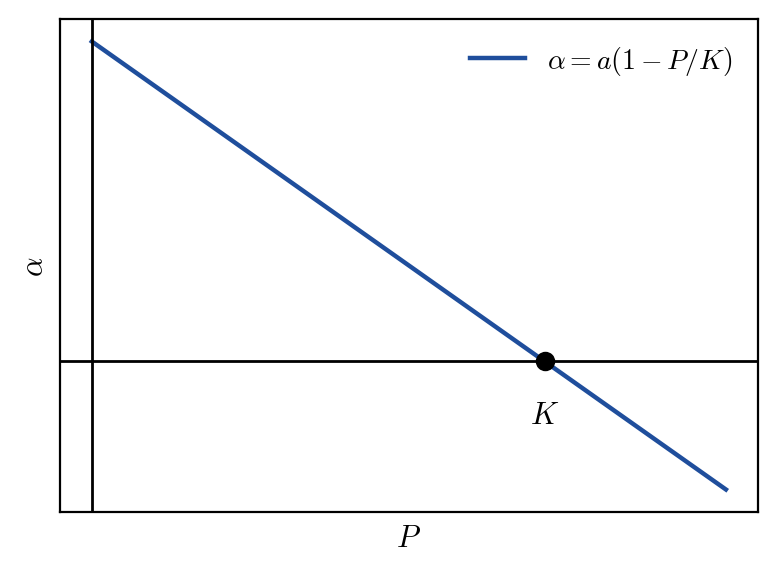
\includegraphics[width=0.4\textwidth]{tasa-logistica.png}
  \caption{Tasa logística $\alpha(P) = a\left(1 - \frac{P}{K}\right)$ como función de la población $P$.}
  \label{fig:tasa-logistica}
\end{figure}
Esta elección conduce a la ecuación logística
$$
\dot P = a\left(1 - \frac{P}{K}\right) P,
$$
cuyo comportamiento contrasta fuertemente con el del modelo malthusiano, como se ilustra en la Figura~\ref{fig:maltus-logistico}.
\begin{figure}[ht]
  \centering
  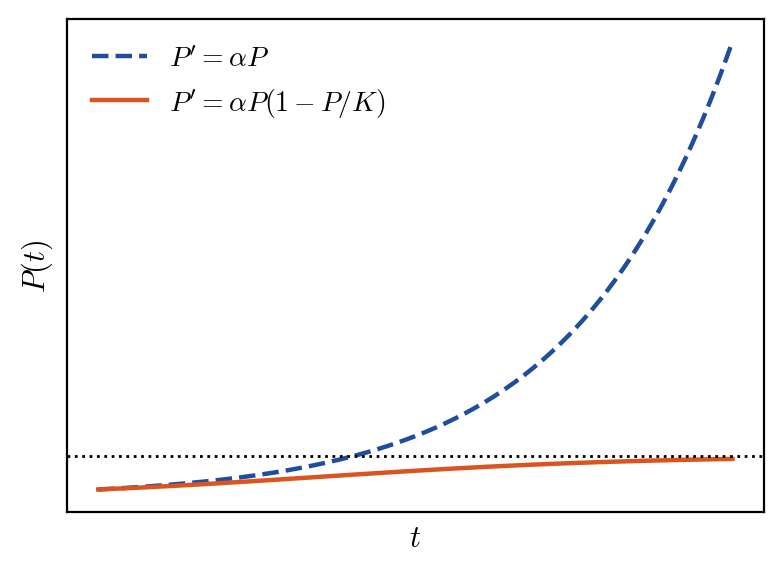
\includegraphics[width=0.4\textwidth]{maltus-vs-logistico.png}
  \caption{Comparación entre el modelo malthusiano y el modelo logístico.}
  \label{fig:maltus-logistico}
\end{figure}


Un paso fundamental en el análisis de modelos matemáticos es el proceso de \emph{adimensionalización}. Aun cuando el modelo logístico es lo suficientemente simple como para analizarse directamente en términos de los parámetros $a$ y $K$, resulta conveniente reducir el número de parámetros del sistema con el fin de simplificar su estudio y resaltar los mecanismos esenciales de la dinámica.

En este caso, en lugar de trabajar con la función $P(t)$, que representa el número absoluto de individuos, introducimos la variable adimensional
$$
p(t) = \frac{P(t)}{K},
$$
que mide la proporción de individuos con respecto a la capacidad de carga de la región.

Expresado en términos de la variable $p$, el modelo logístico adopta la forma
$$
\dot p = a(1 - p)p,
$$
en la cual ha desaparecido explícitamente el parámetro $K$. Si además medimos el tiempo en unidades de $1/a$ (es decir, $\tau = at$), desaparece también $a$: el modelo logístico no tiene, en realidad, ningún parámetro esencial. Todos los modelos logísticos son el mismo, salvo un cambio de escala en la población y en el tiempo.

\subsection*{La recta de fase}

La ecuación logística se puede resolver explícitamente (ver los ejercicios de laboratorio), pero lo que nos interesa ahora es un método que funcione aunque no sepamos resolver. Para una ecuación escalar $\dot p = f(p)$ alcanza con mirar el signo de $f$. Los ceros de $f$ son los \emph{equilibrios}: si $p(0)=p^*$ con $f(p^*)=0$, la solución es constante. Entre dos ceros consecutivos $f$ tiene signo constante, de modo que la solución es monótona: crece si $f>0$ y decrece si $f<0$. Como las soluciones no pueden cruzarse (por la unicidad de soluciones, que se repasa en el Capítulo \ref{cap:flujo}), una solución que empieza entre dos equilibrios queda atrapada entre ellos para siempre y converge, monótonamente, al equilibrio hacia el que apunta el signo de $f$.

Toda esta información se resume en la \emph{recta de fase}: se dibuja la recta real, se marcan los equilibrios y, en cada intervalo, una flecha en la dirección en que se mueve $p$. Para la logística, $f(p) = a(1-p)p$ se anula en $p=0$ y $p=1$; es negativa para $p<0$ (sin sentido biológico), positiva en $(0,1)$ y negativa para $p>1$. Luego, toda solución con $0<p(0)<1$ crece hacia $1$, y toda solución con $p(0)>1$ decrece hacia $1$: el equilibrio $p=1$ (la capacidad de carga) atrae a todas las soluciones con dato inicial positivo, y el equilibrio $p=0$ las repele. Esto es exactamente lo que se observa en la Figura~\ref{fig:logistico-condiciones-iniciales}.

\figpendiente{Recta de fase de la ecuación logística}{Recta real con los equilibrios $p=0$ y $p=1$ marcados y flechas indicando el sentido del movimiento en cada intervalo; debajo, el gráfico de $f(p)=a(1-p)p$.}

\begin{figure}[ht]
  \centering
  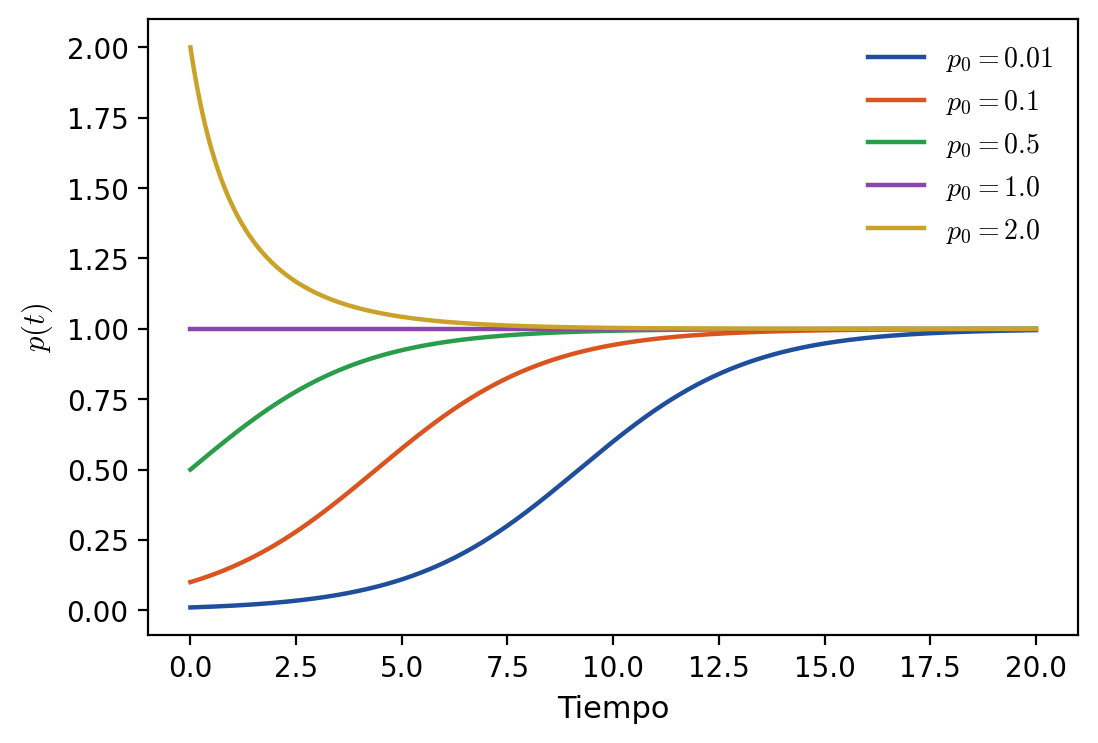
\includegraphics[width=0.6\textwidth]{logistica.png}
  \caption{Solución de la ecuación logística para diferentes condiciones iniciales.}
  \label{fig:logistico-condiciones-iniciales}
\end{figure}

La recta de fase resuelve por completo cualquier ecuación escalar autónoma: el comportamiento a largo plazo de toda solución es converger a un equilibrio, o escapar a infinito. En particular, en dimensión uno \emph{no puede haber oscilaciones}. Para verlas hay que pasar a sistemas de dos ecuaciones, que es lo que hacemos a continuación.

\section{Lotka--Volterra: primer modelo}\label{sec:LV1}

Consideramos ahora un sistema formado por dos poblaciones, que denotamos por $H$ y $P$. La variable $H(t)$ representa una población de herbívoros, mientras que $P(t)$ describe una población de predadores. Denotamos por $\alpha_H$ y $\alpha_P$ las tasas de crecimiento de las poblaciones de herbívoros y predadores, respectivamente.

Las hipótesis básicas del modelo son las siguientes:
\begin{itemize}
\item En ausencia de predadores, la población de herbívoros crece a tasa constante; sin embargo, su tasa de crecimiento disminuye monótonamente a medida que aumenta la población de predadores.

\item En ausencia de herbívoros, la población de predadores decae a tasa constante; en cambio, su tasa de crecimiento aumenta monótonamente con el tamaño de la población de herbívoros.
\end{itemize}

La elección más simple que refleja estas hipótesis conduce a las expresiones
$$
\alpha_H = b - sP, \qquad \alpha_P = -d + es\,H.
$$

Los parámetros del modelo admiten la siguiente interpretación:
\begin{itemize}
\item $b$ es la tasa latente de nacimientos de los herbívoros (\emph{birth rate});

\item $d$ es la tasa latente de mortalidad de los predadores (\emph{death rate});

\item $s$ mide la eficiencia con la cual los predadores encuentran presas (\emph{searching efficiency});

\item $e$ es la eficiencia con la cual el consumo de presas se traduce en nuevos predadores.
\end{itemize}

Bajo estas hipótesis, el modelo de Lotka--Volterra adopta la forma
$$
\begin{cases}
\dot H = bH - sPH,\\[4pt]
\dot P = -dP + es\,PH.
\end{cases}
$$

Este sistema depende de cuatro parámetros, por lo que resulta conveniente adimensionalizarlo con el fin de reducir el número de grados de libertad y facilitar su análisis cualitativo.


En particular, introducimos las variables adimensionales
$$
h = \frac{Hes}{d}, \qquad p = \frac{Ps}{b}, \qquad \tau = \sqrt{bd}\, t,
$$
y el parámetro
$$
\rho = \sqrt{\frac{b}{d}}.
$$
En términos de estas variables, el sistema se escribe como
\begin{equation}\label{LV1}
\begin{cases}
h' = \rho\, h(1 - p),\\[4pt]
p' = -\dfrac{1}{\rho}\, p(1 - h),
\end{cases}
\end{equation}
donde $h' = \mathrm{d}h/\mathrm{d}\tau$ y $p' = \mathrm{d}p/\mathrm{d}\tau$. La verificación de este cambio de variables queda como ejercicio.


Observamos que, en su forma adimensional, el sistema depende de un único parámetro $\rho$, lo que simplifica notablemente el estudio de su dinámica.

\subsection{Análisis del modelo: equilibrios y nulclinas}\label{sec:LV1-analisis}

El análogo de la recta de fase para un sistema en el plano es el \emph{diagrama de fases}: en cada punto $(h,p)$ del plano el sistema \eqref{LV1} define un vector $(h',p')$, y las soluciones son curvas tangentes a ese campo de vectores. Empecemos por los puntos donde el campo se anula, los \emph{equilibrios}. Resolviendo $h'=p'=0$ obtenemos dos:
$$
(h,p)=(0,0)\qquad \text{y}\qquad (h,p)=(1,1).
$$
El primero es la extinción de ambas especies; el segundo, la coexistencia.

Para orientarnos en el resto del plano usamos las \emph{nulclinas}: las curvas donde una de las dos derivadas se anula. La nulclina de $h$ (donde $h'=0$) está formada por la recta $h=0$ y la recta $p=1$; la de $p$ (donde $p'=0$) por la recta $p=0$ y la recta $h=1$. Los equilibrios son las intersecciones de una nulclina de $h$ con una de $p$. Las nulclinas dividen el cuadrante $h,p>0$ en cuatro regiones, y en cada una de ellas el signo de $(h',p')$ es constante:
\begin{itemize}
\item si $h>1$ y $p<1$ (muchas presas, pocos predadores): $h'>0$ y $p'>0$, ambas poblaciones crecen;
\item si $h>1$ y $p>1$: $h'<0$ y $p'>0$, los predadores siguen creciendo pero las presas empiezan a bajar;
\item si $h<1$ y $p>1$: $h'<0$ y $p'<0$, ambas decrecen;
\item si $h<1$ y $p<1$: $h'>0$ y $p'<0$, las presas se recuperan y los predadores siguen bajando.
\end{itemize}
Recorriendo las cuatro regiones en este orden, las trayectorias giran en sentido antihorario alrededor del punto $(1,1)$. Observemos también que los ejes son invariantes: si $p=0$ entonces $p'=0$ y $h$ crece exponencialmente (no hay predadores); si $h=0$, entonces $h'=0$ y $p$ decae exponencialmente. En particular, el origen atrae a las trayectorias que vienen por el eje $p$ y repele a las que salen por el eje $h$.

\subsection{Una cantidad conservada}

El análisis de signos dice que las trayectorias giran alrededor de $(1,1)$, pero no si se acercan a él, se alejan o vuelven sobre sí mismas. Para decidirlo buscamos una cantidad que no cambie a lo largo de las soluciones. Dividiendo las dos ecuaciones de \eqref{LV1},
$$
\frac{dp}{dh} = -\frac{1}{\rho^2}\,\frac{p(1-h)}{h(1-p)},
$$
que es una ecuación de variables separables:
$$
\frac{1-p}{p}\,dp = -\frac{1}{\rho^2}\,\frac{1-h}{h}\,dh
\qquad\Longrightarrow\qquad
\ln p - p = -\frac{1}{\rho^2}(\ln h - h) + \text{cte}.
$$
Es decir, la función
\begin{equation}\label{eq:LV1-integral}
\Hc(h,p) = (h - \ln h) + \rho^2\,(p - \ln p)
\end{equation}
es constante a lo largo de cada trayectoria (se verifica directamente derivando $\Hc(h(\tau),p(\tau))$ y usando \eqref{LV1}; queda como ejercicio). La función $\Hc$ tiene un único mínimo en $(1,1)$ y tiende a $+\infty$ cuando $h$ o $p$ tienden a $0$ o a $+\infty$, así que sus curvas de nivel son curvas cerradas alrededor de $(1,1)$. Cada trayectoria está contenida en una de esas curvas y, como recorre la curva girando siempre en el mismo sentido, la recorre entera: \emph{todas las soluciones con $h(0),p(0)>0$ son periódicas}. Esto es lo que muestra la Figura~\ref{fig:LV1}.

\begin{figure}[ht]
  \centering
  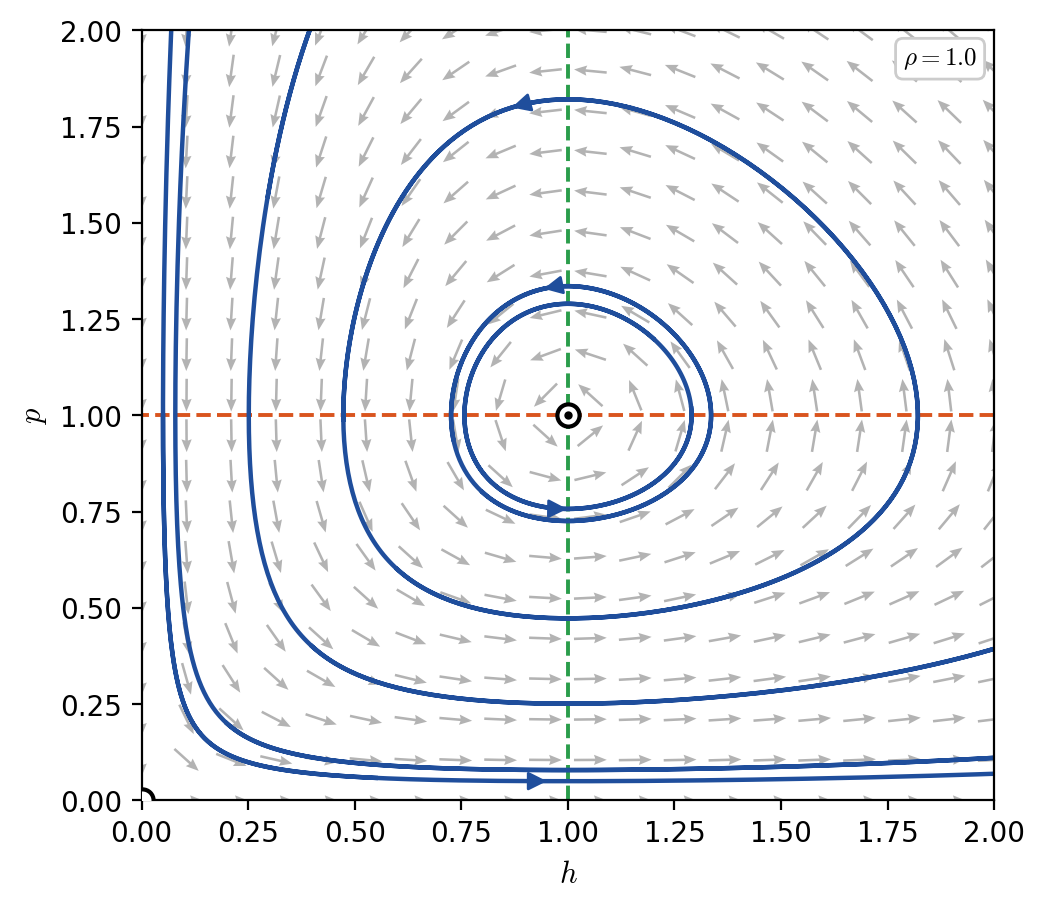
\includegraphics[width=0.6\textwidth]{LV1.png}
  \caption{Diagrama de fases para el modelo \eqref{LV1}. Los ejes corresponden a $h$ (horizontal) y $p$ (vertical). Las trayectorias son las curvas de nivel de $\Hc$.}
  \label{fig:LV1}
\end{figure}

Vale la pena detenerse en lo que acabamos de obtener: sin resolver el sistema, sabemos que las dos poblaciones oscilan indefinidamente, con una amplitud que depende sólo de la condición inicial, y que el equilibrio $(1,1)$ es \emph{estable} en el sentido de que las trayectorias que empiezan cerca de él se mantienen cerca (están sobre curvas de nivel pequeñas), aunque nunca convergen a él. Este tipo de equilibrio, rodeado de órbitas cerradas, se llama \emph{centro}. Notemos que esta situación es muy delicada: como vamos a ver enseguida, la más pequeña modificación del modelo destruye las órbitas cerradas.

\section{Lotka--Volterra con crecimiento logístico}\label{sec:LV2}

El modelo clásico de Lotka--Volterra asume que, en ausencia de predadores, la población de herbívoros crece a tasa constante, es decir, sigue un modelo malthusiano. Como ya vimos, esta hipótesis resulta poco realista para describir la evolución de poblaciones en intervalos de tiempo largos.

Una corrección natural consiste en reemplazar el crecimiento malthusiano de los herbívoros por un crecimiento logístico, incorporando una capacidad de carga del medio. El modelo resultante queda entonces
\begin{equation}\label{eq:LV-logistico}
\begin{cases}
\dot H = bH\left(1-\frac{H}{K}\right) - sPH,\\
\dot P = -dP + es PH,
\end{cases}
\end{equation}
donde $K$ denota la capacidad de carga del ambiente.


Utilizando las mismas variables adimensionales introducidas en la sección anterior y definiendo
$$
k = \frac{Kes}{d},
$$
que representa la capacidad de carga adimensional, el sistema puede reescribirse como
\begin{equation}\label{LV2}
\begin{cases}
\displaystyle h' = \rho h\left(1-\frac{h}{k}-p\right),\\[6pt]
p' = -\frac{1}{\rho}p(1-h).
\end{cases}
\end{equation}

Observemos que, para valores $k\gg 1$, este sistema constituye una pequeña perturbación del modelo de Lotka--Volterra clásico \eqref{LV1}.

\subsection*{Equilibrios y nulclinas}

Las nulclinas de $h$ son ahora la recta $h=0$ y la recta $p = 1 - h/k$; las de $p$ siguen siendo $p=0$ y $h=1$. Sus intersecciones dan los puntos de equilibrio del sistema \eqref{LV2}:
$$
\begin{bmatrix}
0\\
0
\end{bmatrix}, \qquad
\begin{bmatrix}
k\\
0
\end{bmatrix}, \qquad
\begin{bmatrix}
1\\
1-\frac{1}{k}
\end{bmatrix}.
$$
El segundo es nuevo respecto de \eqref{LV1}: sin predadores, los herbívoros ya no crecen indefinidamente sino que se estabilizan en la capacidad de carga. Notemos que el equilibrio de coexistencia $\left(1,1-\frac{1}{k}\right)^t$ sólo tiene sentido biológico cuando $k>1$: si la capacidad de carga es menor que $1$, la nulclina $p=1-h/k$ corta al eje $h$ antes de llegar a $h=1$ y no hay equilibrio con ambas poblaciones positivas. Además, cuando $k\to\infty$, el sistema \eqref{LV2} y sus equilibrios convergen formalmente a los del modelo \eqref{LV1}.

El análisis de signos es análogo al de la sección anterior, con una diferencia importante: la nulclina $p=1-h/k$ está inclinada, y eso rompe la simetría que en \eqref{LV1} hacía cerrar las órbitas. De hecho, la cantidad \eqref{eq:LV1-integral} ya no se conserva: a lo largo de las soluciones de \eqref{LV2} se tiene $\dot{\Hc} = -\frac{\rho}{k}h(h-1)$ (ejercicio), que cambia de signo según $h$ sea mayor o menor que $1$, así que $\Hc$ no es ni constante ni monótona. ¿Qué hacen entonces las trayectorias? Las simulaciones responden con claridad y distinguen tres casos.

\noindent{\underline{Caso $0<k<1$:}} Sólo hay dos equilibrios en el cuadrante, $(0,0)$ y $(k,0)$. Las simulaciones (Figura~\ref{fig:LVk<1}) muestran que todas las trayectorias con $h(0),p(0)>0$ convergen a $(k,0)$: los predadores se extinguen y los herbívoros tienden a la capacidad de carga. Se puede ver por qué con el análisis de signos: si $k<1$ entonces $1-h<0$ obliga a $h>1>k$, y en esa región $h'<0$; una vez que $h<1$, se tiene $p'<0$ para siempre, así que $p$ decrece monótonamente, y $h$ termina comportándose como una logística.
\begin{figure}[ht]
  \centering
  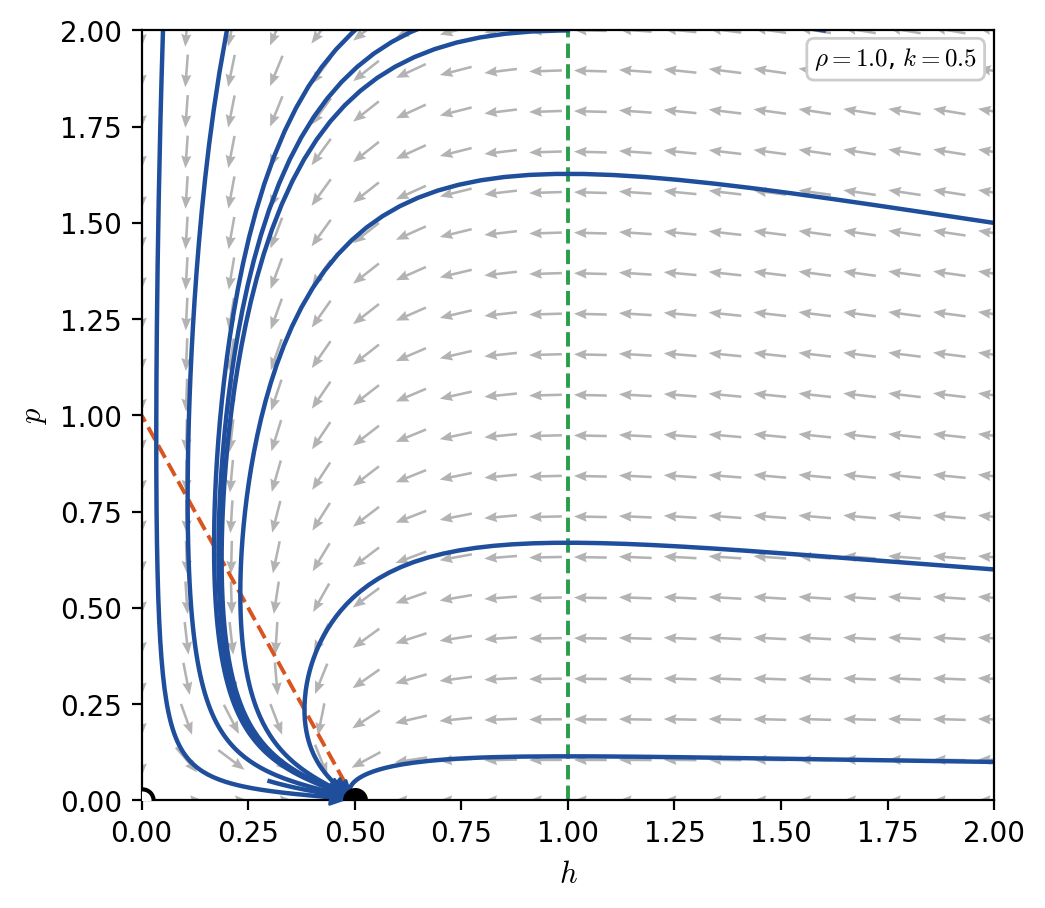
\includegraphics[width=0.6\textwidth]{LVk<1.png}
  \caption{Diagrama de fases para el modelo \eqref{LV2} para $k<1$ (en la figura, $k=0.5$).}
  \label{fig:LVk<1}
\end{figure}
Observemos que con esta elección de parámetros (que representa una baja capacidad de carga, independientemente del parámetro $\rho$) el modelo predice que la población de predadores se extingue y la población de herbívoros converge al equilibrio del modelo logístico $h=k$.

\noindent{\underline{Caso $k=1$:}}
Los equilibrios $(k,0)$ y $(1,1-1/k)$ coinciden en $(1,0)$. Las simulaciones (Figura~\ref{fig:LVk=1}) muestran el mismo comportamiento que en el caso anterior, pero la convergencia es mucho más lenta: las trayectorias se acercan a $(1,0)$ ``rozando'' el eje. Es un caso límite, y lo volveremos a encontrar cuando estudiemos bifurcaciones.
\begin{figure}[ht]
  \centering
  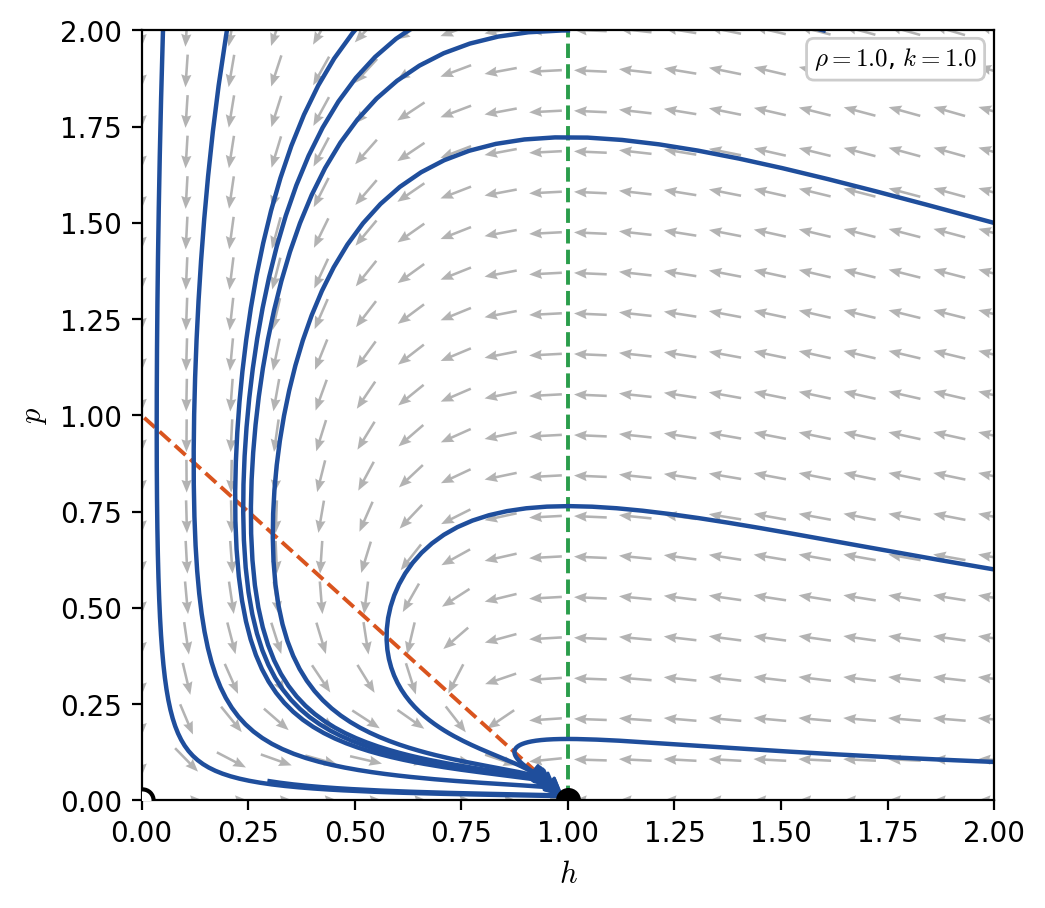
\includegraphics[width=0.6\textwidth]{LVk=1.png}
  \caption{Diagrama de fases para el modelo \eqref{LV2} para $k=1$.}
  \label{fig:LVk=1}
\end{figure}

\noindent{\underline{Caso $k>1$:}}
Aparece el equilibrio de coexistencia y las simulaciones muestran que atrae a todas las trayectorias con ambas poblaciones positivas. Pero la forma en que se acercan depende de los parámetros: para algunos valores de $\rho$ y $k$ las trayectorias se acercan sin dar vueltas (Figura~\ref{fig:LVk>1-1}), y para otros lo hacen en espiral, oscilando alrededor del equilibrio con oscilaciones cada vez más chicas (Figura~\ref{fig:LVk>1-2}). Con las herramientas de este capítulo no podemos determinar cuál de las dos situaciones ocurre para un par $(\rho,k)$ dado; cuando desarrollemos más la teoría vamos a poder calcular exactamente la curva que separa un comportamiento del otro.
\begin{figure}[ht]
  \centering
  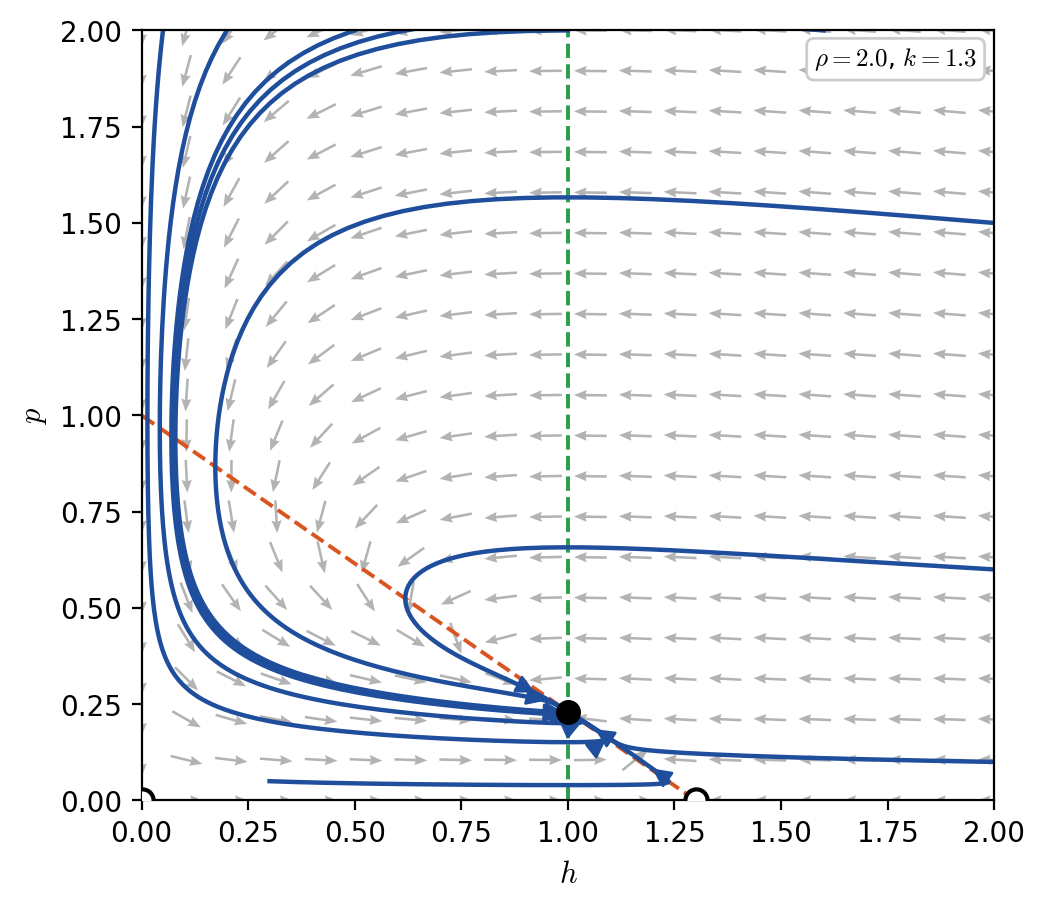
\includegraphics[width=0.6\textwidth]{LVk>1-1.png}
  \caption{Diagrama de fases para el modelo \eqref{LV2} para $k>1$: acercamiento monótono al equilibrio de coexistencia (en la figura, $k=1.3$).}
  \label{fig:LVk>1-1}
\end{figure}
\begin{figure}[ht]
  \centering
  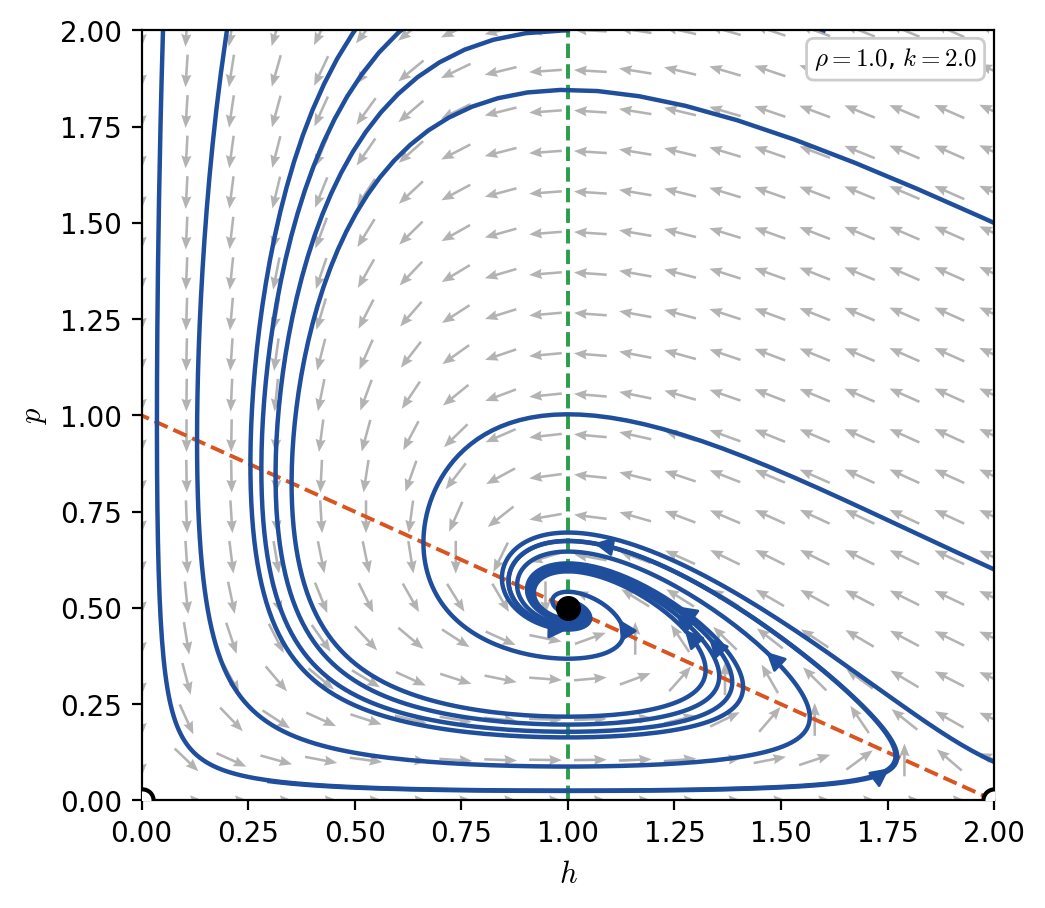
\includegraphics[width=0.6\textwidth]{LVk>1-2.png}
  \caption{Diagrama de fases para el modelo \eqref{LV2} para $k>1$: acercamiento oscilatorio al equilibrio de coexistencia (en la figura, $k=2$).}
  \label{fig:LVk>1-2}
\end{figure}

Lo que sí podemos afirmar es que la introducción de la capacidad de carga cambió cualitativamente el modelo: las oscilaciones sostenidas de \eqref{LV1} desaparecen y son reemplazadas por un equilibrio al que todo converge. Para un científico de datos esto tiene una consecuencia práctica: si en los datos se observan oscilaciones que no se amortiguan, el modelo \eqref{LV2} no las va a reproducir, por más que se ajusten sus parámetros.

\section{Ciclos límite}\label{sec:ciclo_limite}

En los modelos discutidos hasta ahora, la dinámica a largo plazo estaba dominada por equilibrios: las poblaciones tendían a estados estacionarios o se extinguían (con la excepción de \eqref{LV1}, cuyas oscilaciones son un caso frágil, como acabamos de ver). Sin embargo, en muchos sistemas reales —biológicos, químicos o sociales— se observan oscilaciones persistentes que no se amortiguan con el tiempo, y cuya amplitud no depende de cómo empezó el sistema. Este tipo de comportamiento no puede describirse únicamente mediante puntos de equilibrio.

Para ilustrar este fenómeno, consideramos una variante del sistema de Lotka--Volterra propuesta recientemente para modelar con mayor fidelidad ciertos experimentos con poblaciones bacterianas:
\begin{equation}\label{bacteria}
\begin{cases}
\dot H = r_H H\left(1-\frac{H}{K}\right) - \dfrac{a_H PH}{b+H},\\[6pt]
\dot P = \dfrac{a_P PH}{b+H} - cP.
\end{cases}
\end{equation}

El término racional $\frac{PH}{b+H}$ modela un efecto de saturación en la interacción entre ambas poblaciones: cuando hay muchas presas, cada predador no puede comer más allá de cierto límite. Observemos que, cuando $H\ll b$, este modelo puede interpretarse como una perturbación del modelo de Lotka--Volterra con crecimiento logístico \eqref{eq:LV-logistico}.

El sistema \eqref{bacteria} posee dos equilibrios triviales, $(0,0)$ y $(K,0)$. Además, admite un único equilibrio no trivial, que denotamos por $(H^*,P^*)$ (verifique esta afirmación).

Introducimos las variables adimensionales
$$
h = \frac{H}{H^*},\qquad p = \frac{P}{P^*},\qquad \tau = r_H t,
$$
y redefinimos los parámetros como
$$
k = \frac{K}{H^*},\quad \beta = \frac{b}{H^*},\quad \gamma = \frac{c}{r_H},\quad
\alpha_h = \left(1-\frac{1}{k}\right)(\beta+1),\quad
\alpha_p = \gamma(\beta+1).
$$

En estas variables, el sistema queda
\begin{equation}\label{bacteria2}
\begin{cases}
h' = h\left(1-\frac{h}{k}\right) - \dfrac{\alpha_h ph}{\beta + h},\\[6pt]
p' = \dfrac{\alpha_p ph}{\beta + h} - \gamma p.
\end{cases}
\end{equation}
Este sistema tiene un único equilibrio no trivial en $(1,1)$.

Las nulclinas de \eqref{bacteria2} son, para $h$, la recta $h=0$ y la curva $p = \frac{(\beta+h)(1-h/k)}{\alpha_h}$ (una parábola invertida que corta al eje en $h=k$), y para $p$, la recta $p=0$ y la recta vertical $h=\beta\gamma/(\alpha_p-\gamma) = 1$. La novedad respecto de \eqref{LV2} es que la nulclina de $h$ ya no es una recta sino una parábola con vértice en $h = (k-\beta)/2$. El equilibrio $(1,1)$ puede caer sobre la rama descendente de la parábola, a la derecha del vértice (si $k<2+\beta$), o sobre la rama ascendente, a la izquierda del vértice (si $k>2+\beta$), y esa posición resulta decisiva.

Las simulaciones muestran lo siguiente. Cuando $k$ es moderado, las trayectorias convergen en espiral al equilibrio $(1,1)$ (Figura~\ref{fig:bacteria1}). Cuando $k$ supera un cierto valor crítico $k_c$, el equilibrio deja de atraer: las trayectorias que empiezan cerca de él se alejan en espiral, y las que empiezan lejos se acercan, y unas y otras convergen a la misma órbita cerrada (Figura~\ref{fig:bacteria2}). Esa órbita cerrada aislada, a la que convergen las trayectorias vecinas, se llama \emph{ciclo límite}. A diferencia de las órbitas de \eqref{LV1}, su amplitud y su período no dependen de la condición inicial: son propiedades del sistema.
\begin{figure}[ht]
\centering
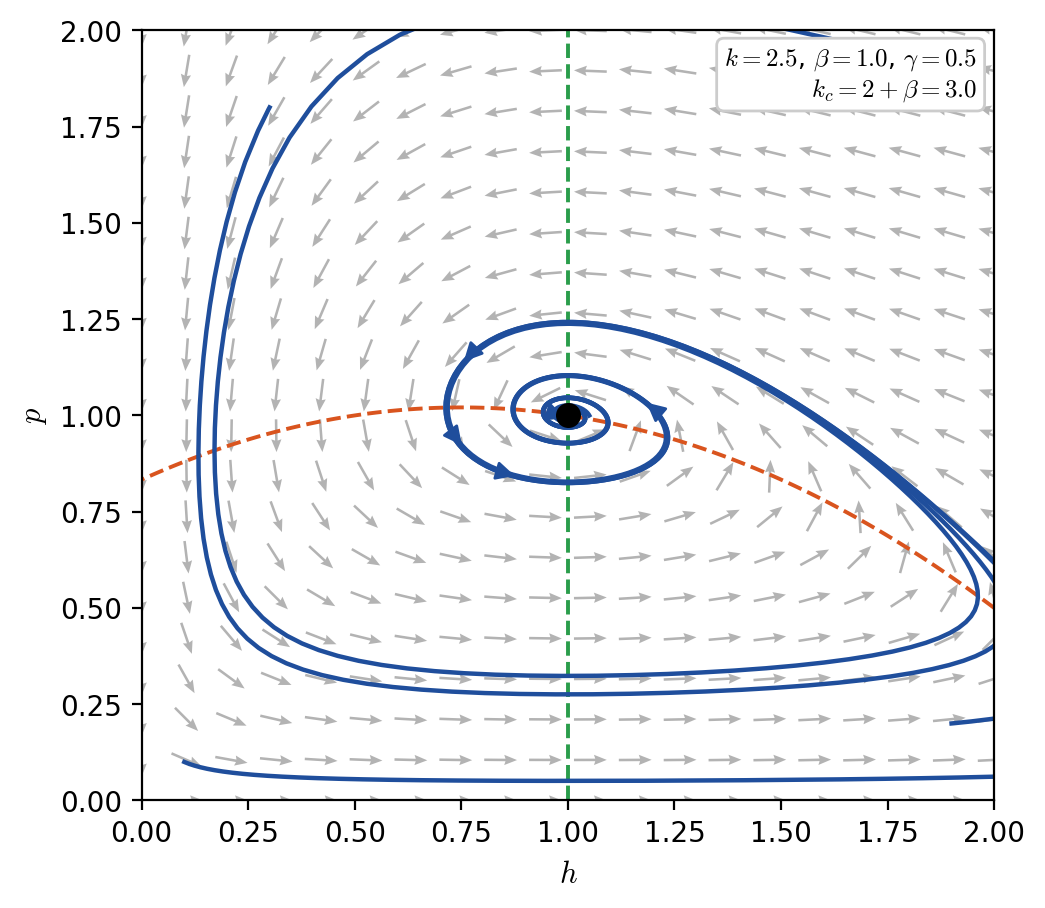
\includegraphics[width=0.6\textwidth]{bacteria1.png}
\caption{Diagrama de fases para el modelo \eqref{bacteria2} cuando $k<k_c$: las trayectorias convergen al equilibrio $(1,1)$.} \label{fig:bacteria1}
\end{figure}
\begin{figure}[ht]
  \centering
  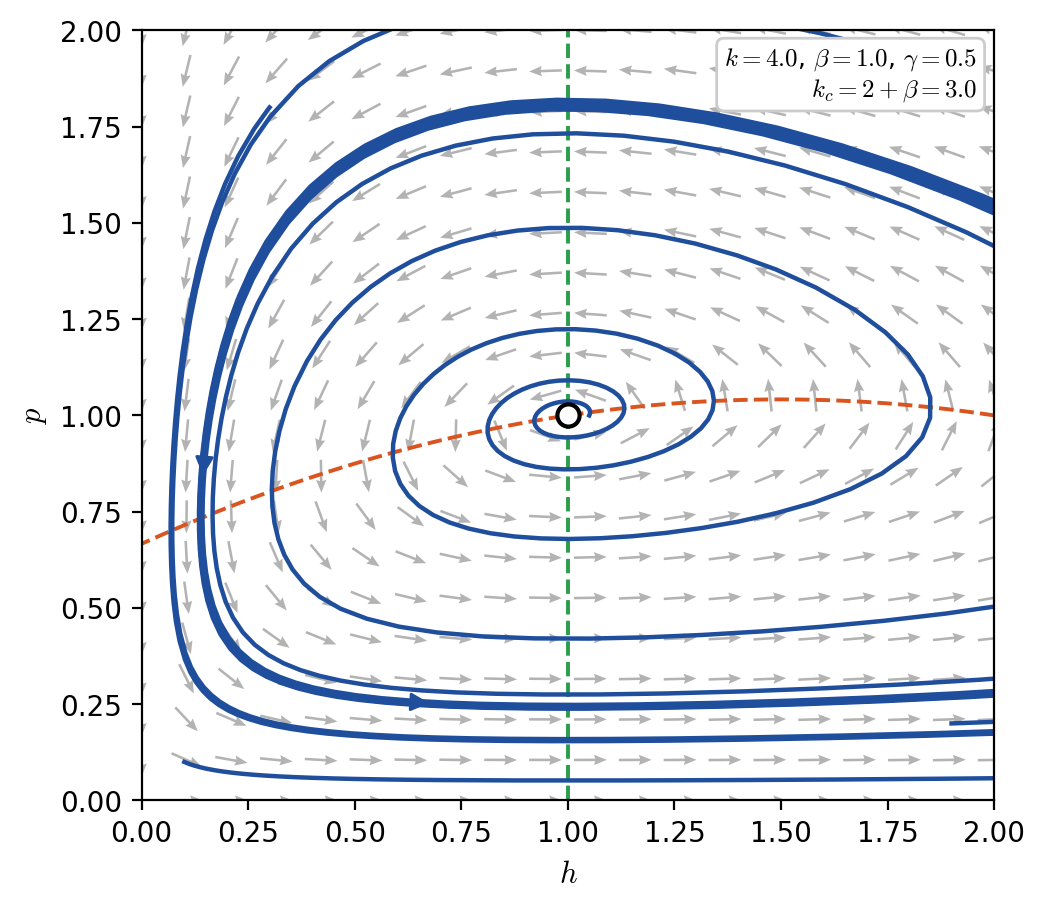
\includegraphics[width=0.6\textwidth]{bacteria2.png}
  \caption{Aparición de un ciclo límite en el sistema \eqref{bacteria2} cuando $k>k_c$.}
  \label{fig:bacteria2}
\end{figure}

Las simulaciones sugieren que el valor crítico es $k_c = 2+\beta$, es decir, el valor para el cual el equilibrio pasa por el vértice de la parábola. Con las herramientas de este capítulo no podemos demostrarlo ni explicar por qué la pérdida de estabilidad del equilibrio viene acompañada del nacimiento de un ciclo. Cuando desarrollemos más la teoría vamos a poder hacer ambas cosas; este ejemplo va a ser nuestro modelo de referencia para el fenómeno.

\section{El modelo SIR}\label{sec:SIR}

Volvemos ahora al primer problema conductor, presentado en la Sección \ref{sec:conductor-SIR}. Trabajamos con las fracciones $s,i,r$ de susceptibles, infectados y removidos, que satisfacen
\begin{equation}\label{SIR}
\begin{cases}
\dot s = - \beta s i,\\
\dot i = \beta s i - \gamma i,\\
\dot r = \gamma i,
\end{cases}
\qquad s+i+r=1,
\end{equation}
con $\beta>0$ la tasa de contagio y $\gamma>0$ la tasa de remoción, y $R_0=\beta/\gamma$. Notemos que
\[
\frac{d}{dt}(s+i+r) = \dot s + \dot i + \dot r = 0,
\]
lo que confirma que la población total se conserva. La escala de tiempo natural del problema es $1/\gamma$, la duración media de la infección; midiendo el tiempo en esas unidades ($\tau=\gamma t$) el sistema queda con $R_0$ como único parámetro: $s' = -R_0 s i$, $i' = (R_0 s - 1) i$.

\subsection*{¿Hay epidemia?}

De la primera ecuación se deduce que $s(t)$ es una función decreciente. Por otra parte, de la ecuación para $i$ se observa que $i(t)$ es creciente si $s(t) > 1/R_0$ y decreciente si $s(t) < 1/R_0$. En particular, si el número inicial de susceptibles satisface $s_0 < 1/R_0$, como $s(t) \le s_0$ para todo $t$, la infección desaparece sin llegar a propagarse. En cambio, si $s_0 > 1/R_0$, el número de infectados crece inicialmente y luego decrece cuando $s(t)$ cae por debajo de $1/R_0$. En este caso se produce una epidemia.

\begin{obs}
Este fenómeno muestra que una epidemia ocurre sólo si la fracción inicial de individuos susceptibles supera el umbral $1/R_0$. Cuando la enfermedad es nueva, $s_0\simeq 1$, y la condición se lee simplemente: hay epidemia si y sólo si $R_0>1$, es decir, si cada infectado contagia en promedio a más de una persona. Una epidemia es menos probable cuando la tasa de remoción es alta en relación con la tasa de infección; esto ocurre, por ejemplo, cuando los individuos infectados son removidos rápidamente del proceso de contagio (aislamiento). La vacunación actúa sobre $s_0$: si se vacuna una fracción $v$ de la población, $s_0 = 1-v$, y la epidemia no se produce si $1-v<1/R_0$, es decir, si $v>1-1/R_0$. Esta es la fracción que hay que vacunar para lograr la llamada \emph{inmunidad de rebaño}.
\end{obs}

\begin{figure}[ht]
  \centering
  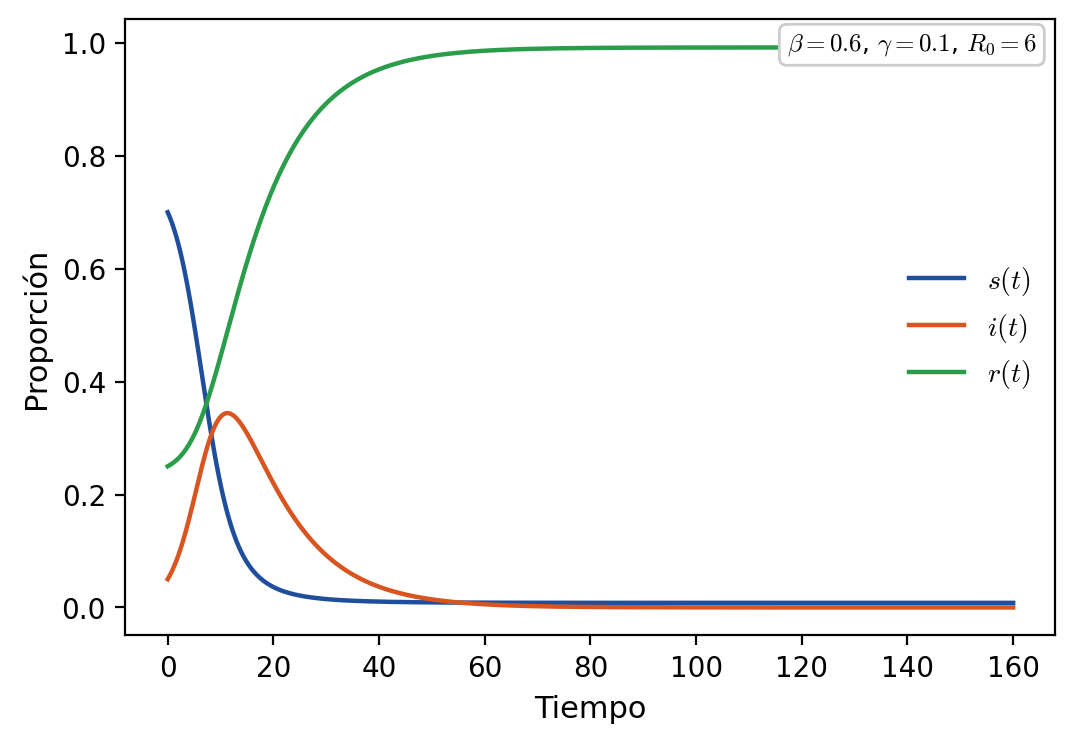
\includegraphics[width=0.6\textwidth]{SIR.png}
  \caption{Evolución temporal del modelo SIR con datos iniciales $s(0)=0.7$, $i(0)=0.05$, $r(0)=0.25$ y parámetros $\beta=0.6$ y $\gamma=0.1$ ($R_0=6$).}
  \label{fig:SIR}
\end{figure}

\subsection*{El plano de fases $(s,i)$ y el pico de la epidemia}

Como $r=1-s-i$, alcanza con seguir la trayectoria en el plano $(s,i)$. Dividiendo las dos primeras ecuaciones de \eqref{SIR},
$$
\frac{di}{ds} = -1 + \frac{1}{R_0 s},
$$
que se integra directamente: la cantidad
\begin{equation}\label{eq:SIR-conservada}
i + s - \frac{1}{R_0}\ln s
\end{equation}
es constante a lo largo de cada trayectoria. Las trayectorias son entonces las curvas de nivel de \eqref{eq:SIR-conservada} en el triángulo $s,i\ge 0$, $s+i\le 1$, recorridas con $s$ decreciente. Sobre cada una, $i$ alcanza su máximo cuando $s=1/R_0$ (Figura pendiente). Si la epidemia empieza con $s_0\simeq 1$ e $i_0\simeq 0$, la constante vale $1$, y el pico es
$$
i_{\max} = 1 - \frac{1}{R_0}\bigl(1+\ln R_0\bigr).
$$
Para $R_0=2$ el pico es del $15\%$ de la población; para $R_0=6$, del $53\%$.

\figpendiente{Plano de fases $(s,i)$ del modelo SIR}{Curvas de nivel de $i+s-\frac{1}{R_0}\ln s$ en el triángulo $s+i\le 1$, con la recta $s=1/R_0$ marcada y flechas indicando el sentido ($s$ decreciente). Dos o tres valores de $R_0$.}

\subsection*{¿Cuánta gente no se contagia?}

Analicemos ahora el comportamiento asintótico del sistema cuando $t \to \infty$.
\begin{itemize}
\item Como $s(t)>0$ y es decreciente, existe el límite $s(t)\to s_\infty\ge 0$.
\item La función $r(t)$ es creciente y está acotada superiormente por $1$, luego existe el límite $r(t)\to r_\infty$.
\item Como $s+i+r=1$, se deduce que $i(t)\to i_\infty = 1-s_\infty-r_\infty$. Y de hecho $i_\infty = 0$: si fuera positivo, $r$ crecería al menos linealmente, contradiciendo que está acotada. La epidemia siempre termina.
\end{itemize}

Finalmente, a partir de las ecuaciones para $s$ y $r$ obtenemos
\[
\frac{ds}{dr} = -R_0\, s,
\]
e integrando,
\[
s(t) = s_0 e^{-R_0 (r(t)-r(0))} \ge s_0 e^{-R_0} > 0.
\]
En particular, $s_\infty>0$: \emph{siempre queda una fracción de la población que no se infecta}. La epidemia no termina porque se agoten los susceptibles, sino porque quedan tan pocos que cada infectado ya no llega a contagiar a uno. Pasando al límite y usando $i_\infty=0$ (con $r(0)=0$), la fracción final de susceptibles es la solución de la ecuación
\begin{equation}\label{eq:SIR-final}
s_\infty = s_0\, e^{-R_0(1-s_\infty)},
\end{equation}
llamada \emph{relación del tamaño final}. Es una ecuación trascendente que se resuelve numéricamente; para $s_0\simeq 1$ y $R_0=2$ da $s_\infty\simeq 0.20$ (se contagia el $80\%$), y para $R_0=1.5$, $s_\infty\simeq 0.42$.

\begin{volvemos}{la epidemia}
Con las herramientas de este capítulo respondimos las tres primeras preguntas de la Sección \ref{sec:conductor-SIR}: hay epidemia si y sólo si $R_0 s_0>1$; el pico ocurre cuando los susceptibles bajan a $1/R_0$ y su altura está dada por $i_{\max}$; y la fracción que no se contagia es la solución de \eqref{eq:SIR-final}. Las tres respuestas dependen de un único número, $R_0$, que es por lo tanto el parámetro que hay que estimar a partir de los datos. Lo que todavía no sabemos decir es qué pasa con los equilibrios del sistema: todo punto $(s,0)$ es un equilibrio de \eqref{SIR}, y las trayectorias convergen a alguno de ellos, pero no tenemos un lenguaje para describir su estabilidad. Ese lenguaje es el que desarrollamos en los capítulos que siguen.
\end{volvemos}

\section{Comentarios finales}

En este capítulo analizamos una serie de modelos clásicos provenientes de la biología y la epidemiología, cuyo denominador común es que describen la evolución temporal de poblaciones mediante sistemas de ecuaciones diferenciales ordinarias no lineales. A pesar de la simplicidad de sus hipótesis, estos modelos exhiben una gran variedad de comportamientos dinámicos que no aparecen en modelos lineales.

El modelo logístico muestra cómo la introducción de una capacidad de carga conduce naturalmente a la existencia de equilibrios estables y a la saturación del crecimiento poblacional. Los modelos de Lotka--Volterra, en sus distintas variantes, ilustran la interacción entre especies y ponen de manifiesto la aparición de oscilaciones, cambios de estabilidad y, en algunos casos, ciclos límite. El modelo SIR, por su parte, introduce la noción de umbral y muestra cómo pequeñas variaciones en los parámetros o en las condiciones iniciales pueden determinar si una epidemia se propaga o se extingue.

Vale la pena hacer un balance de lo que pudimos y no pudimos hacer. Con el signo de las derivadas, las nulclinas y las cantidades conservadas resolvimos por completo la ecuación logística, el modelo de Lotka--Volterra clásico y el modelo SIR. Para el modelo con capacidad de carga y para el modelo de bacterias, en cambio, sólo pudimos describir lo que muestran las simulaciones: que las trayectorias convergen a un equilibrio, a veces oscilando y a veces no, o a un ciclo límite, según los parámetros. Para justificar esas observaciones y, sobre todo, para calcular los umbrales que separan un comportamiento de otro, hace falta una teoría que diga cómo se comporta un sistema \emph{cerca} de un equilibrio. Esa teoría es el objetivo de los próximos capítulos.

\chapter{Sistemas mecánicos}\label{sec:sistemas-mecanicos}

Una de las fuentes históricas y conceptuales más importantes de las ecuaciones diferenciales ordinarias (EDOs) es la mecánica clásica. En este capítulo introductorio mostramos cómo modelos mecánicos simples conducen, de manera natural, a ecuaciones diferenciales que describen la evolución temporal de un sistema.

El objetivo no es desarrollar una teoría completa de la mecánica newtoniana, sino ilustrar cómo las leyes físicas fundamentales se traducen en modelos matemáticos concretos. Estos ejemplos servirán como motivación y referencia a lo largo del curso, tanto para el análisis teórico como para la interpretación cualitativa de las soluciones.

\section{Leyes de Newton}

El punto de partida es la segunda ley de Newton, que afirma que la fuerza total que actúa sobre una partícula es igual a la masa de la partícula multiplicada por su aceleración:
\[
F = m \ab.
\]

Si denotamos por $\xx(t)$ la posición de la partícula en función del tiempo, la aceleración es la segunda derivada de la posición, $\ab = \ddot \xx(t)$. Por lo tanto, la segunda ley de Newton puede escribirse como
\[
m \ddot\xx(t) = F(\xx(t), \dot\xx(t), t),
\]
donde hemos explicitado que la fuerza puede depender de la posición, de la velocidad y del tiempo. Esta ecuación es, en general, una ecuación diferencial ordinaria de segundo orden.

\section{El oscilador armónico}

Uno de los ejemplos más simples y fundamentales es el oscilador armónico. Consideremos una partícula unida a un resorte ideal, de constante elástica $k > 0$, que se mueve sin fricción. La ley de Hooke establece que la fuerza ejercida por el resorte es proporcional al desplazamiento respecto de la posición de equilibrio y apunta en sentido contrario (ver Figura~\ref{fig:resorte}):
\[
F = -k x.
\]

\begin{figure}[ht]
  \centering
  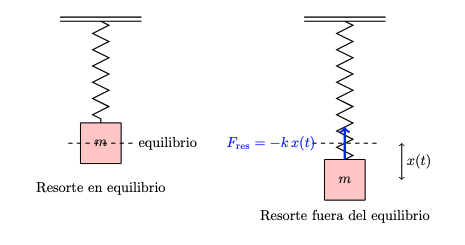
\includegraphics[width=0.6\textwidth]{Resorte.png}
  \caption{Modelo del oscilador armónico.}
  \label{fig:resorte}
\end{figure}

Aplicando la segunda ley de Newton, el desplazamiento $x(t)$ de la partícula respecto de la posición de equilibrio satisface la ecuación
\[
\ddot x(t) + k x(t) = 0.
\]
Esta es una EDO lineal de segundo orden con coeficientes constantes, cuyas soluciones describen un movimiento oscilatorio periódico. El oscilador armónico aparece en una enorme variedad de contextos físicos y matemáticos, y constituye un modelo de referencia para sistemas más complejos.

\section{El resorte con fricción}

En situaciones más realistas, el movimiento suele estar afectado por fuerzas disipativas. Un modelo simple de fricción es la fricción viscosa, en la cual la fuerza es proporcional y opuesta a la velocidad:
\[
F_{\text{fric}} = -\gamma \dot x(t), \qquad \gamma > 0.
\]

Si incorporamos esta fuerza al modelo del resorte, la ecuación de movimiento pasa a ser
\[
m \ddot x(t) + \gamma \dot x(t) + k x(t) = 0.
\]
Esta ecuación describe un oscilador armónico amortiguado. Dependiendo de los valores de los parámetros $m$, $\gamma$ y $k$, el sistema puede presentar distintos regímenes dinámicos, como oscilaciones amortiguadas o relajación monótona hacia el equilibrio.

\section{El péndulo simple}\label{sec:pendulo}

Otro ejemplo clásico es el péndulo simple. Consideremos una masa puntual suspendida de un hilo inextensible y sin masa, de longitud $\ell$, que oscila en un plano vertical bajo la acción de la gravedad. Si denotamos por $\theta(t)$ el ángulo que forma el hilo con la vertical, la ecuación de movimiento resulta
\[
\ddot \theta(t) + \frac{g}{\ell} \sin\theta(t) = 0,
\]
donde $g$ es la aceleración de la gravedad. Ver Figura~\ref{fig:pendulo}.

\begin{figure}[ht]
  \centering
  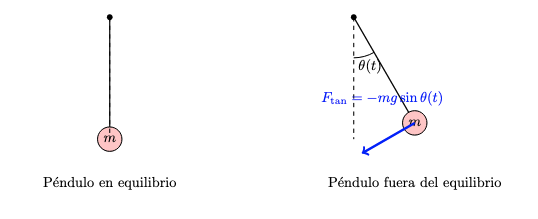
\includegraphics[width=0.6\textwidth]{Pendulo.png}
  \caption{Modelo del péndulo simple.}
  \label{fig:pendulo}
\end{figure}

A diferencia de los ejemplos anteriores, esta es una ecuación no lineal debido a la presencia del seno. Para oscilaciones pequeñas, es habitual aproximar $\sin\theta \approx \theta$, lo que conduce a la ecuación lineal
\[
\ddot \theta(t) + \frac{g}{\ell} \theta(t) = 0.
\]
Esta aproximación pone de manifiesto la estrecha relación entre el péndulo simple y el oscilador armónico.

\section{El péndulo amortiguado}\label{sec:pendulo_amortiguado}

Podemos combinar el modelo del péndulo con la presencia de fricción, por ejemplo debida a la resistencia del aire o a rozamientos en el punto de suspensión. Introduciendo un término disipativo proporcional a la velocidad angular, se obtiene la ecuación
\[
\ddot\theta(t) + \alpha \dot\theta(t) + \frac{g}{\ell} \sin\theta(t) = 0,
\]
con $\alpha > 0$.

Esta ecuación no lineal describe el péndulo amortiguado y da lugar a una dinámica rica, que incluye oscilaciones amortiguadas y convergencia al equilibrio.

\section{Circuitos eléctricos}\label{sec:circuitos}

Las mismas ecuaciones aparecen en un contexto completamente distinto: los circuitos eléctricos. Consideremos un circuito en serie con una resistencia $R$, una inductancia $L$ y un capacitor de capacidad $C$, alimentado por una fuente de voltaje $v(t)$. Si $x(t)$ es la corriente y $v_C(t)$ el voltaje en el capacitor, las relaciones constitutivas de cada componente son: la caída de voltaje en la resistencia es $Rx$ (ley de Ohm), en la inductancia es $L\dot x$, y la carga del capacitor verifica $C\dot v_C = x$. La ley de Kirchhoff (la suma de las caídas de voltaje a lo largo del circuito es igual al voltaje de la fuente) da
\[
L\dot x + Rx + v_C = v(t),\qquad C\dot v_C = x.
\]
Derivando la primera ecuación y usando la segunda se obtiene
\[
L\ddot x + R\dot x + \frac{1}{C}x = \dot v(t),
\]
que es exactamente la ecuación del oscilador armónico amortiguado y forzado, con la correspondencia $m\leftrightarrow L$, $\gamma\leftrightarrow R$, $k\leftrightarrow 1/C$. La inductancia juega el papel de la inercia, la resistencia el de la fricción y el capacitor el del resorte. En ausencia de fuente y de resistencia, la corriente oscila con frecuencia angular $1/\sqrt{LC}$, es decir, con período $2\pi\sqrt{LC}$.

En la Sección \ref{sec:conductor-vdP} vimos qué pasa cuando la resistencia se reemplaza por un elemento no lineal con característica $v_R(x) = -ax+bx^3$: se obtiene, luego de adimensionalizar, la ecuación de van der Pol
\begin{equation}\label{eq:vdP-cap3}
\ddot x + \lambda(x^2-1)\dot x + x = 0 .
\end{equation}
Comparándola con el oscilador amortiguado, el coeficiente de fricción es ahora $\lambda(x^2-1)$: negativo para $|x|<1$ y positivo para $|x|>1$. Volvemos sobre esto al final del capítulo.

\section{Reducción a un sistema de primer orden}

Las ecuaciones diferenciales ordinarias que surgen de modelos mecánicos suelen ser ecuaciones de segundo orden. Sin embargo, desde el punto de vista teórico y práctico, es conveniente reescribirlas como sistemas de ecuaciones diferenciales de primer orden. Esta reformulación permite un tratamiento unificado de los problemas de existencia y unicidad, y es la base del análisis cualitativo en el espacio de fases.

Consideremos una ecuación diferencial ordinaria escalar de segundo orden de la forma
\[
x''(t) = f\bigl(x(t), x'(t), t\bigr).
\]
Introduciendo la variable velocidad
\[
v(t) = x'(t),
\]
la ecuación anterior es equivalente al sistema
\[
\begin{cases}
x'(t) = v(t),\\
v'(t) = f\bigl(x(t), v(t), t\bigr).
\end{cases}
\]

De este modo, el estado del sistema en un instante dado queda determinado por el par $(x(t), v(t))$, y la evolución temporal puede interpretarse como una curva en el plano de fases.

Por ejemplo, el oscilador armónico
\[
m \ddot x(t) + k x(t) = 0
\]
puede escribirse como
\[
\begin{cases}
\dot x(t) = v(t),\\
\dot v(t) = -\dfrac{k}{m} x(t).
\end{cases}
\]

De manera análoga, el oscilador armónico amortiguado
\[
m \ddot x(t) + \gamma \dot x(t) + k x(t) = 0
\]
se transforma en
\[
\begin{cases}
\dot x(t) = v(t),\\
\dot v(t) = -\dfrac{k}{m} x(t) - \dfrac{\gamma}{m} v(t).
\end{cases}
\]

En el caso del péndulo simple,
\[
\ddot\theta(t) + \frac{g}{\ell}\sin\theta(t) = 0,
\]
la introducción de la velocidad angular $\omega(t) = \dot\theta(t)$ conduce al sistema no lineal
\[
\begin{cases}
\dot\theta(t) = \omega(t),\\
\dot\omega(t) = -\dfrac{g}{\ell}\sin\theta(t).
\end{cases}
\]

Y la ecuación de van der Pol \eqref{eq:vdP-cap3} se escribe como
\begin{equation}\label{eq:vdP-sistema}
\begin{cases}
\dot x = y,\\
\dot y = -x - \lambda(x^2-1)y .
\end{cases}
\end{equation}

Esta reformulación pone de manifiesto que tanto los sistemas lineales como los no lineales pueden tratarse dentro de un mismo marco conceptual. A lo largo del curso trabajaremos principalmente con sistemas de primer orden, ya que constituyen la forma estándar para el análisis cualitativo y los métodos numéricos.

\section{La energía como herramienta}\label{sec:energia-herramienta}

Para los sistemas mecánicos hay una cantidad que hace el papel que en el Capítulo \ref{cap1} hizo la función $\Hc$ de Lotka--Volterra: la energía. Para el oscilador armónico $m\ddot x + kx = 0$, la energía mecánica
\[
E(x,v) = \frac12 m v^2 + \frac12 k x^2
\]
se conserva a lo largo de las soluciones: $\frac{d}{dt}E = mv\dot v + kx\dot x = v(m\ddot x + kx) = 0$. Las trayectorias en el plano $(x,v)$ son entonces las elipses $E=$ cte, y el movimiento es periódico. Si agregamos fricción, $m\ddot x + \gamma\dot x + kx=0$, el mismo cálculo da
\[
\frac{d}{dt}E = -\gamma v^2 \le 0 :
\]
la energía decrece siempre que la partícula se mueve, y sólo deja de decrecer cuando $v=0$. Las trayectorias cruzan las elipses de nivel hacia adentro y terminan en el origen, que es el mínimo de $E$. Sin resolver la ecuación, sabemos que el reposo atrae a todas las soluciones. Para el péndulo la energía es $\frac12\dot\theta^2 + \frac{g}{\ell}(1-\cos\theta)$ y el análisis es igual; lo desarrollamos en detalle en el Capítulo \ref{cap:lyapunov}.

\begin{volvemos}{el circuito}
Apliquemos la misma idea a la ecuación de van der Pol \eqref{eq:vdP-sistema}. La ``energía'' del oscilador sin fricción es $E = \frac12(x^2+y^2)$, y a lo largo de las soluciones
\[
\frac{d}{dt}E = x\dot x + y\dot y = xy - xy - \lambda(x^2-1)y^2 = -\lambda(x^2-1)y^2 .
\]
Supongamos $\lambda>0$. Si la corriente es pequeña ($|x|<1$), entonces $\dot E>0$ siempre que $y\neq 0$: la energía crece y el circuito se \emph{enciende}, es decir, el reposo no atrae a las soluciones vecinas. Esto responde la primera pregunta de la Sección \ref{sec:conductor-vdP}. Si la corriente es grande ($|x|>1$), la energía decrece: las oscilaciones grandes se amortiguan. El sistema no puede ni quedarse en reposo ni crecer sin límite, y es razonable conjeturar que termina oscilando con una amplitud intermedia. Las simulaciones (Figura \ref{fig:vanderPol}, más adelante) confirman esa conjetura: todas las trayectorias convergen a una misma órbita cerrada, un ciclo límite como el de la Sección \ref{sec:ciclo_limite}. Para $\lambda<0$ los signos se invierten y el argumento muestra que el reposo atrae a las soluciones con $|x|<1$: el circuito se comporta como uno con una resistencia común. Demostrar la existencia del ciclo límite requiere más teoría que la que tenemos ahora.
\end{volvemos}

Los ejemplos presentados ilustran cómo, a partir de principios físicos básicos, se obtienen ecuaciones diferenciales ordinarias que sirven como modelos matemáticos para describir la evolución temporal de sistemas mecánicos. Estos modelos acompañarán el desarrollo de la teoría general de EDOs y del análisis de sistemas dinámicos en los capítulos siguientes.

\section{Sistemas mecánicos y sistemas dinámicos}

En este capítulo vimos cómo modelos mecánicos clásicos, formulados a partir de las leyes de Newton, conducen de manera natural a ecuaciones diferenciales ordinarias que describen la evolución temporal de un sistema. Ejemplos como el oscilador armónico, el resorte amortiguado y el péndulo muestran cómo hipótesis físicas simples se traducen en modelos matemáticos bien definidos.

Un punto clave es que, mediante la introducción de variables auxiliares, las ecuaciones de segundo orden que aparecen en mecánica pueden reescribirse como sistemas de primer orden. Esta reformulación permite interpretar la dinámica como un flujo en el espacio de fases y coloca a los sistemas mecánicos dentro del marco general de la teoría de sistemas dinámicos.

Desde este punto de vista, los modelos mecánicos no sólo constituyen ejemplos físicamente relevantes, sino también un laboratorio natural para el estudio de conceptos fundamentales como equilibrio, estabilidad, oscilaciones y comportamiento a largo plazo. En los capítulos siguientes desarrollaremos las herramientas teóricas que permiten analizar estas propiedades de manera sistemática, tanto en sistemas mecánicos como en modelos provenientes de otras áreas.



\chapter{Flujo y diagramas de fase}\label{cap:flujo}

En este capítulo desarrollaremos la teoría necesaria para el estudio cualitativo de sistemas de EDOs. Si bien no daremos demostraciones rigurosas de muchos de los enunciados, si intentaremos cubrir las ideas principales que nos van a permitir analizar diversos sistemas que aparecen en muchas aplicaciones.

La idea del estudio cualitativo en vez de la búsqueda de soluciones exactas fue introducida por H. Poincaré a fines del s.XIX (ver \cite{Poincare})

\begin{quote}
\emph{``Desgraciadamente, es evidente que, en la gran mayoría de los casos que se presentan, no se pueden integrar estas ecuaciones con la ayuda de las funciones ya conocidas. Es por lo tanto necesario estudiar las funciones definidas por ecuaciones diferenciales en sí mismas, sin intentar reducirlas a funciones más simples.''}

\hfill —H. Poincaré
\end{quote}



\section{Marco teórico}
En esta sección vamos a dar algunas definiciones y resultados básicos de la teoría que usaremos en el resto de esta parte.

Todo modelo basado en EDOs, puede escribirse como
$$
\dot \xx = F(t, \xx),
$$
con $F\colon I\times U\to \R^n$ donde $I=(a, b)$ y $U\subset \R^n$. Vamos a necesitar introducir algunas definiciones.

\begin{defi}[Diferenciabilidad]
Sea $F\colon U\to \R^n$ donde $U\subset \R^n$ es un conjunto abierto y sea $\xx_0\in U$. Decimos que $F$ es diferenciable en $\xx_0$ si
$$
\lim_{\hh\to 0} \frac{\|F(\xx_0+\hh) - F(\xx_0) - DF(\xx_0)\hh\|}{\|\hh\|} = 0,
$$
donde $DF(\xx_0)$ es la {\em matriz diferencial} de $F$ en $\xx_0$ dada por
$$
DF(\xx_0) = \begin{bmatrix}
\frac{\partial f_1}{\partial x_1}(\xx_0) & \cdots & \frac{\partial f_1}{\partial x_n}(\xx_0)\\
\vdots & \ddots & \vdots \\
\frac{\partial f_n}{\partial x_1}(\xx_0) & \cdots & \frac{\partial f_n}{\partial x_n}(\xx_0)
\end{bmatrix}, 
$$
$F(\xx)=(f_1(\xx),\dots,f_n(\xx))^t$ y $\xx = (x_1,\dots,x_n)^t$.
\end{defi}

\begin{defi}[Regularidad]
Sea $f\colon U\to \R$ donde $U\subset \R^n$ es un conjunto abierto. Decimos que $f$ es de clase $C^1$, y lo notamos como $f\in C^1(U)$, si $\frac{\partial f}{\partial x_i}$ existen y son continuas en $U$ para $1\le i\le n$.

Inductivamente, decimos que $f$ es de clase $C^k$, y lo notamos como $f\in C^k(U)$,  si $\frac{\partial f}{\partial x_i}\in C^{k-1}(U)$ para $1\le i\le n$.

Finalmente, si $F\colon U\to \R^n$, $F=(f_1,\dots, f_n)^t$, decimos que $F\in C^k(U; \R^n)$ si $f_i\in C^k(U)$ para todo $1\le i\le n$.
\end{defi}

La siguiente definición será de utilidad más adelante.
\begin{defi}[Difeomorfismo]
Sea  $F\colon U\to \R^n$ y llamemos $V=F(U)$. Decimos que $F$ es un difeomorfismo de clase $C^k$ si $F\colon U\to V$ es biyectiva, $F\in C^k(U; \R^n)$ y $F^{-1}\in C^k(V;\R^n)$. 
\end{defi}


Un resultado conocido, que relaciona los conceptos de regularidad con diferenciabilidad es el siguiente:
\begin{teo}[$C^1\Rightarrow$ Diferenciable]
Sea $F\colon U\to \R^n$. Si $F\in C^1(U; \R^n)$ entonces $F$ resulta diferenciable en todo $\xx\in U$.
\end{teo}


Otro concepto importante en la teoría de EDOs es el de {\em Lipschitzianidad}.
\begin{defi}[Lipschitz]
Sea $F\colon U\to \R^n$. Decimos que $F$ es localmente Lipschitz si dado $V\subset\subset U$ (es decir, $\overline V$ es acotado y $\overline V\subset U$), existe una constante $L$ (que depende de $V$) tal que
$$
\|F(\xx) - F(\yy)\|\le L\|\xx-\yy\|, \text{ para todo } \xx, \yy\in V.
$$
\end{defi}

Es fácil ver (cf. \cite{Wolanski}) que regularidad implica Lipschitzianidad
\begin{teo}[$C^1\Rightarrow$ Lipschitz]
Sea $F\colon U\to \R^n$. Si $F\in C^1(U; \R^n)$ entonces $F$ resulta localmente Lipschitz.
\end{teo}

El siguiente teorema establece la existencia y unicidad de solución de una EDO bajo hipótesis razonables de regularidad. La demostración la pueden encontrar en \cite{Wolanski}.
\begin{teo}[Picard-Lindel\"of]
Sea $F\colon I\times U\to \R^n$ donde $I=(a, b)$ y $U\subset \R^n$ es un conjunto abierto. Asumamos que para todo $t\in I$, $F(t, \cdot)$ es localmente Lipschitz. Entonces, dado $t_0\in I$ y $\xx_0\in U$ existe $\delta>0$ y una única curva $\xx\colon (t_0-\delta, t_0+\delta)\to U$ tal que
$$
\xx(t_0) = \xx_0 \text{ y } \dot \xx(t) = F(t, \xx(t)), \text{ para todo } t\in (t_0-\delta, t_0+\delta).
$$
\end{teo}

Observemos que el Teorema de Picard-Lindel\"of es un teorema de existencia {\em local}. Es decir, nos dice que existe una única solución definida en un intervalo pequeño alrededor del tiempo inicial $t_0$. Sin embargo, dado un campo $F(t, x)$ y un tiempo y posición inicial $t_0$ y $\xx_0$, esta solución dada por Picard-Lindel\"of puede extenderse al {\em intervalo maximal de existencia}, $(t^-(t_0,\xx_0), t^+(t_0, \xx_0))$. Una pregunta interesante es cuando puede garantizarse que el intervalo maximal de existencia es toda la recta real. En \cite{Wolanski} se ve el siguiente resultado
\begin{teo}\label{global}
Sea $F\colon I\times U\to \R^n$ donde $I=(a, b)$ y $U\subset \R^n$ es un conjunto abierto. Supongamos que para todo $t\in I$, $F(t, \cdot)$ es {\em globalmente} Lipschitz (es decir, la constante $L$ en la definición de Lipschitz no depende del conjunto $V$). Entonces el intervalo maximal de existencia verifica
$$
(t^-(t_0,\xx_0), t^+(t_0, \xx_0)) = I, \text{ para todo } (t_0, \xx_0)\in I\times U.
$$ 
\end{teo}

\section{Flujo}

En esta sección, por simplicidad, consideraremos campos vectoriales que no dependen del tiempo y que están globalmente definidos. Es decir, consideraremos $F\colon \R^n\to\R^n$. Dado $\xx\in\R^n$ llamaremos $\phi = \phi(t, \xx)$ a la única solución de
$$
\dot \phi(t, \xx) = F(\phi(t, \xx)),\quad \phi(0,\xx) = \xx,
$$
donde $\dot\phi = \frac{\partial\phi}{\partial t}$. Dado $\xx\in\R^n$, la función $\phi(\cdot,\xx)$ está definida en el intervalo maximal $(t^-(\xx), t^+(\xx))$. Luego la función $\phi$ resulta definido en el dominio
$$
\Dom \phi = \D = \bigcup_{\xx\in\R^n} (t^-(\xx), t^+(\xx))\times \{\xx\}.
$$

El siguiente resultado es de carácter puramente teórico y una demostración la pueden encontrar en \cite{Coddington}.
\begin{teo}
Sea $F\colon \R^n\to\R^n$ un campo localmente Lipschitz y $\phi\colon \D\subset \R\times\R^n\to \R^n$ el flujo asociado. Entonces $\D$ es abierto.
\end{teo}

Combinando este teorema con el Teorema \ref{global} se obtiene lo siguiente:
\begin{cor}
Sea $F\colon \R^n\to\R^n$ un campo globalmente Lipschitz y $\phi\colon \D\subset \R\times\R^n\to \R^n$ el flujo asociado. Entonces $\D = \R\times\R^n$.
\end{cor}

Para simplificar la exposición, en lo que sigue siempre supondremos que el flujo está globalmente definido, i.e. $\D = \R\times\R^n$.

\begin{nota}
Usaremos de manera indistinta la notación $\phi_t(\xx) = \phi(t, \xx)$. No debe confundirse con la derivada parcial
$$
\frac{\partial\phi}{\partial t}(t, \xx) = \dot\phi(t, \xx) = \dot \phi_t(\xx) = \frac{\partial \phi_t}{\partial t}(\xx).
$$
\end{nota}

Con esta notación, el flujo $\phi_t$ verifica
$$
\dot \phi_t(\xx) = F(\phi_t(\xx)),\quad \phi_0(\xx) = \xx,
$$
o, de otra manera equivalente,
$$
\dot \phi_t = F\circ \phi_t,\quad \phi_0 = \id,
$$
donde $\id\colon \R^n\to\R^n$ es la identidad, $\id(\xx) = \xx$.

Usando el resultado de unicidad para soluciones de la ecuación $\dot\xx = F(\xx)$ se obtiene fácilmente lo siguiente:
\begin{prop}
Sea $F\colon \R^n\to\R^n$ un campo localmente Lipschitz tal que el flujo asociado $\phi$ está globalmente definido. Entonces se tiene:
\begin{enumerate}
\item $\phi_t\circ\phi_s = \phi_{s+t}$.

\item $(\phi_t)^{-1} = \phi_{-t}$.

\item Si $\phi_t(\xx)=\phi_s(\yy)$ para algún $s, t\in\R$, entonces $\xx=\yy$. Es decir, las trayectorias son disjuntas o son idénticas.

\item Si $\phi_t(\xx)=\xx$ para algún $t\neq 0$, entonces o bien $\phi_t(\xx)=\xx$ para todo $t\in\R$ o existe $T>0$ tal que $\phi_{t+T}(\xx) = \phi_t(\xx)$ para todo $t\in\R$.
\end{enumerate}
\end{prop}

\begin{obs}
Observemos que el flujo $\phi$ asociado al campo $F$ verifica
$$
\dot \phi_t(\xx)|_{t=0} = F(\xx),
$$
de donde se obtiene la expansión asintótica
$$
\phi_t(\xx) = \xx + tF(\xx) + o(t).
$$
\end{obs}
Las siguientes definiciones son fundamentales.
\begin{defi}
Dado un punto $\xx\in\R^n$ la {\em órbita} o {\em trayectoria} de $\phi$ que pasa por $\xx$ es el conjunto (o la curva) $\{\phi_t(\xx)\colon t\in\R\}$, orientada en el sentido creciente de $t$. Existe sólo una trayectoria que pasa por un punto $\xx\in\R^n$. Es decir, si dos trayectorias se intersectan, entonces deben coincidir completamente.

El conjunto de todas las trayectorias de un flujo se lo llama el {\em diagrama de fases} y una representación de un flujo se obtiene graficando un conjunto típico de trayectorias (ver Figuras \ref{fig:LV1}--\ref{fig:bacteria2}, por ejemplo).
\end{defi}

\begin{defi}
Un punto $\xx^*\in\R^n$ se le dice un {\em punto de equilibrio} de la ecuación $\dot\xx = F(\xx)$ si $F(\xx^*)=0$.
\end{defi}

Notemos que si $\xx^*$ es un punto de equilibrio y $\phi_t$ es el flujo asociado a la ecuación, entonces $\phi_t(\xx^*)=\xx^*$ para todo $t\in\R$. Por ese motivo $\xx^*$ también es llamado un {\em punto fijo} del flujo $\phi$.


\begin{defi}
Una {\em órbita cerrada} de un flujo $\phi$ es una trayectoria que no es un punto fijo pero existe $\tau\neq 0$ y $\xx$ en la trayectoria tal que $\phi_\tau(\xx)=\xx$. El mínimo valor $\tau>0$ que tiene esta propiedad se lo nota usualmente como $T$ y es llamado el {\em período de la órbita}. Luego se tiene que $\phi_T(\xx)=\xx$ y $\phi_t(\xx)\neq\xx$ para todo $0<t<T$.
\end{defi}

Un concepto central en la teoría geométrica de soluciones de EDOs es el de estabilidad.
\begin{defi}
Un punto de equilibrio $\xx^*$ de una EDO $\dot\xx = F(\xx)$ se dice {\em Lyapunov estable} (o simplemente estable) si, para todo $\ve>0$ existe $\delta>0$ (que depende sólo de $\ve$) tal que para todo $\xx$ con $\|\xx - \xx^*\|<\delta$, se tiene que $\|\phi_t(\xx)-\xx^*\|<\ve$ para todo $t>0$ donde $\phi$ es el flujo asociado a la EDO.

Si el equilibrio no es estable se lo llama {\em inestable}.
\end{defi}

Es decir, un equilibrio es estable si empezando suficientemente cerca del mismo, el sistema nunca se aleja del equilibrio. Sin embargo esto no implica necesariamente que la trayectoria del sistema converja al equilibrio. Este es el contenido de la próxima definición:
\begin{defi}
Un punto de equilibrio $\xx^*$ de una EDO $\dot\xx = F(\xx)$ se dice {\em asintóticamente estable} si es estable y
$$
\lim_{t\to\infty}\phi_t(\xx) = \xx^* \quad \text{para todo } \|\xx-\xx^*\|<\delta.
$$
\end{defi}

\begin{obs}
Vale la pena traducir a este lenguaje lo que ya sabemos de los modelos del Capítulo \ref{cap1}. En la ecuación logística, $p=1$ es asintóticamente estable y $p=0$ es inestable. En el modelo de Lotka--Volterra \eqref{LV1}, el equilibrio $(1,1)$ es estable pero no asintóticamente estable: las trayectorias que empiezan cerca se quedan cerca (recorren una curva de nivel pequeña de $\Hc$) pero no convergen. El origen es inestable: las trayectorias que empiezan sobre el eje $h$, tan cerca del origen como se quiera, se alejan de él. Las órbitas periódicas de \eqref{LV1} y el ciclo límite de \eqref{bacteria2} son órbitas cerradas en el sentido de la definición anterior; la diferencia es que el ciclo límite es \emph{aislado} y atrae a sus vecinas, mientras que en \eqref{LV1} cada órbita cerrada está rodeada de otras órbitas cerradas.
\end{obs}

\begin{volvemos}{la epidemia}
El modelo SIR \eqref{SIR} tiene un segmento entero de equilibrios: todos los puntos $(s,0)$ con $0\le s\le 1$ (no hay infectados, y cualquier cantidad de susceptibles se mantiene). Su estabilidad se decide con el análisis de signos del Capítulo \ref{cap1}. Si $s^*<1/R_0$, una trayectoria que empieza en $(s_0,i_0)$ cerca de $(s^*,0)$ tiene $i$ decreciente, y más precisamente $i(t)\le i_0 e^{-(\gamma-\beta s_0)t}$ (porque $\dot i\le (\beta s_0-\gamma)i$). Luego la cantidad total de nuevos contagios es $s_0-s_\infty = \beta\int_0^\infty s\,i\,dt\le \beta s_0\int_0^\infty i\,dt\le \frac{R_0 s_0}{1-R_0 s_0}\,i_0$, que es tan chica como $i_0$. La trayectoria se mantiene entonces cerca de $(s^*,0)$: estos equilibrios son \emph{estables}, aunque no asintóticamente estables, porque la trayectoria converge a un equilibrio $(s_\infty,0)$ que en general es distinto de $(s^*,0)$. Si en cambio $s^*>1/R_0$, una cantidad arbitrariamente chica de infectados crece hasta un pico de tamaño fijo: estos equilibrios son \emph{inestables}. El umbral $1/R_0$ separa, sobre el segmento de equilibrios, los estables de los inestables.
\end{volvemos}

\begin{volvemos}{el circuito}
Para el sistema de van der Pol \eqref{eq:vdP-sistema} el único equilibrio es el origen. El argumento de energía de la Sección \ref{sec:energia-herramienta} muestra que, si $\lambda>0$, ninguna trayectoria que empiece cerca del origen (con $|x|<1$) puede converger a él, porque su energía no decrece. Eso no alcanza para concluir que el origen es inestable en el sentido de la definición: para eso hay que ver que las trayectorias efectivamente se alejan una distancia fija. Lo demostraremos en el capítulo siguiente.
\end{volvemos}

\chapter{El Teorema de Hartman-Grobman}\label{cap:HG}

Uno de los puntos más importantes en el estudio del comportamiento dinámico de un sistema de EDOs es el de analizar la estabilidad de sus puntos de equilibrio. El Teorema de Hartman-Grobman compara el comportamiento de un sistema de EDOs con el sistema linealizado en los puntos de equilibrio. 


\section{Conjugación}
Para poder hacer esa comparación, un concepto fundamental es el de conjugación.

\begin{defi}
Sean $\phi_t\colon U\to U$ y $\psi_t\colon W\to W$ dos flujos definidos en abiertos $U,W\subset\R^n$. Decimos que $\phi_t$ y $\psi_t$ son \emph{topológicamente conjugados} si existe un homeomorfismo $\hh\colon U\to W$ (una biyección continua con inversa continua) tal que, para todo $t\in \R$,
$$
\hh\circ \phi_t = \psi_t \circ \hh
$$
o, equivalentemente,
$$
\psi_t = \hh\circ \phi_t\circ \hh^{-1}.
$$
Si además $\hh$ es un difeomorfismo, decimos que los flujos son \emph{diferenciablemente conjugados}.
\end{defi}

\begin{obs}
El significado de conjugación entre $\phi_t$ y $\psi_t$ es que, salvo un cambio de coordenadas (no lineal y, en general, sólo continuo), ambos flujos tienen la misma dinámica: $\hh$ lleva órbitas de $\phi_t$ en órbitas de $\psi_t$, equilibrios en equilibrios, órbitas cerradas en órbitas cerradas y preserva la estabilidad. No preserva, en cambio, cantidades que dependen de derivadas, como los autovalores: por eso la conjugación topológica es la noción adecuada para comparar un sistema con su linealización. Pedir un difeomorfismo sería demasiado (ver la Observación \ref{obs:HG-topologico}).
\end{obs}

\begin{obs}
Es un ejercicio sencillo comprobar que la relación $\phi_t\sim\psi_t$ si son conjugados resulta ser una relación de equivalencia.
\end{obs}

\section{Sistemas lineales}

Como comentamos anteriormente, la estrategia para analizar el comportamiento de una EDO es linealizar la EDO en un entorno del punto de equilibrio y estudiar el sistema lineal resultante.

Empecemos entonces por tratar de entender el comportamiento de estos sistemas lineales.

El sistema lineal más sencillo es una ecuación unidimensional
$$
\dot x = ax.
$$
La solución a esta ecuación con condición inicial $x(0)=x_0$ viene dada por $x(t)=x_0 e^{at}$. Observemos entonces que el punto fijo $x^*=0$ resulta asintóticamente estable si y sólo si $a<0$, estable si y sólo si $a\le 0$ e inestable si y sólo si $a>0$.

¿Cómo se generaliza esta situación a sistemas lineales? Supongamos ahora que $A\in \R^{n\times n}$ y buscamos las soluciones del sistema
\begin{equation}\label{sis.lin}
\dot\xx = A\xx.
\end{equation}
\begin{defi}
Dada $A\in\R^{n\times n}$ se define la {\em exponencial de $A$}, $e^A$, a la matriz
$$
e^A = \sum_{k=0}^\infty \frac{A^k}{k!}.
$$
\end{defi}

Es simple verificar que si $A\in \R^{n\times n}$ y $t\in \R$, se tiene que
$$
\frac{d}{dt} e^{tA} = Ae^{tA}.
$$

Luego, la solución de \eqref{sis.lin} con dato inicial $\xx(0)=\xx_0$ viene dada por $\xx(t) = e^{tA}\xx_0$.

Supongamos que la matriz $A$ es {\em diagonalizable}, es decir, existe una matriz $P\in\R^{n\times n}$ inversible tal que
$$
A = PDP^{-1},
$$
con 
$$
D = \begin{bmatrix}
\lambda_1 & 0 & \cdots & 0\\
0 & \lambda_2 & \cdots & 0\\
\vdots & \vdots & \ddots & \vdots\\
0 & 0 & \cdots & \lambda_n
\end{bmatrix}
$$
Entonces 
$$
e^{tA} = e^{tPDP^{-1}} = Pe^{tD}P^{-1} = P\begin{bmatrix}
e^{\lambda_1 t} & 0 & \cdots & 0\\
0 & e^{\lambda_2 t} & \cdots & 0\\
\vdots & \vdots & \ddots & \vdots\\
0 & 0 & \cdots & e^{\lambda_n t}
\end{bmatrix}P^{-1},
$$
con lo cual, similar a lo que sucedía en el caso unidimensional, el único punto fijo de \eqref{sis.lin}, $\xx^*=0$, resulta ser asintóticamente estable si y sólo si $\Re\lambda_i<0$ para todo $i=1,\dots, n$ (recordemos que los autovalores pueden ser complejos, y en ese caso $|e^{\lambda_i t}| = e^{\Re\lambda_i\, t}$) y es inestable si existe $j\in \{1,\dots,n\}$ tal que $\Re\lambda_j>0$.

Esta situación se extiende a cualquier matriz $A\in\R^{n\times n}$. En efecto se tiene el siguiente resultado cuya demostración la encuentran en \cite{Coddington}:
\begin{teo}
Sea $A\in \R^{n\times n}$. Entonces $\xx^*=0$ resulta ser un punto fijo asintóticamente estable para el sistema \eqref{sis.lin} si y sólo si todos los autovalores $\lambda\in \C$ de $A$ verifican $\Re\lambda<0$. 

Adicionalmente, si existe un autovalor $\lambda\in\C$ de $A$ tal que $\Re \lambda>0$ entonces $\xx^*=0$ es inestable.
\end{teo}

Un caso importante en el que resulta razonablemente sencillo tener una clasificación completa del comportamiento de \eqref{sis.lin} es cuando $n=2$.

Recordemos que $\lambda$ es un autovalor de $A$ si y sólo si es raíz del {\em polinomio característico} de $A$
$$
p_A(\lambda) = \det(A-\lambda I).
$$
Cuando $n=2$, el polinomio característico tiene la forma
$$
p_A(\lambda) = \lambda^2 - \tr(A)\lambda + \det(A).
$$
Con lo cual, si llamamos $\lambda_1$ y $\lambda_2$ a los autovalores de $A$,  $\det(A) = \lambda_1\lambda_2$ y $\tr(A)=\lambda_1+\lambda_2$. Recordemos que si $\lambda_1\in\C\setminus\R$, entonces $\lambda_2=\bar \lambda_1$. Con estas consideraciones tenemos la siguiente clasificación para sistemas lineales en dimensión $n=2$.
\begin{teo}\label{teo.lineal}
Sea $A\in\R^{2\times 2}$ y consideremos el sistema lineal $\dot\xx = A\xx$. Entonces el punto fijo $\xx^*=0$ tiene el siguiente comportamiento:
\begin{enumerate}
\item Si $\det(A)<0$, entonces $\xx^*=0$ es inestable y es un {\em punto silla}. Ver Figura \ref{fig:silla}.

\item Si $\det(A)>0$ y $\tr(A)^2>4\det(A)$ entonces $\xx^*=0$ es un {\em nodo}. 
\begin{enumerate}
\item Si $\tr(A)>0$ es inestable y se lo llama {\em nodo inestable}. Ver Figura \ref{fig:nodo}.

\item Si $\tr(A)<0$ es asintóticamente estable y se lo llama {\em nodo estable}. Ver Figura \ref{fig:nodo}.
\end{enumerate}

\item Si $\det(A)>0$ y $\tr(A)^2<4\det(A)$ entonces $\xx^*=0$ es un {\em foco}. 
\begin{enumerate}
\item Si $\tr(A)>0$ es inestable y se lo llama {\em foco inestable}. Ver Figura \ref{fig:foco}.

\item Si $\tr(A)<0$ es asintóticamente estable y se lo llama {\em foco estable}. Ver Figura \ref{fig:foco}.
\end{enumerate}

\item Si $\det(A)>0$ y $\tr(A)=0$ entonces $\xx^*=0$ es estable y se lo llama {\em centro}. Ver Figura \ref{fig:centro}.
\end{enumerate}
\end{teo}

\begin{proof}
Solo hay que observar lo siguiente:
\begin{enumerate}
\item En el caso 1, los autovalores son reales y de signo distinto.

\item En el caso 2, a los autovalores son reales y ambos positivos.

\item En el caso 2, b los autovalores son reales y ambos negativos.

\item En el caso 3, a los autovalores son complejos conjugados con parte real positiva.

\item En el caso 3, b los autovalores son complejos conjugados con parte real negativa.

\item En el caso 4 los autovalores son complejos conjugados con parte real nula.
\end{enumerate}

Una vez realizadas estas observaciones, el resto sigue del análisis hecho en \cite{Wolanski}.
\end{proof}

\begin{figure}[ht]
  \centering
  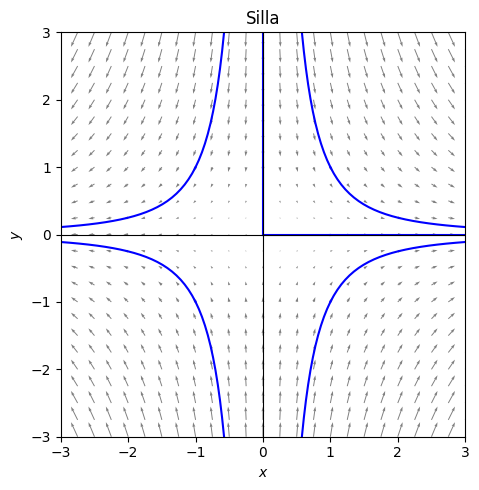
\includegraphics[width=0.4\textwidth]{silla.png}
  \caption{Equilibrio inestable de tipo {\em silla}.}
  \label{fig:silla}
\end{figure}

\begin{figure}[ht]
  \centering
  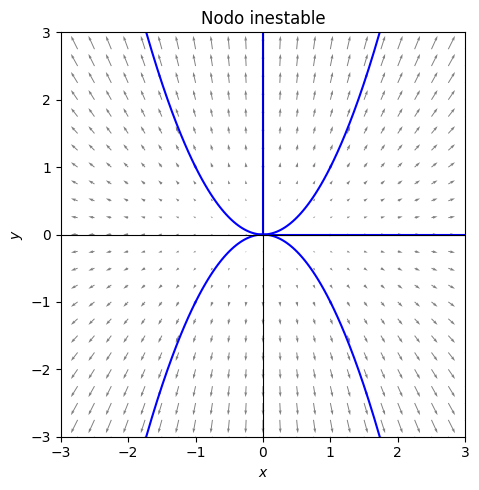
\includegraphics[width=0.4\textwidth]{nodo1.png}
  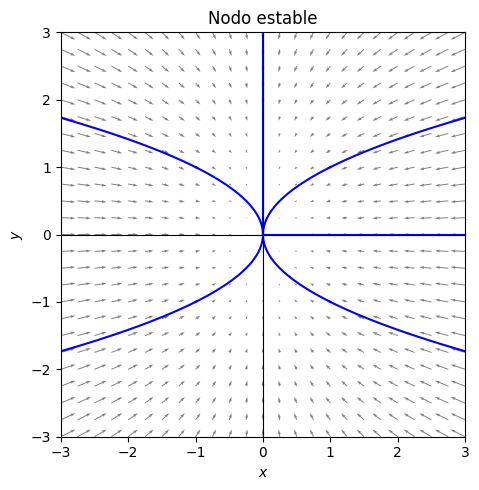
\includegraphics[width=0.4\textwidth]{nodo2.png}
  \caption{Equilibrios de tipo {\em nodo}. A la izquierda inestable y a la derecha asintóticamente estable.}
  \label{fig:nodo}
\end{figure}

\begin{figure}[ht]
  \centering
  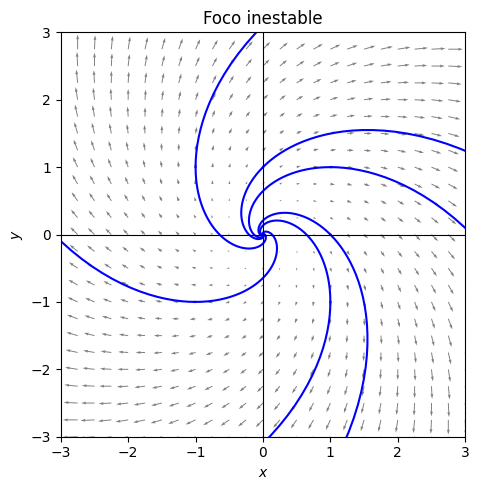
\includegraphics[width=0.4\textwidth]{foco1.png}
  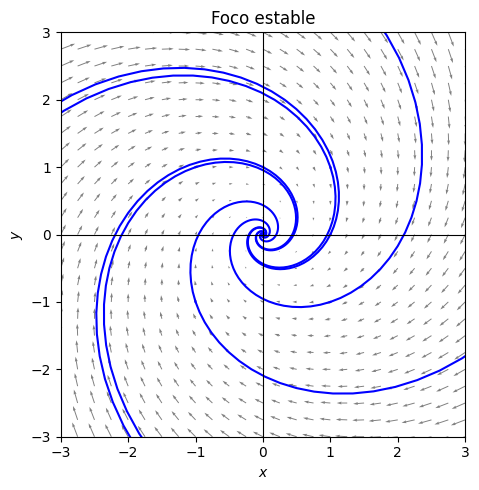
\includegraphics[width=0.4\textwidth]{foco2.png}
  \caption{Equilibrios de tipo {\em foco}. A la izquierda inestable y a la derecha asintóticamente estable.}
  \label{fig:foco}
\end{figure}

\begin{figure}[ht]
  \centering
  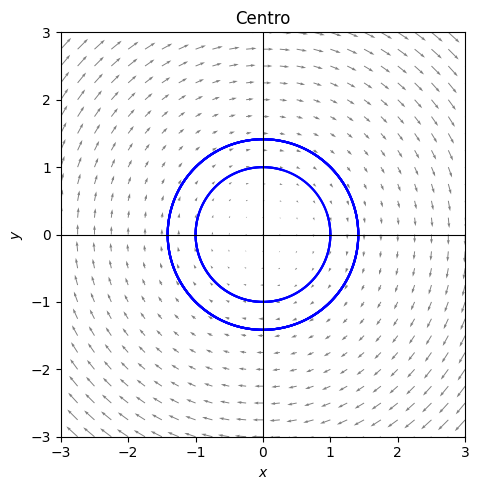
\includegraphics[width=0.4\textwidth]{centro.png}
  \caption{Equilibrio estable de tipo {\em centro}.}
  \label{fig:centro}
\end{figure}

\begin{figure}[ht]
  \centering
  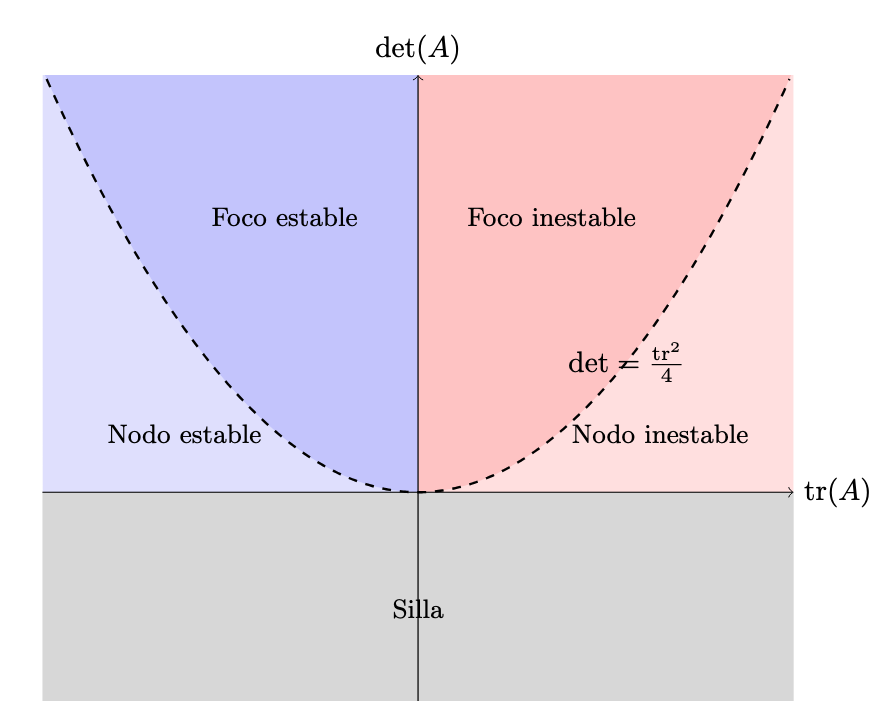
\includegraphics[width=0.4\textwidth]{clasificacion.png}
  \caption{Regiones descriptas en el Teorema \ref{teo.lineal}.}
  \label{fig:clasificacion}
\end{figure}

\section{El Teorema de Hartman-Grobman}

Ahora veremos el enunciado del Teorema de Hartman-Grobman. Empecemos con una definición.
\begin{defi}
Sea $F\colon \R^n\to\R^n$ un campo de clase $C^1$ y sea $\xx^*\in\R^n$ un punto fijo, i.e. $F(\xx^*)=0$.

Decimos que $\xx^*$ es un punto fijo {\em hiperbólico}, si todos los autovalores de la matriz diferencial $DF(\xx^*)$ tienen parte real no nula.
\end{defi}

El Teorema de Hartman-Grobman describe el comportamiento del flujo asociado a $F$ en un entorno de cada punto fijo hiperbólico.
\begin{teo}[Hartman-Grobman]
Sea $F\colon\R^n\to\R^n$ un campo de clase $C^1$ y sea $\xx^*$ un punto fijo hiperbólico de $F$. Entonces existen un entorno $U$ de $\xx^*$, un entorno $W$ de $0$ y un homeomorfismo $\hh\colon U\to W$ con $\hh(\xx^*)=0$ que lleva las trayectorias de
$$
\dot\xx = F(\xx) \quad \text{en las trayectorias de}\quad \dot \yy = DF(\xx^*)\yy
$$
preservando el sentido del tiempo. Es decir, los dos flujos son topológicamente conjugados en un entorno del equilibrio.
\end{teo}

\begin{obs}\label{obs:HG-topologico}
El teorema es \emph{local} (vale en un entorno de $\xx^*$, no en todo $\R^n$) y la conjugación es sólo \emph{topológica}. Esto último no es una limitación de la demostración sino del resultado: el sistema lineal $\dot x = x$, $\dot y = 2y$ y el sistema $\dot x = x$, $\dot y = 2y + x^2$ tienen la misma linealización en el origen, pero no existe ningún cambio de coordenadas de clase $C^2$ (ni, en particular, analítico) que conjugue sus flujos: la relación $\lambda_2 = 2\lambda_1$ entre los autovalores, llamada \emph{resonancia}, lo impide. Sí existe un homeomorfismo, como asegura el teorema (y en este ejemplo hasta un cambio de coordenadas $C^1$, $(x,y)\mapsto(x,\,y-x^2\ln|x|)$, pero no más regular). En la práctica, lo que usamos del teorema es lo siguiente: \emph{cerca de un equilibrio hiperbólico, el diagrama de fases del sistema no lineal se ve como el del sistema lineal}: un sumidero, una fuente o una silla, según los autovalores de $DF(\xx^*)$.
\end{obs}

\begin{proof}
La demostración de este teorema es bastante técnica y elaborada y el interesado puede encontrarla en \cite{Coddington}. Para tener alguna intuición sobre el porqué de la validez de este teorema vamos a desarrollar un argumento puramente formal.

Si realizamos una expansión de Taylor para el campo $F$, obtenemos
$$
F(\xx^*+\yy) = \underbrace{F(\xx^*)}_{0}+ DF(\xx^*)\yy + o(\|\yy\|).
$$
Luego, para $\yy$ pequeño, tenemos
$$
\dot\yy = \frac{d}{dt}(\xx-\xx^*) = \dot\xx = F(\xx) = F(\xx^*+\yy) \sim DF(\xx^*)\yy.
$$
Luego las soluciones de $\dot\xx = F(\xx)$ tienen un comportamiento similar cerca de $\xx^*$ a las de $\dot \yy = DF(\xx^*)\yy$.

Para que el argumento de Taylor sea válido, es necesario que el error sea pequeño y ahí es donde se necesita que $\Re(\lambda)\neq 0$ para todo autovalor $\lambda$ de $DF(\xx^*)$.
\end{proof}

Veamos una aplicación de este resultado.

\begin{ejem}[El péndulo amortiguado]\label{ej:pendulo_amortiguado}
La ecuación para el péndulo amortiguado es
$$
\ddot \theta + 2a\dot\theta + \omega^2 \sin\theta = 0,
$$
donde $\theta$ es el ángulo de desplazamiento respecto de la posición de equilibrio (ver Figura \ref{fig:pendulo}), $a>0$ es el coeficiente de fricción y $\omega^2=g/\ell$, la fuerza de gravedad dividida por la longitud del péndulo.

Llamemos $x_1=\theta$ y $x_2=\dot\theta$, con lo que la ecuación del péndulo se traduce en
\begin{equation}\label{pendulo.amortiguado}
\begin{cases}
&\dot x_1 = x_2\\
&\dot x_2 = -2ax_2 - \omega^2\sin x_1.
\end{cases}
\end{equation}
Los puntos de equilibrio son $x_2=0$, $x_1=k\pi$ con $k\in\Z$. La matriz diferencial del campo $F(x_1, x_2)=(x_2, -\omega^2\sin x_1 - 2ax_2)^t$ es
$$
DF(x_1, x_2) = \begin{bmatrix}
0 & 1\\
-\omega^2\cos x_1 & -2a
\end{bmatrix}
$$

Si $k$ es par, los autovalores de $DF(k\pi, 0)$ son $\lambda_{1,2} = -a\pm\sqrt{a^2-\omega^2}$. Luego, si $\omega\le a$ tenemos que ambos son reales y negativos y el equilibrio es un nodo estable. Por otro lado, si $\omega>a$ los autovalores son complejos conjugados con parte real $-a<0$, con lo que el equilibrio es un foco estable.

Si $k$ es impar, los autovalores de $DF(k\pi, 0)$ son $\lambda_{1,2} = -a\pm\sqrt{a^2+\omega^2}$. Luego ambos son reales y de signos opuestos. Esto implica que el equilibrio es una silla.

El diagrama de fases, para el caso $\omega>a$, está en la Figura \ref{fig:pendulo.amortiguado}.
\end{ejem}

\begin{figure}[ht]
  \centering
  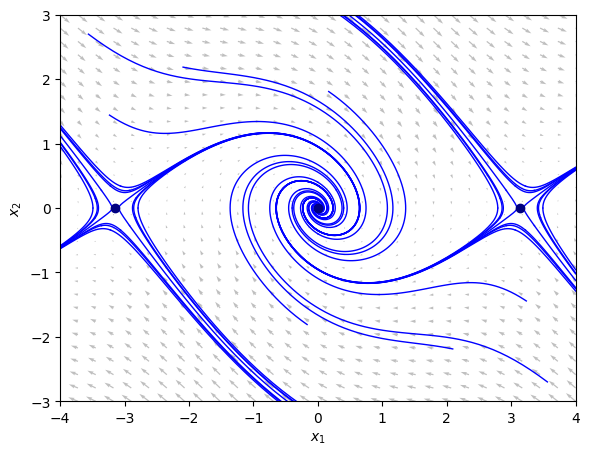
\includegraphics[width=0.6\textwidth]{pendulo-amortiguado.png}
  \caption{Diagrama de fases para \eqref{pendulo.amortiguado}.}
  \label{fig:pendulo.amortiguado}
\end{figure}

\begin{defi}
Un punto de equilibrio $\xx^*$ de un campo $F\in C^1(\R^n; \R^n)$ se dice:
\begin{itemize}
\item una {\em fuente} si todos los autovalores de $DF(\xx^*)$ tienen parte real positiva,
\item un {\em sumidero} si todos los autovalores de $DF(\xx^*)$ tienen parte real negativa,
\item una {\em silla} si $\xx^*$ es hiperbólico y existe al menos un autovalor con parte real positiva y al menos un autovalor con parte real negativa.
\end{itemize}
\end{defi}

Cuando algún autovalor tiene parte real cero, el Teorema de Hartman-Grobman no da información. Y de hecho es fácil construir ejemplos donde el equilibrio sea un centro, una fuente o un sumidero. En efecto, veamos el siguiente ejemplo.

\begin{ejem}[Oscilador armónico perturbado]
Consideremos el sistema
\begin{equation}\label{eq:sinHG}
\begin{cases}
\dot x_1 = x_2 + \lambda x_1(x_1^2+x_2^2)\\
\dot x_2 = -x_1 + \lambda x_2(x_1^2+x_2^2),
\end{cases}
\end{equation}
donde $\lambda\in\R$ es un parámetro. Este sistema describe la dinámica de un oscilador armónico perturbado.

Para todo valor de $\lambda\in\R$, $\xx^*=(0,0)^t$ resulta ser un punto de equilibrio. La matriz diferencial del campo $F(x_1, x_2)=(x_2 + \lambda x_1(x_1^2+x_2^2),  -x_1 + \lambda x_2(x_1^2+x_2^2))^t$ evaluada en el origen es
$$
DF(0,0) = \begin{bmatrix}
0 & 1\\
-1 & 0
\end{bmatrix}.
$$
Sus autovalores son $\lambda_{1, 2} = \pm i$, luego el origen no es hiperbólico.

Para analizar la estabilidad del origen debemos argumentar de otra manera. En este caso resulta conveniente mirar al punto $(x_1, x_2)$ en coordenadas polares
$$
x_1 = r\cos\theta\quad \text{y} \quad x_2=r\sin\theta.
$$
Es fácil ver que en términos de $r$ y $\theta$ el sistema queda
$$
\dot r = \lambda r^3 \quad \text{y}\quad \dot\theta = -1
$$
La ecuación para $\theta$ dice que las trayectorias rotan monótonamente en el sentido de las agujas del reloj y la ecuación para $r$ dice que el origen resulta ser asintóticamente estable si $\lambda<0$, un centro si $\lambda=0$ e inestable para $\lambda>0$.
\end{ejem}

\begin{figure}[ht]
  \centering
  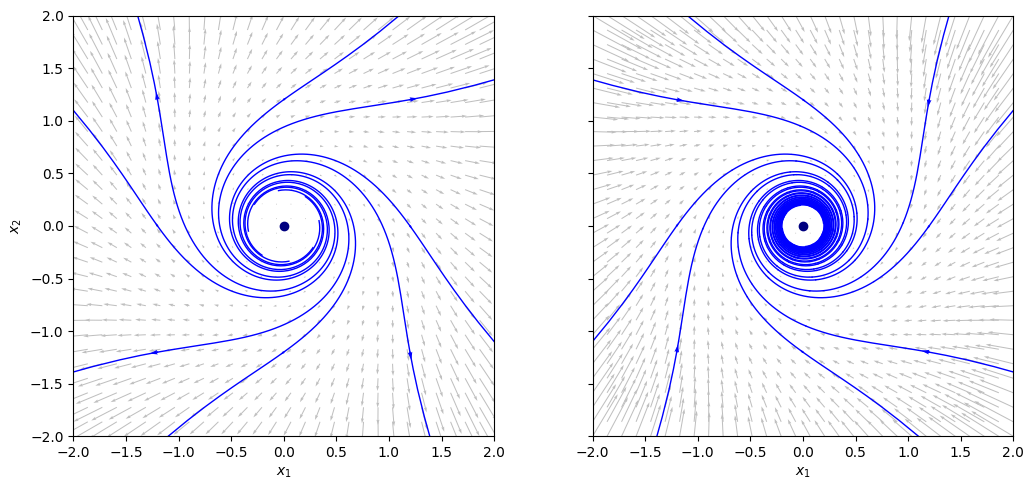
\includegraphics[width=0.6\textwidth]{sinHG.png}
  \caption{Diagrama de fases para \eqref{eq:sinHG}. A la izquierda para $\lambda>0$ y a la derecha para $\lambda<0$.}
  \label{fig:sinHG}
\end{figure}



\section{Volvemos a los modelos poblacionales}\label{sec:HG-modelos}

Con el Teorema de Hartman--Grobman y la clasificación de los sistemas lineales en el plano (Teorema \ref{teo.lineal}) podemos justificar casi todo lo que en el Capítulo \ref{cap1} sólo pudimos observar en las simulaciones. La receta es siempre la misma: calcular la matriz diferencial del campo en cada equilibrio, sus autovalores (o, en dimensión dos, su traza y su determinante), verificar que el equilibrio es hiperbólico y leer el comportamiento en el Teorema \ref{teo.lineal}.

\subsection*{Lotka--Volterra clásico}

Para el sistema \eqref{LV1}, $F(h,p) = (\rho h(1-p), -\frac1\rho p(1-h))^t$ y
$$
DF(h,p) =
\begin{bmatrix}
\rho(1-p) & -\rho h\\[4pt]
\dfrac{1}{\rho}p & -\dfrac{1}{\rho}(1-h)
\end{bmatrix},
\
DF(0,0) = \begin{bmatrix} \rho & 0\\ 0 & -1/\rho\end{bmatrix},
\
DF(1,1) = \begin{bmatrix} 0 & -\rho\\ 1/\rho & 0\end{bmatrix}.
$$
En el origen los autovalores son $\rho>0$ y $-1/\rho<0$: es hiperbólico y es una \emph{silla}, con el eje $h$ como dirección inestable y el eje $p$ como dirección estable, exactamente como observamos. En $(1,1)$ los autovalores son $\pm i$: el equilibrio \emph{no es hiperbólico} y el teorema no dice nada. Es una suerte que en la Sección \ref{sec:LV1-analisis} hayamos encontrado la cantidad conservada $\Hc$: ella es la que decide que $(1,1)$ es un centro. Este es un buen ejemplo de que la linealización no siempre alcanza.

\subsection*{Lotka--Volterra con capacidad de carga}

Para el sistema \eqref{LV2}, la matriz diferencial es
$$
DF(h,p) =
\begin{bmatrix}
\rho\left(1-\dfrac{2h}{k}-p\right) & -\rho h\\[6pt]
\dfrac{p}{\rho} & -\dfrac{1-h}{\rho}
\end{bmatrix},
$$
y evaluándola en los tres equilibrios,
$$
DF(0,0)=\begin{bmatrix} \rho & 0\\ 0 & -1/\rho\end{bmatrix},\
DF(k,0)=\begin{bmatrix} -\rho & -k\rho\\ 0 & (k-1)/\rho\end{bmatrix},\
DF\Bigl(1,1-\tfrac1k\Bigr)=\begin{bmatrix} -\rho/k & -\rho\\[4pt] \dfrac{k-1}{k\rho} & 0\end{bmatrix}.
$$
\begin{itemize}
\item $(0,0)$ es siempre una silla (autovalores $\rho$ y $-1/\rho$).
\item $(k,0)$ tiene autovalores $-\rho$ y $(k-1)/\rho$. Si $k<1$ ambos son negativos y es un \emph{nodo estable}: los predadores se extinguen y los herbívoros van a la capacidad de carga, como vimos en la Figura \ref{fig:LVk<1}. Si $k>1$ es una silla. Si $k=1$ tiene un autovalor nulo, no es hiperbólico, y el teorema no se aplica: es el caso ``lento'' de la Figura \ref{fig:LVk=1}.
\item En el equilibrio de coexistencia (que existe si $k>1$), $\tr DF = -\rho/k<0$ y $\det DF = (k-1)/k>0$, así que es siempre \emph{asintóticamente estable}. Los autovalores son
$$
\lambda_\pm = \frac{-\rho\pm\sqrt{\rho^2-4k(k-1)}}{2k},
$$
reales si $\rho^2\ge 4k(k-1)$ (nodo estable, Figura \ref{fig:LVk>1-1}) y complejos con parte real $-\rho/(2k)$ si $\rho^2<4k(k-1)$ (foco estable, Figura \ref{fig:LVk>1-2}).
\end{itemize}
La curva $\rho^2 = 4k(k-1)$ en el plano $(k,\rho)$ es la que separa el acercamiento monótono del oscilatorio, que era la pregunta que había quedado abierta. Notemos que, para $k$ grande (capacidad de carga grande, es decir, cerca del modelo clásico), casi siempre estamos en el caso oscilatorio, y la parte real $-\rho/(2k)$ tiende a cero: las oscilaciones se amortiguan cada vez más lentamente, y en el límite $k\to\infty$ recuperamos las órbitas cerradas de \eqref{LV1}.

\subsection*{El modelo de bacterias y el umbral $k_c$}

Para el sistema \eqref{bacteria2}, la matriz diferencial del campo evaluada en el punto fijo $(1,1)$ es (ejercicio)
$$
DF(1,1) =
\begin{bmatrix}
\dfrac{k-2-\beta}{k(1+\beta)} & -1 + \dfrac{1}{k}\\[6pt]
\dfrac{\beta\gamma}{1+\beta} & 0
\end{bmatrix}.
$$
Recordemos que, para una matriz $2\times 2$, ambos autovalores tienen parte real negativa si y sólo si $\det>0$ y $\tr<0$. En este caso
$$
\det DF(1,1) = \frac{(k-1)\beta\gamma}{k(1+\beta)}>0 \iff k>1,
\
\tr DF(1,1) = \frac{k-2-\beta}{k(1+\beta)}<0 \iff k<2+\beta.
$$
Luego, si $1<k<2+\beta$, el equilibrio $(1,1)$ es asintóticamente estable (Figura \ref{fig:bacteria1}), y si $k>2+\beta$ es inestable (una fuente). Esto confirma que el umbral observado en las simulaciones es
$$
k_c = 2+\beta,
$$
el valor para el cual el equilibrio pasa por el vértice de la parábola nulclina. En $k=k_c$ la traza se anula, los autovalores son imaginarios puros y el equilibrio no es hiperbólico. Lo que el teorema no explica es por qué, al perder estabilidad el equilibrio, aparece un ciclo límite: para eso hay que esperar al Capítulo \ref{cap:bifurcaciones}.

\begin{volvemos}{la epidemia}
Para el modelo SIR \eqref{SIR} en las variables $(s,i)$, $F(s,i) = (-\beta si, \beta si-\gamma i)^t$ y en un equilibrio $(s^*,0)$
$$
DF(s^*,0) = \begin{bmatrix} 0 & -\beta s^*\\ 0 & \beta s^*-\gamma\end{bmatrix},
$$
cuyos autovalores son $0$ y $\beta s^*-\gamma = \gamma(R_0 s^*-1)$. El autovalor nulo era previsible: hay un segmento entero de equilibrios, y a lo largo de él el campo no ``empuja''. Ningún equilibrio del SIR es hiperbólico y el teorema de Hartman--Grobman no se aplica. Lo que sí nos dice la linealización es el signo del otro autovalor, que reproduce el umbral que encontramos a mano: $R_0 s^*<1$ (dirección atractora transversal al segmento) o $R_0 s^*>1$ (dirección repulsora). El análisis directo del Capítulo \ref{cap:flujo} sigue siendo el que decide la estabilidad.
\end{volvemos}

\begin{volvemos}{el circuito}
Para el sistema de van der Pol \eqref{eq:vdP-sistema}, $F(x,y) = (y, -x-\lambda(x^2-1)y)^t$ y
$$
DF(0,0) = \begin{bmatrix} 0 & 1\\ -1 & \lambda\end{bmatrix},\qquad \tr = \lambda,\quad \det = 1,
$$
con autovalores $\frac12\bigl(\lambda\pm\sqrt{\lambda^2-4}\bigr)$. Para todo $\lambda\neq 0$ el origen es \emph{hiperbólico} y el teorema se aplica: si $\lambda>0$ es un foco inestable (para $0<\lambda<2$) o un nodo inestable (para $\lambda\ge 2$), y si $\lambda<0$ es un foco o un nodo estable. Queda demostrado que, para $\lambda>0$, el circuito se enciende: el reposo es inestable. Sólo en $\lambda=0$ (el oscilador armónico puro) el origen es un centro no hiperbólico, y el sistema \eqref{eq:vdP-sistema} es, en ese caso, exactamente lineal.
\end{volvemos}

\chapter{Sistemas conservativos y funciones de Lyapunov}\label{cap:lyapunov}

En este capítulo empezamos estudiando sistemas mecánicos que introducimos en el Capítulo \ref{sec:sistemas-mecanicos} y explotamos el hecho de que muchos de esos sistemas tienen cantidades conservadas (la energía) para analizar la estabilidad de los equilibrios. Luego vemos como esa idea puede ser extendida por el uso de {\em funciones de Lyapunov} que fueran introducidos por A. M. Lyapunov en su tesis doctoral de 1892 \cite{Lyapunov}.

\section{Sistemas conservativos}

De acuerdo con la segunda ley de Newton, una partícula sometida a la acción de una fuerza $F$ obedece la ecuación
$$
F = m \ab,
$$
donde $m>0$ es la masa de la partícula y $\ab$ su aceleración.

Si la posición de la partícula está dada por $\xx(t)\in\R^n$, la velocidad $\vv(t)$ y la aceleración $\ab(t)$ se definen como
$$
\dot\xx = \vv,
\qquad
\ddot\xx = \dot\vv = \ab.
$$
La partícula tiene asociada una \emph{energía cinética} $E_c$, definida por
$$
E_c = \frac12 m |\vv|^2 = \frac12 m |\dot\xx|^2.
$$

En muchos contextos físicos, la fuerza $F$ deriva de un potencial escalar $U\colon \R^n \to \R$, es decir,
$$
F = -\nabla U.
$$
En este caso, se define la \emph{energía potencial} de la partícula como
$$
E_p = U(\xx).
$$

La suma de la energía cinética y la energía potencial,
$$
E = E_c + E_p = \frac12 m |\dot\xx|^2 + U(\xx),
$$
se denomina \emph{energía mecánica total} del sistema.

Un sistema de este tipo se llama \emph{conservativo}, ya que la energía mecánica se conserva a lo largo del movimiento. En efecto, derivando respecto del tiempo se obtiene
$$
\frac{dE}{dt}
= m \dot\xx\cdot\ddot\xx + \nabla U(\xx)\cdot \dot\xx
= \dot\xx\cdot\bigl(m\ddot\xx + \nabla U(\xx)\bigr).
$$
Usando la ecuación de movimiento $m\ddot\xx = F(\xx) = -\nabla U(\xx)$, se concluye que
$$
\frac{dE}{dt} = 0,
$$
y por lo tanto la energía total $E$ es constante a lo largo de las trayectorias.

Desde el punto de vista dinámico, el movimiento de una partícula en un campo de fuerzas conservativo puede formularse como un sistema de ecuaciones diferenciales de primer orden en el espacio de fases $(\xx,\vv)\in \R^n\times\R^n$, dado por
$$
\begin{cases}
\dot\xx = \vv, \\
\dot\vv = -\dfrac{1}{m}\nabla U(\xx).
\end{cases}
$$
En este marco, las trayectorias del sistema quedan confinadas a los conjuntos de nivel de la energía total $E$, lo que impone fuertes restricciones sobre la dinámica y constituye una de las características fundamentales de los sistemas conservativos.

\subsection{El caso unidimensional}

Cuando $n=1$, la energía total queda definida como 
$$
E = \frac12 m|\dot x|^2 + U(x),
$$
con $U\colon\R\to\R$ y luego, llamando $y=\dot x$, obtenemos $E\colon \R^2\to\R$, $E(x, y)=\frac{m}{2} y^2 + U(x)$.

\begin{ejem}[El péndulo]\label{ej:pendulo}
En la sección \ref{sec:pendulo} estudiamos el caso del péndulo simple
$$
\ddot \theta + \omega^2 \sin\theta = 0,\quad \omega^2 = \frac{g}{\ell}.
$$
Llamando $x=\theta$, $y=\dot\theta$, reescribimos el problema como
$$
\begin{cases}
\dot x = y\\
\dot y = -\omega^2\sin x
\end{cases}
$$

Luego, si definimos $U(x) = \omega^2(1-\cos x)$, tenemos que $U'(x) = \omega^2\sin x$, de donde 
$$
E(x, y) = \frac12 y^2 + U(x) = \frac12 y^2 + \omega^2(1-\cos x)
$$
resulta constante sobre las trayectorias del sistema. En la Figura \ref{fig:energia_pendulo} están graficadas algunas curvas de nivel de $E$ y en la Figura \ref{fig:pendulo_potencial} están graficados juntos la función potencial con el diagrama de fases.
\end{ejem}

\begin{figure}[ht]
  \centering
  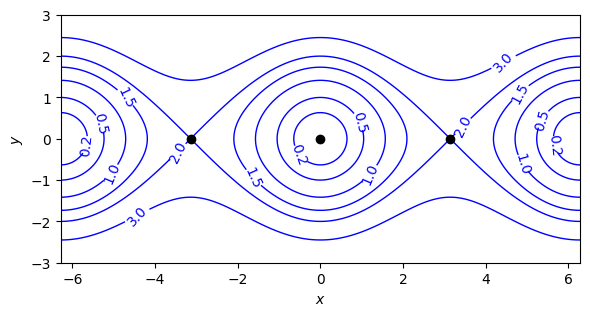
\includegraphics[width=0.6\textwidth]{energia_pendulo.png}
  \caption{Curvas de nivel para la energía asociada el péndulo simple.}
  \label{fig:energia_pendulo}
\end{figure}

\begin{figure}[ht]
  \centering
  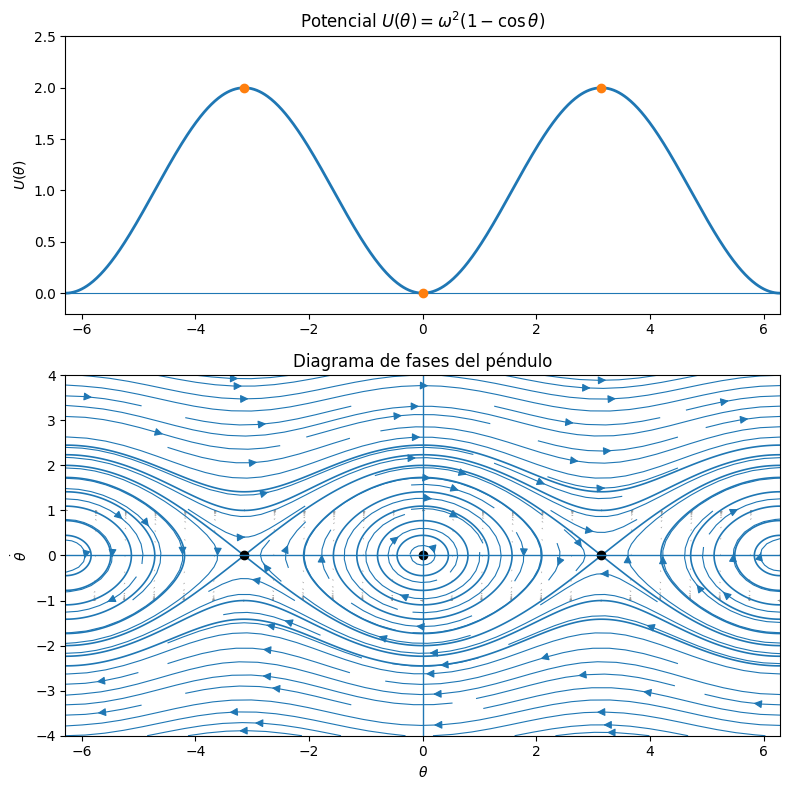
\includegraphics[width=0.6\textwidth]{pendulo_potencial.png}
  \caption{Función potencial y trayectorias para el péndulo simple.}
  \label{fig:pendulo_potencial}
\end{figure}

Observemos que en todo sistema de la forma
$$
\begin{cases}
\dot x = y\\
\dot y = -U'(x)
\end{cases}
$$
tendremos que la energía $E(x, y) = \frac12 y^2 + U(x)$ será conservada por las trayectorias, con lo que cada trayectoria estará contenida en una curva de nivel de $E$. Por otro lado, cuando la trayectoria se encuentre en el semiplano superior $\{y>0\}$, tendremos $\dot x>0$ con lo cual la trayectoria se moverá de izquierda a derecha, mientras que en semiplano inferior, $\{y<0\}$, la trayectoria se moverá de derecha a izquierda.

Por otro lado, los equilibrios del sistema serán de la forma $(x^*, 0)$ donde $U'(x^*)=0$. Es decir, $x^*$ es un punto crítico del potencial $U$.

Finalmente observemos que si una trayectoria $(x(t), y(t))$ verifica que para algún $t_0$ se tiene que $y(t_0)=0$ y llamamos $\bar x = x(t_0)$ entonces
$$
U(\bar x) = E(x(t_0), y(t_0)) = E(x(t), y(t)) = \frac12 y^2(t) + U(x(t))\ge U(x(t)).
$$
Es decir que a lo largo de toda la trayectoria, la misma no escapa el {\em pozo de potencial} $U(x)\le U(\bar x)$ y sólo alcanza ese nivel de potencial si simultáneamente se tiene que $y=0$. Ver Figura \ref{fig:potencial}.
\begin{figure}[ht]
  \centering
  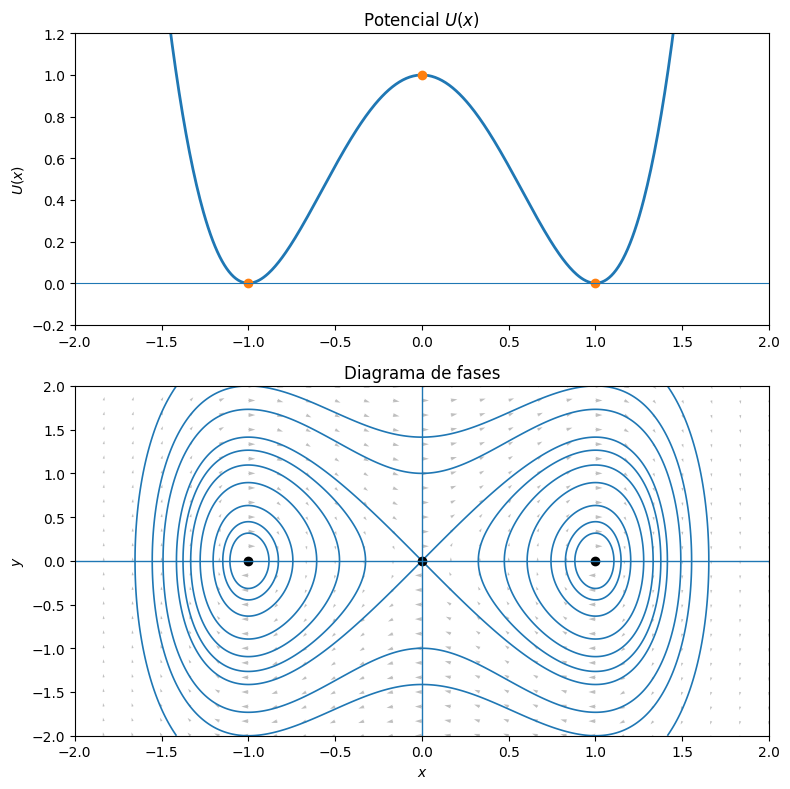
\includegraphics[width=0.6\textwidth]{potencial.png}
  \caption{Función potencial y diagrama de fases asociado.}
  \label{fig:potencial}
\end{figure}


\section{Funciones de Lyapunov}

Tomando la idea de la sección anterior, en su tesis doctoral de 1892, A. M. Lyapunov introduce lo que hoy llamamos {\em funciones de Lyapunov} para estudiar la estabilidad de puntos de equilibrio.

\begin{defi}[Función de Lyapunov]
Sea $\xx^*\in\R^n$ un punto de equilibrio de la ecuación $\dot\xx = F(\xx)$. Sea $V\colon U\subset\R^n\to\R$ una función de clase $C^1$ donde $U$ es un entorno de $\xx^*$. Decimos que $V$ es una función de Lyapunov para $\xx^*$ si
\begin{enumerate}
\item $V$ tiene un mínimo estricto en $\xx^*$: $V(\xx)> V(\xx^*)$ para todo $\xx\in U$, $\xx\neq \xx^*$;
\item $V$ no crece a lo largo de las soluciones: para todo $\xx\in U$,
$$
\dot V(\xx) = \frac{d}{dt}V(\phi_t(\xx))\Big|_{t=0}\le 0,
$$
donde $\phi_t$ es el flujo asociado a la ecuación.
\end{enumerate}
Cuando en la desigualdad anterior se reemplaza $\le$ por $<$ para todo $\xx\neq\xx^*$, se dice que $V$ es una función de Lyapunov \emph{estricta}.
\end{defi}

\begin{teo}[Lyapunov]\label{teo:lyapunov}
Sea $\xx^*$ un equilibrio de $\dot\xx = F(\xx)$. Si existe una función de Lyapunov en un entorno de $\xx^*$, entonces el equilibrio es estable. Si existe una función de Lyapunov estricta, entonces el equilibrio es asintóticamente estable.
\end{teo}

La idea de la demostración es simple (los detalles pueden verse en \cite{Hirsch-Smale}). Como $V$ tiene un mínimo estricto en $\xx^*$, los conjuntos de nivel $\{V< c\}$ para $c$ apenas mayor que $V(\xx^*)$ son entornos chicos de $\xx^*$. Como $V$ no crece sobre las soluciones, una trayectoria que empieza en $\{V<c\}$ no puede salir de ahí: eso es la estabilidad. Si además $V$ decrece estrictamente, la trayectoria tiene que ir bajando de nivel hasta el mínimo: eso es la estabilidad asintótica.

En los ejemplos aparece con frecuencia una situación intermedia: $\dot V\le 0$, pero $\dot V$ se anula en algunos puntos distintos del equilibrio (típicamente, sobre una curva), de modo que $V$ no es estricta. El siguiente refinamiento resuelve esos casos.

\begin{teo}[Principio de invariancia de LaSalle]\label{teo:lasalle}
Sea $V$ una función de Lyapunov para $\xx^*$ en un entorno $U$, y sea $Z = \{\xx\in U\colon \dot V(\xx) = 0\}$. Si la única trayectoria completa contenida en $Z$ es el equilibrio $\xx^*$, entonces $\xx^*$ es asintóticamente estable.
\end{teo}

Dicho de otro modo: no importa que $\dot V$ se anule en algunos puntos, siempre que las trayectorias no puedan \emph{quedarse} en esos puntos. Una demostración puede verse en \cite{Hirsch-Smale-Devaney}.

Un hecho fundamental, es que se puede calcular $\dot V(\xx)$ sin la necesidad de calcular el flujo de la EDO. En efecto, usando la regla de la cadena,
\begin{align*}
\dot V(\xx) &= \frac{d}{dt}V(\phi_t(\xx))|_{t=0} = (\nabla V(\phi_t(\xx))\cdot \dot\phi_t(\xx))|_{t=0}\\
& = (\nabla V(\phi_t(\xx))\cdot F(\phi_t(\xx)))|_{t=0} = \nabla V(\xx)\cdot F(\xx)
\end{align*}

La dificultad en aplicar el método de Lyapunov consiste justamente en encontrar una función de Lyapunov para una EDO dada. Sin embargo hay ciertas situaciones en donde esto es relativamente simple. Veamos algunos ejemplos.

\begin{ejem}[Sistemas conservativos]\label{ej:sistema_conservativo}
Como vimos en la sección anterior, si tenemos un sistema de la forma
$$
\begin{cases}
\dot \xx = \yy\\
\dot \yy = -\nabla U(\xx)
\end{cases}
$$
definido en $\R^{2n}$, el mismo tiene una energía mecánica total dada por $E(\xx, \yy) = \frac12 |\yy|^2 + U(\xx)$. Esta energía verifica que $\dot E=0$. Luego si $\xx^*$ es un mínimo de $U$ sigue que $E$ es una función de Lyapunov para el punto crítico $(\xx^*, 0)$ y por ende el mismo resulta estable.
\end{ejem}

 
\begin{ejem}[Sistemas Hamiltonianos]
Una generalización del ejemplo anterior son los llamados {\em sistemas Hamiltonianos}. Sea $H\colon \R^{2n}\to \R$ una función de clase $C^1$ (la función $H$ se la llama el {\em Hamiltoniano}) y consideramos el sistema
$$
\begin{cases}
\dot \qq = H_{\pp}(\qq, \pp)\\
\dot \pp = -H_{\qq}(\qq, \pp),
\end{cases}
$$
donde $\pp, \qq\in \R^n$, $\pp = (p_1,\dots,p_n)^t$, $\qq=(q_1,\dots,q_n)^t$, $H_{\pp} = (\partial_{p_1} H,\dots, \partial_{p_n}H)^t$ y $H_{\qq} = (\partial_{q_1} H,\dots, \partial_{q_n}H)^t$

Observemos que $\dot H(\pp, \qq) = H_{\pp}(\pp, \qq)\cdot \dot\pp + H_{\qq}(\pp, \qq)\cdot \dot\qq = 0$. Es decir, el Hamiltoniano es constante a lo largo de las trayectorias del sistema.

Ahora, $(\pp^*, \qq^*)$ es un punto de equilibrio para el sistema si y sólo si es un punto crítico para el Hamiltoniano $H$ y si es un mínimo local para $H$, entonces $H$ resulta ser una función de Lyapunov para $(\pp^*, \qq^*)$. Luego, todo mínimo local de $H$ es un punto de equilibrio estable para el sistema.

Observemos que un sistema Hamiltoniano es una generalización de un sistema conservativo. Basta tomar a la energía total $E$ como Hamiltoniano.
\end{ejem}


\begin{ejem}[Péndulo y péndulo amortiguado]
Un caso importante que ya hemos estudiado en diversas oportunidades es el del péndulo (Secciones \ref{sec:pendulo} y \ref{sec:pendulo_amortiguado} y Ejemplos \ref{ej:pendulo_amortiguado} y \ref{ej:pendulo}). 

Para el péndulo simple, el sistema a analizar es
$$
\begin{cases}
\dot x = y\\
\dot y = -\omega^2\sin x.
\end{cases}
$$
De acuerdo a lo discutido en el Ejemplo \ref{ej:sistema_conservativo}, la energía total 
$$
E(x, y) = \frac12 y^2 + \omega^2(1-\cos x)
$$
resulta ser una función de Lyapunov para los puntos estacionarios de la forma $(x^*, 0)$ con $x^*$ mínimos de la función potencial $U(x) = \omega^2(1-\cos x)$. Por ende estos resultan estables. Ver Figura \ref{fig:pendulo_potencial}.

El péndulo amortiguado es
$$
\begin{cases}
\dot x = y\\
\dot y = -\omega^2\sin x - 2a y.
\end{cases}
$$
En este caso, la amortiguación hace que el péndulo vaya perdiendo energía mecánica, lo que hace suponer que la misma función de energía pueda funcionar como función de Lyapunov. Efectivamente,
$$
\dot E = y \dot y + \omega^2\sin x\dot x = y(-\omega^2\sin x - 2a y) + \omega^2 \sin x\ y = -2ay^2.
$$
Luego $E$ es una función de Lyapunov para los equilibrios $(2k\pi,0)$, que son mínimos de $E$, y estos resultan estables. Pero $\dot E = -2ay^2$ no es estrictamente negativa: se anula sobre todo el eje $y=0$. Acá interviene el principio de LaSalle: una trayectoria que se mantuviera en $\{y=0\}$ tendría $\dot x = y = 0$, es decir $x$ constante, y entonces $\dot y = -\omega^2\sin x = 0$, lo que la obliga a ser un equilibrio. Luego los equilibrios $(2k\pi,0)$ son asintóticamente estables, lo que coincide con lo que obtuvimos por linealización en el Ejemplo \ref{ej:pendulo_amortiguado}. La ventaja del argumento de energía es que además nos dice cuál es la cuenca de atracción: al menos todo el pozo de potencial $\{E<2\omega^2\}$ alrededor de cada mínimo.
\end{ejem}

\begin{volvemos}{el circuito}
Ya sabemos, por el Capítulo \ref{cap:HG}, que el origen del sistema de van der Pol \eqref{eq:vdP-sistema} es inestable para $\lambda>0$ y asintóticamente estable para $\lambda<0$. Veamos qué agrega el método de Lyapunov. La ``energía'' $V(x, y) = \frac12(x^2+y^2)$ tiene un mínimo estricto en el origen y, como calculamos en la Sección \ref{sec:energia-herramienta},
$$
\dot V = -\lambda (x^2-1)y^2.
$$
Si $\lambda<0$, entonces $\dot V\le 0$ en la franja $|x|<1$, con igualdad sólo sobre $y=0$; por el principio de LaSalle (una trayectoria contenida en $y=0$ es un equilibrio, como en el péndulo), el origen es asintóticamente estable, y además toda trayectoria que empiece en el disco $V<1/2$ converge a él. Para $\lambda>0$, $V$ crece estrictamente sobre toda trayectoria de la franja que no sea el equilibrio, y esto muestra que las trayectorias que empiezan cerca del origen se alejan hasta salir de cualquier disco de radio menor que $1$: el origen es inestable, ahora con una estimación de \emph{cuánto} se aleja la corriente antes de que la fricción no lineal empiece a frenarla. Ver Figura \ref{fig:vanderPol}.
\end{volvemos}

\begin{volvemos}{la epidemia}
El modelo SIR tiene una cantidad monótona muy natural: el número de infectados. En la región $s<1/R_0$, $\dot i = (\beta s-\gamma)i<0$ siempre que $i>0$, y $i$ decrece hacia $0$. No es una función de Lyapunov en el sentido estricto de la definición (se anula sobre todo el segmento de equilibrios, no sólo en uno de ellos), pero cumple el mismo papel: es el argumento de monotonía con el que en el Capítulo \ref{cap:flujo} probamos la estabilidad de los equilibrios $(s^*,0)$ con $s^*<1/R_0$.
\end{volvemos}

\begin{obs}[Lotka--Volterra revisitado]
La cantidad conservada $\Hc$ de \eqref{eq:LV1-integral} es una función de Lyapunov (no estricta) para el equilibrio $(1,1)$ de \eqref{LV1}: tiene un mínimo estricto allí y $\dot\Hc = 0$. El Teorema \ref{teo:lyapunov} da la estabilidad que ya conocíamos. Más interesante es el modelo con capacidad de carga \eqref{LV2}: en los ejercicios se propone verificar que, si $p^* = 1-1/k$, la función
$$
V(h,p) = (h-\ln h) + \rho^2 (p - p^*\ln p)
$$
verifica $\dot V = -\frac{\rho}{k}(h-1)^2\le 0$. Por el principio de LaSalle, el equilibrio de coexistencia no sólo es asintóticamente estable (lo que ya sabíamos por linealización) sino que \emph{atrae a todas las trayectorias con $h(0),p(0)>0$}, algo que la linealización, que es local, nunca podría decir. Esto es exactamente lo que mostraban las simulaciones del Capítulo \ref{cap1}.
\end{obs}

\begin{figure}[ht]
  \centering
  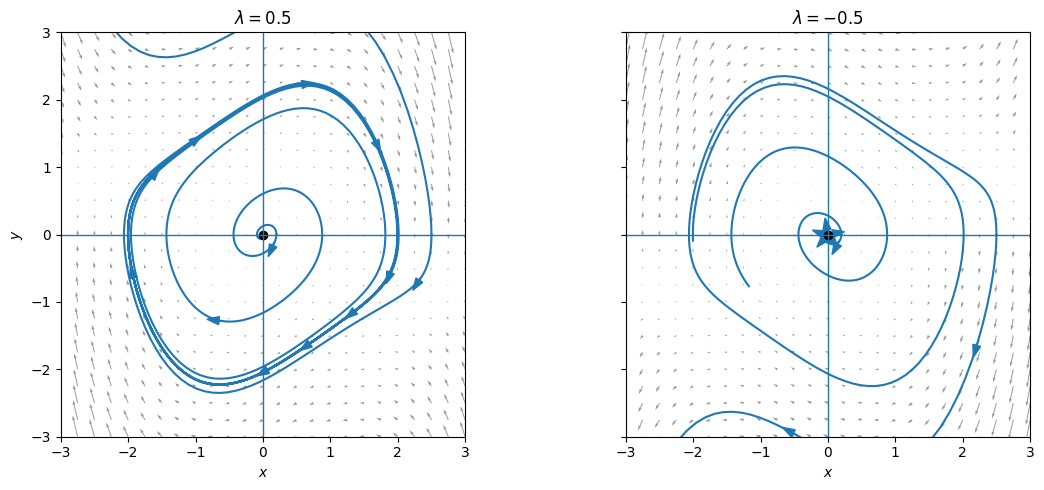
\includegraphics[width=0.6\textwidth]{vanderPol.png}
  \caption{Diagrama de fases para el oscilador de van der Pol \eqref{eq:vdP-sistema}. A la izquierda, $\lambda=0.5$: el origen es inestable y las trayectorias convergen a un ciclo límite. A la derecha, $\lambda=-0.5$: el origen es asintóticamente estable; existe también un ciclo límite inestable (el mismo ciclo recorrido con el tiempo invertido) que separa las trayectorias que convergen al origen de las que escapan.}
  \label{fig:vanderPol}
\end{figure}




\chapter{Dinámica global en dimensión dos}\label{cap:global}

En este capítulo introducimos algunos conceptos generales relacionados con el comportamiento asintótico de soluciones de ecuaciones diferenciales ordinarias. Nuestro objetivo es, luego, dar una descripción global de dicho comportamiento en dimensión dos, donde se dispone de una herramienta fundamental: el Teorema de Poincaré--Bendixon.

\section{\texorpdfstring{$\alpha$ y $\omega$}{alpha y omega} límites}

Dada una ecuación diferencial ordinaria
\[
\dot\xx = F(\xx),
\]
una pregunta fundamental es la siguiente: ¿podemos determinar, para una trayectoria dada $\phi_t(\xx)$, de dónde proviene y hacia dónde va? Es decir, queremos caracterizar todos sus posibles pasados y todos sus posibles futuros. Esta es precisamente la idea detrás de los conjuntos $\alpha$-límite y $\omega$-límite. Recordemos que $\alpha$ es la primera letra del alfabeto griego y $\omega$ la última.

\begin{defi}
Sea $F\in C^1(\R^n;\R^n)$ un campo tal que el flujo asociado $\phi_t$ está globalmente definido. Dado $\xx\in\R^n$, definimos el $\omega$-límite de $\xx$ como el conjunto
\[
L_\omega(\xx) = \{\yy\in\R^n\colon \exists\, t_k\to\infty \text{ tal que } \phi_{t_k}(\xx)\to \yy \text{ cuando } k\to\infty\}.
\]
Análogamente, definimos el $\alpha$-límite de $\xx$ como
\[
L_\alpha(\xx) = \{\yy\in\R^n\colon \exists\, t_k\to-\infty \text{ tal que } \phi_{t_k}(\xx)\to \yy \text{ cuando } k\to\infty\}.
\]
\end{defi}

Un ejemplo simple de conjunto $\omega$-límite está dado por los puntos de equilibrio asintóticamente estables. Para formalizar esta idea introducimos la siguiente definición.

\begin{defi}
Sea $F\in C^1(\R^n;\R^n)$ un campo tal que el flujo asociado $\phi_t$ está globalmente definido. Sea $\xx^*$ un equilibrio asintóticamente estable. Definimos su {\em cuenca de atracción} como el conjunto
\[
B(\xx^*) = \{\xx\in\R^n\colon \phi_t(\xx)\to\xx^* \text{ cuando } t\to\infty\}.
\]
\end{defi}

Es inmediato verificar que $L_\omega(\xx)=\{\xx^*\}$ para todo $\xx\in B(\xx^*)$.

Una propiedad fundamental de los conjuntos $\omega$-límite (y análogamente de los conjuntos $\alpha$-límite) es su invariancia por el flujo.

\begin{prop}
Sea $F\in C^1(\R^n;\R^n)$ un campo tal que el flujo asociado $\phi_t$ está globalmente definido. Sea $\xx\in\R^n$ y $\yy\in L_\omega(\xx)$. Entonces
\[
\phi_t(\yy)\in L_\omega(\xx) \quad \text{para todo } t\in\R,
\]
es decir, $\phi_t(L_\omega(\xx))\subset L_\omega(\xx)$.
\end{prop}

\begin{proof}
Sea $\yy\in L_\omega(\xx)$ y sea $t\in\R$. Definimos $\zz=\phi_t(\yy)$. Por definición de conjunto $\omega$-límite, existe una sucesión $t_k\to\infty$ tal que $\phi_{t_k}(\xx)\to\yy$ cuando $k\to\infty$.

Como el flujo es continuo, se tiene
\[
\phi_{t+t_k}(\xx)=\phi_t(\phi_{t_k}(\xx))\to\phi_t(\yy)=\zz,
\]
lo que prueba la afirmación.
\end{proof}

\section{El Teorema de Poincaré--Bendixon}

En general, obtener una descripción completa del conjunto $\omega$-límite de una ecuación diferencial puede ser una tarea extremadamente compleja. Un ejemplo paradigmático es el atractor de Lorenz, que describe el $\omega$-límite de ciertas trayectorias de un sistema caótico (ver Figura~\ref{fig:Lorentz}). Dicho atractor aparece en el sistema
\[
\begin{cases}
\dot x = \sigma(y-x),\\
\dot y = x(\rho - z) - y,\\
\dot z = xy - \beta z.
\end{cases}
\]
A pesar de la aparente simplicidad del sistema —la no linealidad es un polinomio de grado dos—, su dinámica puede ser caótica dependiendo de los valores de los parámetros $\sigma$, $\rho$ y $\beta$. Es sabido, por ejemplo, que si $\rho$ es suficientemente pequeño (por ejemplo, $\rho<24.74$), el comportamiento del sistema se vuelve regular. La Figura~\ref{fig:Lorentz} fue obtenida para los valores $\sigma=10$, $\rho=28$ y $\beta=\frac{8}{3}$.

\begin{figure}[ht]
  \centering
  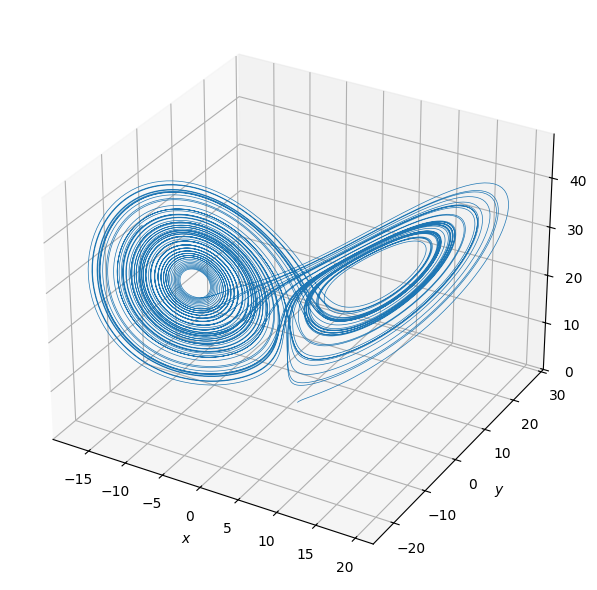
\includegraphics[width=0.6\textwidth]{Lorentz.png}
  \caption{El atractor de Lorenz.}
  \label{fig:Lorentz}
\end{figure}

Sin embargo, en dimensión dos la situación se simplifica notablemente. En este caso es posible dar una descripción completa de los posibles conjuntos $\omega$-límite para cualquier ecuación diferencial ordinaria. Este es el contenido del Teorema de Poincaré--Bendixon.

\begin{teo}[Poincaré--Bendixon]
Todo conjunto límite compacto y no vacío de un flujo en dimensión dos, definido por un campo de clase $C^1$, que no contiene puntos de equilibrio, es una órbita cerrada.
\end{teo}

Una demostración de este resultado puede encontrarse, por ejemplo, en \cite{Hirsch-Smale}.

\begin{defi}
Un {\em ciclo límite} es una órbita cerrada $\gamma$ tal que $\gamma\subset L_\omega(\xx)$ o $\gamma\subset L_\alpha(\xx)$ para algún punto $\xx\notin\gamma$.
\end{defi}

Las órbitas cerradas que rodean a un centro no son ciclos límite. Un ciclo límite es, en cambio, una órbita cerrada aislada: existe un entorno anular del ciclo que no contiene ninguna otra órbita cerrada.

El Teorema de Poincaré--Bendixon es una herramienta poderosa para demostrar la existencia de ciclos límite. En efecto, si se logra encontrar una región $D\subset\R^2$ que sea {\em positivamente invariante} para el flujo $\phi_t$ (es decir, tal que $\xx\in D$ implica $\phi_t(\xx)\in D$ para todo $t>0$) y que no contenga puntos de equilibrio, entonces el teorema garantiza la existencia de un ciclo límite contenido en $D$.

\begin{ejem}\label{ej:ciclo_limite}
Consideremos el siguiente sistema en dimensión dos:
\[
\begin{cases}
\dot x = x - y - x(x^2+y^2),\\
\dot y = x + y - y(x^2+y^2).
\end{cases}
\]
Si reescribimos este sistema en coordenadas polares obtenemos
\[
\dot r = r - r^3, \qquad \dot\theta = 1.
\]
Observamos que la solución $r=1$, $\theta=t$ corresponde a una órbita cerrada. Además, si tomamos $0<r_1<1<r_2$, se verifica que $\dot r>0$ para $r_1<r<1$ y $\dot r<0$ para $1<r<r_2$. En consecuencia, el conjunto
\[
D=\{(x,y)\colon r_1^2\le x^2+y^2\le r_2^2\}
\]
es positivamente invariante y no contiene puntos de equilibrio. Por el Teorema de Poincaré--Bendixon, este conjunto contiene un ciclo límite.
\end{ejem}

\begin{figure}[ht]
  \centering
  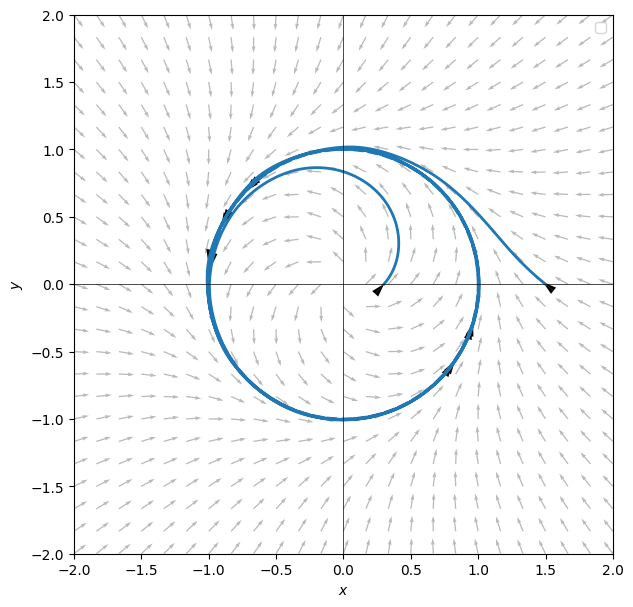
\includegraphics[width=0.6\textwidth]{ciclo_limite.png}
  \caption{Diagrama de fases para el Ejemplo~\ref{ej:ciclo_limite}.}
  \label{fig:ciclo_limite}
\end{figure}

\begin{volvemos}{el circuito}
El sistema de van der Pol \eqref{eq:vdP-sistema} es el ejemplo histórico de ciclo límite, y el Teorema de Poincaré--Bendixson es la herramienta para demostrar que existe. Sabemos que para $\lambda>0$ el origen es una fuente (Capítulo \ref{cap:HG}) y que la energía decrece cuando $|x|>1$ (Sección \ref{sec:energia-herramienta}). Para aplicar el teorema hace falta construir una región anular $D$ positivamente invariante que rodee al origen sin contenerlo: el borde interior puede ser un círculo chico (que las trayectorias cruzan hacia afuera, porque el origen es una fuente), pero el borde exterior no puede ser un círculo, porque en la franja $|x|<1$ la energía crece y las trayectorias salen de cualquier disco. La construcción correcta usa un contorno adaptado al campo y es laboriosa; puede verse en \cite{Strogatz} o \cite{Perko}. El resultado, que enunciamos sin demostración, es más general y se debe a Liénard (1928):

\begin{teo}[Liénard]\label{teo:lienard}
Consideremos la ecuación $\ddot x + f(x)\dot x + g(x) = 0$ con $f,g$ de clase $C^1$, $g$ impar con $g(x)>0$ para $x>0$, $f$ par, y tal que $G(x) = \int_0^x f(s)\,ds$ es negativa en $(0,a)$, positiva y creciente en $(a,\infty)$ y tiende a $+\infty$. Entonces la ecuación tiene una única órbita cerrada, que es un ciclo límite estable y atrae a todas las trayectorias salvo el origen.
\end{teo}

La ecuación de van der Pol es el caso $f(x) = \lambda(x^2-1)$, $g(x)=x$, con $G(x) = \lambda(x^3/3 - x)$ y $a=\sqrt3$. Queda así respondida la segunda pregunta de la Sección \ref{sec:conductor-vdP}: para todo $\lambda>0$ el circuito termina oscilando sobre una única órbita, con una amplitud y un período que no dependen del estado inicial. Para $\lambda$ chico el ciclo es casi una circunferencia de radio $2$ y el período es cercano a $2\pi$ (la oscilación natural del circuito, $2\pi\sqrt{LC}$ en las unidades originales); para $\lambda$ grande la forma de onda se vuelve muy distinta de una sinusoide (\emph{oscilaciones de relajación}) y el período crece como $\lambda$. Estas afirmaciones se exploran numéricamente en el laboratorio.
\end{volvemos}

\begin{obs}
El modelo de bacterias \eqref{bacteria2} también puede tratarse con el Teorema de Poincaré--Bendixson: para $k>k_c$ el equilibrio $(1,1)$ es una fuente, y se puede construir una región del cuadrante positivo, acotada y positivamente invariante, de la que se extrae un disco chico alrededor de $(1,1)$; el teorema garantiza entonces un ciclo límite dentro de esa región. Los detalles se proponen como ejercicio guiado. Notemos la diferencia con Lotka--Volterra \eqref{LV1}: allí las órbitas cerradas no son ciclos límite, porque ninguna es aislada, y el teorema tampoco se aplica, porque toda región anular positivamente invariante está llena de órbitas cerradas.
\end{obs}

\section{Estudio gráfico de sistemas en dimensión dos}

En esta sección presentamos algunas estrategias gráficas para determinar el diagrama de fases de sistemas de ecuaciones diferenciales ordinarias en dimensión dos, en particular de sistemas de la forma
\[
\dot N_1 = N_1 f_1(N_1,N_2), \qquad \dot N_2 = N_2 f_2(N_1,N_2).
\]

Este tipo de sistemas aparece con frecuencia en el modelado de poblaciones. Ya hemos visto ejemplos en el estudio de las ecuaciones de Lotka--Volterra (Secciones~\ref{sec:LV1} y \ref{sec:LV2}), donde $N_1$ y $N_2$ representan dos poblaciones cuyas tasas de crecimiento relativas $\dot N_i/N_i$ están dadas por las funciones $f_i(N_1,N_2)$.

La idea general del análisis geométrico es la siguiente:
\begin{enumerate}
\item Dividir el cuadrante positivo del plano $(N_1,N_2)$ en regiones delimitadas por las {\em nulclinas}
\[
\mathcal N_i=\{(N_1,N_2)\colon f_i(N_1,N_2)=0\}.
\]
\item En cada región, determinar el signo de las tasas de crecimiento y, por lo tanto, la dirección del campo vectorial.
\item Representar gráficamente estas direcciones mediante flechas.
\end{enumerate}

Veamos cómo aplicar esta estrategia en un ejemplo concreto.

\begin{ejem}[Competencia de especies]
Supongamos que dos especies compiten por un mismo recurso. Su evolución puede modelarse mediante el sistema
\[
\begin{cases}
\dot N_1 = r_1 N_1\left(1-\frac{N_1}{K_1}\right) - \lambda_1 N_1 N_2,\\
\dot N_2 = r_2 N_2\left(1-\frac{N_2}{K_2}\right) - \lambda_2 N_1 N_2.
\end{cases}
\]
Cada población $N_i$ presenta un crecimiento logístico con tasa intrínseca $r_i$ y capacidad de carga $K_i$, mientras que la presencia de la otra especie reduce su tasa de crecimiento. Todas las constantes se asumen positivas.

Procedemos a adimensionalizar el sistema introduciendo las variables
\[
\tau=\sqrt{r_1r_2}\,t,\quad \rho=\sqrt{\frac{r_1}{r_2}},\quad n_i=\frac{N_i}{K_i},\ i=1,2,
\]
y los parámetros
\[
\alpha_1=\frac{\lambda_1K_2}{\sqrt{r_1r_2}},\qquad \alpha_2=\frac{\lambda_2K_1}{\sqrt{r_1r_2}}.
\]
\end{ejem}

El sistema se reduce entonces a
\[
\begin{cases}
n_1'=\rho n_1(1-n_1)-\alpha_1 n_1 n_2,\\
n_2'=\frac{1}{\rho}n_2(1-n_2)-\alpha_2 n_1 n_2,
\end{cases}
\]
donde el número de parámetros se ha reducido de seis a tres.

Las nulclinas están dadas por
\[
\mathcal N_1=\{\rho(1-n_1)-\alpha_1 n_2=0\}, \qquad
\mathcal N_2=\left\{\frac{1}{\rho}(1-n_2)-\alpha_2 n_1=0\right\}.
\]
La coexistencia de ambas especies es posible si y sólo si $\mathcal N_1\cap\mathcal N_2\neq\emptyset$.

Esta intersección puede caracterizarse en términos de las cantidades
\[
a_1=\frac{\rho}{\alpha_1}, \qquad a_2=\frac{1}{\rho\alpha_2}.
\]
Es fácil ver que $\mathcal N_1\cap\mathcal N_2\neq\emptyset$ si y sólo si se verifica una de las condiciones
\[
a_1>1 \text{ y } a_2>1 \qquad \text{o} \qquad a_1<1 \text{ y } a_2<1.
\]

Ver Figura~\ref{fig:nulclinas}.

\begin{figure}[ht]
  \centering
  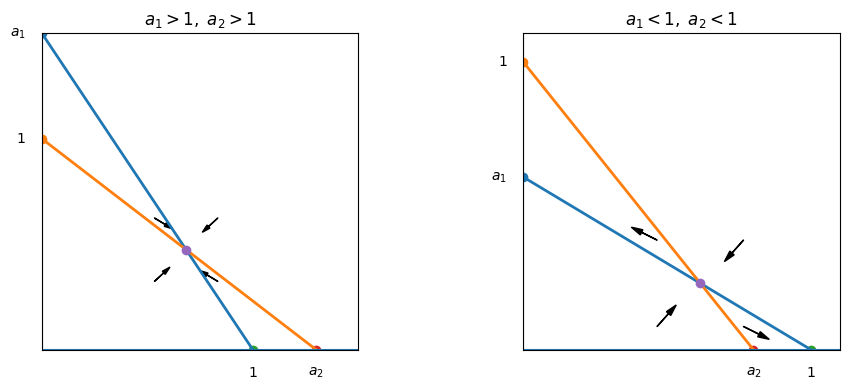
\includegraphics[width=0.6\textwidth]{nulclinas.png}
  \caption{Gráfico de las nulclinas en los casos $a_i>1$ (izquierda) y $a_i<1$ (derecha), $i=1,2$.}
  \label{fig:nulclinas}
\end{figure}

El análisis del campo vectorial muestra que el equilibrio de coexistencia es asintóticamente estable cuando $a_1,a_2>1$, mientras que resulta ser un punto silla cuando $a_1,a_2<1$.

En los casos $a_1<1<a_2$ y $a_2<1<a_1$ las nulclinas no se intersectan, por lo que la coexistencia no es posible. Queda como ejercicio para el lector realizar el diagrama de fases en estas situaciones.


\chapter{Bifurcaciones}\label{cap:bifurcaciones}

En general uno espera que las propiedades cualitativas de un modelo no cambien significativamente cuando el mismo es modificado levemente. Es decir, un modelo debe ser {\em robusto} para pequeñas perturbaciones. Esta propiedad en un modelo se la denomina {\em estabilidad estructural}.

Por otro lado, si uno continúa perturbando el modelo, ocurre que a partir de un cierto {\em umbral} de perturbaciones se observa que el mismo presenta un cambio en su dinámica (por ejemplo, aparecen nuevos puntos estacionarios, puntos estacionarios modifican su dinámica, etc). Ese cambio repentino en la dinámica de un sistema se lo denomina una {\em bifurcación}.

En este capítulo intentaremos dar precisiones sobre estos conceptos y dar una breve introducción a los distintos tipos de bifurcaciones que pueden ocurrir.

\section{Estabilidad estructural}

Para definir este concepto, primero tenemos que entender lo que significa realizar una perturbación de un modelo. Una EDO viene determinada por un campo vectorial $F\colon\R^n\to\R^n$. Para que la EDO esté bien definida, precisamos que el campo sea de clase $C^1$.

Perturbar levemente el campo $F$ significa modificar el campo $F$ manteniéndolo {\em cerca} del mismo. Pero para eso tenemos que definir qué significa estar cerca.

La forma estándar de realizar eso es a través de una norma $\|\cdot\|$ y decir que $F$ y $G$ están cerca si $\|F-G\|$ es chico. Pero ¿qué norma conviene utilizar?

La primera opción es utilizar la norma $C^0$, es decir
$$
\|F\|_0 = \sup_{\xx\in U} |F(\xx)|
$$
donde $|\cdot|$ es la norma euclidea en $\R^n$ y $U$ es un abierto de $\R^n$ con clausura compacta.

\begin{figure}[ht]
  \centering
  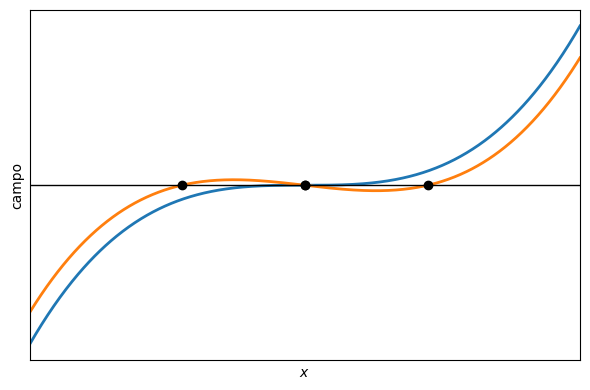
\includegraphics[width=0.6\textwidth]{c0-cerca.png}
  \caption{Dos campos $C^0$ cerca pero cuyos flujos presentan un diferente comportamiento dinámico.}
  \label{fig:c0-cerca}
\end{figure}

Como se ve en la Figura \ref{fig:c0-cerca}, dos campos cercanos en la norma $C^0$ no tienen necesariamente el mismo número de puntos de equilibrio hiperbólicos. Necesitamos entonces una noción de proximidad más fuerte que requiera que tanto la función como sus derivadas sean próximas. Para eso se define la norma $C^1$ como
$$
\|F\|_1 = \sup_{\xx\in U} \Big(|F(\xx)| + \|DF(\xx)\|\Big),
$$
donde $\|A\|$ es una norma en el espacio de matrices $\R^{n\times n}$. Por ejemplo
$$
\|A\| = \left(\sum_{i,j=1}^n a_{ij}^2\right)^\frac12
$$

De manera análoga se pueden seguir definiendo las normas $\|\cdot\|_k$ que miden la proximidad de las funciones y sus derivadas hasta orden $k$.

Llamaremos $\F(U)$ al espacio de todos los campos vectoriales $F\colon U\to\R^n$ de clase $C^1$ con norma $\|\cdot\|_1$. Definimos entonces el $\ve-$entorno de $F\in\F(U)$ como
$$
N_\ve(F) = \{G\in\F(U)\colon \|F-G\|_1<\ve\}.
$$
Un campo $G\in N_\ve(F)$ se dice que está $\ve-C^1-$cerca de $F$ o que es una $\ve-C^1-$perturba-ción de $F$.

\begin{teo}\label{teo:est.est}
Sea $\xx^*$ un punto fijo hiperbólico del flujo $\phi_t$ generado por el campo $F\in \F(U)$. Entonces existe un entorno $V$ de $\xx^*$ y $\ve>0$ tal que si $G\in N_\ve(F)$, entonces $G$ genera un flujo $\psi_t$ que tiene un único punto fijo hiperbólico $\yy^*\in V$. Más aún, las matrices diferenciales $DF(\xx^*)$ y $DG(\yy^*)$ tienen el mismo número de autovalores con parte real positiva y negativa. 
\end{teo}

\begin{proof}
Para una demostración de este resultado, se puede consultar a \cite{Hirsch-Smale-Devaney, Perko}. Hagamos un boceto de la demostración en el caso paramétrico. Es decir, en el caso en que $G(\xx) = F(\xx, \mu)$ donde $\mu\in\R^r$ es un conjunto de parámetros.

Supongamos que para un cierto valor de los parámetros $\mu^*$ tenemos un punto fijo hiperbólico $\xx^*$. Entonces, si los autovalores de $DF(\xx^*,\mu^*)$ tienen parte real no nula, podemos aplicar el Teorema de la Función Implícita y concluir que existe una única función $\xx(\mu)$ definida para $\mu$ cerca a $\mu^*$ tal que
$$
F(\xx(\mu),\mu)=0 \qquad \text{y}\qquad \xx(\mu^*)=\xx^*.
$$
Por otro lado, como los autovalores de $DF(\xx(\mu),\mu)$ son continuos con respecto a $\mu$, para $\mu$ cerca de $\mu^*$ todos los autovalores van a tener aún parte real distinta de cero. Luego los puntos de equilibrio cercanos a $(\xx^*,\mu^*)$ también resultan hiperbólicos y con la misma estabilidad que $(\xx^*,\mu^*)$.
\end{proof}

Cuando estamos en presencia de puntos fijos no hiperbólicos el Teorema \ref{teo:est.est} ya no es cierto y hemos visto varios ejemplos de esa situación en estas notas.

Por ejemplo, el campo $F(x, y) = (y, -\omega^2\sin x)$ representa el péndulo simple. El origen es un equilibrio no hiperbólico. El péndulo amortiguado viene dado por el campo $G(x, y) = (y, -\omega^2\sin x - 2a y)$. Si $a$ es pequeño, $G$ es una $\ve-C^1-$perturbación de $F$, sin embargo la dinámica de $G$ es diferente a la de $F$ dado que el origen es un equilibrio hiperbólico asintóticamente estable.

\section{Bifurcaciones locales}

En la Sección \ref{sec:ciclo_limite} estudiamos el siguiente sistema
$$
\begin{cases}
h' = h\left(1-\frac{h}{k}\right) - \frac{\alpha_h ph}{\beta + h}\\
p' = \frac{\alpha_p ph}{\beta + h} - \gamma p,
\end{cases}
$$
donde 
$$
\alpha_h = \left(1-\frac{1}{k}\right) (\beta+1)\quad \text{y}\quad \alpha_p = \gamma(\beta+1).
$$
Este sistema exhibe dos comportamientos cualitativos bien diferentes. Para $k<\beta+2$ el punto de equilibrio $(1,1)$ es asintóticamente estable, pero para $k>\beta+2$ el punto $(1,1)$ es inestable y el $\omega-$límite es un ciclo límite. El cambio de comportamiento ocurre para $k=\beta+2$, esto es cuando el punto $(1,1)$ no es hiperbólico. Este cambio de comportamiento en un sistema ante una variación leve de sus parámetros es lo que llamamos una {\em bifurcación}.

Hemos visto varios ejemplos de este fenómeno a lo largo de las notas (ver, por ejemplo, el oscilador de van der Pol, Sección \ref{sec:conductor-vdP}).

Supongamos que tenemos una familia de campos indexados por un vector de parámetros $F(\xx, \mu)$ donde $\mu\in\R^r$. Supongamos que para un cierto valor de los parámetros $\mu^*$, tenemos un equilibrio $\xx^*$ para el flujo generado (i.e. $F(\xx^*, \mu^*)=0$). La pregunta que buscamos responder es: ¿Se preserva la estabilidad del equilibrio $\xx^*$ cuando variamos los parámetros $\mu$?

Si el equilibrio es hiperbólico, entonces por el Teorema \ref{teo:est.est} sigue que el flujo generado por $F(\cdot,\mu)$ es localmente estructuralmente estable en $(\xx^*,\mu^*)$. Como consecuencia, si $\mu$ es cercano a $\mu^*$ vamos a tener un único equilibrio $\xx(\mu)$ cercano a $\xx^*$ y la estabilidad de $\xx(\mu)$ es la misma que la de $\xx^*$.

Por otro lado, si el equilibrio $(\xx^*,\mu^*)$ no es hiperbólico, el campo $F(\xx, \mu)$ no es estructuralmente estable en $(\xx^*,\mu^*)$. En este caso para valores de $\mu$ cercanos a $\mu^*$ puede ocurrir un comportamiento dinámico completamente diferente.

En este capítulo vamos a investigar las bifurcaciones más simples que pueden aparecer en puntos de equilibrio no hiperbólicos en sistemas en dimensión 1 y 2.

\section{Bifurcaciones para campos vectoriales unidimensionales}

En un sistema en dimensión uno, un punto de equilibrio no hiperbólico está asociado a un cero de la derivada del campo en el equilibrio. 

En esta sección vamos a describir los tipos más importantes de bifurcaciones para ecuaciones del tipo
$$
\dot x = f(x,\mu)\qquad (x\in\R, \mu\in\R).
$$
Sin pérdida de generalidad, podemos suponer que $(x^*,\mu^*)=(0,0)$, luego
$$
f(0,0)=0\qquad \text{y}\qquad \frac{\partial f}{\partial x}(0,0)=0.
$$

\subsection*{Bifurcación silla-nodo}

Consideremos la ecuación
\begin{equation}\label{eq:saddle-node}
\dot x = \mu - x^2.
\end{equation}
Para $\mu=0$, $x^*=0$ es el único punto de equilibrio y no es hiperbólico dado que $f_x(0,0)=0$, luego el sistema no es estructuralmente estable. Para $\mu<0$ no hay equilibrios mientras que para $\mu>0$ hay dos equilibrios $x^*=\pm\sqrt{\mu}$. Como $f_x(\pm\sqrt{\mu}, \mu) = \mp2\sqrt{\mu}$, $\sqrt{\mu}$ es asintóticamente estable y $-\sqrt{\mu}$ es inestable. Los diagramas de fase respectivos los pueden ver en la Figura \ref{fig:saddle-node}.

\begin{figure}[ht]
  \centering
  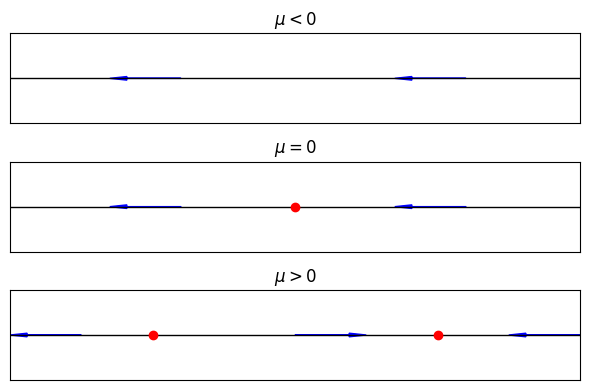
\includegraphics[width=0.6\textwidth]{saddle-node.png}
  \caption{Diagramas de fase de \eqref{eq:saddle-node} para distintos valores de $\mu$.}
  \label{fig:saddle-node}
\end{figure}

Toda la información de la bifurcación se suele resumir en un {\em diagrama de bifurcación}. Ver Figura \ref{fig:diagrama-saddle-node}. Este diagrama grafica en el plano $(\mu, x)$ a la curva de equilibrios $\mu-x^2=0$, se grafica con línea llena cuando es estable y con línea puntuada cuando es inestable. Para cada valor de $\mu$ fijo, la línea vertical refleja el diagrama de fases de la ecuación \eqref{eq:saddle-node} para ese valor de $\mu$. Comparar con la Figura \ref{fig:saddle-node}.
\begin{figure}[ht]
  \centering
  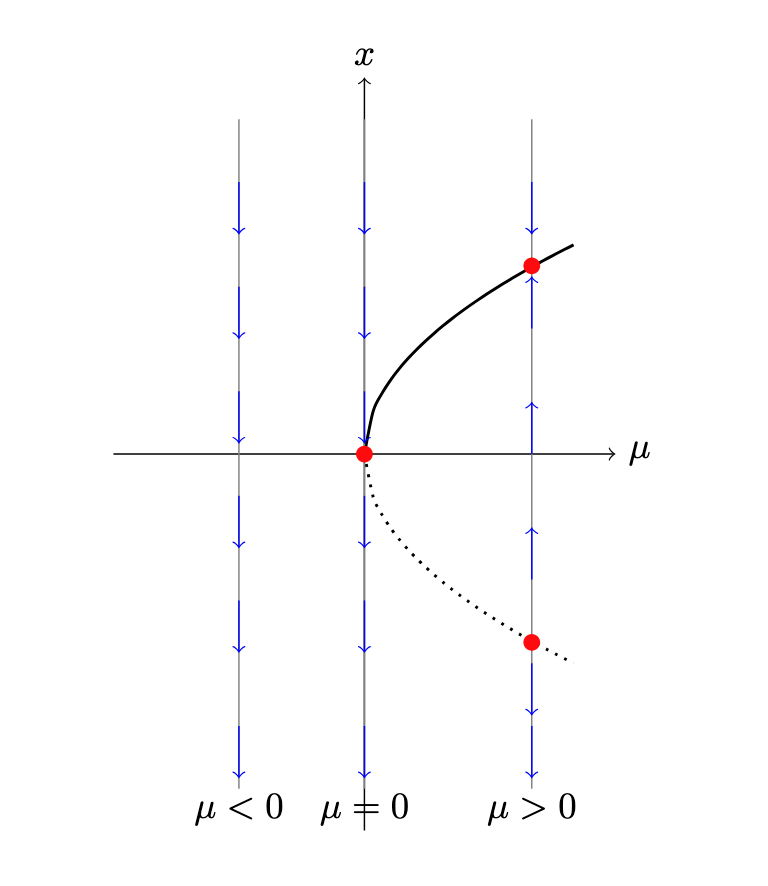
\includegraphics[width=0.6\textwidth]{diagrama-saddle-node.png}
  \caption{Diagrama de bifurcación para \eqref{eq:saddle-node}.}
  \label{fig:diagrama-saddle-node}
\end{figure}

\subsection*{Bifurcación transcrítica}

Consideremos ahora la ecuación
\begin{equation}\label{eq:transcritica}
\dot x = \mu x - x^2.
\end{equation}
Para $\mu=0$, el único equilibrio es $x^*=0$. Este punto no es hiperbólico, dado que $f_x(0,0)=0$, luego el campo $f(x, 0)$ no es estructuralmente estable y $\mu=0$ es un punto de bifurcación. Para valores $\mu\neq 0$, tenemos dos equilibrios, $\mu$ y $0$. En la bifurcación, estos dos equilibrios intercambian su estabilidad. Ver la Figura \ref{fig:transcritica}. Este tipo de bifurcación se llama {\em transcrítica}.
\begin{figure}[ht]
  \centering
  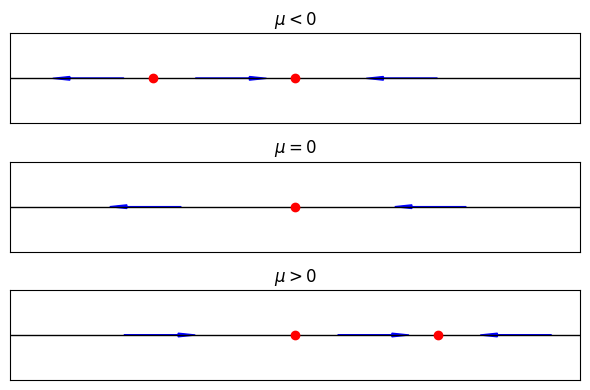
\includegraphics[width=0.6\textwidth]{transcritica.png}
  \caption{Diagramas de fases para \eqref{eq:transcritica}.}
  \label{fig:transcritica}
\end{figure}

El diagrama de bifurcación para \eqref{eq:transcritica} está en la Figura \ref{fig:diagrama-transcritica}.
\begin{figure}[ht]
  \centering
  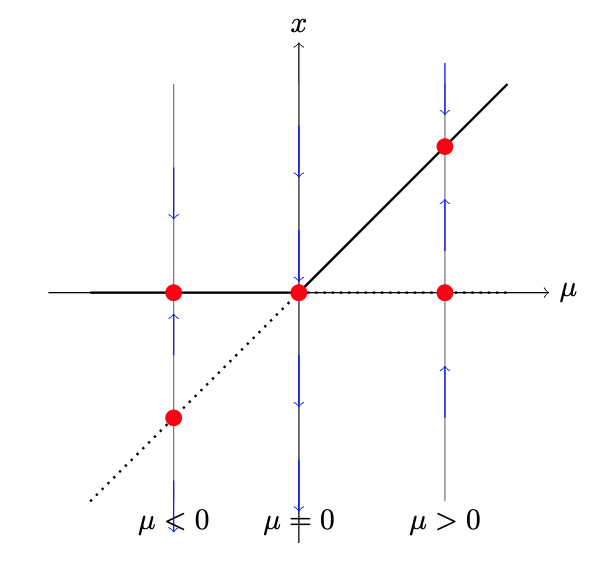
\includegraphics[width=0.6\textwidth]{diagrama-transcritica.png}
  \caption{Diagrama de bifurcación para \eqref{eq:transcritica}.}
  \label{fig:diagrama-transcritica}
\end{figure}

\subsection*{Bifurcación de horquilla (pitchfork)}

Consideremos la ecuación
\begin{equation}\label{eq:pitchfork}
\dot x = \mu x - x^3.
\end{equation}
Al igual que en \eqref{eq:transcritica}, para $\mu=0$ el único equilibrio es $x^*=0$ que no es hiperbólico y el campo $f(x, 0)$ no es estructuralmente estable. Luego $\mu=0$ es un punto de bifurcación. Observemos que si $\mu\le 0$ el único punto de equilibrio sigue siendo $x^*=0$, pero para $\mu>0$ tenemos tres equilibrios: $0$, que es inestable, y $\pm\sqrt{\mu}$ que son asintóticamente estables. Los diagramas de fases para \eqref{eq:pitchfork} se pueden ver en la Figura \ref{fig:pitchfork}.
\begin{figure}[ht]
  \centering
  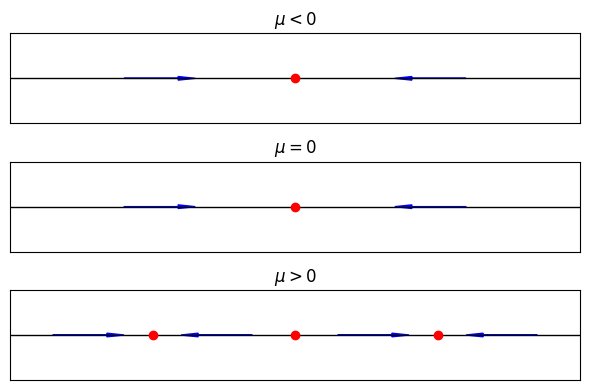
\includegraphics[width=0.6\textwidth]{pitchfork.png}
  \caption{Diagramas de fases para \eqref{eq:pitchfork}.}
  \label{fig:pitchfork}
\end{figure}
El diagrama de bifurcación para \eqref{eq:pitchfork} está en la Figura \ref{fig:diagrama-pitchfork}.
\begin{figure}[ht]
  \centering
  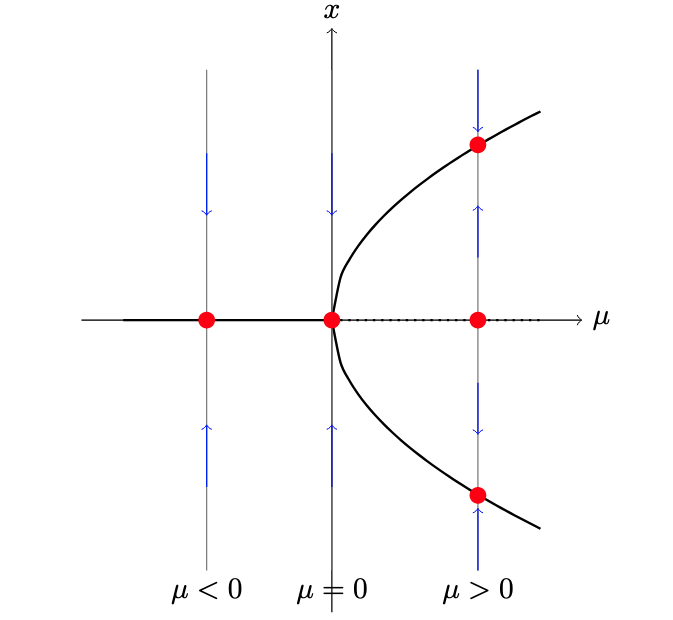
\includegraphics[width=0.6\textwidth]{diagrama-pitchfork.png}
  \caption{Diagrama de bifurcación para \eqref{eq:pitchfork}.}
  \label{fig:diagrama-pitchfork}
\end{figure}

\subsection*{Campos generales}

Los casos vistos en \eqref{eq:saddle-node}, \eqref{eq:transcritica} y \eqref{eq:pitchfork} son los casos canónicos de sistemas más generales.

Supongamos que tenemos el sistema
\begin{equation}\label{eq:general}
\dot x = f(x, \mu)
\end{equation}
y supongamos que para $\mu^*$ tenemos que $x^*$ es un punto de equilibrio no hiperbólico. Es decir
\begin{equation}\label{no-hiper}
f(x^*, \mu^*)=0\quad \text{y}\quad f_x(x^*,\mu^*)=0.
\end{equation}
Sin pérdida de generalidad y para simplificar la exposición, podemos suponer que $(x^*, \mu^*)=(0,0)$. Como $0$ es un equilibrio no hiperbólico, tenemos que $\mu=0$ es un punto de bifurcación para \eqref{eq:general}. Como el análisis de bifurcación es un análisis local cerca del punto $(0,0)$ hacemos una expansión de Taylor para $f$ para realizar el análisis.

\subsubsection*{Silla-nodo}
Por Taylor,
$$
f(x,\mu) = \underbrace{f(0,0)}_{0} + \underbrace{f_x(0,0) x}_{0} + f_\mu(0,0)\mu + \frac12 f_{xx}(0,0) x^2 + \text{términos de mayor orden}.
$$
Luego, si asumimos que $f_\mu(0,0)=a\neq0$ y $f_{xx}(0,0)=-2b\neq 0$, tenemos que
$$
f(x, \mu) \sim a\mu - bx^2.
$$
Observemos la similitud con \eqref{eq:saddle-node}, lo que hace suponer que estamos en presencia de una bifurcación de tipo silla-nodo.

Como $f_\mu(0,0)\neq 0$ podemos usar el Teorema de la función implícita (TFI) y obtenemos que existe un único despeje de la ecuación
$$
f(x,\mu)=0.
$$
Es decir, existe una función $\mu=\mu(x)$ tal que $\mu(0)=0$ y $f(x,\mu(x))=0$ para todo $x\sim 0$. Más aún, se tiene que
$$
\frac{d\mu}{dx}(0) = -\frac{f_x(0,0)}{f_\mu(0,0)} = 0.
$$
Por otro lado, derivando respecto a $x$ dos veces la expresión $f(x,\mu(x))=0$ y evaluando en $x=0$ llegamos a
$$
f_{xx}(0,0) + 2f_{x\mu}(0,0)\underbrace{\frac{d\mu}{dx}(0)}_{0} + f_{\mu\mu}(0,0) \underbrace{\left(\frac{d\mu}{dx}(0)\right)^2}_{0} + f_\mu(0,0)\frac{d^2\mu}{dx^2}(0) = 0,
$$
de donde
$$
\frac{d^2\mu}{dx^2}(0) = -\frac{f_{xx}(0,0)}{f_\mu(0,0)} = \frac{2b}{a} \neq 0.
$$
Es decir, la curva $x\mapsto \mu(x)$ tiene la expresión
$$
\mu(x) = \underbrace{\mu(0)}_{0} + \underbrace{\frac{d\mu}{dx}(0)}_{0} x + \frac12 \underbrace{\frac{d^2\mu}{dx^2}(0)}_{\frac{2b}{a}} x^2 +\cdots = \frac{b}{a}x^2 + \cdots
$$
En síntesis, el sistema \eqref{eq:general} exhibe una única curva de equilibrios cerca de $(0,0)$, esta curva se encuentra a un lado de la recta $\mu=0$ en el plano $(\mu, x)$ y es tangente a la recta $\mu=0$ en el punto $(0,0)$. Su diagrama de bifurcación entonces coincide con el de una silla-nodo (Figura \ref{fig:diagrama-saddle-node}).

\subsubsection*{Transcrítica}

Supongamos ahora que, adicionalmente a \eqref{no-hiper} (con lo que $(0,0)$ es un equilibrio no hiperbólico), tenemos que, a diferencia con el caso anterior,
$$
f_{\mu}(0,0)=0.
$$
Luego, en la expansión de Taylor de $f$ debemos incorporar el primer término no nulo que contenga a $\mu$, es decir
\begin{equation}\label{Taylor-transcritica}
f(x, \mu) = f_{x\mu}(0,0)\mu x + \frac12 f_{xx}(0,0)x^2 + \cdots
\end{equation}
Asumamos que $f_{x\mu}(0,0)=a\neq 0$ y que $f_{xx}(0,0)=-2b\neq 0$ con lo cual
$$
f(x,\mu)\sim a\mu x - bx^2.
$$
Observemos la similitud con \eqref{eq:transcritica}. En este caso, como $f_\mu(0,0)=0$ no podemos usar el TFI para despejar $\mu$ de $f(x,\mu)=0$ (y eso es deseable dado que esperamos la existencia de 2 curvas de equilibrios cercanos a $(0,0)$, c.f. Figura \ref{fig:diagrama-transcritica}). Sin embargo si dividiendo por $x$ en \eqref{Taylor-transcritica} obtenemos
$$
g(x,\mu) = \frac{f(x, \mu)}{x} = f_{x\mu}(0,0)\mu + \frac12 f_{xx}(0,0)x + \cdots.
$$
Tenemos entonces que $f(x,\mu)= xg(x,\mu)$ y usando las reglas de derivación, junto con \eqref{no-hiper} obtenemos:
\begin{equation}\label{deriv.g}
g(0,0) = f_x(0,0) = 0, \quad g_x(0,0) = f_{xx}(0,0)\neq 0\quad \text{y}\quad g_{\mu}(0,0) = f_{x\mu}(0,0)\neq 0.
\end{equation}
Observemos entonces que podemos usar el TFI para despejar $\mu$ de la ecuación $g(x,\mu)=0$ obteniendo $\mu=\mu(x)$ tal que $\mu(0)=0$ y $g(x,\mu(x))=0$ para todo $x\sim 0$.

Derivando la expresión $g(x,\mu(x))=0$ se obtiene
$$
\frac{d\mu}{dx}(0) = -\frac{g_x(0,0)}{g_\mu(0,0)} = -\frac{f_{xx}(0,0)}{f_{x\mu}(0,0)} = \frac{2b}{a}\neq 0.
$$

En resumen, el sistema \eqref{eq:general} presenta una bifurcación transcrítica dado que en un entorno del $(0,0)$ obtenemos dos curvas de equilibrios. Una $(0,\mu)$ y otra $(x,\mu(x))$ con $\mu(x)\sim \frac{2b}{a}x$. Ver Figura \ref{fig:diagrama-transcritica}.

\subsubsection*{Horquilla}

Vamos a argumentar de manera similar al caso anterior. Asumamos que ahora, además de
$$
f(0,0)=0,\ f_x(0,0)=0,\ f_\mu(0,0)=0,
$$
se tiene que $f_{xx}(0,0)=0$. Luego, el desarrollo de Taylor de $f$ en un entorno del $(0,0)$ es
$$
f(x, \mu) = f_{x\mu}(0,0)\mu x +  \frac{1}{6}f_{xxx}(0,0) x^3 + \cdots
$$
Observemos que en una bifurcación tipo horquilla, es esperable que cerca del $(0,0)$ la rama de equilibrios $(x,\mu)$ verifique la relación $\mu\sim x^2$. Por ende los términos de 2do y 3er orden en la expansión de Taylor restantes van a resultar de mayor orden y por eso se descartan. En efecto:
$$
\mu^2 \sim x^4,\quad x\mu^2\sim x^5,\quad x^2\mu\sim x^4,
$$
mientras que
$$
\mu x \sim x^3.
$$

Ahora, al igual que en el caso de la bifurcación transcrítica, escribimos
$$
f(x,\mu) = x g(x, \mu)
$$
entonces, vale \eqref{deriv.g}, con la diferencia que ahora $g_x(0,0) = 0$, y además se tiene
$$
g_{xx}(0,0) = f_{xxx}(0,0). 
$$
Argumentando como en el caso anterior, tenemos la existencia de una única curva $x\mapsto\mu(x)$ tal que
$$
g(x, \mu(x))=0,\quad \mu(0)=0
$$
y diferenciando, obtenemos
\begin{align*}
&\frac{d\mu}{dx}(0) = -\frac{g_x(0,0)}{g_\mu(0,0)} = -\frac{f_{xx}(0,0)}{f_{x\mu}(0,0)} = 0\\
&\frac{d^2\mu}{dx^2}(0) = -\frac{g_{xx}(0,0)}{g_\mu(0,0)} = -\frac{f_{xxx}(0,0)}{f_{x\mu}(0,0)} \neq 0.
\end{align*}
En consecuencia tenemos dos curvas de equilibrios, una  que es aproximadamente $(0,\mu)$ y la otra $(x,\mu(x))$ con $\mu(x) \sim cx^2$. Ver Figura \ref{fig:diagrama-pitchfork}.

\subsection{Resumen}

Supongamos que tenemos un sistema $\dot x = f(x, \mu)$ tal que $f(0,0)=0$ y queremos ver si $\mu=0$ es un punto de bifurcación y, en ese caso, clasificar el tipo de bifurcación. Entonces se procede de la siguiente forma:
\begin{itemize}
\item Si $f_x(0,0)\neq 0$ entonces el equilibrio es hiperbólico y hay estabilidad estructural.

\item Si $f_x(0,0)=0$ entonces el equilibrio no es hiperbólico y estamos frente a una posible bifurcación.
\end{itemize}

Supongamos entonces que $f_x(0,0)=0$, luego calculamos $f_\mu(0,0)$ y se nos presenta la siguiente alternativa:
\begin{enumerate}
\item Si $f_\mu(0,0)\neq 0$, entonces sale una única curva de puntos críticos $x\mapsto\mu(x)$ tal que $f(x,\mu(x))=0$. Posible silla-nodo.

Calculamos entonces $f_{xx}(0,0)$.
\begin{enumerate}
\item Si $f_{xx}(0,0)\neq 0$ tenemos una bifurcación silla-nodo (Figura \ref{fig:diagrama-saddle-node}).

\item Si $f_{xx}(0,0)=0$ no tenemos clasificación disponible.
\end{enumerate}

\item Si $f_\mu(0,0)=0$, entonces existe más de una curva de puntos críticos. Posible bifurcación transcrítica o tipo horquilla. 

Calculamos entonces $f_{x\mu}(0,0)$. Si $f_{x\mu}(0,0)=0$ no tenemos clasificación disponible, pero si $f_{x\mu}(0,0)\neq 0$ entonces calculamos $f_{xx}(0,0)$ y
\begin{enumerate}
\item si $f_{xx}(0,0)\neq 0$ es una bifurcación transcrítica (Figura \ref{fig:diagrama-transcritica}).
\item Si $f_{xx}(0,0)=0$ es una bifurcación tipo horquilla (Figura \ref{fig:diagrama-pitchfork}).
\end{enumerate}
\end{enumerate}

\section{Bifurcaciones en dimensión 2}
Observemos que si la ecuación diferencial unidimensional $\dot x = f(x,\mu)$ presenta una bifurcación de alguno de los tipos vistos previamente, entonces el sistema bi-dimensional
$$
\begin{cases}
\dot x_1 = f(x_1,\mu)\\
\dot x_2 = -x_2
\end{cases}
$$
va a exhibir el mismo tipo de bifurcación. 

Veamos un ejemplo interesante.

\begin{ejem}
Consideremos el sistema
\begin{equation}\label{eq:bif1}
\begin{cases}
\dot x = -a x + y\\
\dot y = \frac{x^2}{1+x^2} - by
\end{cases}
\end{equation}
que es un modelo para un sistema de control genético, donde $x$ e $y$ son proporcionales a las concentraciones de proteína y RNA mensajero respectivamente. Los parámetros $a$ y $b$ son positivos. 

Nos interesa la dinámica en el primer cuadrante $x, y>0$. Los puntos estacionarios del sistema van a ser las intersecciones de las nulclinas
$$
-ax+y=0\qquad \text{y}\qquad \frac{x^2}{1+x^2} - by=0.
$$
Observemos que el $(0,0)$ siempre es un equilibrio del sistema así que buscamos los equilibrios no triviales. Es sencillo ver que si $2ab<1$ entonces hay dos puntos de equilibrio, si $2ab=1$ hay un sólo equilibrio y si $2ab>1$ no hay más equilibrios. Ver Figura \ref{fig:nulclinas-bif}
\end{ejem}
\begin{figure}[ht]
  \centering
  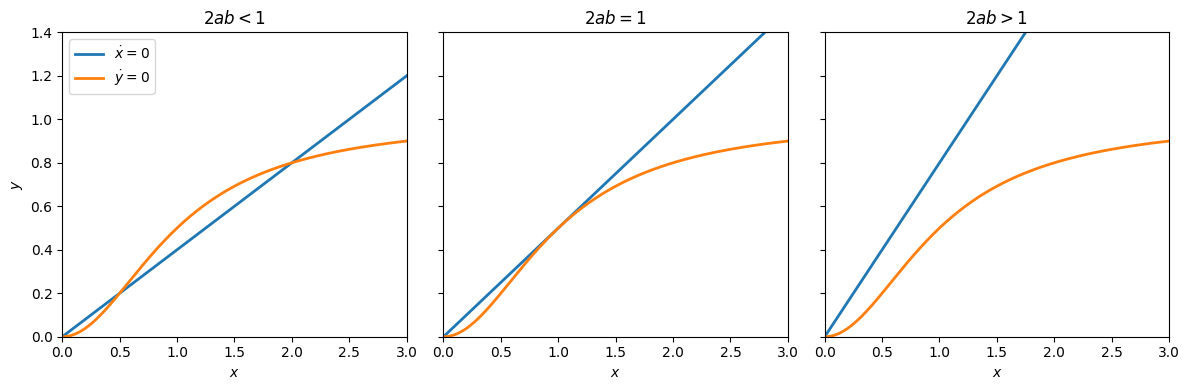
\includegraphics[width=0.8\textwidth]{nulclinas-bif.png}
  \caption{Gráfico de las nulclinas para el sistema \eqref{eq:bif1}.}
  \label{fig:nulclinas-bif}
\end{figure}

Fijemos $b>0$ y definamos $a_c=\frac{1}{2b}$. Calculemos la matriz diferencial del campo $F(x,y) = (-ax+y, \frac{x^2}{1+x^2} - by)^t$:
$$
DF(x, y) = \begin{bmatrix}
-a & 1\\
\frac{2x}{(1+x^2)^2} & -b
\end{bmatrix}
$$
Observemos que $\tau = \tr DF(x, y) = -(a+b)<0$. Luego, por el Teorema de Hartman-Grobman y el Teorema \ref{teo.lineal}, los equilibrios o bien son sillas, o bien son asintóticamente estables (sumideros).

Calculemos el determinante:
$$
\Delta = \det DF(x, y) = ab-\frac{2x}{(1+x^2)^2}.
$$

En el equilibrio trivial, $(0,0)$, tenemos que $\Delta = ab>0$ por lo que, por el Teorema \ref{teo.lineal}, resulta asintóticamente estable y si calculamos
$$
\tau^2 - 4\Delta = (a+b)^2-4ab = (a-b)^2>0, \quad \text{si } a\neq b.
$$
Nuevamente, por el Teorema \ref{teo.lineal} el origen es un nodo estable.

Si $a>a_c$ el origen es el único equilibrio. Pero si $a\le a_c$ y $(x^*, y^*)$ es un equilibrio no trivial, tenemos que $x^* = ab(1+(x^*)^2)$. Luego, tenemos
$$
\Delta = ab-\frac{2x^*}{(1+(x^*)^2)^2} = ab\left(1-\frac{2}{1+(x^*)^2}\right) = ab\left(\frac{(x^*)^2 - 1}{1+(x^*)^2}\right).
$$

Consideremos primero el caso $a<a_c$. En la Figura \ref{fig:ej-bif1} se tiene un gráfico de las nulclinas, los equilibrios y el campo vectorial.
\begin{figure}[ht]
  \centering
  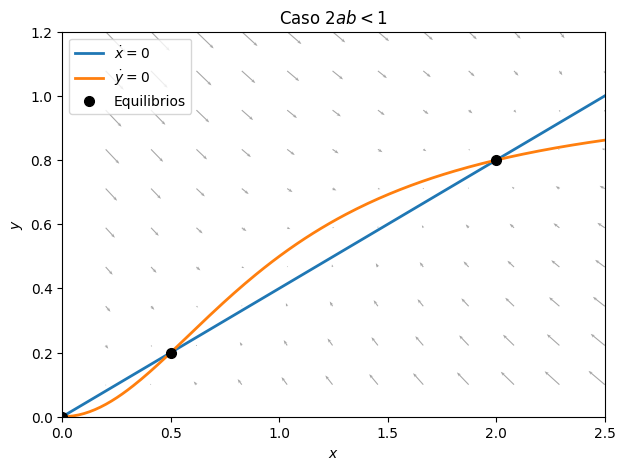
\includegraphics[width=0.6\textwidth]{ej-bif1.png}
  \caption{Gráfico de las nulclinas, equilibrios y campo vectorial en el caso $a<a_c$.}
  \label{fig:ej-bif1}
\end{figure}
En esta situación ($a<a_c$) los dos equilibrios no triviales $(x_1^*, y_1^*)$ y $(x_2^*, y_2^*)$ verifican que $x_1^*<1<x_2^*$ con lo que 
$$
\Delta_1 = \det DF(x_1^*, y_1^*) <0 \quad \text{y}\quad \Delta_2 = \det DF(x_2^*, y_2^*) >0.
$$
Luego $(x_1^*, y_1^*)$ es una silla y como $\Delta_2<ab$, tenemos que $\tau^2-4\Delta_2>(a-b)^2>0$ con lo que $(x_2^*, y_2^*)$ es un nodo estable. El diagrama de fases para este caso está en la Figura \ref{fig:ej-bif1-fases}
\begin{figure}[ht]
  \centering
  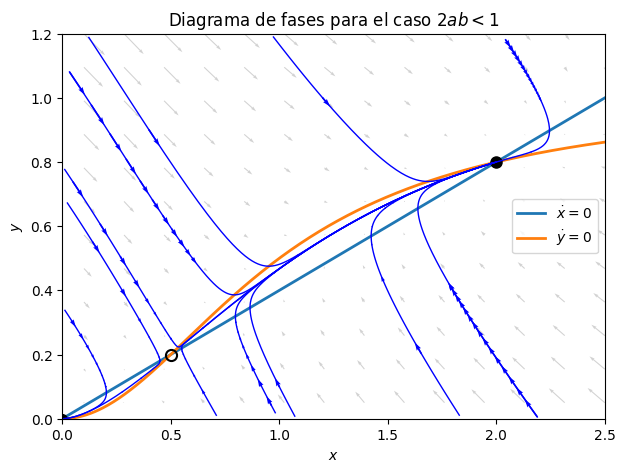
\includegraphics[width=0.6\textwidth]{ej-bif1-fases.png}
  \caption{Diagrama de fases en el caso $a<a_c$.}
  \label{fig:ej-bif1-fases}
\end{figure}

Observemos que al pasar $a$ por $a_c$ tenemos que para $a=a_c$ existe un único equilibrio no trivial que no es hiperbólico. Para $a<a_c$ se tienen dos equilibrios, uno es una silla y otro es un nodo y para $a>a_c$ no tenemos equilibrios no triviales. Es decir, estamos en presencia de una bifurcación de tipo silla-nodo.

En la Figura \ref{fig:diagrama-ej-bif1} se grafica la coordenada $x$ de los equilibrios no triviales como función del parámetro $a$. Comparar con el diagrama de bifurcación silla-nodo de la Figura \ref{fig:diagrama-saddle-node}.
\begin{figure}[ht]
  \centering
  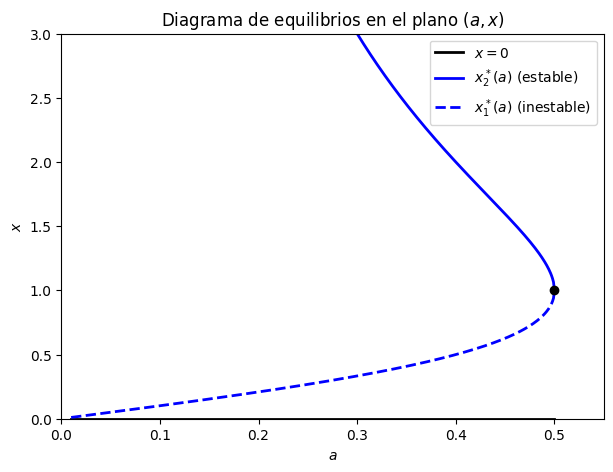
\includegraphics[width=0.6\textwidth]{diagrama-ej-bif1.png}
  \caption{Diagrama de bifurcación para \eqref{eq:bif1}. Se grafica la coordenada $x$ de los equilibrios no triviales en función del parámetro $a$ dejando $b$ constante.}
  \label{fig:diagrama-ej-bif1}
\end{figure}


\section{Bifurcación de Hopf}


En esta sección vamos a mostrar un nuevo tipo de bifurcación que no existe en sistemas unidimensionales: la {\em bifurcación de Hopf}. Este tipo de bifurcación aparece en puntos de equilibrios no hiperbólicos en sistemas de dimensión dos donde los autovalores de la parte lineal son complejos imaginarios puros y al atravesar la bifurcación aparece un ciclo límite.

Ya vimos este tipo de comportamiento en algunos ejemplos, como el oscilador de van der Pol (Sección \ref{sec:conductor-vdP}) o en la Sección \ref{sec:ciclo_limite}.

El siguiente teorema nos indica bajo qué condiciones un sistema en dimensión dos presenta una bifurcación de Hopf.
\begin{teo}[Hopf]\label{teo.hopf}
Sea $\dot\xx = F(\xx, \mu)$ una familia de campos en dimensión dos ($\xx\in\R^2$, $\mu\in\R$), suficientemente regular, tal que
\begin{enumerate}
\item $F(0,\mu)=0$ para todo $\mu$ cerca de $0$;

\item $DF(0,\mu)$ tiene dos autovalores complejos conjugados, $\alpha(\mu)\pm i\omega(\mu)$, con $\alpha(0)=0$, $\omega(0)\neq 0$ y $\alpha'(0)>0$ (el equilibrio pierde estabilidad cuando $\mu$ cruza $0$ de manera transversal).
\end{enumerate}
Entonces, salvo en un caso degenerado que se describe abajo, ocurre una de las dos situaciones siguientes:
\begin{enumerate}
\item[(a)] (\emph{Hopf supercrítica}) Para $\mu>0$ pequeño existe una órbita periódica, única en un entorno del origen, que es un ciclo límite estable y cuya amplitud crece como $\sqrt{\mu}$; para $\mu\le 0$ no hay órbitas periódicas cerca del origen.
\item[(b)] (\emph{Hopf subcrítica}) Para $\mu<0$ pequeño existe una órbita periódica, única en un entorno del origen, que es un ciclo límite inestable y cuya amplitud crece como $\sqrt{-\mu}$; para $\mu\ge 0$ no hay órbitas periódicas cerca del origen.
\end{enumerate}
En ambos casos el período de la órbita tiende a $2\pi/\omega(0)$ cuando $\mu\to 0$. Cuál de los dos casos ocurre está determinado por el signo de un coeficiente $\ell_1$ (el \emph{primer coeficiente de Lyapunov}) que depende de las derivadas de $F$ hasta orden tres en el origen: $\ell_1<0$ da el caso supercrítico y $\ell_1>0$ el subcrítico. El caso degenerado es $\ell_1=0$.
\end{teo}

La demostración original de este resultado se debe a E. Hopf \cite{Hopf}; una demostración moderna, junto con la fórmula para $\ell_1$, puede verse en \cite{Kuznetsov}. En los ejemplos que siguen no calculamos $\ell_1$: decidimos si la bifurcación es super o subcrítica por otros medios (o numéricamente).

\figpendiente{Diagrama de la bifurcación de Hopf}{Amplitud de la órbita periódica en función de $\mu$ para los casos supercrítico y subcrítico (ramas parabólicas), junto con tres diagramas de fase ($\mu<0$, $\mu=0$, $\mu>0$) para el caso supercrítico.}

\begin{volvemos}{el circuito}
En el caso del oscilador de van der Pol (Sección \ref{sec:conductor-vdP}), el campo $F(\xx,\lambda)$ viene dado por 
$$
F(x, y, \lambda) = (y, -x-\lambda(x^2-1)y)^t,\qquad
DF(0,\lambda) = \begin{bmatrix}
0 & 1\\
-1 & \lambda
\end{bmatrix}.
$$
Los autovalores de la matriz son $\frac12(\lambda\pm i\sqrt{4-\lambda^2})$ para $|\lambda|<2$, así que $\alpha(\lambda) = \lambda/2$, $\omega(0) = 1$ y $\alpha'(0) = 1/2>0$: se cumplen las hipótesis del Teorema \ref{teo.hopf} con $\mu=\lambda$, y en $\lambda=0$ el reposo pierde estabilidad. Sin embargo, la ecuación de van der Pol es, justamente, el \emph{caso degenerado} del teorema: en $\lambda=0$ el sistema es exactamente lineal (un centro), el coeficiente $\ell_1$ es nulo, y el ciclo no nace con amplitud $\sqrt\lambda$ sino que aparece ``de golpe'' con amplitud finita: la ecuación promediada del Ejercicio \ref{ejer:vdP-guiado} da radio $\approx 2$ para todo $\lambda>0$ pequeño, y sabemos por el Teorema de Liénard que ese ciclo es único y estable. Para ver la bifurcación de Hopf genérica alcanza con desacoplar los dos papeles de $\lambda$: en la familia $\ddot x + (x^2-\mu)\dot x + x = 0$ el mismo promedio da $\dot{\bar r} = \frac{\mu}{2}\bar r - \frac18\bar r^3$, y el ciclo nace en $\mu=0$ con amplitud $2\sqrt\mu$, como predice el caso supercrítico (ejercicio). En cualquiera de las dos formas, la respuesta a la tercera pregunta de la Sección \ref{sec:conductor-vdP} es la misma: el valor en el que el elemento resistivo pasa de disipar a entregar energía es el punto de bifurcación, y el período cerca de él es $2\pi$, la oscilación natural del circuito $LC$.
\end{volvemos}

\begin{ejem}[El modelo de bacterias, Sección \ref{sec:ciclo_limite}]
El sistema a estudiar es \eqref{bacteria2}. En la Sección \ref{sec:HG-modelos} calculamos la matriz diferencial en el equilibrio $(1,1)$:
$$
DF(1,1)=\begin{bmatrix}
\frac{k-2-\beta}{k(1+\beta)} & -1+\frac{1}{k}\\
\frac{\beta\gamma}{1+\beta} & 0
\end{bmatrix},
\qquad
\tr = \frac{k-2-\beta}{k(1+\beta)},\quad \det = \frac{(k-1)\beta\gamma}{k(1+\beta)}.
$$
Sus autovalores son
$$
\lambda_\pm = \frac{k-2-\beta \pm \sqrt{(k-2-\beta)^2 - 4k(k-1)\beta\gamma(1+\beta)}}{2k(1+\beta)},
$$
complejos conjugados cerca de $k=2+\beta$ (donde el radicando es negativo), con parte real $\alpha(k) = \tr/2$, que se anula en $k_c = 2+\beta$ y tiene derivada positiva allí. Se cumplen entonces las hipótesis del Teorema \ref{teo.hopf} con $\mu = k - k_c$. Las simulaciones (Figura \ref{fig:bacteria2}) muestran un ciclo límite estable para $k>k_c$, de modo que la bifurcación es supercrítica. Este es el mecanismo detrás de lo que observamos en el Capítulo \ref{cap1}: al aumentar la capacidad de carga más allá de $k_c$, el equilibrio de coexistencia se desestabiliza y las dos poblaciones pasan a oscilar de manera sostenida. En ecología este fenómeno se conoce como \emph{paradoja del enriquecimiento}: mejorar el ambiente de las presas desestabiliza el sistema.
\end{ejem}

\section{Volvemos a la epidemia: un modelo con nacimientos}\label{sec:SIR-demografia}

El modelo SIR \eqref{SIR} no tiene bifurcaciones en el sentido de este capítulo, porque sus equilibrios no son aislados. Basta un cambio pequeño y realista para que sí las tenga: incorporar nacimientos y muertes. Supongamos que la población se renueva a una tasa $\mu$ (nacen $\mu N$ individuos por unidad de tiempo, todos susceptibles, y muere una fracción $\mu$ de cada compartimento). Con las fracciones $s,i$, el modelo queda
\begin{equation}\label{eq:SIR-mu}
\begin{cases}
\dot s = \mu(1-s) - \beta s i,\\
\dot i = \beta s i - (\gamma+\mu) i,
\end{cases}
\end{equation}
y el número reproductivo básico es ahora $R_0 = \beta/(\gamma+\mu)$. Los equilibrios son el \emph{libre de enfermedad} $(1,0)$ y, si $R_0>1$, el \emph{endémico}
$$
(s^*,i^*) = \Bigl(\frac{1}{R_0},\ \frac{\mu}{\beta}(R_0-1)\Bigr).
$$
La matriz diferencial es
$$
DF(s,i) = \begin{bmatrix} -\mu-\beta i & -\beta s\\ \beta i & \beta s-(\gamma+\mu)\end{bmatrix}.
$$
En $(1,0)$ los autovalores son $-\mu$ y $(\gamma+\mu)(R_0-1)$: el equilibrio libre de enfermedad es un nodo estable si $R_0<1$ y una silla si $R_0>1$. En el equilibrio endémico, $\tr DF = -\mu R_0<0$ y $\det DF = \mu(\gamma+\mu)(R_0-1)>0$ si $R_0>1$: es asintóticamente estable (foco o nodo según los parámetros; ejercicio). Cuando $R_0$ cruza el valor $1$, el equilibrio endémico entra en la región biológica ($i^*>0$) y \emph{intercambia su estabilidad} con el equilibrio libre de enfermedad: es una bifurcación transcrítica, exactamente como la de la ecuación $\dot x = \mu x - x^2$, con $R_0-1$ en el papel de $\mu$ e $i$ en el papel de $x$. La lectura epidemiológica es la que uno espera: si $R_0<1$ la enfermedad desaparece; si $R_0>1$ se vuelve endémica, con una fracción de infectados $i^*$ que crece linealmente con $R_0-1$ cerca del umbral. Los ejercicios guiados completan el análisis y exploran el acercamiento oscilatorio al equilibrio endémico, que explica las ondas epidémicas recurrentes de las enfermedades infantiles.

\section{Conclusiones}

En este capítulo hemos estudiado cómo pequeñas variaciones en los parámetros de un sistema dinámico pueden producir cambios cualitativos en su comportamiento. Este análisis resulta fundamental para comprender la sensibilidad de los modelos matemáticos frente a incertidumbres o variaciones externas, una situación habitual en aplicaciones reales.

Desde una perspectiva aplicada, las bifurcaciones permiten explicar la aparición de nuevos regímenes dinámicos, como oscilaciones auto-sostenidas o la coexistencia de múltiples estados estacionarios. Desde el punto de vista teórico, constituyen una herramienta central para clasificar y organizar el comportamiento local de sistemas no lineales.


\chapter{Ejercicios}

\section{Ejercicios teóricos}
\begin{ejer}
Un médico forense es llamado a la escena de un asesinato. La temperatura del cuerpo al momento de hallarlo es de $24^\circ$C y una hora más tarde la temperatura cayó a $21^\circ$C. Si la temperatura en el cuarto en la que el cuerpo fue encontrado estuvo constantemente a $20^\circ$C, ¿cuánto tiempo pasó desde el asesinato hasta que el cuerpo fue hallado?

Asumir que el cuerpo obedece la ley de enfriamiento de Newton,
$$
\frac{dT}{dt} = \beta (T-T_R),
$$
donde $T$ es la temperatura del cuerpo, $\beta$ es una constante y $T_R$ es la temperatura del cuarto.
\end{ejer}

\begin{ejer}
La ecuación diferencial usada para modelar la concentración de glucosa en sagre, digamos $g(t)$ cuando se administra por vía intravenosa en el cuerpo es dada por
$$
\frac{dg}{dt} + kg = \frac{G}{100V},
$$
donde $k$ es una constante, $G$ es la tasa a la cual la glucosa es administrada y $V$ es el volumen de la sangre en el cuerpo. 

Resolver la ecuación diferencial y discutir los resultados obtenidos.
\end{ejer}

\begin{ejer}
Dos tanques $A$ y $B$, ambos con volumen $V$, están llenos con agua a tiempo $t=0$. Para $t > 0$, una solución de volumen $v$ conteniendo un soluto de masa $m$ fluye hacia el tanque $A$ por segundo; la mezcla fluye del tanque $A$ al tanque $B$ a la misma tasa; y la mezcla resultante fluye hacia afuera del tanque $B$ a la misma tasa. La ecuación diferencial usada para modelar este sistema viene dada por
$$
\frac{d\sigma_A}{dt} + \frac{v}{V}\sigma_A = \frac{m}{V},\qquad \frac{d\sigma_B}{dt} + \frac{v}{V} \sigma_B = \frac{v}{V}\sigma_A,
$$
donde $\sigma_{A,B}$ son las concentraciones del soluto en los tanques $A$ y $B$ respectivamente.

Mostrar que la masa del soluto en el tanque $B$ viene dada por
$$
\frac{mV}{v}\left(1 - e^{-vt/V}\right) - m t e^{-vt/V}.
$$
\end{ejer}

\begin{ejer}
Durante una epidemia, la tasa a la cual las personas sanas se infectan es $a$ por su número, las tasas de recuperación y de muerte son, respectivamente $b$ y $c$ por el número de personas infectadas. Si inicialmente hay $N$ personas sanas y no hay personas enfermas, hallar el número de muertes para tiempo $t$. ?`Es este modelo realista? ?`Qué otros factores deben ser tenidos en cuenta?
\end{ejer}

%\begin{ejer}
%La ecuación diferencial usada para modelar un circuito en serie de resistor-capacitor está dada por
%$$
%R\frac{dQ}{dt} + \frac{Q}{C} = E,
%$$
%donde $Q$ es la carga sobre el capacitor. Si la resistencia variable $R = 1/(5 + t) \Omega$ y la capacitancia $C = 0.5 F$ están conectadas en serie con una EMF aplicada de $E = 100 V$, hallar la carga en el capacitor dado que $Q(0) = 0$.
%\end{ejer}


\begin{ejer}
En un estudio experimental de dinámica poblacional de crustáceos ({\em Daphnia Magna}) de 1963 los autores encontraron que sus mediciones no coincidían con las predicciones del modelo logístico. Usando la variable $M$ (la masa de la población) como un indicador de su tamaño, los autores propusieron el modelo
$$
\dot M = r M \left(\frac{K-M}{K+aM}\right),
$$
donde $r, K$ y $a$ son constantes positivas. Hallar los puntos de equilibrio y determinar su estabilidad.
\end{ejer}

\begin{ejer} Una reacción química simple se describe como
$$
A + B \stackrel{k}{\rightharpoonup} C
$$
lo que indica que los reactantes $A$ y $B$ se combinan para producir $C$ a una tasa $k$.

Para modelar reacciones químicas se asume la {\em Ley de acción de masa}. La misma dice:

\noindent{\bf Ley de acción de masa:} La tasa de cambio de una reacción química elemental es proporcional al producto de las concentraciones de los reactantes.

Escribir las ecuaciones diferenciales que modelan las siguientes reacciones y resolverlas analíticamente o con la ayuda de la computadora.
$$
A + B \stackrel{k}{\rightharpoonup} C,\quad A + B \begin{matrix}\text{\footnotesize $k_1$}\\ \rightleftharpoons\\ \text{\footnotesize $k_{-1}$}\end{matrix} C,\quad S + E \begin{matrix}\text{\footnotesize $k_1$}\\ \rightleftharpoons\\ \text{\footnotesize $k_{-1}$}\end{matrix} C\quad \text{y}\quad C \stackrel{k_2}{\rightharpoonup}  P + E.
$$
\end{ejer}


\begin{ejer}
Un oscilador mecánico simple puede ser modelado usando la siguiente ecuación diferencial de segundo orden
$$
\ddot x + \mu \dot x + 25 x = 0
$$
donde $x$ mide el desplazamiento del equilibrio
\begin{enumerate}
\item Reescribir la ecuación como un sistema lineal de primer orden.
\item Esbozar un diagrama de fases para los valores $\mu=-8$, $\mu=8$ y $\mu=26$.
\item Describir el comportamiento dinámico en cada caso asumiendo que $x(0)=1$ y $\dot x(0)=0$. Graficar las soluciones en el plano $t x$.
\end{enumerate}
\end{ejer}

\begin{ejer}
Un circuito eléctrico no lineal capacitor-resistor, puede ser modelado usando la ecuación diferencial
$$
\dot x = y,\quad  \dot y = -x + x^3 - (a_0 + x)y,
$$
donde $a_0$ es una constante no nula y $x(t)$ representa la corriente del circuito a tiempo $t$. Esbozar el diagrama de fases cuando $a_0>0$ y cuando $a_0<0$. Dar una interpretación física de los resultados.
\end{ejer}

\begin{ejer}
Una población dependiente de la edad puede ser modelada por la ecuación diferencial
$$
\dot p = \beta + p(a - bp),\qquad  \dot \beta = \beta (c + (a - bp)),
$$
donde p es la población, $\beta$ es la tasa de nacimientos y $a, b$ y $c$ son constantes positivas. Hallar los puntos críticos del sistema y determinar el comportamiento asintótico de las soluciones.
\end{ejer}

\begin{ejer}
La potencia, $P$, generada por un molino de agua a velocidad $V$ puede ser modelada por el sistema
$$
\frac{dP}{dt} = -\alpha P + PV,\quad  \frac{dV}{dt} = 1- \beta V - P^2,
$$
donde $\alpha$ y $\beta$ son constantes positivas. Describir el comportamiento cualitativo del sistema cuando $\alpha$ y $\beta$ varían y dar interpretaciones físicas de los resultados.
\end{ejer}

\begin{ejer}
Un modelo muy simple de la economía  viene dado por
$$
\dot I = I - KS,\qquad  \dot S= I - CS - G_0,
$$
donde $I$ representa el ingreso, $S$ la tasa de gastos, $G_0$ es la constante de gastos del gobierno y $C, K$ son constantes positivas.
\begin{enumerate}
\item Graficar posibles soluciones cuando $C=1$ e interpretar esas soluciones en términos económicos. ¿Qué sucede cuando $C=1$?
\item Graficar la solución cuando $K = 4, C = 2, G_0 = 4, I(0) = 15$ y $S(0) = 5$. ¿Qué sucede con otras condiciones iniciales?
\end{enumerate}
\end{ejer}

\begin{ejer}
Las ecuaciones de Lotka-Volterra adimensionales son
\begin{align*}
&\frac{dh}{d\tau} = \rho h(1-p),\\
&\frac{dp}{d\tau} = -\frac{1}{\rho} p (1-h),
\end{align*}
donde $h$ y $p$ representan la población escalada de presa y depredador respectivamente y $\rho$ es un parámetro positivo.
\begin{enumerate}
\item Mostrar que existe una función $(h, p)\mapsto f(h, p)$ que es constante en cada trayectoria del plano $(h, p)$.
\item Usar el resultado del ítem anterior para encontrar una función de Lyapunov definida en un entorno del punto de equilibrio $(1,1)$.
\end{enumerate}
\end{ejer}

\begin{ejer}
Para desarrollar una estrategia para cosechar un recurso renovable, consideremos la ecuación
$$
\dot N = r N \left(1-\frac{N}{K}\right) - H(N),
$$
que es la modelo de crecimiento logístico usual con un crecimiento de la tasa de mortalidad como resultado del proceso de cosecha. $H(N)$ representa el rendimiento de la cosecha por unidad de tiempo.
\begin{enumerate}
\item Asumiendo que $H(N) = CN$ donde $C$ es la tasa de captura intrínsica, encontrar la población de equilibrio $N^*$ y determinar el rendimiento máximo.

\item Si como estrategia alternativa se considera cosechar con una rendimiento constante $H(N)=H_0$, el modelo es
$$
\dot N = r N \left(1-\frac{N}{K}\right) - H_0.
$$
Determinar el punto de equilibrio estable y mostrar que cuando $H_0$ se aproxima a $\frac14 rK$ por abajo, existe el riesgo de que la población cosechada se extinga.
\end{enumerate}
\end{ejer}


\begin{ejer}
Asumamos que el sistema
$$
\dot N_1 = r_1 N_1 \left(1-\frac{N_1}{K_1}\right) - \lambda_1 N_1 N_2 - C N_1, \quad \dot N_2 = r_2 N_2 \left(1-\frac{N_2}{K_2}\right) - \lambda_2 N_1 N_2,
$$
es un modelo aceptable de dos especies de peces que compiten, en el que la especie 1 está sujeta a ser cosechada. Para ciertos valores de los parámetros (en particular con $C=0$ -sin cosecha-), este sistema tiene un equilibrio inestable con valores no nulos de ambas poblaciones. En este caso particular, ¿qué sucede cuando la tasa de cosecha $C$ se hace positiva?
\end{ejer}

\begin{ejer}
La competencia entre dos especies por el mismo recurso se puede describir por el sistema bidimensional
$$
\dot N_1 = N_1 f_1(N_1, N_2),\qquad \dot N_2 = N_2 f_2(N_1, N_2),
$$
donde $f_1$ y $f_2$ son funciones diferenciables.
\begin{enumerate}
\item Mostrar que la pendiente de las nulclinas es negativa.
\item Asumiendo que existe un único punto de equilibrio no trivial $(N_1^*, N_2^*)$, dar condiciones para que ese punto de equilibrio sea asintóticamente estable.
\end{enumerate}
\end{ejer}

\begin{ejer}
El sistema de ecuaciones diferenciales usado para modelar especies que compiten por recursos es
$$
x' = x(2 - x - y),\qquad  y' = y(\mu - y - \mu^2x),
$$
donde $\mu$ es una constante. Describir el comportamiento cualitativo del sistema cuando el parámetro $\mu$ varía.
\end{ejer}


\begin{ejer}
Un sistema predador-presa puede modelarse mediante el sistema
$$
x' = x(1 - y - \varepsilon x),\qquad  y' = y(-1 + x - \varepsilon y),
$$
donde $x(t)$ es la población de la presa e $y(t)$ la del predador a tiempo $t$ respectivamente. Clasificar los puntos críticos para cada valor de $\ve\ge 0$ y graficar los diagramas de fase para los diferentes tipos de comportamiento cualitativo. Interpretar los resultados en términos del modelo.
\end{ejer}

\begin{ejer}
En algunos experimentos realizados en dos especies de moscas de frutas, los autores testearon 10 modelos diferentes de competencia interespecífica, incluyendo el modelo de Lotka-Volterra como un caso especial. Se encontró que el modelo que daba el mejor ajuste a los datos experimentales es 
$$
\dot N_1 = r_1 N_1 \left(1 - \left(\frac{N_1}{K_1}\right)^{\theta_1} - a_{12}\frac{N_2}{K_1}\right),\quad \dot N_2 = r_2 N_2 \left(1 - \left(\frac{N_2}{K_2}\right)^{\theta_2} - a_{21}\frac{N_1}{K_2}\right),
$$
donde $r_1, r_2, K_1, K_2, \theta_1, \theta_2, a_{12}$ y $a_{21}$ son constantes positivas. ?`Bajo qué condiciones este modelo presenta un punto de equilibrio no trivial asintóticamente estable?
\end{ejer}

\begin{ejer}
Dado el Hamiltoniano $H(x, y) = \frac{y^2}{2} +\frac{x^2}{2} - \frac{x^4}{4}$, esbozar el diagrama de fases para el sistema Hamiltoniano asociado.
\end{ejer}

\begin{ejer}
Graficar un diagrama de fases para la ecuación del péndulo amortiguado
$$
\ddot \theta + 0.15 \dot\theta + \sin\theta = 0
$$
y describir qué sucede físicamente.
\end{ejer}

\begin{ejer}
Estudiar la estabilidad del origen como punto crítico para los sistemas:
\begin{enumerate}
\item $x' = -y - x^3$, $y' = x - y^3$, usando la función de Lyapunov $V(x, y) = x^2 + y^2$;
\item $x' = x(x - \alpha)$, $y' = y(y - \beta)$, usando la función de Lyapunov $V(x, y) =(x/\alpha)^2 + (y/\beta)^2$;
\item $x' = y$, $y' = y - x^3$, usando la función de Lyapunov $V(x, y) = a x^4 + b x^2 + c xy + d y^2$.
\end{enumerate}
\end{ejer}

\begin{ejer}
Probar que el origen es el único punto crítico del sistema
$$
\dot x = -\frac12 y(1 + x) + x(1 - 4x^2 - y^2),\qquad \dot y = 2x(1 + x) + y(1 - 4x^2 - y^2).
$$
Determinar la estabilidad del origen usando la función de Lyapunov $V(x, y) = (1 - 4x^2 - y^2)^2$.
\end{ejer}

\begin{ejer}
Consideremos el siguiente sistema bidimensional
$$
\dot x_1 = x_2,\qquad \dot x_2 = -x_1 + x_2 (1- 3x_1^2 - 2x_2^2),
$$
que describe un oscilador armónico perturbado. Usar el teorema de Poincaré-Bendixon para demostrar la existencia de un ciclo límite.

\noindent{\em Sugerencia:} Usar coordenadas polares para mostrar que existe un conjunto invariante acotado de la forma
$$
\{(x_1,x_2)\in \R^2\colon 0<r_1<x_1^2+x_2^2<r_2\},
$$
que no contiene puntos de equilibrio.
\end{ejer}

\begin{ejer}
¿Para qué valores de los parámetros el modelo de Holling-Tanner
$$
\dot x = x \beta \left(1 - \frac{x}{k}\right) - \frac{rxy}{(a + ax)},\qquad \dot y = by \left(1 - \frac{Ny}{x}\right)
$$
tiene un ciclo límite?
\end{ejer}

\begin{ejer}
Graficar los diagrames de fases para el sistema de Liénard
$$
\dot x  = y - \mu (-x + x^3),\qquad  \dot y = -x,
$$
cuando $\mu=0.01$ y $\mu=10$.
\end{ejer}

\begin{ejer}
La segunda ecuación adimensional de Ludwig-Jones-Holling que modela el brote de gusanos de las yemas es
$$
\frac{dx}{dt} = rx\left(1-\frac{x}{k}\right) - \frac{x^2}{1+x^2},
$$
donde $x$ representa la densidad escalada de gusanos y $r, k$ son parámetros positivos.
\begin{enumerate}
\item Mostrar que, dependiendo de los valores de $k$ y $r$. existen o bien 2, o bien 4 puntos de equilibrio y estudiar la estabilidad de los mismos.
\item Determinar analíticamente los dominios en el espacio $(k,r)$ donde esta ecuación posee 1 o 3 puntos de equilibrio. Mostrar que el borde entre esos dos dominios tiene una cúspide. Hallar sus coordenadas.
\end{enumerate}
\end{ejer}

\begin{ejer}
Una especie de peces en grandes lagos es cosechada. La ecuación diferencial usada para modelar la población $x(t)$ en cientos de miles de habitantes es dada por
$$
\frac{dx}{dt} = x\left(1 - \frac{x}{5}\right) - \frac{hx}{0.2 + x}.
$$
Determinar y clasificar los puntos críticos y realizar un diagrama de bifurcación.

¿Cómo puede ser interpretado el modelo?
\end{ejer}

\begin{ejer}
Consideremos los siguientes sistemas de ecuaciones diferenciales uniparamétricos:
\begin{enumerate}
\item $x' = x$, $y' = \mu - y^4$;
\item $x' = x^2 - x\mu^2$, $y' = -y$;
\item $x' = -x^4 + 5\mu x^2 - 4\mu^2$, $y' = -y$.
\end{enumerate}
Hallar los puntos críticos, realizar un diagrama de fases y esbozar un diagrama de bifurcación para cada caso.
\end{ejer}

\begin{ejer}
Consideremos los siguientes sistemas uniparamétricos en coordenadas polares:
\begin{enumerate}
\item $r' = \mu r(r + \mu)^2$, $\theta' = 1$;
\item $r' = r(\mu - r)(\mu - 2r)$, $\theta' = -1$;
\item $r' = r(\mu^2 - r^2)$, $\theta' = 1$.
\end{enumerate}
Graficar los diagramas de fases para $\mu < 0, \mu = 0$ y $\mu > 0$ en cada caso. Esbozar los correspondientes diagramas de bifurcación.
\end{ejer}


\subsection*{Series guiadas: los problemas conductores}

Los ejercicios que siguen desarrollan, paso a paso, las cuentas que en el texto se enunciaron sin detalle. Conviene hacerlos en orden.

\begin{ejer}[El modelo SIR, paso a paso]\label{ejer:SIR-guiado}
Consideramos el modelo \eqref{SIR} en las variables $(s,i)$, con $R_0=\beta/\gamma$.
\begin{enumerate}
\item Adimensionalizar el tiempo con $\tau=\gamma t$ y verificar que el sistema queda $s'=-R_0 si$, $i'=(R_0s-1)i$.
\item Probar que el triángulo $T=\{s,i\ge 0,\ s+i\le 1\}$ es positivamente invariante y que $s$ es decreciente y $r=1-s-i$ creciente.
\item Deducir que existe una epidemia (es decir, $i$ crece en algún momento) si y sólo si $R_0 s_0>1$.
\item Probar que $i+s-\frac{1}{R_0}\ln s$ es constante sobre las trayectorias y dibujar las curvas de nivel en $T$ para $R_0=0.8$, $R_0=2$ y $R_0=4$. Marcar la recta $s=1/R_0$.
\item Calcular $i_{\max}$ en función de $s_0,i_0,R_0$ y verificar la fórmula del texto para $s_0\to 1$, $i_0\to 0$.
\item Probar que $i(t)\to 0$ y deducir la relación del tamaño final \eqref{eq:SIR-final}. Resolverla numéricamente para $R_0 = 1.2, 1.5, 2, 3, 5$ y graficar la fracción final de contagiados $1-s_\infty$ en función de $R_0$. ¿Qué pasa cuando $R_0\to 1^+$?
\item Calcular la matriz diferencial en los equilibrios $(s^*,0)$ y verificar que ninguno es hiperbólico. Explicar por qué era esperable.
\item \emph{Vacunación.} Si antes del brote se vacuna una fracción $v$ de la población, ¿cuál es el umbral de $v$ a partir del cual no hay epidemia? ¿Y cómo cambia el tamaño final para $v$ menores que el umbral? Graficar $1-s_\infty$ en función de $v$ para $R_0=3$.
\item \emph{Estimación de $R_0$.} Al comienzo de una epidemia, con $s\simeq 1$, mostrar que $i(t)\simeq i_0 e^{\gamma(R_0-1)t}$. Si los casos se duplican cada $3$ días y la infección dura en promedio $7$ días, ¿cuánto vale $R_0$?
\end{enumerate}
\end{ejer}

\begin{ejer}[El modelo SIR con nacimientos]
Consideramos el modelo \eqref{eq:SIR-mu} de la Sección \ref{sec:SIR-demografia}.
\begin{enumerate}
\item Verificar los equilibrios y las matrices diferenciales dadas en el texto.
\item Determinar para qué valores de $(\beta,\gamma,\mu)$ el equilibrio endémico es un foco y para cuáles un nodo. Para el sarampión antes de la vacunación se estima $R_0\simeq 15$, $1/\gamma\simeq 1$ semana y $1/\mu\simeq 70$ años. Calcular el período de las oscilaciones amortiguadas alrededor del equilibrio endémico y compararlo con el período de los brotes observados históricamente (2 o 3 años).
\item Dibujar el diagrama de bifurcación: la coordenada $i$ de los equilibrios en función de $R_0$, con la rama estable en línea llena y la inestable punteada. Compararlo con la Figura \ref{fig:diagrama-transcritica}.
\item Encontrar una función de Lyapunov para el equilibrio libre de enfermedad cuando $R_0<1$.
\end{enumerate}
\end{ejer}

\begin{ejer}[El circuito de van der Pol, paso a paso]\label{ejer:vdP-guiado}
Consideramos el sistema \eqref{eq:vdP-sistema}.
\begin{enumerate}
\item Completar la deducción de la Sección \ref{sec:conductor-vdP}: a partir de $L\dot x + v_R(x) + v_C = 0$, $C\dot v_C = x$, con $v_R(x) = -ax+bx^3$, obtener la ecuación de van der Pol y las escalas de corriente y tiempo. Verificar que $\lambda = a\sqrt{C/L}$ es adimensional.
\item Calcular $\dot E$ para $E=\frac12(x^2+y^2)$ y describir el signo de $\dot E$ en cada región del plano.
\item Calcular la matriz diferencial en el origen y clasificar el equilibrio para $\lambda<-2$, $-2<\lambda<0$, $0<\lambda<2$ y $\lambda>2$.
\item Dibujar las nulclinas del sistema y las direcciones del campo en cada región. Observar que la nulclina de $y$ es la curva $y = -x/(\lambda(x^2-1))$, que tiene asíntotas verticales en $x=\pm1$.
\item \emph{Amplitud del ciclo para $\lambda$ chico.} Escribir el sistema en coordenadas polares $x=r\cos\theta$, $y=r\sin\theta$ y verificar que $\dot r = -\lambda r\sin^2\theta\,(r^2\cos^2\theta-1)$, $\dot\theta = -1 + O(\lambda)$. Promediando $\dot r$ sobre una vuelta ($\theta$ de $0$ a $2\pi$) con $r$ fijo, obtener la ecuación promediada $\dot{\bar r} = \frac{\lambda}{8}\bar r(4-\bar r^2)$ y deducir que el ciclo límite tiene radio aproximadamente $2$.
\item Verificar que la ecuación cumple las hipótesis del Teorema de Liénard.
\item Verificar las hipótesis del Teorema de Hopf en $\lambda=0$ y explicar, usando el ítem 5, por qué se trata del caso degenerado (el ciclo aparece con amplitud finita $\approx 2$ y no con amplitud $\propto\sqrt\lambda$). Repetir el promedio para la familia $\ddot x + (x^2-\mu)\dot x + x = 0$, obtener $\dot{\bar r} = \frac{\mu}{2}\bar r - \frac18\bar r^3$ y verificar que ahora el ciclo nace con amplitud $2\sqrt\mu$: una bifurcación de Hopf supercrítica genérica.
\item Con el cambio $y\mapsto -y$, $t\mapsto -t$, mostrar que el sistema con $\lambda<0$ es el sistema con $-\lambda>0$ recorrido al revés. Deducir que para $\lambda<0$ hay un ciclo límite \emph{inestable}, e interpretar la Figura \ref{fig:vanderPol}.
\end{enumerate}
\end{ejer}

\begin{ejer}[Lotka--Volterra con capacidad de carga: estabilidad global]
Para el sistema \eqref{LV2} con $k>1$ y $p^*=1-1/k$, sea $V(h,p) = (h-\ln h)+\rho^2(p-p^*\ln p)$.
\begin{enumerate}
\item Verificar que $V$ tiene un mínimo estricto en $(1,p^*)$ y que $\dot V = -\frac{\rho}{k}(h-1)^2$.
\item Usar el principio de LaSalle para probar que toda trayectoria con $h(0),p(0)>0$ converge al equilibrio de coexistencia.
\item ¿Qué pasa con $V$ cuando $k\to\infty$? Relacionarlo con la cantidad conservada \eqref{eq:LV1-integral}.
\end{enumerate}
\end{ejer}

\begin{ejer}[El modelo de bacterias y Poincaré--Bendixson]
Consideramos el sistema \eqref{bacteria2} con $k>2+\beta$.
\begin{enumerate}
\item Probar que el rectángulo $D=\{0\le h\le k,\ 0\le p\le M\}$ es positivamente invariante para $M$ suficientemente grande (sugerencia: sobre el lado $p=M$, usar que $h'+ \frac{\alpha_h}{\alpha_p}p' \le h(1-h/k) - \frac{\alpha_h\gamma}{\alpha_p}p$).
\item Probar que los equilibrios $(0,0)$ y $(k,0)$ son sillas cuyas variedades estables están sobre los ejes, de modo que ninguna trayectoria del interior de $D$ converge a ellos.
\item Quitar de $D$ un disco chico alrededor de $(1,1)$ (que es una fuente) y concluir, usando el Teorema de Poincaré--Bendixson, que existe un ciclo límite.
\end{enumerate}
\end{ejer}

\section{Ejercicios de laboratorio}

\begin{ejer}\label{lambda}
Consideremos la ecuación:
$$\left\{\begin{array}{rcl}\dot{y}(t) &=& \lambda y \\
                    y(0)  &=& 1\end{array}\right.,$$
\begin{enumerate}
\item Resolver utilizando el método de Euler para distintos valores de $\lambda$ y de $h$. Incluir valores positivos y negativos y de módulo pequeño y grande de $\lambda$. 
\item Para cada $\lambda$, graficar las soluciones arrojadas por distintos valores de $h$. ¿Qué se observa?
\item Elegir una combinación de $h$ y $\lambda$ en donde los resultados sean malos. Graficar conjuntamente la solución arrojada por el método de Euler para el dato inicial $y(0)=1$ y las soluciones exactas para distintos datos iniciales. Interpretar.
\end{enumerate}
\end{ejer}


%----------------------------
%2.---------
\begin{ejer} La ecuación logística es un  modelo simple para el crecimiento de una población $P$, dada su tasa de crecimiento $r$  y la capacidad de carga del ambiente $K$. Puede expresarse del siguiente modo:
\[\dot{P} = rP\Big(1-\frac{P}{K}\Big).\]
\begin{enumerate}
\item Resolver la ecuación para distintos datos iniciales e interpretar el resultado obtenido. 
\item Si $\{y_i\}_{y=0}^N$ es la solución numérica, podemos testear cuán buena es resolviendo nuevamente la ecuación con dato inicial $y(0)=y_N$ y paso $\tilde{h}=-h$. Hacer este experimento con varios valores de $h$, graficando conjuntamente las soluciones a ambos problemas. ¿Qué se observa?
\item La solución exacta de la ecuación viene dada por: 
      \[P(t) = \frac{K}{1+\big(\frac{K-P_0}{P_0}\big)e^{-rt}}\]
      Elegir algún valor de $P_0$ y graficarla junto con las soluciones aproximadas para distintos valores de $h$. 
\item Para estudiar el orden de convergencia del método, escribir una rutina que resuelva para distintos valores de $h$ (por ejemplo $h_m=2^{-m}$ con $m=0,\dots,M$) y para cada uno de estos valores almacene el error en el último paso: $|y_N-y(5)|$ en un vector $\ee=(e_0,\dots,e_M)$. Observar que si suponemos que $e_i\sim k h_m^r$, entonces $\log(e_m) \sim c + r \log(h_i)$; por lo tanto, el gráfico de $\log(\ee)$ en función de $\log(\hh)$ debe ser una lineal de pendiente $r$. Realizar este gráfico. Operando con los vectores $\log(\ee)$ y $\log(\hh)$  estimar numéricamente  el valor de $r$. ¿Qué se observa?
\end{enumerate}
\end{ejer}

%----------------------------------------------------------
% 3
\begin{ejer} \label{tanque-agua} El nivel de líquido en un tanque de área transversal $A$ y el caudal de salida del mismo están dados por las siguientes ecuaciones:
\begin{align*}
  \frac{d h(t)}{d t} &= \frac{1}{A} \left( q_{I} - q_{O}\right)\\
  h(0) &= h_0\\
  q_{O} & = \frac{1}{R} \sqrt{h(t)}
\end{align*}
donde $h$ es la altura de la columna de agua, $q_I$ y $q_O$ son los caudales de líquido de entrada y salida respectivamente y $R$ es la resistencia de salida.
\begin{enumerate}
\item Implementar el modelo asegurándose que $h(t)\geq 0$. Simular la evolución de la altura $h(t)$ y del caudal de salida $q_O(t)$ para $q_I=1$, $A=1$, $R=0.5$ y condición inicial $h_0$.
\item Analizar cómo cambian el nivel de líquido y el caudal de salida para $R$: $0.25$, $0.5$ y $0.95$ ¿qué función cumple R?
\end{enumerate}
\end{ejer}



%4.---------
\begin{ejer} Considerar la ecuación: $\dot{y}(t) = -50(y-\cos(t)).$

Resolverla utilizando el método de Euler, con dato inicial $y(0)=0.15$, en el intervalo $[0,1]$ y con $h=0.1$, $0.05$, $0.04$, $0.03$, $0.01$. ¿Parece correcta la solución?
\end{ejer}

%----------------------------
%5.---------
\begin{ejer} \label{bolita}
Se arroja una bolita de vidrio verticalmente, imprimiéndole una velocidad inicial $v_0$.
Suponiendo que la fuerza de rozamiento es proporcional al cuadrado de la velocidad, la ecuación para la velocidad es:
\[\dot{v} = g - \frac{c_r}{m}v^2,\]
donde $g=9.81\frac{{\rm m}}{{\rm s^2}}$ es la aceleración gravitatoria, $c_r$ es un coeficiente de rozamiento y $m$ es la masa de la bolita. Se asume que la velocidad es positiva cuando apunta hacia abajo. 

Consideramos el caso de una bolita de dos centímetros de diámetro, cuya masa es de $0.084 {\rm Kg}$, y para la cual el coeficiente de rozamiento es: $c_r=0.028 {\rm Kg}/{\rm m}$.

Resolver la ecuación para distintos valores de $v_0$ (positivos y negativos), asumiendo que la altura inicial es suficientemene alta (es decir: la bolita nunca llega al piso). Graficar simultáneamente todas las soluciones obtenidas. ¿Qué se observa?

Utilizar el siguiente esquema de Runge-Kutta de orden 2 (método de Euler modificado):
$$y_{n+1} = y_n + h f\Big(t_n+\frac{h}{2},y_n+\frac{h}{2}f(t_n,y_n)\Big).$$ 
\end{ejer}

%----------------------------
%6.---------
\begin{ejer} Notamos $y$ a la cantidad de individuos de una población de animales silvestres. Supongamos que $y$ se rige por una ecuación de la forma:
$$ \begin{array}{rcl} \dot{y}(t) &=& r(t)y(t)\Big(1-\frac{y(t)}{K}\Big)-m y(t),\\
            y(0) &=& y_0, \end{array}$$

donde $r(t) = 0.2+0.2 \cos(2\pi t)$, $K=1000$ y $m=0.1$.

\begin{enumerate}
\item Interpretar el significado de $r(t)$, $K$ y $m$. 
\item Estimar la evolución de la población a lo largo de 50 años, utilizando el siguiente esquema, debido a Heun: 
$$y_{i+1} = y_i + \frac{h}{4}\Big\{f(t_i,y_i)+3f\Big(t_i+\frac{2}{3}h,y_i+\frac{2}{3}hf(t_i,y_i)\Big)\Big\}.$$
Debe medir el tiempo en años, y tomar un paso temporal $h=1/365$ (un día).
\item Graficar, superpuestas, las soluciones al problema con los valores iniciales $y_0=100$, $y_0 = 500$ e $y_0 = 1000$.  
\end{enumerate} 
\end{ejer}


%7.---------
\begin{ejer}[Galileo] Leer el siguiente párrafo:
\begin{quotation}
-- Pero, Simplicio, tengo la esperanza de que no seguirás el ejemplo de muchos otros que desvían la discusión de un punto principal y dicen que algunas de mis afirmaciones se apartan de la verdad por un cabello, y por este cabello esconden las faltas de otras teorías tan gruesas como un cable de navío. Aristóteles dice que `una esfera de hierro de 100 libras, cayendo desde una altura de 100 codos, llega a la tierra antes que una bola de 1 libra haya caído un simple codo'. Yo digo que las dos llegan al mismo tiempo. Tú encuentras, al hacer la experiencia, que la más pesada adelanta a la más ligera en 2 ó 3 dedos …; ahora, no puedes esconder detrás de estos dos dedos los 99 codos de Aristóteles, ni puedes mencionar mi error y, al mismo tiempo, pasar en silencio el tuyo, mucho mayor.
\begin{flushright}
 Salviati, en \emph{Diálogo sobre dos nuevas ciencias} - Galileo Galilei.
 \end{flushright}
\end{quotation}

Viviani, estudiante de Galileo, afirma que su maestro realizó efectivamente el experimento descripto en el párrafo anterior, arrojando desde lo alto de la torre de Pisa una bala de cañón y una bala de mosquete. El objetivo de este ejercicio es reproducir numéricamente la experiencia de Galileo.

La Torre de Pisa mide $55.8$ mts. La masa de una bala de cañón es de $16$ Kg, y la de una bala de mosquete $0.0082$ Kg. Las costantes de rozamiento para cada bala son: $\gamma_c = 0.0058$ Kg/m y $\gamma_m = 3.74\times 10^-5$ Kg/m, respectivamente (la diferencia se debe a la diferencia de tamaños).

\begin{enumerate}
 \item Escribir la ecuación de movimiento asumiendo, como en el Problema \ref{bolita}, que el rozamiento es proporcional al cuadrado de la velocidad.
 \item Implementar un programa para obtener la dinámica de la caída de ambas balas (hasta el momento de llegar al piso) y graficar en una misma figura la posición de cada bala en función del tiempo. 
 \item ¿Cuánto tiempo tarda cada bala en tocar el suelo?
 \item ¿Cuán lejos del suelo está la bala de mosquete cuando la bala de cañón llega al piso? [\emph{No debe cometerse el mismo error que Simplicio al juzgar los resultados. La bala de cañón es alrededor de 2000 veces más pesada que la de mosquete. Consecuentemente, Aristóteles hubiese pronosticado que al llegar la bala de cañón al piso, la de mosquete habría descendido apenas 2 cm.}]
\end{enumerate}
\end{ejer}




%----------------------------
%8.---------
\begin{ejer}[Sistema predador-presa] \label{predpresa}
Se tienen dos poblaciones, una de predadores y otra de presas, cuyo número a tiempo $t$ denotamos $x(t)$ e $y(t)$ respectivamente. La población de $x$ en ausencia de presas tiende a decaer a una tasa $\alpha$, mientras que la de $y$ en ausencia de predadores tiende a crecer a una tasa $\beta$. Por otra parte, los encuentros de predadores y presas hacen crecer la población de los primeros y decrecer la de los segundos, de acuerdo a cierta proporción. De esto modo, se obtiene el sistema:
$$\begin{array}{rcl}
\dot{x} &=& -\alpha x + \gamma xy \\
\dot{y} &=& \beta y - \delta xy,
\end{array}$$
donde $\gamma y$ representa la tasa de crecimiento de $x$ (mayor cuanto más presas haya) y $\delta x$ representa la tasa de mortandad de presas (mayor cuanto más predadores haya). Se asume que los parámetros $\alpha,\beta,\gamma,\delta$ son todos positivos. 

\begin{enumerate}
\item Observar que el sistema tiene un equilibrio en el origen y otro equilibrio en $(\frac{\alpha}{\gamma},\frac{\beta}{\delta})$. 
\item Para $\alpha=\beta=\gamma=\delta=0.5$, resolver para distintos valores iniciales (cercanos y no tanto a los equilibrios). Para ello implementar una función \lstinline{predpresa(t, u, p)} que devuelva la derivada de \lstinline{u} en \lstinline{t}, donde \lstinline{p} es una tupla de parámetros con los valores de $\alpha,\beta,\gamma$ y $\delta$, y resolver con \lstinline{scipy.integrate.solve_ivp} (pasando los parámetros con el argumento \lstinline{args}).  
\item Tomar $\alpha = 0.25$, $\beta=1$, $\gamma=\delta=0.01$, $x_0 = 80$ e $y_0=30$. Resolver y realizar gráficos como los del ítem anterior. 
\end{enumerate}
\end{ejer}


%----------------------------
%9.---------
\begin{ejer}
    Considerar el sistema de reacciones químicas dado por:
    \begin{align*}
        A + X&\xrightarrow{k_1} 2X \\
        X + Y&\xrightarrow{k_2} 2Y \\
        Y &\xrightarrow{k_3} B.
    \end{align*}
    Las primeras dos reacciones se llaman \emph{autocatalíticas} porque $X$ e $Y$ aceleran su propia producción. 
    \begin{enumerate}
        \item Escribir las ecuaciones.
        \item Resolver para alguna elección de valores de $0<k_1,k_2,k_3<1$ y de datos iniciales adecuados. Tener en cuenta que como las ecuaciones son sobre las concentraciones de los componentes debería tenerse que: $A_0+X_0+Y_0+B_0=1$. Constatar si esta igualdad se cumple para todo tiempo en la solución numérica obtenida.
        \item Supongamos ahora que el compuesto $A$ es inyectado en la reacción y el compuesto $B$ es eliminado, de manera de garantizar que sus respectivas concentraciones se mantengan constantes. Reescribir el sistema resultante para $X$ e $Y$. ¿Suena conocido? Resolver. ¿Qué se observa en la evolución de $X$ e $Y$?
    \end{enumerate}
\end{ejer}

%----------------------------
%10.---------
\begin{ejer}\label{modelo-SIR}
Durante un brote de una enfermedad en la ciudad de Macondo se puede dividir a la población entre los grupos \emph{susceptibles} de contraer la enfermedad ($S$), \emph{infectados} ($I$) y \emph{recuperados} ($R$). La relación entre el número de personas en cada grupo está definida por el siguiente sistema de ODEs:
\begin{align*}
    \frac{dS}{dt} &= -\beta \frac{S\,I}{N}\\
    \frac{dI}{dt} &= \beta \frac{S\,I}{N} - \gamma\, I\\
    \frac{dR}{dt} &= \gamma\, I
\end{align*}  
\noindent con $\beta$ y $\gamma$ las tasas de infección y recuperación respectivamente.
\begin{enumerate}
    \item Considerar que la ciudad tiene una población de $N = 10000$ habitantes e inicialmente todas las personas son susceptibles. Supondremos una tasa de transmisión $\beta=0.2$ y un tiempo medio de recuperación de $10~\text{días}$. Si inicialmente hay una única persona enferma, discutir de qué forma deberían evolucionar las poblaciones de cada grupo. 
    \item Simular y graficar la solución a partir de una función \lstinline{sir(t, u, p)} que compute la derivada de \lstinline{u} aplicando las ecuaciones. 
    \item Asumiendo que no se producen fallecimientos, verificar que la población de la ciudad se mantiene constante a lo largo de la simulación.
    \item Determinar el tiempo a partir del cual, sin acciones externas, la cantidad de infecciones comienza a descender.
    \item Medir el tiempo de resolución (por ejemplo con \lstinline{time.perf_counter()}) para distintos métodos de \lstinline{solve_ivp} (\lstinline{RK45}, \lstinline{RK23}, \lstinline{DOP853}) y distintas tolerancias (\lstinline{rtol}, \lstinline{atol}). Comparar el número de evaluaciones de la función (\lstinline{sol.nfev}) y la precisión obtenida.
\end{enumerate}
\end{ejer}

%----------------------------------------------------------
% 11
\begin{ejer}\label{modelo-SEIR}
Consideremos el Problema~\ref{modelo-SIR} pero ahora la enfermedad tiene un tiempo de incubación durante el cual las personas infectadas no infectan. Para esto se modifica el modelo anterior incluyendo al grupo de personas \textit{expuestas} (E):
\begin{align*}
    \frac{dS}{dt} &= -\beta \frac{S\,I}{N}\\
    \frac{dE}{dt} &= \beta \frac{S\,I}{N} -\sigma \, E\\
    \frac{dI}{dt} &= \sigma E -\gamma\, I\\
    \frac{dR}{dt} &= \gamma\, I
\end{align*}
\begin{enumerate}
    \item Discutir de qué forma deberían evolucionar las poblaciones de cada compartimento en este caso. 
    \item Simular este proceso con datos similares a los ejercicio anterior, asumiendo que el tiempo medio de incubación es de $2~\text{días}$. Graficar y comparar con las curvas del ejercicio anterior.
    \item Verificar que en este caso la población de la ciudad se mantiene constante a lo largo de la simulación.
\end{enumerate}
\end{ejer}

%----------------------------------------------------------
% 12
\begin{ejer}\label{modelo-SEIRS}
El instituto de investigaciones de enfermedades de Macondo descubre que con el paso del tiempo las personas recuperadas pierden inmunidad y vuelven a ser susceptibles luego de un tiempo promedio $\omega^{-1}$:
\begin{align*}
    \frac{dS}{dt} &= -\beta \frac{S\,I}{N} + \omega\,R\\
    \frac{dE}{dt} &= \beta \frac{S\,I}{N} -\sigma \, E\\
    \frac{dI}{dt} &= \sigma E -\gamma\, I\\
    \frac{dR}{dt} &= \gamma\, I - \omega\,R
\end{align*}
\begin{enumerate}
    \item Discutir de qué forma deberían evolucionar las poblaciones de cada compartimento en este caso. 
    \item Repetir la simulación considerando un tiempo medio de inmunidad de $180~\text{días}$. 
    \item Graficar la evolución temporal de las poblaciones de cada compartimento y el diagrama de fase de $I$ y $S$.
    \item Verificar que la población de la ciudad se mantiene constante a lo largo de la simulación.
    \item Medir el período de las oscilaciones (intervalo inter-epidémico $T_E$).
    \item ¿A qué valores tienden las poblaciones (en porcentaje) cuando el tiempo tiende a infinito? (equilibrio endémico)
\end{enumerate}
\end{ejer}


%----------------------------
%13.---------
\begin{ejer} Hallar la solución del modelo de Hutchinson:
\[\dot{N}(t) = rN(t)\Big(1-\frac{N(t-\tau)}{K}\Big).\]
Elegir valores de los parámetros $r$ y $K$ y graficar simultáneamente para varios valores de $\tau$. Comparar con la solución del modelo sin delay ($\tau=0$).
\end{ejer}


%----------------------------
%14.---------
\begin{ejer}
Proponer un modelo SIR, como el del ejercicio \ref{modelo-SIR} pero con un delay en el paso de \emph{susceptible} a \emph{infectado}. Resolver y comparar con el modelo del Ejercicio \ref{modelo-SEIR}.
\end{ejer}


%----------------------------
%15.---------
\begin{ejer}\label{bouncing-ball}
Consideremos un problema similar al Ejercicio \ref{bolita}. Nos interesa estudiar la dinámica de una pelota que cae en caída libre y rebota cuando llega al suelo. En principio, supondremos que el rebote no implica pérdida de energía y que la caída es sin rozamiento, por lo cual: 
\[\ddot{x} = -g.\]
\begin{enumerate}
\item Definir un evento (argumento \lstinline{events} de \lstinline{solve_ivp}, con \lstinline{terminal=True}) que detecte cuando la pelota llega al suelo, detener la integración, invertir la velocidad ($v\mapsto -v$) y reiniciar la integración desde ese estado. Resolver el problema con este enfoque para un tiempo suficientemente largo como para ver cuatro o cinco rebotes. 
\item Repetir las simulaciones anteriores pero asumiendo rozamiento con el aire y/o una pérdida de energía en el choque (es decir: la velocidad post-choque es una fracción de la velocidad pre-choque). ¿Qué se observa? ¿Hay alguna diferencia perceptible entre ambos métodos?
\end{enumerate}
\end{ejer}

%----------------------------
%16.---------
\begin{ejer}\label{oscilador-armonico} Considerar la ecuación del oscilador armónico amortiguado:
\[m\ddot{x}+b\dot{x}+kx=f(t,x),\]
donde $m>0$ es la masa atada al resorte de constante $k>0$, $b>0$ es el coeficiente de rozamiento y $f$ es un forzante. Asumimos que la condición inicial es $x(0)=1$, $\dot{x}(0)=0$
\begin{enumerate}
\item Resolver numéricamente para $f=0$ tomando valores de $m$, $b$ y $k$ tales que $\Delta>0$, $\Delta<0$ y $\Delta=0$, siendo $\Delta = b^2-4mk$. Graficar y corroborar que el comportamiento obtenido es el esperado.
\item Para el caso subamortiguado, $\Delta<0$. Resolver numéricamente con $f(t,x) = \sin(t).$
\item Repetir con $f(t,x) = \cos(\lambda t)$ donde $\lambda = \frac{\sqrt{4mk-b^2}}{2m}$. ¿Qué se observa?
\item Resolver para $f=0$ y $b=0$, $k=m=1$ para tiempo entre $0$ y $1000$. ¿Qué se observa? ¿Es correcto este comportamiento? Una propiedad importante de este caso es que, al no haber rozamiento, se conserva la energía, siendo $E = \frac{1}{2}kx^2 + \frac{1}{2}m\dot{x}^2$. 
\end{enumerate}
\end{ejer}



%----------------------------
%17.---------
\begin{ejer}\label{particula-cargada}
Las ecuaciones de movimiento para una partícula de masa $m$ cargada con una carga $q$ en un campo magnético $\vec{B}$ son las ecuaciones de Lorentz: $\vec{F} = q(\vec{v}\times \vec{B})$ que pueden descomponerse en términos de posición y velocidad como:
\begin{align*}
    \dot{x}(t) &= v_x(t) \\
    \dot{y}(t) &= v_y(t) \\
    \dot{z}(t) &= v_z(t) \\
    \dot{v}_x(t) &= \frac{q}{m}\cdot (v_y\,B_z-v_z\,B_y)\\
    \dot{v}_y(t) &= \frac{q}{m}\cdot (v_z\,B_x-v_x\,B_z)\\
    \dot{v}_z(t) &= \frac{q}{m}\cdot (v_x\,B_y-v_y\,B_x),
\end{align*}
donde los subíndices $x,y,z$ indican la coordenada del vector correspondiente ($\vec{v}$ ó $\vec{B}$). 

Considerar una partícula de masa $m = 0.5 {\rm Kg}$ cargada con carga $q = 1 {\rm C}$ sometida a un campo magnético estático a lo largo del eje Z $\vec{B} = (0,0,B)$ con $B = 0.11 {\rm Kg s}^{-1}{\rm C}^{-1}$. Supongamos que la velocidad inicial de la partícula es $\vec{v}=(v,0,0)$ con $v = 0.1 {\rm ms}^-1$. 
\begin{enumerate}
    \item Simular el sistema.
    \item Verificar que la partícula describe una trayectoria circular en el plano $z=0$.
    \item Se desea conocer el tiempo que tarda la partícula en dar una vuelta. Hallarlo definiendo un evento en \lstinline{solve_ivp} que detecte el cruce de $y=0$ con $\dot y>0$ (usar el atributo \lstinline{direction}) y termine la integración. 
    \item ¿Qué sucede si se cambia el signo de la velocidad inicial?
    \item Realizar experimentos y conjeturar cómo cambia el período en función de la velocidad inicial. 
\end{enumerate}
\end{ejer}



%----------------------------
%18.--------
\begin{ejer} Realizar diagramas de fase para el sistema predador-presa del Ejercicio \ref{predpresa}. Observar la dinámica en torno al ciclo límite. Resolver para valores cercanos al ciclo y graficar.
\end{ejer}

%----------------------------------------------------------
% 19
\begin{ejer} Considerar un sistema formado por dos especies que compiten por un mismo recurso:
$$\begin{array}{rcl}
\dot{x} &=& x(\beta-\delta x-\gamma y)\\ 
\dot{y} &=& y(b-dy-cx),
\end{array}$$
que tiene cuatro equilibrios en los puntos: 
\[O=(0,0)\quad P=\Big(0,\frac{b}{d}\Big)\quad Q=\Big(\frac{\beta}{\delta},0\Big) \quad R=\Big(\frac{C_2}{C_1},\frac{C_3}{C_1}\Big),\]
donde $C_1 = \gamma c-\delta d$, $C_2=\gamma b-\beta d$ y $C_3=\beta c-\delta b$. 
Observar que para que $R$ esté en el primer cuadrante es necesario que $C_1$, $C_2$ y $C_3$ tengan todos el mismo signo. 
\begin{enumerate}
\item Interpretar el significado de los parámetros. 
\item Realizar diagramas de fase y graficar el campo de velocidades para valores de $C_i$ positivos para todo $i$ y negativos para todo $i$. ¿Qué se observa? 
\end{enumerate}
\end{ejer}



%----------------------------------------------------------
% 20
\begin{ejer}\label{RLC-serie}
Consideremos el circuito eléctrico RLC en serie, como el de la figura, formado por una resistencia, una inductancia y un capacitor. Las ecuaciones son:
$$
\left\{\begin{array}{lcc}
	\dot{V_C} & = & \dfrac{1}{C} I\\
	\dot{I} & = & -\dfrac{1}{L} V_{C} - \dfrac{R}{L} I + v,
       \end{array}\right.
$$
donde $v$ es el voltaje inyectado por la fuente, $R,L$ y $C$ son las constantes de la resistencia, la inductancia y el capacitor respectivamente; $V_C$ es el voltaje en el capacitor e $I$ es la corriente.

\begin{figure}[h]
  \centering
  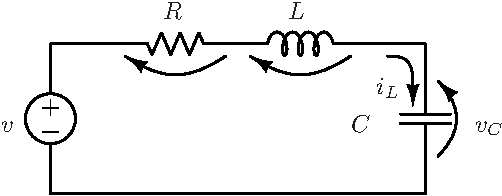
\includegraphics{rlc-serie.pdf}
  \caption{Circuito RLC serie (Ejercicio~\ref{RLC-serie}).}
  \label{fig:rlc-serie}
\end{figure}

\begin{enumerate}
  \item Observar que el sistema es equivalente al oscilador armónico del Ejercicio \ref{oscilador-armonico}. ¿Qué papel juega cada componente del circuito eléctrico?
  \item Realizar diagramas de fase para los siguientes casos: 
  \begin{itemize}
    \item \emph{no-amortiguado}: $R=0$,
    \item \emph{sub-amortiguado}: $\Delta<0$,
    \item \emph{amortiguamiento crítico:} $\Delta=0$,
    \item \emph{sobre-amortiguado:} $\Delta>0$.
  \end{itemize}
  \item Interpretar los gráficos obtenidos. 
\end{enumerate}
\end{ejer}


%----------------------------------------------------------
% 21

\begin{ejer}[Péndulo]\label{pendulo} Se considera el problema del péndulo:
$$\left\{\begin{array}{ll}
\ddot{\theta}(t)=-A\sen( \theta(t)) -b\dot{\theta}\mbox{ en } [0,T]\\
\dot{\theta}(0) = v_0 \\
\theta(0)=\theta_0 
\end{array}\right.$$
donde $\theta$ representa el ángulo que forma la vara del péndulo con la vertical.

\begin{enumerate}
\item Formular el problema como un sistema de ecuaciones de orden uno.
\item Realizar diagramas de fase y comparar con el caso lineal (e.g.: el Ejercicio \ref{RLC-serie}). 
\end{enumerate}
\end{ejer}

%----------------------------------------------------------
% 22
\begin{ejer} Realizar un diagrama de fases 3D del sistema dado por el modelo SIR del Ejercicio \ref{modelo-SIR}\end{ejer}


%----------------------------------------------------------
% 23
\begin{ejer}[Problema de tres cuerpos]
Se quiere resolver el problema de tres cuerpos, sujetos a atracción gravitatoria mutua. Para simplificar, supondremos que los cuerpos se mueven en un mismo plano. Si notamos $r_i = (x_i,y_i)$ la posición del cuerpo $i$-ésimo, y $m_i$ su masa ($i=1,2,3$), las ecuaciones (vectoriales) que rigen el movimiento de los cuerpos son:
\begin{equation}\label{eq:gravitacion}
\ddot{r_1} = -G m_2 \frac{r_2-r_1}{\|r_1-r_2\|^3}-G m_3\frac{r_3-r_1}{\|r_3-r_1\|^3},
\end{equation}
para el primer cuerpo, y las análogas para los otros dos. $G$ es la constante de gravitación universal, $G=0.4982 \frac{\textrm{m}^3}{\textrm{dia}^2\textrm{Kg}}$. 
\begin{enumerate}
\item Formular el problema como un sistema de orden uno de la forma: 
$$\dot{u}=f(u).$$
Observar que deben obtenerse doce ecuaciones ($u\in\R^{12}$): cada una de las tres ecuaciones vectoriales de la forma \eqref{eq:gravitacion} debe escribirse como dos ecuaciones escalares (una por coordenada), y a su vez, estas ecuaciones de segundo orden se convierten en dos de orden uno. Para la implementación, tener en cuenta que no es necesario mantener la forma de vector. Es decir: puede tomarse $u\in\R^{3\times 4}$, por ejemplo, sin que esto genere inconvenientes para el solver.
\item Implementar una función \lstinline{tres_cuerpos(t, u, m1, m2, m3)} que devuelva la derivada del estado. 
\item Se desea resolver el problema para el sistema Sol (S) - Tierra (T)- Luna (L). Las masas de estos cuerpos (en Kg) son: $m_T = 5.97\times 10^{24}$, $m_L = 7.3477\times10^{22}$ y $m_S = 1.9891\times10^{30}$. La distancia Tierra-Sol es $d_{TS} = 1.49597887\times10^{11}$m, y la distancia Tierra-Luna: $d_{TL} = 3.844\times 10^8$m. Supondremos que inicialmente el Sol se encuentra en el origen de coordenadas, la Tierra en el punto $(0,d_{TS})$ y la Luna en el punto $(d_{TS},d_{TL})$. 

La velocidad tangencial de la Tierra en torno del Sol, en metros/día, está dada por $v_T=\frac{2\pi d_{TS}}{365}$. Análogamente, la velocidad de la Luna tiene dos componentes: una corres\-pondiente a la rotación en torno al Sol, que se puede aproximar por $v_{LS} = v_T$, y otra correspondiente a su rotación entorno a la Tierra, dada por: $v_{LT}=\frac{2\pi d_{TL}}{28}$. Así, dadas las posiciones iniciales asumidas, las velocidades iniciales pueden tomarse: $v_S=(0,0)$, $v_T = (0,v_T)$ y $v_L = (-v_{LT},v_{LS})$. 

Con las masas y datos iniciales dados resolver las ecuaciones en un intervalo de tiempo que abarque $365$ días. 

\item Realizar una animación a partir de los resultados obtenidos. 
\end{enumerate}
\end{ejer}





%----------------------------------------------------------
% 24
\begin{ejer}
Mediante la confección de diagramas de fase adecuados, mostrar que el siguiente sistema tiene una bifurcación de Hopf en $\mu=0$.\
\[\left\{ \begin{array}{lcr}
    \dot{x} &=& y+\mu x-xy^2, \\
    \dot{y} &=& \mu y - x - y^3.
\end{array}\right.\]

\end{ejer}



%----------------------------------------------------------
% 25
\begin{ejer} 
Considerar la ecuación (escalada) $\dot{n} = (n+n_0)(1-n)-\frac{\alpha n^\gamma}{\beta+n^\gamma}$ utilizada por Boccara para modelar el crecimiento de pandillas callejeras (todos los parámetros son positivos). El primer término corresponde al crecimiento logístico con equilibrio desplazado del origen, mientras que el segundo corresponde a la respuesta social: es creciente con $n$, pero tiene un cierto límite. El parámetro $\gamma$ modula la \emph{dureza} de la respuesta social (¿Por qué?). 
\begin{enumerate}
\item Fijar un valor de $\gamma$ y un valor de $n_0$ y graficar conjuntamente $p(n) = (n+n_0)(1-n)$ y $g(n)=\frac{\alpha n^\gamma}{\beta+n^\gamma}$ para distintos valores de $\alpha\in(0;0.5)$ y $\beta\in(0;0.5)$. ¿Qué se observa? ¿Será posible que el sistema tenga dos equilibrios?
\item Elegir combinaciones de $\alpha$ y $\beta$ que representen distintos comportamientos y realizar los diagramas de fase correspondientes. Interpretar.
\end{enumerate}
\end{ejer}
%----------------------------------------------------------
% 26
\begin{ejer}
Resolver para distintos datos iniciales el oscilador de Van der Pol, dado por la ecuación: $\ddot{x}=\mu(1-x^2)\dot{x}+x$. Graficar las soluciones conjuntamente en el plano $(x,\dot{x})$. ¿Qué se observa? 

Repetir los gráficos para distintos valores de $\mu$ y analizar el efecto de la variación de $\mu$ en el comportamiento del sistema. 
\end{ejer}
%-----------------------------------------------------------
% 27

\begin{ejer} Considerar las ecuaciones: 
    \begin{itemize}
        \item $\dot{x} = \mu - x^2$
        \item $\dot{x} = \mu x - x^2$
        \item $\dot{x} = \mu x - x^3$
    \end{itemize}
    Graficar soluciones en el plano $(t,x)$ para distintos valores del parámetro $\mu$ ($\mu<0$, $\mu=0$ y $\mu>0$).
\end{ejer}

%----------------------------------------------------------
% 28
\begin{ejer} Considerar el modelo de Holling-Tanner 
\[\begin{array}{rcl}
\dot{x}&=&x\Big(1-\frac{x}{7}\Big) -\frac{xy}{7+7x} \\ 
\dot{y}&=&0.2y\Big(1-\frac{Ny}{x}\Big).
\end{array}\]
\begin{enumerate}
\item Hallar los equilibrios para $N=0.5$. Linealizar en torno a los equilibrios y esbozar los diagramas de fase del problema linealizado. 
\item Graficar un diagrama de fases del problema no lineal utilizando. Comparar. 
\end{enumerate}
\end{ejer} 

%----------------------------------------------------------
% 29
\begin{ejer} Considerar el siguiente sistema, propuesto por R\"ossler:
\[\left\{\begin{array}{rcl}
        \dot{x} &=& -y-z \\
        \dot{y} &=& x+ay \\
        \dot{z} &=& b+xz-cz,
        \end{array}\right.\]
donde $a,b,c$ son constantes. Tomar $a=b=0.2$ y $x_0=y_0=z_0=1$. 
\begin{enumerate}
    \item Para $c=2.3$, hallar y graficar un ciclo límite. Para ello, resolver el sistema para un tiempo relativamente largo y luego volver a resolver tomando como dato inicial el último punto de la trayectoria anterior. Graficar las tres componentes de la solución y graficar el ciclo en $\R^3$. De yapa, puede calcularse el período del ciclo detectando con un evento los cruces de un plano fijo.
    \item Repetir el experimento para $c=3.3$.
    \item Repetir el experimento para $c=6.3$. ¿Se alcanza un ciclo límite en este caso?
    \item Para $c=6.3$ resolver también para $x_0=1.01$, $y_0=z_0=1$ y comparar (por separado) las componentes $x$, $y$ y $z$ de esta solución perturbada con la solución original, con dato $x_0=y_0=z_0=1$. 
\end{enumerate}
\end{ejer}

\begin{ejer}[Lorenz]
El sistema de Lorenz está dado por las ecuaciones:
\[\left\{\begin{array}{rcl}
    \dot{x} &=& \sigma(y-x) \\
    \dot{y} &=& rx-y-xz \\
    \dot{z} &=& xy-bz,
    \end{array}\right.\]
donde asumiremos $\sigma=10$, $b=\frac{8}{3}$. 
\begin{enumerate}
    \item Observar que para $0<r<1$ hay un único punto crítico, en el origen. Realizar algunos diagramas de fase para este caso. 
    \item Realizar un diagrama de fases para el caso $r=1$ y para $r=2$.
    \item Para $r=15$ buscar un ciclo límite inestable. Para ello, invertir el tiempo integrando en el intervalo \lstinline{t_span=(10.0, 0.0)} (o, equivalentemente, cambiando el signo del campo).
    \item Resolver para $r=25$ y graficar la solución. Como en el ejercicio anterior: de ser necesario reiniciar la resolución a partir del final de la simulación previa para así encontrar el atractor de Lorenz.
    \item Para $r=28$, resolver con dos datos iniciales que difieran en $10^{-8}$ y graficar la diferencia entre las dos soluciones en escala logarítmica. ¿Cuánto tarda en volverse de orden $1$? Este es el fenómeno de sensibilidad a las condiciones iniciales que hace que, en dimensión tres, el Teorema de Poincaré--Bendixson no tenga análogo.
    \item De yapa: hacer una animación en la que un punto se mueva a lo largo de la trayectoria al tiempo que la va dibujando. 
\end{enumerate}
\end{ejer}

\subsection*{Laboratorio: los problemas conductores}

\begin{ejer}[Ajuste del modelo SIR a datos]\label{lab:SIR-ajuste}
Se dispone de una serie temporal de casos diarios de una epidemia (el archivo se provee con el notebook correspondiente; también puede usarse cualquier serie pública de casos de gripe o de COVID-19 de una ciudad durante una única ola).
\begin{enumerate}
\item Implementar el modelo SIR y una función que, dados $(\beta,\gamma,i_0)$, devuelva la curva de nuevos casos diarios $\beta s i N$ evaluada en los días de los datos.
\item Ajustar $(\beta,\gamma,i_0)$ por mínimos cuadrados (\lstinline{scipy.optimize.least_squares} o \lstinline{curve_fit}) usando sólo la primera mitad de la serie. Graficar el ajuste junto con los datos y los residuos.
\item Con los parámetros ajustados, predecir la segunda mitad de la serie y compararla con los datos reales. ¿Predice bien el pico? ¿Y la cola?
\item Repetir el ajuste desde varios puntos iniciales del optimizador. ¿Se obtienen siempre los mismos parámetros? ¿Y el mismo $R_0=\beta/\gamma$? Interpretar: ¿qué combinaciones de parámetros determinan los datos y cuáles no?
\item Repetir con el modelo SEIR (Ejercicio \ref{modelo-SEIR}). ¿Mejora el ajuste? ¿Cambia la predicción?
\item Escribir un párrafo con la conclusión: qué puede decir el modelo sobre esta epidemia y qué no.
\end{enumerate}
\end{ejer}

\begin{ejer}[La forma de onda del circuito de van der Pol]
\begin{enumerate}
\item Resolver \eqref{eq:vdP-sistema} para $\lambda = 0.1, 1, 5, 20$ con dato inicial $(0.01,0)$ y tiempo suficiente para llegar al ciclo límite. Graficar $x(t)$ en régimen permanente para cada $\lambda$ y describir cómo cambia la forma de onda.
\item Medir numéricamente la amplitud y el período del ciclo en función de $\lambda$ (usar un evento para detectar los cruces por $x=0$). Comparar la amplitud con la predicción $2$ del Ejercicio \ref{ejer:vdP-guiado} y el período con $2\pi$ para $\lambda$ chico. ¿Cómo crece el período para $\lambda$ grande?
\item Calcular el espectro de $x(t)$ en régimen permanente (\lstinline{numpy.fft}) para $\lambda=0.1$ y $\lambda=5$. ¿Cuántos armónicos son apreciables en cada caso? (Este ítem anticipa la Parte II.)
\item \emph{Problema inverso.} Se provee un registro de corriente con ruido (o se lo genera sumando ruido a una simulación con $\lambda$ desconocido). Estimar $\lambda$ a partir del registro, por ejemplo minimizando la distancia entre la forma de onda medida y la simulada. Discutir qué característica del registro (amplitud, período, forma) es más sensible a $\lambda$.
\end{enumerate}
\end{ejer}


\part{Análisis de Fourier}
\chapter{Introducción}\label{cap:intro-II}

El análisis de Fourier ocupa un lugar central en la matemática aplicada, la física y, de manera cada vez más visible, en la ciencia de datos y el procesamiento de señales. Su idea fundamental --descomponer una señal, función o conjunto de datos en componentes elementales asociadas a distintas frecuencias-- proporciona un lenguaje poderoso para describir, analizar y manipular fenómenos complejos.

Estas notas están pensadas como una introducción al análisis de Fourier con énfasis en las aplicaciones y busca tender un puente entre los aspectos teóricos esenciales y su uso efectivo en problemas concretos. En particular, el objetivo no es desarrollar la teoría en su máxima generalidad ni con el mayor grado de abstracción posible, sino presentar los conceptos clave de manera clara, acompañados de ejemplos, interpretaciones y aplicaciones relevantes.

\section{Motivación}

Muchas de las señales que aparecen en la práctica --datos experimentales, registros temporales, imágenes, soluciones de ecuaciones diferenciales-- presentan estructuras oscilatorias o periódicas. En este contexto, resulta natural preguntarse si es posible describir dichas señales como superposiciones de oscilaciones más simples, y qué información se puede extraer de esa descomposición.

El análisis de Fourier responde a estas preguntas mostrando que, bajo hipótesis bastante generales, una función puede representarse como una suma (o integral) de funciones elementales oscilatorias. Esta perspectiva frecuencial permite:
\begin{itemize}
\item identificar escalas dominantes en una señal,
\item separar información relevante de ruido,
\item diseñar filtros para modificar o mejorar datos,
\item y resolver ecuaciones diferenciales mediante técnicas sistemáticas.
\end{itemize}

Desde el punto de vista de la ciencia de datos, la transformada de Fourier constituye una herramienta básica para el análisis exploratorio, el preprocesamiento de datos y la compresión de información.

\section{Problema conductor: una serie temporal de temperatura}\label{sec:conductor-senal}

Para fijar ideas, tomemos una señal concreta que nos va a acompañar en toda esta parte: el registro de la temperatura del aire en una estación meteorológica, medida cada hora durante varios años. Es una serie de unos $8760$ valores por año, que a simple vista muestra dos oscilaciones superpuestas, una diaria y una anual, más una cantidad importante de variabilidad que no sigue ningún patrón evidente (frentes, tormentas, ruido de medición). Sobre esta señal queremos responder:
\begin{enumerate}
\item ¿Qué frecuencias contiene? ¿Con qué amplitud y con qué fase contribuye cada una? ¿Cuánto de la variabilidad total explican el ciclo diario y el anual?
\item ¿Cómo separar la parte ``regular'' de la señal (los ciclos) de la parte irregular, y qué queda cuando se lo hace?
\item Si en lugar de una medición por hora tuviéramos una por día, o una por semana, ¿qué información se pierde y qué información \emph{se falsea}?
\item ¿Cuántos números hacen falta para reconstruir la señal con un error dado? ¿Se puede comprimir?
\item Las herramientas que sirven para esta señal, ¿sirven igual para un audio, un electrocardiograma o una imagen?
\end{enumerate}
La misma señal reaparece en la Parte III: la temperatura en la superficie del suelo es la ``condición de borde'' que fuerza la difusión del calor hacia abajo, y lo que aprendamos sobre su contenido de frecuencias va a determinar qué tan profundo llega cada ciclo.

\figpendiente{Serie horaria de temperatura}{Un año de temperatura horaria (datos reales de una estación meteorológica), con un zoom sobre una semana para ver el ciclo diario.}

\section{Contenido del curso}

El recorrido que proponemos comienza con las {\em series de Fourier}, que permiten representar funciones periódicas como sumas infinitas de senos y cosenos. Este caso discreto y relativamente concreto sirve como laboratorio para introducir ideas fundamentales como:
\begin{itemize}
\item distintos tipos de convergencia (puntual, uniforme y en norma ($L^2$)),
\item el papel de la ortogonalidad,
\item y las limitaciones inherentes a estas representaciones, ilustradas de manera paradigmática por el {\em fenómeno de Gibbs}.
\end{itemize}

A continuación, pasamos a la {\em transformada de Fourier}, que extiende estas ideas al caso no periódico. Veremos su definición, propiedades básicas y la {\em fórmula de inversión}, poniendo especial atención en su interpretación y en las condiciones bajo las cuales los resultados son válidos.

En una segunda etapa, abordaremos la {\em transformada discreta de Fourier (DFT)} y el algoritmo de la {\em Transformada rápida de Fourier (FFT)}, que permiten llevar estas ideas al terreno computacional. Aquí el foco estará en la implementación eficiente, la complejidad algorítmica y la conexión entre los objetos matemáticos continuos y sus contrapartes discretas.

Finalmente, exploraremos algunas aplicaciones relevantes, entre ellas:
\begin{itemize}
\item procesamiento de señales y filtrado,
\item técnicas básicas de {\em denoising},
\item y aplicaciones a la resolución de ecuaciones en derivadas parciales, donde el análisis de Fourier aparece como una herramienta natural para desacoplar variables y entender la estructura de las soluciones.
\end{itemize}

\section{Enfoque y nivel de rigor}

A lo largo de las notas se presentarán demostraciones de varios resultados importantes, en algunos casos con un nivel de detalle cercano al rigor matemático estándar. Sin embargo, el énfasis estará puesto en la comprensión conceptual y en la utilidad de los resultados más que en la completitud formal.

Cuando sea apropiado, se privilegiarán argumentos intuitivos, ejemplos explícitos y visualizaciones, con el objetivo de que el lector adquiera una buena intuición del significado de los conceptos introducidos. El lector interesado en un tratamiento completamente riguroso encontrará abundante bibliografía para profundizar.

En resumen, estas notas buscan ofrecer una primera aproximación sólida y operativa al análisis de Fourier, que permita tanto comprender sus fundamentos matemáticos como aplicarlos con confianza en problemas reales de ciencia de datos y matemática aplicada.


\chapter{Series de Fourier}

Las series de Fourier fueron introducidas a comienzos del siglo XIX por Joseph Fourier en su estudio de la ecuación de la difusión (o ecuación del calor). En su {\em Théorie analytique de la chaleur} en 1822 \cite{Fourier}, Fourier propuso representar funciones periódicas como sumas infinitas de senos y cosenos, con el objetivo de describir la evolución temporal de la temperatura en un sólido. Esta idea, inicialmente motivada por un problema físico concreto, resultó ser extraordinariamente fecunda y abrió el camino a una nueva forma de analizar funciones mediante su contenido frecuencial.

A partir de esta propuesta surgieron desarrollos fundamentales en numerosas áreas de la matemática pura y aplicada, incluyendo el análisis armónico, la teoría de funciones, la teoría de espacios funcionales y la resolución de ecuaciones en derivadas parciales. En la actualidad, las series de Fourier constituyen una herramienta central no solo en física e ingeniería, sino también en procesamiento de señales, ciencia de datos y aprendizaje automático, donde permiten descomponer, analizar y manipular información compleja de manera sistemática.

\section{Ondas fundamentales}\label{sec:ondas-fundamentales}

La idea central de las series de Fourier consiste en buscar descomponer una señal temporal \(x(t)\) como superposición de oscilaciones armónicas simples. Pero, ¿qué entendemos exactamente por una de estas oscilaciones?

Llamaremos {\em onda fundamental} a una oscilación armónica simple de la forma
$$
A\cos(\omega_0 t + \phi),
$$
donde $A$ es la amplitud, $\phi$ es la fase y $\omega_0 = 2\pi f$ es la frecuencia angular asociada a la frecuencia fundamental $f$. Esta última está relacionada con el {\em período} $T$ de la onda mediante la relación $T = 1/f$ (ver Figura~\ref{fig:ondas-fundamentales}).

\begin{figure}[ht]
  \centering
  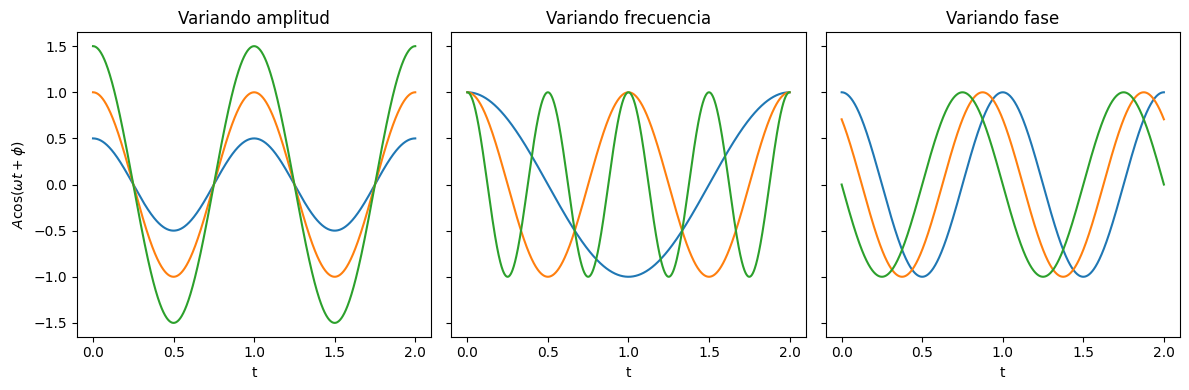
\includegraphics[width=0.8\textwidth]{ondas-fundamentales.png}
  \caption{Ondas fundamentales con distintas amplitudes, frecuencias y fases.}
  \label{fig:ondas-fundamentales}
\end{figure}

En efecto, observemos que
$$
\cos(\omega_0 (t+T) + \phi) = \cos(\omega_0 t + \phi + \omega_0 T) = \cos(\omega_0 t + \phi) \quad \Longleftrightarrow \quad \omega_0 T = 2k\pi,\ k\in\mathbb{Z}.
$$
El período fundamental corresponde al menor $T>0$ que satisface esta igualdad, es decir,
$$
T = \frac{2\pi}{\omega_0} = \frac{1}{f}.
$$
\begin{obs}[Unidades]
El argumento de una función trigonométrica debe ser adimensional. En particular, el producto $\omega_0 t$ no puede tener unidades, lo que implica que la frecuencia angular $\omega_0$ tiene unidades de inverso de tiempo. La frecuencia fundamental $f$ se mide en hertz (Hz), donde $1\,\mathrm{Hz} = 1\,\mathrm{s}^{-1}$, y se relaciona con la frecuencia angular mediante $\omega_0 = 2\pi f$. Aunque suele escribirse que $\omega_0$ se mide en rad/s, el radián es adimensional, por lo que desde el punto de vista dimensional $\omega_0$ tiene unidades $1/\mathrm{s}$.
\end{obs}

En la práctica, no siempre resulta conveniente trabajar explícitamente con la fase $\phi$. En muchos casos es más simple escribir una oscilación armónica como combinación de un coseno y un seno de la misma frecuencia.

En efecto, usando la identidad trigonométrica
$$
\cos(\alpha+\beta)=\cos\alpha\cos\beta-\sin\alpha\sin\beta,
$$
podemos escribir
$$
A\cos(\omega_0 t + \phi) = A\cos\phi\,\cos(\omega_0 t) - A\sin\phi\,\sin(\omega_0 t).
$$
Definiendo
$$
a = A\cos\phi, \qquad b = -A\sin\phi,
$$
obtenemos la representación equivalente
$$
A\cos(\omega_0 t + \phi) = a\cos(\omega_0 t) + b\sin(\omega_0 t).
$$

Recíprocamente, dados $a$ y $b$, la amplitud y la fase pueden recuperarse mediante
$$
A = \sqrt{a^2+b^2}, \qquad \tan\phi = -\frac{b}{a}.
$$

Una forma aún más compacta y conveniente de representar oscilaciones armónicas consiste en utilizar exponenciales complejas. Recordemos la identidad de Euler
$$
e^{i\theta} = \cos\theta + i\sin\theta,
$$
donde $i$ es la unidad imaginaria compleja ($i^2=-1$).

A partir de ella, se obtiene inmediatamente que
$$
\cos(\omega_0 t) = \Re\bigl(e^{i\omega_0 t}\bigr), \qquad \sin(\omega_0 t) = \Im\bigl(e^{i\omega_0 t}\bigr).
$$

En consecuencia, la combinación lineal
$$
a\cos(\omega_0 t) + b\sin(\omega_0 t)
$$
puede escribirse como la parte real de una exponencial compleja. En efecto,
$$
a\cos(\omega_0 t) + b\sin(\omega_0 t) = \Re\bigl((a - ib)e^{i\omega_0 t}\bigr).
$$

De este modo, toda oscilación armónica de frecuencia $\omega_0$ puede representarse mediante una única exponencial compleja $c\, e^{i\omega_0 t}$, donde $c = a- ib$ es un número complejo que codifica simultáneamente la amplitud y la fase de la onda. Esta representación resulta especialmente conveniente en el desarrollo de las series de Fourier y será utilizada de manera sistemática en lo que sigue.

Observemos que si representamos una oscilación armónica mediante una exponencial compleja de la forma
$$
c\,e^{i\omega_0 t},
$$
entendiendo que la señal física corresponde a su parte real, el número complejo $c$ codifica de manera directa la amplitud y la fase de la onda. En efecto, escribiendo $c$ en forma polar como
$$
c = A\,e^{i\phi}, \quad (A=|c|,\ \phi=\arg(c))
$$
se obtiene
$$
\Re\bigl(c\,e^{i\omega_0 t}\bigr) = A \cos(\omega_0 t + \phi).
$$
De este modo, el módulo $A=|c|$ representa la amplitud de la onda, mientras que el argumento $\arg(c)=\phi$ coincide con su fase.

\section{Superposición de ondas fundamentales}

Tomemos una serie temporal $f\colon \R\to\C$ y supongamos que tiene período $L$ (ver Figura \ref{fig:sombrero}).

\begin{figure}[ht]
  \centering
  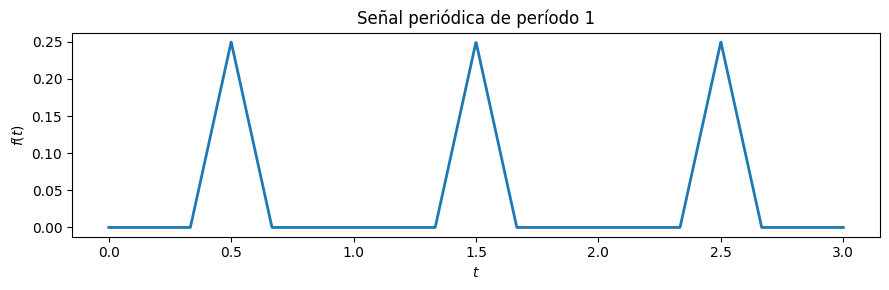
\includegraphics[width=0.7\textwidth]{sombrero.png}
  \caption{Ejemplo de señal periódica.}
  \label{fig:sombrero}
\end{figure}

Queremos representar esta señal como una superposición de ondas fundamentales. Entonces no cualquier frecuencia es compatible con esta periodicidad. En efecto, consideremos una onda compleja de la forma
$$
e^{i\omega t}.
$$
Para que esta función sea $L-$periódica debe cumplirse que
$$
e^{i\omega(t+L)} = e^{i\omega t} \quad \text{para todo } t.
$$
Esto equivale a exigir
$$
e^{i\omega L} = 1,
$$
lo cual ocurre si y solo si
$$
\omega L = 2k\pi, \qquad k \in \Z.
$$
\begin{figure}[ht]
  \centering
  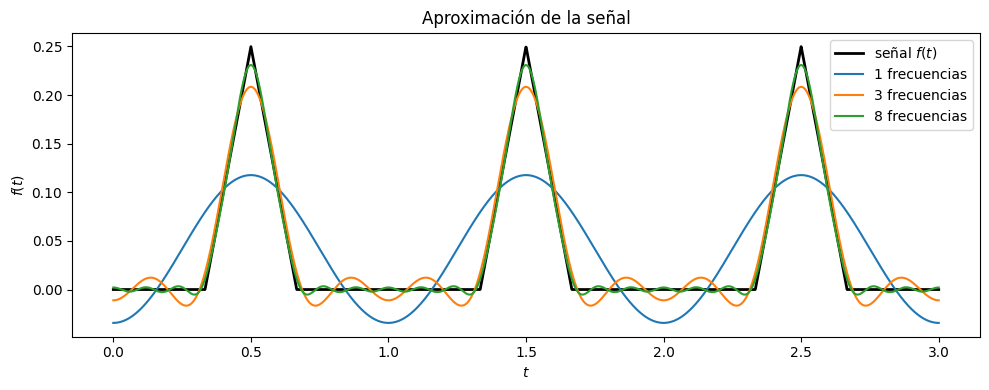
\includegraphics[width=0.7\textwidth]{sombrero-aproximacion.png}
  \caption{Aproximación de la señal superponiendo 1, 3 y 8 frecuencias.}
  \label{fig:sombrero-aproximacion}
\end{figure}
En consecuencia, las únicas frecuencias angulares compatibles con una periodicidad $L$ son
$$
\omega_k = \frac{2k\pi}{L}, \qquad k \in \Z.
$$
Estas frecuencias discretas constituyen los modos fundamentales de oscilación asociados al período $L$. Cualquier combinación de ondas de este tipo será nuevamente $L-$periódica, y serán precisamente estas frecuencias las que aparecerán en el desarrollo en series de Fourier de una función periódica.

Luego, buscamos construir una aproximación de la señal $f(t)$ de la forma
$$
f(t) \sim \sum c_k e^{i\omega_k t} = \sum c_k e^{i \frac{2k\pi}{L} t}.
$$
Ver la Figura \ref{fig:sombrero-aproximacion} para ver las aproximaciones conseguidas usando $1$, $3$ y $8$ frecuencias fundamentales.

\section{Ortogonalidad}

Antes de introducir la noción de coeficientes de Fourier, conviene recordar brevemente cómo se calculan las coordenadas de un vector en un espacio finito-dimensional cuando se dispone de una base ortogonal.

\subsection{Un repaso finito-dimensional}

Sea $\{v_1,\dots,v_n\}$ una base ortogonal de $\R^n$ (no necesariamente ortonormal), es decir,
$$
\langle v_i, v_j\rangle = 0 \quad \text{si } i\neq j.
$$
Todo vector $\xx\in\R^n$ puede escribirse de manera única como
$$
\xx = \sum_{k=1}^n c_k v_k.
$$
Tomando producto interno con $v_j$ y usando la ortogonalidad, obtenemos
$$
\langle \xx, v_j\rangle = c_j \langle v_j, v_j\rangle,
$$
de donde se deduce inmediatamente
$$
c_j = \frac{\langle \xx, v_j\rangle}{\langle v_j, v_j\rangle}.
$$
Este procedimiento muestra que, cuando la base es ortogonal, el cálculo de las coordenadas se desacopla completamente: cada coeficiente se obtiene proyectando el vector sobre un único vector de la base.

\subsection{De vectores a funciones: una motivación}

La idea central de las series de Fourier es extender este mecanismo al caso de funciones. Para motivar la noción de ortogonalidad entre funciones, pensemos primero en una aproximación discreta.

Supongamos que tenemos dos funciones complejas $f(t)$ y $g(t)$ definidas en un intervalo $[0,L]$ a valores en $\C$. Si tomamos una partición uniforme
$$
t_j = \frac{jL}{N}, \qquad j=0,\dots,N-1,
$$
podemos asociar a cada función el vector en $\C^N$
$$
\bigl(f(t_0), f(t_1), \dots, f(t_{N-1})\bigr),\ \bigl(g(t_0), g(t_1), \dots, g(t_{N-1})\bigr).
$$
En este contexto discreto, una noción natural de producto interno es
$$
\langle f, g\rangle_N = \frac{1}{N}\sum_{j=0}^{N-1} f(t_j)\,\overline{g(t_j)}.
$$
Si, al aumentar $N$, estos productos internos tienden a cero, diremos informalmente que las funciones son ortogonales. Este razonamiento sugiere definir, en el límite continuo, el producto interno
\begin{equation}\label{pi.L2}
\langle f, g\rangle = \frac{1}{L}\int_0^L f(t)\,\overline{g(t)}\,dt,
\end{equation}
que será la noción fundamental de ortogonalidad entre funciones periódicas de período $L$.

\section{Definición de series de Fourier}

Motivados por la discusión de la sección anterior, consideremos ahora el conjunto de funciones
\begin{equation}\label{def:ek}
e_k(t) = e^{i\omega_k t}, \qquad  \omega_k = \frac{2\pi k}{L}, \quad k\in\Z.
\end{equation}
Es decir, el conjunto de las ondas fundamentales complejas en el intervalo $[0, L]$.

Tenemos el siguiente resultado
\begin{prop} Sea $e_k(t)$ dado por \eqref{def:ek}. Entonces el conjunto $\{e_k\}_{k\in\Z}$ resulta ortogonal respecto al producto interno dado por \eqref{pi.L2}.
\end{prop}

\begin{proof}
Un cálculo directo muestra que
$$
\langle e_k, e_m\rangle = \frac{1}{L}\int_0^L e^{i(\omega_k-\omega_m)t}\,dt =
\begin{cases}
1, & k=m,\\
0, & k\neq m.
\end{cases}
$$
Es decir, las funciones $e^{i\omega_k t}$ forman un conjunto ortogonal (de hecho, ortonormal) con respecto a este producto interno.
\end{proof}


Motivados por el caso finito-dimensional, si una función periódica $f$ puede escribirse formalmente como
$$
f(t) \sim \sum_{k\in\Z} c_k\, e^{i\omega_k t},
$$
la ortogonalidad permite calcular cada coeficiente de manera independiente:
\begin{equation}\label{coef.fourier}
c_k = \langle f, e_k\rangle = \frac{1}{L}\int_0^L f(t)\,e^{-i\omega_k t}\,dt.
\end{equation}
Esta fórmula es el análogo funcional de la expresión de las coordenadas de un vector en una base ortogonal y constituye el punto de partida del análisis de Fourier.

\begin{defi}
Sea $f\colon \R\to\C$ una señal periódica de período $L$. Definimos los {\em coeficientes de Fourier} de $f$ a 
$$
c_k(f) = \hat f[k] = c_k = \frac{1}{L}\int_0^L f(t)\,e^{-i\omega_k t}\,dt =\frac{1}{L}\int_{-\frac{L}{2}}^{\frac{L}{2}} f(t)\,e^{-i\omega_k t}\,dt
$$
\end{defi}

\begin{defi}
Se define la {\em serie de Fourier} de $f$ a la expresión formal
$$
S[f](t) = \sum_{k\in\Z} c_k\, e^{i\omega_k t},
$$
donde $\omega_k = \frac{2k\pi}{L}$ y $c_k$ viene dado por \eqref{coef.fourier}.
\end{defi}


\subsection{De la representación compleja a senos y cosenos}\label{complejo.a.real}

Hasta ahora hemos trabajado con la representación compleja de una función periódica,
$$
f(t) \sim \sum_{k\in\Z} c_k\, e^{i\omega_k t}, \qquad \omega_k = \frac{2\pi k}{L}.
$$
Esta formulación es particularmente conveniente desde el punto de vista algebraico y conceptual. Sin embargo, en muchas aplicaciones —y en particular cuando la señal $f$ es real— resulta natural buscar una representación enteramente real.

Si $f(t)$ es real para todo $t$, entonces los coeficientes complejos satisfacen la relación de simetría
$$
c_{-k} = \overline{c_k}, \qquad k\in\Z.
$$
En efecto
\begin{align*}
\overline{c_k} &= \overline{\frac{1}{L}\int_0^L f(t)\,e^{-i\frac{2k\pi}{L} t}\,dt}\\
& = \frac{1}{L}\int_0^L f(t)\,\overline{e^{-i\frac{2k\pi}{L} t}}\,dt\\
& =  \frac{1}{L}\int_0^L f(t)\,e^{i\frac{2k\pi}{L} t}\,dt\\
&= c_{-k}
\end{align*}

Esta propiedad garantiza que la suma compleja sea real y permite reagrupar los términos correspondientes a las frecuencias $\pm k$.

En efecto, para $k\geq 1$,
$$
c_k e^{i\frac{2k\pi}{L} t} + c_{-k} e^{-i\frac{2k\pi}{L} t} = c_k e^{i\frac{2k\pi}{L} t} + \overline{c_k} e^{-i\frac{2k\pi}{L} t} = 2\,\Re\bigl(c_k e^{i\frac{2k\pi}{L} t}\bigr).
$$
Escribiendo $c_k = \alpha_k - i\beta_k$ con $\alpha_k,\beta_k\in\R$, se obtiene
$$
2\,\Re\bigl(c_k e^{i\omega_k t}\bigr) = 2\alpha_k \cos(\omega_k t) + 2\beta_k \sin(\omega_k t).
$$

De este modo, toda función real y periódica puede escribirse como una serie de senos y cosenos:
$$
f(t) \sim \frac{a_0}{2} + \sum_{k=1}^\infty \Bigl( a_k \cos(\omega_k t) + b_k \sin(\omega_k t) \Bigr),
$$
donde los coeficientes reales están relacionados con los coeficientes complejos por
$$
a_0 = 2\, c_0, \qquad a_k = 2\,\Re(c_k), \qquad b_k = -2\,\Im(c_k), \quad k\geq 1.
$$

\subsection{De la representación real a la compleja}\label{real.a.complejo}

Recíprocamente, dada una representación real en términos de senos y cosenos,
$$
f(t) \sim \frac{a_0}{2} + \sum_{k=1}^\infty \Bigl( a_k \cos(\omega_k t) + b_k \sin(\omega_k t) \Bigr),
$$
puede recuperarse la forma compleja escribiendo
$$
\cos(\omega_k t) = \frac{e^{i\omega_k t}+e^{-i\omega_k t}}{2}, \qquad \sin(\omega_k t) = \frac{e^{i\omega_k t}-e^{-i\omega_k t}}{2i}.
$$
Un cálculo directo muestra entonces que
$$
c_k = \frac{1}{2}\bigl(a_k - i b_k\bigr), \qquad c_{-k} = \frac{1}{2}\bigl(a_k + i b_k\bigr), \quad k\geq 1,
$$
y $c_0 = \frac{a_0}{2}$.


En conclusión, las representaciones compleja y real de una serie de Fourier son completamente equivalentes. La elección de una u otra depende del contexto: la formulación compleja es más compacta y algebraicamente natural, mientras que la representación en términos de senos y cosenos resulta más transparente cuando se trabaja con señales reales.

\subsection{Ortogonalidad de senos y cosenos}

La ortogonalidad de las funciones seno y coseno puede deducirse directamente de la ortogonalidad de las exponenciales complejas. Recordemos que, para $k,m\in\Z$,
$$
\frac{1}{L}\int_0^L e^{i\omega_k t}\,\overline{e^{i\omega_m t}}\,dt = \frac{1}{L}\int_0^L e^{i(\omega_k-\omega_m)t}\,dt =
\begin{cases}
1, & k=m,\\
0, & k\neq m,
\end{cases}
$$
donde $\omega_k = \frac{2\pi k}{L}$.

Usando las identidades
$$
\cos(\omega_k t) = \frac{e^{i\omega_k t}+e^{-i\omega_k t}}{2}, \qquad \sin(\omega_k t) = \frac{e^{i\omega_k t}-e^{-i\omega_k t}}{2i},
$$
podemos expresar los productos de senos y cosenos en términos de productos de exponenciales.

Por ejemplo,
$$
\frac{1}{L}\int_0^L \cos(\omega_k t)\cos(\omega_m t)\,dt = \frac{1}{4}\sum_{\varepsilon,\eta=\pm1} \frac{1}{L}\int_0^L e^{i(\varepsilon\omega_k+\eta\omega_m)t}\,dt.
$$
Cada uno de estos términos se anula salvo cuando $\ve\omega_k+\eta\omega_m=0$, lo cual ocurre únicamente si $k=m$. En ese caso,
$$
\frac{1}{L}\int_0^L \cos^2(\omega_k t)\,dt = \frac{1}{2}.
$$
Por lo tanto,
$$
\frac{1}{L}\int_0^L \cos(\omega_k t)\cos(\omega_m t)\,dt =
\begin{cases}
\frac{1}{2}, & k=m\neq 0,\\
0, & k\neq m.
\end{cases}
$$

Un cálculo completamente análogo muestra que
$$
\frac{1}{L}\int_0^L \sin(\omega_k t)\sin(\omega_m t)\,dt =
\begin{cases}
\frac{1}{2}, & k=m,\\
0, & k\neq m,
\end{cases}
$$
mientras que
$$
\frac{1}{L}\int_0^L \sin(\omega_k t)\cos(\omega_m t)\,dt = 0 \qquad \text{para todo } k,m.
$$


En conclusión, el conjunto de funciones
$$
\left\{1,\ \cos(\omega_k t),\ \sin(\omega_k t)\right\}_{k\geq 1}
$$
es un conjunto ortogonal en el espacio de funciones periódicas de período $L$ con respecto al producto interno
$$
\langle f,g\rangle = \frac{1}{L}\int_0^L f(t)\,\overline{g(t)}\,dt.
$$

\section{Serie de Fourier real}

Cuando tenemos una señal real $f\colon \R\to\R$ entonces buscaremos su serie de Fourier de senos y cosenos.
\begin{defi}\label{trigo.fourier}
Sea $f\colon \R\to\R$ una función $L-$periódica. Su serie de Fourier en senos y cosenos se define como
$$
f(t)\sim S[f](t) = \frac{a_0}{2} + \sum_{k=1}^\infty a_k \cos(\tfrac{2k\pi}{L}t) + b_k \sin(\tfrac{2k\pi}{L}t),
$$
donde los coeficientes de Fourier, $a_k, b_k\in\R$ se definen como
\begin{align*}
&a_k = \frac{2}{L}\int_0^L f(t)\cos(\tfrac{2k\pi}{L}t)\, dt,\qquad k\in\N_0,\\
&b_k = \frac{2}{L}\int_0^L f(t)\sin(\tfrac{2k\pi}{L}t)\, dt,\qquad k\in\N.
\end{align*}
\end{defi}
La relación entre la serie de Fourier en senos y cosenos y la serie de Fourier compleja fue ya discutida en las secciones \ref{complejo.a.real} y \ref{real.a.complejo}.

\begin{volvemos}{la señal de temperatura}
Si suponemos que la temperatura $T(t)$ es, en primera aproximación, periódica de período $L=1$ año, la serie de Fourier real nos dice cómo escribirla como suma de oscilaciones: la componente $k$ tiene frecuencia $k$ ciclos por año, amplitud $A_k = \sqrt{a_k^2+b_k^2}$ y fase $\phi_k$, con $a_k\cos(\omega_kt)+b_k\sin(\omega_kt) = A_k\cos(\omega_k t+\phi_k)$ y $\tan\phi_k = -b_k/a_k$, como en la Sección \ref{sec:ondas-fundamentales}. El ciclo anual corresponde a $k=1$; el ciclo diario a $k=365$. La fase $\phi_1$ dice en qué día del año se alcanza la temperatura máxima media, y la amplitud $A_1$ cuánto difiere ese máximo de la media anual $a_0/2$. Esto responde, en principio, la primera pregunta de la Sección \ref{sec:conductor-senal}. Quedan dos dificultades, que son el tema de los capítulos siguientes: en qué sentido la serie ``recupera'' la señal (Capítulo \ref{chap:conv.Fourier}), y cómo calcular los coeficientes cuando en lugar de una función tenemos $8760$ números (Capítulo \ref{chap:DFT}).
\end{volvemos}

\chapter{Convergencia de la serie de Fourier}\label{chap:conv.Fourier}

Un problema matemático central en el análisis de Fourier es el estudio de la convergencia de la serie de Fourier y la determinación de las hipótesis bajo las cuales dicha serie recupera efectivamente la señal original.

El contenido de este capítulo será, en general, más riguroso que en los capítulos anteriores. En una primera lectura recomendamos al lector omitir las demostraciones y concentrarse en las aplicaciones de los resultados, regresando a los argumentos teóricos cuando se busque una comprensión más profunda.

\section{Propiedades de los coeficientes de Fourier}

Empecemos estudiando algunas propiedades generales que tienen los coeficientes de Fourier para una señal arbitraria $f\colon \R\to \C$. Sobre la señal $f$, sólo asumiremos en principio que es integrable, es decir que
$$
\int_0^L |f(t)|\, dt <\infty.
$$
Notaremos por $L^1([0,L])$ al conjunto de funciones integrables.

Si bien haremos todas las cuentas para los coeficientes de Fourier de la forma compleja \eqref{coef.fourier}, es un ejercicio sencillo adaptar los argumentos para tratar con los coeficientes en la forma trigonométrica dados por la Definición \ref{trigo.fourier}.

Empecemos con la siguiente proposición.
\begin{prop}\label{prop.coef}
Sea $f\in L^1([0,L])$ y $c_k=c_k(f)$ sus coeficientes de Fourier dados por \eqref{coef.fourier}. Entonces se tiene:
\begin{enumerate}
\item La sucesión $\{c_k\}_{k\in\Z}$ es acotada, i.e.
$$
|c_k|\le \frac{1}{L}\int_0^L |f(t)|\, dt.
$$

\item Si $f, g\in L^1([0,L])$ son dos señales, y $\lambda\in\C$, entonces
$$
c_k(f+g) = c_k(f)+c_k(g) \quad \text{y}\quad c_k(\lambda f) = \lambda c_k(f).
$$

\item Si $f$ es continua, diferenciable a trozos y $f'\in L^1([0,L])$, entonces
$$
c_k(f') = \frac{2k\pi i}{L}\, c_k(f).
$$

\item Si $f(t)\in\R$ y es par (i.e. $f(-t)=f(t)$), entonces $\Im(c_k)=0$ y
$$
c_k = \Re(c_k) = \frac{2}{L}\int_0^{\frac{L}{2}} f(t)\cos\left(\frac{2k\pi}{L}t\right)\, dt.
$$

\item Si $f(t)\in\R$ y es impar (i.e. $f(-t) = -f(t)$), entonces $\Re(c_k)=0$ y
$$
\frac{c_k}{i} = \Im(c_k) = \frac{2}{L}\int_0^{\frac{L}{2}} f(t)\sin\left(\frac{2k\pi}{L}t\right)\, dt.
$$
\end{enumerate}
\end{prop}

\begin{proof}
\begin{enumerate}
\item Este ítem es simple. En efecto, de \eqref{coef.fourier} tenemos
\begin{align*}
|c_k| &= \frac{1}{L}\left|\int_0^L f(t)\, e^{-i\frac{2k\pi}{L}t}\, dt \right|\le\frac{1}{L}\int_0^L \left|f(t)\, e^{-i\frac{2k\pi}{L}t}\right|\, dt \\
& = \frac{1}{L}\int_0^L |f(t)|\, dt.
\end{align*}

\item Este ítem es inmediato de la definición \eqref{coef.fourier} y de la linealidad de la integral.

\item Este ítem es una consecuencia de la fórmula de integración por partes, en efecto,
$$
c_k(f') = \frac{1}{L}\int_0^L f'(t)\, e^{-i\frac{2k\pi}{L}t}\, dt = \frac{1}{L}\left([f(t)\, e^{-i\frac{2k\pi}{L}t}]_0^L - \int_0^L f(t)\, \frac{d}{dt}e^{-i\frac{2k\pi}{L}t}\, dt\right).
$$
El término integrado es igual a 0 dado que $f(0)=f(L)$ (por la periodicidad y la continuidad de $f$; si $f$ es sólo diferenciable a trozos, se integra por partes en cada trozo y los términos de borde se cancelan por la continuidad). Como $\frac{d}{dt}e^{-i\frac{2k\pi}{L}t} = -\frac{2k\pi i}{L}e^{-i\frac{2k\pi}{L}t}$, obtenemos
$$
c_k(f') = \frac{2k\pi i}{L} \frac{1}{L}\int_0^L f(t)\, e^{-i\frac{2k\pi}{L}t}\, dt = \frac{2k\pi i}{L} c_k(f).
$$

\item Si $f$ es una función real y par, tenemos que
\begin{align*}
\int_0^L f(t)\, e^{-i\frac{2k\pi}{L}t}\, dt &= \int_{-\frac{L}{2}}^{\frac{L}{2}} f(t)\, e^{-i\frac{2k\pi}{L}t}\, dt\\
&=\int_{-\frac{L}{2}}^{\frac{L}{2}} f(t)\cos\left(\frac{2k\pi}{L}t\right)\, dt - i\int_{-\frac{L}{2}}^{\frac{L}{2}} f(t)\sin\left(\frac{2k\pi}{L}t\right)\, dt.
\end{align*}
Como $f$ es par y $\sin(\frac{2k\pi}{L}t)$ es impar, la segunda integral es 0 y como $\cos(\frac{2k\pi}{L}t)$ es par, tenemos que
$$
\int_{-\frac{L}{2}}^{\frac{L}{2}} f(t)\cos\left(\frac{2k\pi}{L}t\right)\, dt = 2\int_0^{\frac{L}{2}} f(t)\cos\left(\frac{2k\pi}{L}t\right)\, dt.
$$
Esto termina de probar lo deseado.

\item Este ítem es similar al anterior y omitimos la prueba.
\end{enumerate}
Con esto se concluye la demostración.
\end{proof}

Observemos que el punto 1 de la proposición anterior dice que los coeficientes de Fourier siempre están acotados. Combinando esto con el punto 3, obtenemos que si $f$ es continua y diferenciable a trozos con $f'$ integrable, 
$$
|c_k(f)| = \frac{L}{2k\pi}|c_k(f')|\le \frac{1}{2k\pi}\int_0^L |f'(t)|\, dt \to 0 \quad \text{cuando }k\to\infty.
$$
Esta propiedad sigue siendo cierta aún sin la hipótesis de ser diferenciable y se la conoce con el nombre de {\em Lema de Riemann-Lebesgue}.

\begin{lema}[Riemann-Lebesgue]\label{lema.RL}
Sea $f\in L^1([0,L])$, entonces
$$
\lim_{\lambda\to\infty}\int_0^L f(t)e^{i\lambda t}\, dt = 0.
$$
\end{lema}

\begin{proof}
Para la demostración usaremos el hecho de que las funciones $g\in C^1_c([0,L])$ son {\em densas} en el conjunto $L^1([0,L])$. Es decir que para todo $f\in L^1([0,L])$ y $\ve>0$, existe $f_\ve\in C^1_c([0,L])$ tal que
$$
\int_0^L |f(t)-f_\ve(t)|\, dt < \ve.
$$
La demostración de este hecho se encuentra en cualquier texto de teoría de la medida o teoría de integración. Ver, por ejemplo, \cite{Fava} o \cite{Zygmund}.

Ahora la prueba resulta muy similar al punto 3 de la proposición anterior. En efecto,
$$
\left|\int_0^L f(t)e^{i\lambda t}\, dt\right|\le \left|\int_0^L f_\ve(t)e^{i\lambda t}\, dt \right| + \int_0^L |f(t)-f_\ve(t)|\, dt < \left|\int_0^L f_\ve(t)e^{i\lambda t}\, dt \right| + \ve.
$$
Por otro lado, usando la fórmula de integración por partes,
$$
\int_0^L f_\ve(t)e^{i\lambda t}\, dt = \int_0^L f_\ve(t)\frac{1}{i\lambda}\frac{d}{dt}e^{i\lambda t}\, dt = -\frac{1}{i\lambda}\int_0^L f'_\ve(t) e^{i\lambda t}\, dt.
$$
Observemos que no aparece el término integrado dado que $f_\ve(0)=f_\ve(L)=0$. Luego, obtenemos
$$
 \left|\int_0^L f_\ve(t)e^{i\lambda t}\, dt \right| = \frac{1}{\lambda} \left|\int_0^L f'_\ve(t)e^{i\lambda t}\, dt \right|\le \frac{1}{\lambda}  \int_0^L |f_\ve'(t)|\, dt\to 0 \quad \text{cuando }\lambda\to\infty.
$$
Esto concluye la demostración.
\end{proof}

\section{Convergencia puntual de la serie de Fourier}

El primer resultado general sobre convergencia puntual de la serie de Fourier se remonta a Dirichlet, a comienzos del siglo XIX (1829). Este resultado fue posteriormente refinado por Jordan en 1881, quien obtuvo condiciones globales más generales sobre la señal $f$ que garantizan la convergencia puntual de la serie. De manera casi simultánea, hacia 1880, Dini formuló una condición puntual y muy general que asegura la convergencia de la serie de Fourier a $f$ en un punto dado $t_0$.

En este capítulo presentaremos la demostración del teorema de Dini. Este resultado proporciona una condición, formulada en términos del módulo de continuidad de la función, que permite garantizar la convergencia puntual de la serie de Fourier en un punto sin imponer hipótesis globales de suavidad.

\begin{teo}[Criterio de Dini de Convergencia puntual]\label{teo.Dini}
Sea $f\in L^1([0,L])$ una función $L$-periódica y sea $t_0$ un punto en el que existen los límites laterales $f(t_0^\pm)$ y tal que, llamando $S = \frac{f(t_0^+)+f(t_0^-)}{2}$,
\begin{equation}\label{Dini.cond}
\int_0^\delta \frac{|f(t_0+h)+f(t_0-h)-2S|}{h}\,dh < \infty
\end{equation}
para algún $\delta>0$. Entonces la serie de Fourier de $f$ converge en $t_0$ y
$$
\sum_{k\in\Z} c_k e^{i\omega_k t_0} = S = \frac{f(t_0^+)+f(t_0^-)}{2}.
$$
En particular, si $f$ es continua en $t_0$, $S=f(t_0)$ y la serie converge a $f(t_0)$.
\end{teo}

El caso que más se usa en la práctica es el siguiente.

\begin{cor}\label{cor.Dini-trozos}
Sea $f$ una función $L$-periódica, continua a trozos y con derivadas laterales en todo punto (por ejemplo, $f$ de clase $C^1$ a trozos). Entonces su serie de Fourier converge en todo punto $t_0$ al promedio de los límites laterales $\frac{f(t_0^+)+f(t_0^-)}{2}$; en particular converge a $f(t_0)$ en cada punto de continuidad.
\end{cor}

\begin{proof}
Si existen las derivadas laterales en $t_0$, existe $M$ tal que $|f(t_0+h)-f(t_0^+)|\le Mh$ y $|f(t_0-h)-f(t_0^-)|\le Mh$ para $0<h<\delta$, y entonces el integrando de \eqref{Dini.cond} está acotado por $2M$. Se aplica el Teorema \ref{teo.Dini}.
\end{proof}

\begin{obs}
Una función $f$ que verifica \eqref{Dini.cond} en un cierto $t_0$ se dice que verifica la {\em condición de Dini} en $t_0$.
\end{obs}

\begin{ejem}
Una pregunta importante es: ¿qué funciones verifican la condición de Dini \eqref{Dini.cond}? En los ejemplos que siguen $f$ es continua en $t_0$, de modo que $S=f(t_0)$.
\begin{enumerate}
\item El ejemplo más simple (y probablemente el más usado) es que si $f$ resulta diferenciable en $t_0$ entonces verifica la condición de Dini en $t_0$. En efecto, si $f$ es diferenciable en $t_0$ tenemos que
$$
\lim_{h\to 0} \frac{f(t_0+h)-f(t_0)}{h} = f'(t_0).
$$
En particular, tomando $M=|f'(t_0)|+1$, existe $\delta>0$ tal que si $|h|<\delta$, entonces
$$
|f(t_0+h)-f(t_0)|\le M|h|.
$$
Luego,
$$
\frac{|f(t_0+h)+f(t_0-h)-2f(t_0)|}{h}\le \frac{|f(t_0+h)-f(t_0)|}{h} + \frac{|f(t_0-h)-f(t_0)|}{h}\le 2M
$$
si $0<h<\delta$, y la condición de Dini \eqref{Dini.cond} se satisface.

\item La misma cuenta anterior muestra que si $f$ es {\em Lipschitz en $t_0$}, es decir
$$
|f(t)-f(t_0)|\le M |t-t_0|, \quad \text{para } |t-t_0|<\delta,
$$
entonces se verifica \eqref{Dini.cond}.

\item Un ejemplo del ítem 2 es la función $f(t) = |t|$. Esta función no es diferenciable en $t_0=0$ pero sí es Lipschitz en $t_0=0$. Por ende su serie de Fourier converge puntualmente en $t_0=0$.

\item Una generalización de este caso es cuando la función $f$ es {\em Hölder} $\alpha$ en $t_0$ ($0<\alpha<1$). Es decir, existe $0<\alpha<1$, $C>0$ y $\delta>0$ tales que
$$
|f(t_0+h)-f(t_0)|\le C|h|^\alpha \quad \text{para } |h|<\delta.
$$
Luego, razonando como en el ítem 1, obtenemos la desigualdad
$$
\int_0^\delta \frac{|f(t_0+h)+f(t_0-h)-2f(t_0)|}{h}\,dh \le 2C\int_0^\delta h^{\alpha-1}\, dh = \frac{2C\delta^\alpha}{\alpha}<\infty.
$$

\item Un ejemplo de una función Hölder es $f(t) = \sqrt[3]{t}$. Es fácil verificar que esta función no es diferenciable en $t_0=0$, tampoco es Lipschitz en $t_0=0$ pero es Hölder en $t_0=0$ con $\alpha=\frac13$.
\end{enumerate}
\end{ejem}


Veamos finalmente la demostración del Teorema de Dini. Es la parte más técnica del capítulo y puede omitirse en una primera lectura; lo que importa retener es el mecanismo: la suma parcial es una \emph{convolución} de $f$ con un núcleo (el núcleo de Dirichlet) que concentra su masa en el origen a medida que $N$ crece, y el Lema de Riemann--Lebesgue hace el resto.

\begin{proof}[Demostración del Teorema \ref{teo.Dini}]
Consideremos la $N-$ésima suma parcial de Fourier dada por
$$
S_N[f](t) = \sum_{k=-N}^N c_k\, e^{i\omega_k t},\qquad \omega_k = \frac{2k\pi}{L}.
$$
Queremos demostrar que $S_N[f](t_0)\to S$ cuando $N\to\infty$.

Empecemos por explorar con más detalle la suma parcial $S_N[f](t)$. Usando la expresión de los coeficientes $c_k$ dada por \eqref{coef.fourier}, y que todas las integrales de funciones $L$-periódicas pueden calcularse sobre cualquier intervalo de longitud $L$, obtenemos
\begin{align*}
S_N[f](t) & =  \sum_{k=-N}^N c_k\, e^{i\omega_k t} =  \sum_{k=-N}^N \frac{1}{L}\int_{-L/2}^{L/2} f(s)\, e^{-i\frac{2k\pi}{L} s}\, ds\; e^{i\frac{2k\pi}{L} t}\\
& = \int_{-L/2}^{L/2} f(s) \underbrace{\frac{1}{L}\sum_{k=-N}^N e^{i\frac{2k\pi}{L}(t-s)}}_{D_N(t-s)}\, ds 
 = \int_{-L/2}^{L/2} f(s) D_N(t-s)\, ds.
\end{align*}

A la función $D_N(t)$ se la llama {\em núcleo de Dirichlet} (ver Figura \ref{fig:nucleo-dirichlet}).
\begin{figure}[ht]
  \centering
  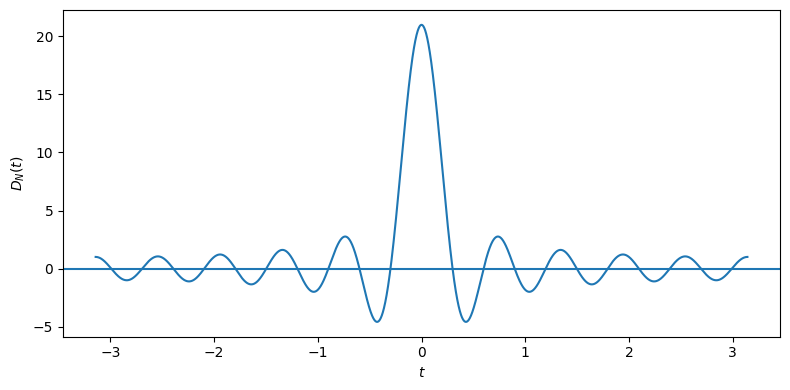
\includegraphics[width=0.6\textwidth]{nucleo-dirichlet.png}
  \caption{Núcleo de Dirichlet para $N=10$ y $L=2\pi$ (en la figura, sin el factor $1/L$).}
  \label{fig:nucleo-dirichlet}
\end{figure}
Para obtener una expresión más simple de $D_N(t)$, observemos que, si llamamos $r=e^{i\frac{2\pi}{L}t}$, entonces tenemos que
$$
L\,D_N(t) = \sum_{k=-N}^N r^k = \sum_{k=0}^{2N} r^{k-N} = r^{-N}\sum_{k=0}^{2N} r^k = r^{-N} \frac{1-r^{2N+1}}{1-r}.
$$
Ahora, multiplicando y dividiendo por $r^{-\frac12}$, obtenemos
$$
L\,D_N(t) = \frac{r^{-N-\frac12}}{r^{-\frac12}}\frac{1-r^{2N+1}}{1-r} = \frac{r^{-N-\frac12} - r^{N+\frac12}}{r^{-\frac12} - r^{\frac12}}.
$$
Reemplazando $r$ por $e^{i\frac{2\pi}{L}t}$, obtenemos
$$
D_N(t) = \frac{1}{L}\,\frac{e^{-i\frac{2\pi}{L}t (N+\frac12)} - e^{i\frac{2\pi}{L}t (N+\frac12)}}{e^{-i\frac{2\pi}{L}t\frac12} - e^{i\frac{2\pi}{L}t\frac12}} = \frac{1}{L}\,\frac{\sin(\frac{2\pi}{L}(N+\frac12)t)}{\sin(\frac{\pi}{L}t)}.
$$
El núcleo de Dirichlet tiene estas propiedades cuya demostración queda de ejercicio:
\begin{enumerate}
\item $D_N(t)$ es una función periódica de período $L$.

\item $D_N(t)$ es una función par.

\item $\int_{-L/2}^{L/2} D_N(t)\, dt = 1$ y, por paridad, $\int_{0}^{L/2} D_N(t)\, dt = \frac12$.
\end{enumerate}

Usando la propiedad 1 y el cambio de variables $s\mapsto t-s$,
$$
S_N[f](t) = \int_{-L/2}^{L/2} f(t-s)D_N(s)\, ds = \int_{0}^{L/2} \bigl(f(t-s)+f(t+s)\bigr)D_N(s)\, ds,
$$
donde en el último paso usamos la paridad de $D_N$ para juntar las contribuciones de $s$ y de $-s$. Entonces, usando la propiedad 3 obtenemos
\begin{align*}
S_N[f](t_0) - S &= \int_0^{L/2} \bigl(f(t_0-s) + f(t_0+s) - 2S\bigr) D_N(s)\, ds\\
& = \frac{1}{L} \int_0^{L/2} \frac{f(t_0+s)+f(t_0-s) - 2S}{s}\, \frac{s}{\sin(\frac{\pi}{L}s)}\,\sin\Bigl(\tfrac{2\pi}{L}\bigl(N+\tfrac12\bigr)s\Bigr)\, ds.
\end{align*}

Observemos que la función $s/\sin(\frac{\pi}{L}s)$ es continua y acotada en $[0,L/2]$ (vale $L/\pi$ en $s=0$ y $L/2$ en $s=L/2$; acá es esencial haber integrado sobre el intervalo simétrico $[-L/2,L/2]$ y no sobre $[0,L]$, donde el seno se anula en el extremo). Por otro lado, por la condición de Dini \eqref{Dini.cond}, la función $\phi(s) = \frac{f(t_0+s)+f(t_0-s) - 2S}{s}$ es integrable en $[0,\delta]$, y en $[\delta,L/2]$ es integrable porque $f\in L^1$ y $1/s\le 1/\delta$. Luego el producto $\phi(s)\, s/\sin(\frac{\pi}{L}s)$ es integrable en $[0,L/2]$ y podemos usar el Lema de Riemann--Lebesgue, Lema \ref{lema.RL} (con $\lambda = \frac{2\pi}{L}(N+\frac12)$, tomando la parte imaginaria), para concluir que $S_N[f](t_0) - S\to 0$ cuando $N\to\infty$. Esto concluye la demostración.
\end{proof}


Veamos ahora algunos ejemplos.

\begin{ejem}[Función signo]
La función signo se define como
$$
\operatorname{sg} t = \begin{cases}
1 & \text{si } t>0,\\
0 & \text{si } t=0,\\
-1 & \text{si } t<0.
\end{cases}
$$
Consideramos el intervalo $[-1, 1]$ y extendemos $\operatorname{sg} t$ por periodicidad a toda la recta real. Se puede ver el gráfico en la Figura \ref{fig:signo}.
\begin{figure}[ht]
  \centering
  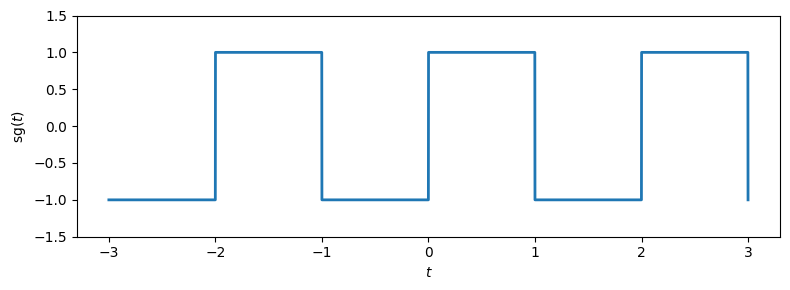
\includegraphics[width=0.7\textwidth]{signo.png}
  \caption{Función signo.}
  \label{fig:signo}
\end{figure}
De acuerdo a la Proposición \ref{prop.coef}, ítem 5, como $\operatorname{sg} t$ es real e impar, su serie de Fourier es una serie de senos. La serie de Fourier resulta:
$$
\operatorname{sg} t = \frac{4}{\pi}(\sin(\pi t) + \tfrac13\sin(3\pi t) + \tfrac15 \sin(5\pi t) +\cdots) = \frac{4}{\pi} \sum_{k=0}^\infty \frac{1}{2k+1} \sin((2k+1)\pi t).
$$
En la Figura \ref{fig:signo-aproximacion} se ven algunas aproximaciones de la función signo usando Fourier.
\begin{figure}[ht]
  \centering
  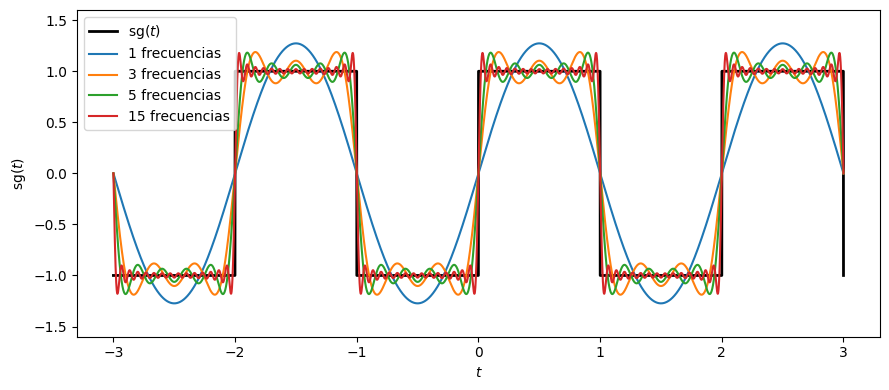
\includegraphics[width=0.7\textwidth]{signo-aproximacion.png}
  \caption{Función signo y algunas aproximaciones usando la serie de Fourier.}
  \label{fig:signo-aproximacion}
\end{figure}
Observemos que en $t=\frac12$ la función es diferenciable, por lo que podemos aplicar el Teorema \ref{teo.Dini} y entonces
$$
1 = \operatorname{sg}\tfrac12 = \frac{4}{\pi} \sum_{k=0}^\infty \frac{1}{2k+1} \sin((2k+1)\pi \tfrac12).
$$
Ahora, 
$$
\sin((2k+1)\pi \tfrac12) = \sin(\tfrac{\pi}{2} + k\pi) = (-1)^{k}. 
$$
Luego,
$$
\frac{\pi}{4} = \sum_{k=0}^\infty \frac{(-1)^k}{2k+1} = 1 - \frac13 + \frac15 - \frac17 + \cdots
$$
\end{ejem}

\begin{ejem}
Consideremos ahora la función $f(t)=t^2$. La suponemos definida en el intervalo $[-1, 1]$ y la extendemos por periodicidad a todo $\R$. Ver Figura \ref{fig:cuadratica}
\begin{figure}[ht]
  \centering
  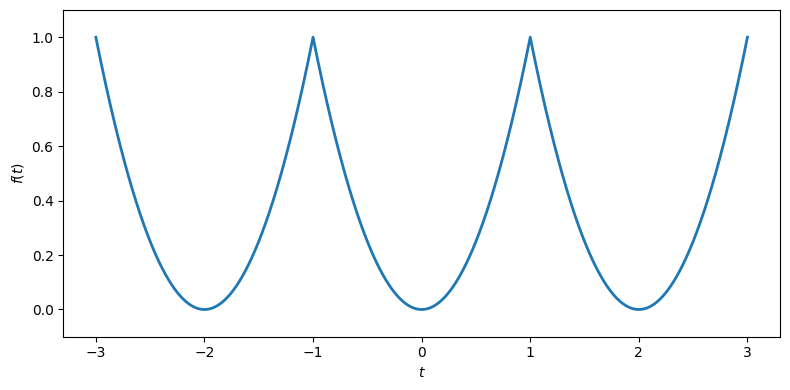
\includegraphics[width=0.7\textwidth]{cuadratica.png}
  \caption{$f(t)=t^2$ extendida por periodicidad.}
  \label{fig:cuadratica}
\end{figure}
De acuerdo a la Proposición \ref{prop.coef}, ítem 4, como $f(t)$ es real y par, su serie de Fourier es una serie de cosenos. La serie de Fourier resulta:
$$
t^2 = \frac13 + \frac{4}{\pi^2} \sum_{k=1}^\infty \frac{(-1)^k}{k^2}\cos(k\pi t),\quad t\in [-1, 1].
$$
En la Figura \ref{fig:cuadratica-aproximaciones} se muestran las aproximaciones que se obtienen mediante la serie de Fourier.
\begin{figure}[ht]
  \centering
  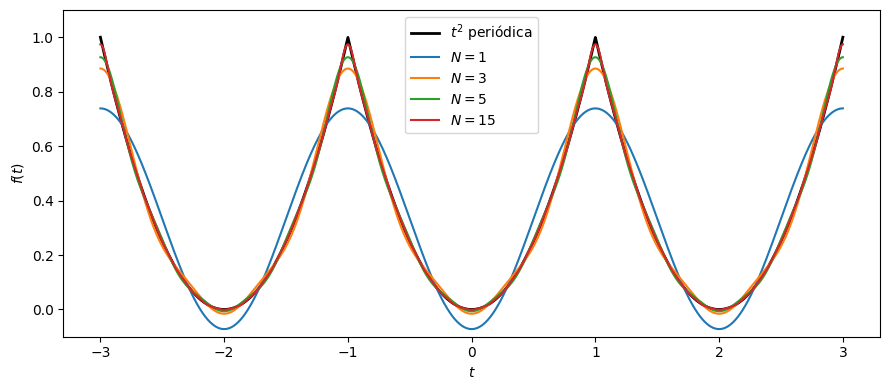
\includegraphics[width=0.7\textwidth]{cuadratica-aproximaciones.png}
  \caption{Aproximaciones de $f(t)=t^2$ mediante Fourier.}
  \label{fig:cuadratica-aproximaciones}
\end{figure}
Como $f(t)$ es diferenciable en $t=0$ podemos aplicar el Teorema \ref{teo.Dini} y obtenemos
$$
0 =  \frac13 + \frac{4}{\pi^2} \sum_{k=1}^\infty \frac{(-1)^k}{k^2}.
$$
Luego,
$$
\frac{\pi^2}{12} =  \sum_{k=1}^\infty \frac{(-1)^{k+1}}{k^2} = 1 - \frac14 + \frac19 - \frac{1}{16} + \cdots
$$
\end{ejem}

\section{Convergencia Uniforme}
Dada una señal $f\colon \R\to\C$, periódica con período $L$, recordemos que su serie de Fourier viene dada por
\begin{equation}\label{serie.f}
f(t)\sim \sum_{k=-\infty}^\infty c_k\, e^{i\frac{2k\pi}{L}t}.
\end{equation}
Esta serie está bien definida si $f$ es integrable.

En el capítulo previo, vimos condiciones que garantizan que la serie converge puntualmente (ver el Teorema \ref{teo.Dini}). Si $f$ resulta continua en $t_0$ y verifica la condición de Dini en $t_0$, \eqref{Dini.cond}, entonces
$$
f(t_0)= \sum_{k=-\infty}^\infty c_k\, e^{i\frac{2k\pi}{L}t_0}.
$$
En este capítulo queremos encontrar condiciones que garanticen que la serie converja uniformemente a $f$.

Para estudiar este problema, necesitaremos el siguiente resultado
\begin{teo}[Criterio $M$ de Weierstrass]\label{MdeW}
Sean $f_k\colon I\subset \R\to \C$, $k\in\N$ funciones y sean constantes $M_k>0$ tales que
$$
|f_k(t)|\le M_k\ \text{para todo } k\in\N\quad \text{y}\quad \sum_{k=1}^\infty M_k <\infty.
$$
Entonces, la serie $\sum_{k=1}^\infty f_k(t),$ converge absoluta y uniformemente en $I$.
\end{teo}

La demostración de este resultado la encuentran en \cite{Rudin}.

Usando el Teorema \ref{MdeW} tenemos el siguiente corolario:

\begin{cor}\label{cor.unif}
Sea $f\colon [0, L]\to\C$ una función integrable. Entonces la serie de Fourier de $f$ dada por \eqref{serie.f} converge absoluta y uniformemente si
\begin{equation}\label{ck.sumable}
\sum_{k=-\infty}^\infty |c_k| <\infty.
\end{equation}
\end{cor}

\begin{proof}
La serie de Fourier de $f$ es una serie de funciones donde $f_k(t) = c_k\, e^{i\frac{2k\pi}{L}t}$. Buscamos aplicar el Teorema \ref{MdeW}. Entonces
$$
|f_k(t)| = |c_k\, e^{i\frac{2k\pi}{L}t}| = |c_k|.
$$
Luego, tomando $M_k=|c_k|$ aplicamos el Teorema \ref{MdeW} y concluimos lo deseado.
\end{proof}

Veamos bajo qué condiciones sobre $f$ podemos garantizar que se cumple \eqref{ck.sumable}.

Observemos que por la Proposición \ref{prop.coef}, ítem 3, si $f$ es continua, diferenciable a trozos y $f'$ es integrable, tenemos que
$$
c_k(f) = \frac{L}{2k\pi i}\, c_k(f').
$$
Por otro lado, por el ítem 1 de la misma proposición, $|c_k(f')|$ es acotado, con lo que tenemos
$$
|c_k(f)|\le \frac{C}{k},\qquad C=\frac{1}{2\pi}\int_0^L |f'(t)|\, dt. 
$$

Si adicionalmente, suponemos que $f'$ es periódica de período $L$ y diferenciable con $f''$ integrable, aplicando nuevamente la Proposición \ref{prop.coef}, ítem 3, tenemos que
$$
c_k(f) = \frac{L}{2k\pi i} c_k(f') = \Bigr(\frac{L}{2k\pi i}\Bigr)^2c_k(f'') = -\frac{L^2}{4k^2\pi^2} c_k(f''),
$$
de donde, usando nuevamente el ítem 1 de la misma proposición,
\begin{equation}\label{ck.k2}
|c_k(f)|\le \frac{C}{k^2}.
\end{equation}
Luego tenemos el siguiente resultado.
\begin{prop}\label{prop.unif}
Sea $f\colon \R\to\C$ una función $L-$periódica, dos veces diferenciable con $f'$ $L-$periódica y $f''$ integrable en el $[0,L]$. Entonces la serie de Fourier de $f$ converge absoluta y uniformemente a $f$ en $[0,L]$.
\end{prop}

\begin{proof}
El resultado es una consecuencia inmediata del Corolario \ref{cor.unif} y la estimación \eqref{ck.k2}.
\end{proof}

Si bien este resultado ya nos da condiciones suficientes para la convergencia uniforme de la serie de Fourier, las mismas parecen excesivas. En lo que sigue veremos cómo es posible obtener la misma conclusión de la Proposición \ref{prop.unif} con menos hipótesis sobre la función $f$.

Observemos que, por el Lema de Riemann-Lebesgue, Lema \ref{lema.RL}, sabemos que $c_k(f')\to 0$ cuando $|k|\to\infty$. Por lo que 
$$
|c_k(f)| \le C \frac{1}{k} \underbrace{|c_k(f')|}_{\to 0}.
$$
Si bien esta estimación no alcanza para deducir que $c_k(f)$ satisface \eqref{ck.sumable}, no parece estar muy lejos. Es por esto que las hipótesis de la Proposición \ref{prop.unif} parecen excesivas.

Empecemos haciendo la siguiente observación. Sea $N\in\N$ y llamemos
\begin{equation}\label{pol.trig}
p_N(t) = \sum_{k=-N}^N d_k\, e^{i\frac{2k\pi}{L} t},\quad d_k\in\C.
\end{equation}
La ortogonalidad de las exponenciales complejas implican que
\begin{equation}\label{plancherel1}
\frac{1}{L}\int_0^L |p_N(t)|^2\, dx = \sum_{k=-N}^N |d_k|^2
\end{equation}
La igualdad \eqref{plancherel1} se denomina la {\em identidad de Plancherel} para polinomios trigonométricos.

Supondremos en lo que sigue que la función $f$ es de cuadrado integrable. Es decir que
$$
\frac{1}{L}\int_0^L |f(t)|^2\, dt < \infty.
$$
El conjunto de estas funciones se denota como $L^2([0,L])$.

Empecemos con el siguiente lema
\begin{lema}\label{mejor.aprox}
Sea $f$ una función $L-$periódica tal que $f\in L^2([0,L])$. Sea $N\in\N$ y llamemos $S_N[f]$ a la suma parcial de Fourier dada por 
$$
S_N[f](t) = \sum_{k=-N}^N c_k\, e^{i\frac{2k\pi}{L} t},
$$
con $c_k\in\C$ los coeficientes de Fourier dados por \eqref{coef.fourier}. Entonces si $p_N(t)$ es un polinomio trigonométrico de la forma \eqref{pol.trig}, tenemos que
$$
\frac{1}{L}\int_0^L |f(t)-S_N[f](t)|^2\, dt \le \frac{1}{L}\int_0^L |f(t)-p_N(t)|^2\, dt.
$$
\end{lema}

\begin{obs}
Lo que el Lema está diciendo es que entre todos los polinomios trigonométricos, el que mejor aproxima a la función $f$ en {\em media cuadrática} es la aproximación de Fourier.
\end{obs}

\begin{proof}
Sea $p_N(t)$ dado por \eqref{pol.trig}. Empecemos calculando 
$$
\int_0^L |f(t)-p_N(t)|^2\, dt = \int_0^L |f(t)|^2\, dt - 2\Re\left(\int_0^L f(t)\overline{p_N(t)}\, dt\right) + \int_0^L |p_N(t)|^2\, dt.
$$
Ahora, por \eqref{coef.fourier},
$$
\int_0^L f(t)\overline{p_N(t)}\, dt = \sum_{k=-N}^N \bar d_k \underbrace{\int_0^L f(t)\, e^{-i\frac{2k\pi}{L}t}\, dt}_{L c_k}
$$
Usando \eqref{plancherel1}, 
$$
\int_0^L |p_N(t)|^2\, dt = L \sum_{k=-N}^N |d_k|^2.
$$
Luego, obtenemos
$$
\int_0^L |f(t)-p_N(t)|^2\, dt = \int_0^L |f(t)|^2\, dt - 2L\Re\left(\sum_{k=-N}^N c_k \bar d_k\right) + L \sum_{k=-N}^N |d_k|^2.
$$
Sumando y restando $L\sum_{k=-N}^N |c_k|^2$, llegamos a
\begin{equation}\label{cotack}
\int_0^L |f(t)-p_N(t)|^2\, dt = \int_0^L |f(t)|^2\, dt - L\sum_{k=-N}^N |c_k|^2 + L\sum_{k=-N}^N |c_k-d_k|^2.
\end{equation}
El lema queda demostrado obervando que esta última expresión se minimiza si $d_k=c_k$ para todo $k$
\end{proof}

Un corolario inmediato del lema (en realidad de \eqref{cotack}) es la llamada {\em desigualdad de Bessel}.
\begin{cor}[Desigualdad de Bessel]
Sea $f\in L^2([0,L])$ y $c_k$ sus coeficientes de Fourier dados por \eqref{coef.fourier}. Entonces
\begin{equation}\label{Bessel}
\sum_{k=-\infty}^\infty |c_k|^2\le \frac{1}{L}\int_0^L |f(t)|^2\, dt.
\end{equation}
\end{cor}

\begin{proof}
Si en \eqref{cotack} tomamos $d_k=c_k$, obtenemos
$$
0\le \int_0^L |f(t)-S_N(t)|^2\, dt = \int_0^L |f(t)|^2\, dt - L\sum_{k=-N}^N |c_k|^2.
$$
Luego,
$$
\sum_{k=-N}^N |c_k|^2\le \frac{1}{L}\int_0^L |f(t)|^2\, dt, \quad \forall N\in\N,
$$
de donde se deduce lo deseado.
\end{proof}

Con la ayuda de la desigualdad de Bessel podemos ahora si dar un resultado de convergencia uniforme con mejores hipótesis que las de la Proposición \ref{prop.unif}.
\begin{teo}\label{teo.unif}
Sea $f$ una función $L-$periódica y diferenciable tal que $f'\in L^2([0,L])$. Entonces la serie de Fourier de $f$ converge absoluta y uniformemente a $f$ en $[0, L]$.
\end{teo}

\begin{proof}
De acuerdo al Corolario \ref{cor.unif}, sólo debemos verificar \eqref{ck.sumable}. Como $f$ es $L-$periódica y diferenciable, tenemos que
$$
|c_k(f)| = \frac{L}{2k\pi}|c_k(f')|.
$$
luego, usando la desigualdad $ab\le \frac{a^2}{2}+\frac{b^2}{2}$,
$$
|c_k(f)|\le \frac{L^2}{4\pi^2} \frac{1}{k^2} + \frac12 |c_k(f')|^2.
$$
Esta desigualdad, junto con la desigualdad de Bessel aplicada a los coeficientes $c_k(f')$, implican que $c_k(f)$ verifica \eqref{ck.sumable} y por ende la serie de Fourier es absoluta y uniformemente convergente.
\end{proof}

\section{Convergencia en media cuadrática}

El objetivo en esta sección es el de estudiar la convergencia de la serie de Fourier pero sin asumir hipótesis de regularidad sobre la función $f(t)$. Entonces no queremos asumir ni las hipótesis del Teorema \ref{teo.Dini} que nos da la convergencia puntual, y mucho menos las del Teorema \ref{teo.unif} que nos da la convergencia uniforme.

Queremos remarcar que, aunque asumamos que $f$ es una función continua, es posible construir ejemplos en donde $f$ es continua y su serie de Fourier no converge en un conjunto denso de puntos (ver \cite{Zygmund2}). Luego para estudiar estos casos en general, e incluso casos en donde $f$ es discontinua, precisamos ver una noción de convergencia diferente a la puntual. 

La noción adecuada resulta ser la convergencia en {\em media cuadrática} que ya hemos visto en el Lema \ref{mejor.aprox}.
\begin{defi}[Convergencia en media cuadrática]
Sean $f_k, f\in L^2([0,L])$, $k\in\N$. Decimos que $f_k\to f$ en $L^2$ o en media cuadrática si
$$
\int_0^L |f(t)-f_k(t)|^2\, dt \to 0 \quad \text{ cuando } k\to\infty.
$$
\end{defi}


Tenemos entonces el siguiente resultado.
\begin{teo}\label{teo.L2}
Sea $f\in L^2([0,L])$. Entonces su serie de Fourier converge en media cuadrática. Es decir,
$$
\int_0^L |f(t) - S_N[f](t)|^2\, dt \to 0 \quad \text{cuando } N\to\infty.
$$
\end{teo}

La demostración de este resultado usa dos hechos fundamentales. El primero es que las funciones $C^1_c([0,L])$ son densas en $L^2([0,L])$:
\begin{teo}\label{densoL2}
Sea $f\in L^2([0,L])$ y $\ve>0$. Entonces existe $f_\ve\in C^1_c([0,L])$ tal que
$$
\int_0^L |f(t)-f_\ve(t)|^2\, dt < \ve.
$$
\end{teo}

Este resultado lo pueden encontrar en \cite{Zygmund}.

El segundo resultado que vamos a necesitar es el Teorema de Stone-Weierstrass:
\begin{teo}[Stone-Weierstrass]\label{teo.SW}
El conjunto de los polinomios trigonométricos de período $L$ es denso en el espacio $C_{per}([0,L])$ de las funciones continuas en $[0,L]$ con $g(0)=g(L)$ (es decir, las funciones continuas y $L$-periódicas). Es decir, dado $g\in C_{per}([0,L])$ y $\ve>0$ existe un polinomio trigonométrico $p_\ve$ tal que
$$
\sup_{t\in [0,L]} |g(t)-p_\ve(t)| < \ve.
$$
\end{teo}

Este teorema se encuentra en \cite{Rudin}.

\begin{obs}
La condición $g(0)=g(L)$ es necesaria: los polinomios trigonométricos son periódicos, y el límite uniforme de funciones periódicas es periódico. Notemos que las funciones de $C^1_c([0,L])$ del Teorema \ref{densoL2} se anulan en los extremos y por lo tanto pertenecen a $C_{per}([0,L])$, que es lo que se usa en la demostración de abajo. El Teorema de Stone-Weierstrass es en realidad más general que el que enunciamos acá. Esta versión es la que vamos a usar pero el lector interesado puede ver en \cite{Rudin} la versión general del mismo.
\end{obs}

Ahora sí, veamos la demostración.
\begin{proof}[Demostración del Teorema \ref{teo.L2}]
Sea $f\in L^2([0,L])$ y $\ve>0$. Por el Teorema \ref{densoL2}, existe $f_\ve\in C^1_c([0,L])$ tal que 
$$
\left(\int_0^L |f(t)-f_\ve(t)|^2\, dt\right)^\frac12 < \frac{\ve}{2}.
$$
Ahora, por el Teorema \ref{teo.SW}, existe un polinomio trigonométrico $p_\ve$ tal que
$$
\sup_{t\in [0,L]} |f_\ve(t)-p_\ve(t)| < \frac{\ve}{2\sqrt{L}}.
$$
El polinomio $p_\ve$ es de la forma
$$
p_\ve(t) = \sum_{k=-N}^N d_k^\ve\, e^{i\frac{2k\pi}{L}t}
$$
y por el Lema \ref{mejor.aprox} tenemos que
$$
\int_0^L |f(t)-S_N[f](t)|^2\, dt \le \int_0^L |f(t) - p_\ve(t)|^2\, dt.
$$
Luego, combinamos todas estas desigualdades y obtenemos
\begin{align*}
\left(\int_0^L |f(t)-S_N[f](t)|^2\, dt\right)^\frac12 &\le \left(\int_0^L |f(t) - p_\ve(t)|^2\, dt\right)^\frac12\\
& \le \left(\int_0^L |f(t) - f_\ve(t)|^2\, dt\right)^\frac12 + \left(\int_0^L |f_\ve(t) - p_\ve(t)|^2\, dt\right)^\frac12\\
&\le \frac{\ve}{2} + \sqrt{L}  \sup_{t\in [0,L]} |f_\ve(t)-p_\ve(t)|\\
& \le \frac{\ve}{2} + \frac{\ve}{2} = \ve,
\end{align*}
lo que completa la demostración.
\end{proof}

Con la ayuda del Teorema \ref{teo.L2} podemos demostrar la famosa {\em identidad de Plancherel}
\begin{cor}[Identidad de Plancherel]\label{plancherel}
Sea $f\in L^2([0,L])$ y $c_k$ sus coeficientes de Fourier dados por \eqref{coef.fourier}. Entonces
$$
\frac{1}{L}\int_0^L |f(t)|^2\, dt = \sum_{k=-\infty}^\infty |c_k|^2.
$$
\end{cor}

\begin{proof}
La demostración es inmediata de los siguiente hechos: Llamemos
$$
S_N[f](t) = \sum_{k=-N}^N c_k\, e^{i \frac{2k\pi}{L}t}.
$$
Entonces
\begin{align*}
\text{(a)}\ &\frac{1}{L}\int_0^L |S_N[f](t)|^2\, dt = \sum_{k=-N}^N |c_k|^2 \quad \text{y}\\
\text{(b)}\ &\int_0^L |f(t) - S_N[f](t)|^2\, dt \to 0, \quad \text{cuando } N\to\infty.
\end{align*}
Los detalles quedan para el lector.
\end{proof}

\section{El fenómeno de Gibbs}

Uno de los aspectos más llamativos —y a primera vista paradójicos— de la convergencia de las series de Fourier es el llamado \emph{fenómeno de Gibbs}. Este fenómeno describe el comportamiento de las sumas parciales de la serie de Fourier cerca de un punto de discontinuidad de la función original.

Sea $f$ una función $L-$periódica y consideremos su serie de Fourier. Aun cuando la serie converge puntualmente en todos los puntos donde $f$ es continua y converge al valor medio de los límites laterales en los puntos de discontinuidad, las sumas parciales
$$
S_N[f](t) = \sum_{k=-N}^N c_k\, e^{i \frac{2k\pi}{L} t}
$$
presentan oscilaciones persistentes cerca de las discontinuidades.

Más precisamente, si $f$ tiene un salto en un punto $t_0$, las sumas parciales exhiben un sobrepico (overshoot) y un subpico (undershoot) cerca de $t_0$, cuya amplitud no desaparece cuando $N \to \infty$. En particular, el máximo exceso relativo converge a una constante universal, aproximadamente un $9\%$ del tamaño del salto, independientemente de la función considerada.

Este comportamiento no contradice los teoremas clásicos de convergencia puntual, como el Teorema de Dini, Teorema \ref{teo.Dini}, ya que dichos resultados garantizan convergencia punto a punto, pero no convergencia uniforme en presencia de discontinuidades.

Desde un punto de vista analítico, el fenómeno de Gibbs está íntimamente ligado a la forma del núcleo de Dirichlet,
$$
D_N(t) = \frac{1}{L}\sum_{k=-N}^N e^{i \frac{2k\pi}{L} t},
$$
cuyas oscilaciones y pobre comportamiento integrable explican la aparición de estos efectos cerca de los saltos de la función.

\subsection{Ejemplos ilustrativos}

El ejemplo prototípico del fenómeno de Gibbs es la función signo
$$
f(t) = \operatorname{sg}(t), \qquad t \in (-1,1),
$$
extendida por periodicidad. En este caso, las sumas parciales de su serie de Fourier muestran oscilaciones pronunciadas cerca de $t=0$ y en los puntos $\pm 1$, que no desaparecen al aumentar el número de términos, aunque se concentran en regiones cada vez más pequeñas. En la Figura \ref{fig:signo-aproximacion} vimos como la serie de Fourier aproxima a la función pero presenta oscilaciones cerca de las discontinuidades. ¿Qué sucede si aumentamos el grado de aproximación?
\begin{figure}[ht]
  \centering
  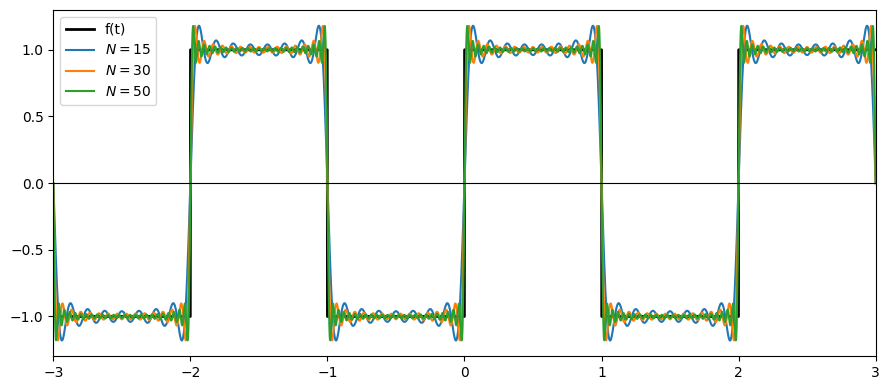
\includegraphics[width=0.7\textwidth]{signo-aproximacion2.png}
  \caption{Fenómeno de Gibbs para la función signo.}
  \label{fig:signo-aproximacion2}
\end{figure}
Como se observa en la Figura \ref{fig:signo-aproximacion2} la oscilación no disminuye al aumentar el grado de aproximación. En la Figura \ref{fig:signo-detalle} se observa el detalle sobre la singularidad y como el error se mantiene constante.
\begin{figure}[ht]
  \centering
  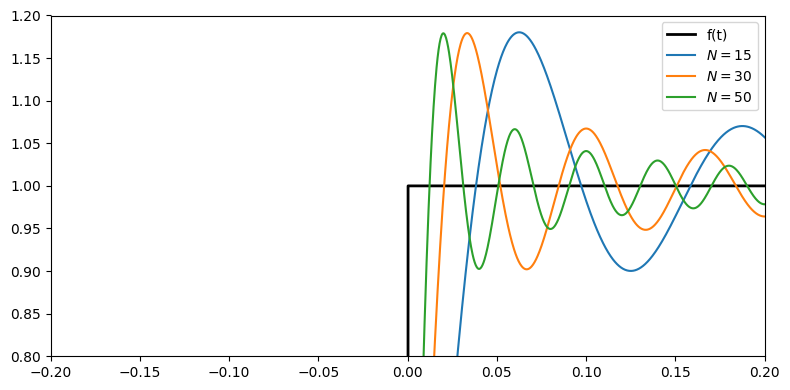
\includegraphics[width=0.7\textwidth]{signo-detalle.png}
  \caption{Detalle del fenómeno de Gibbs para la función signo.}
  \label{fig:signo-detalle}
\end{figure}
Observemos que aunque el error absoluto se mantiene constante, el tamaño de la región en donde el error es cometido disminuye a medida que aumentamos el grado de aproximación.

Otro ejemplo clásico es la función diente de sierra
$$
f(t) = t, \qquad t \in (-1,1),
$$
extendida periódicamente (ver Figura \ref{fig:diente}). A pesar de ser continua, la función presenta discontinuidades en los extremos del intervalo fundamental, y el fenómeno de Gibbs se manifiesta nuevamente cerca de esos puntos. Ver Figura \ref{fig:diente-gibbs}
\begin{figure}[ht]
  \centering
  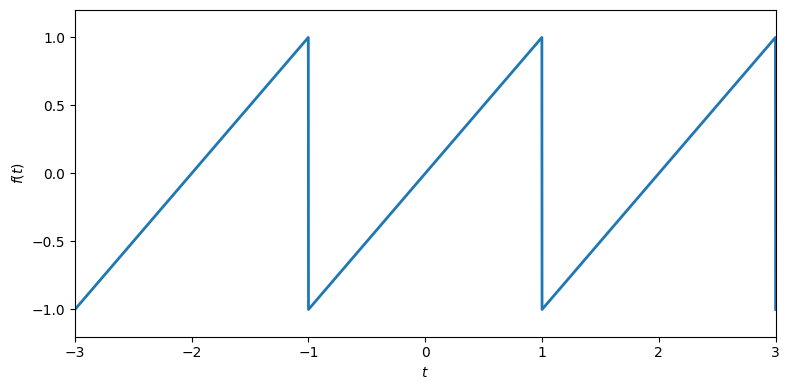
\includegraphics[width=0.6\textwidth]{diente.png}
  \caption{Función diente de sierra.}
  \label{fig:diente}
\end{figure}
\begin{figure}[ht]
  \centering
  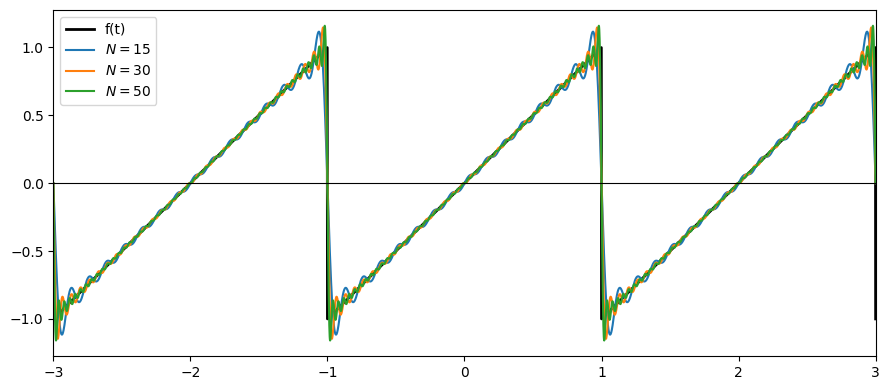
\includegraphics[width=0.7\textwidth]{diente-gibbs.png}
  \caption{Fenómeno de Gibbs para la función diente de sierra.}
  \label{fig:diente-gibbs}
\end{figure}
Nuevamente si vemos el detalle de este gráfico se observa que si bien el error absoluto no disminuye a medida que se aumenta el grado de aproximación, si disminuye el tamaño de la región en donde ese error es grande. Ver Figura \ref{fig:diente-detalle}
\begin{figure}[ht]
  \centering
  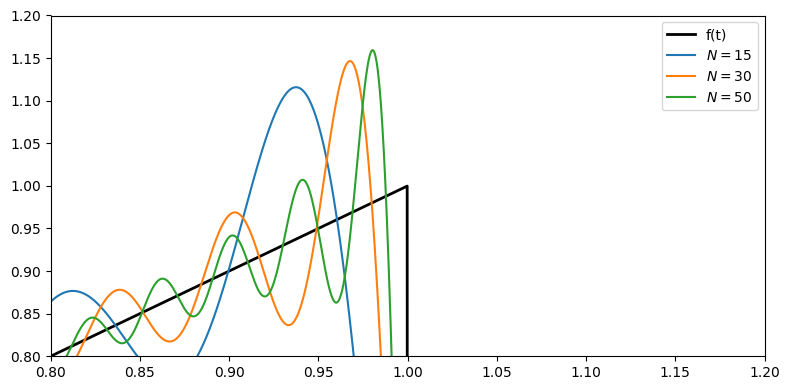
\includegraphics[width=0.7\textwidth]{diente-detalle.png}
  \caption{Detalle del fenómeno de Gibbs para la función diente de sierra.}
  \label{fig:diente-detalle}
\end{figure}

Estos ejemplos muestran que el fenómeno de Gibbs no es una patología excepcional, sino una característica estructural de la aproximación por series de Fourier de funciones con falta de regularidad, y pone de manifiesto las limitaciones de las aproximaciones espectrales basadas en truncaciones finitas.



\chapter{Transformada de Fourier}

La transformada de Fourier surge como una extensión natural de las series de Fourier al estudio de señales no periódicas. Mientras que las series de Fourier permiten descomponer funciones periódicas como superposiciones discretas de ondas armónicas, muchas señales de interés en aplicaciones reales —mediciones experimentales, señales temporales finitas, datos observados en ventanas de tiempo acotadas— no presentan periodicidad. La transformada de Fourier proporciona entonces un marco continuo que permite analizar el contenido frecuencial de este tipo de señales.

Históricamente, la transformada de Fourier aparece a fines del siglo XIX como un límite formal de las series de Fourier cuando el período tiende a infinito. Este pasaje, inicialmente heurístico, fue posteriormente formalizado en distintos contextos funcionales a lo largo del desarrollo del análisis moderno. A lo largo del siglo XX, la transformada de Fourier se consolidó como una herramienta central en matemática aplicada, física matemática, teoría de señales y procesamiento de información, con un rol fundamental en el estudio de ecuaciones en derivadas parciales, óptica, mecánica cuántica y teoría de comunicaciones.

Desde el punto de vista conceptual, la transformada de Fourier permite reinterpretar una señal como una superposición continua de ondas planas de distintas frecuencias. Esta representación dual —en el dominio del tiempo o del espacio, y en el dominio de las frecuencias— resulta particularmente poderosa para el análisis de estructuras ocultas en los datos, la identificación de escalas relevantes y la separación de fenómenos de distinta naturaleza.

En el contexto de la Ciencia de Datos, la transformada de Fourier ocupa un lugar central en numerosas aplicaciones. Entre ellas se destacan el procesamiento y filtrado de señales, la eliminación de ruido (\emph{denoising}), el análisis espectral de series temporales, la detección de patrones periódicos, la compresión de información y la resolución eficiente de problemas inversos. Incluso cuando los datos son discretos y finitos, las ideas subyacentes a la transformada de Fourier continúan siendo fundamentales y motivan algoritmos computacionales ampliamente utilizados, como la transformada discreta de Fourier y la FFT.

En este capítulo introduciremos la transformada de Fourier desde un punto de vista principalmente aplicado, poniendo énfasis en su interpretación, sus propiedades fundamentales y su relación con las series de Fourier estudiadas previamente. 

\section{De las series de Fourier a la transformada de Fourier}

En el capítulo anterior estudiamos la representación de funciones periódicas mediante series de Fourier, es decir, como superposiciones discretas de ondas armónicas cuyas frecuencias están cuantizadas por el período de la función. Sin embargo, muchas señales de interés en aplicaciones no son periódicas, o bien pueden pensarse como observaciones realizadas en intervalos de tiempo muy grandes en comparación con las escalas características del fenómeno. Esto motiva la búsqueda de una representación análoga que permita tratar funciones definidas en todo $\R$ sin imponer periodicidad.

Una forma natural de abordar este problema consiste en considerar una función $f$ definida en un intervalo $(-L/2,L/2)$ y extenderla periódicamente. Su serie de Fourier puede escribirse, en forma compleja, como
$$
f_L(t) \sim \sum_{k\in\Z} c_k^{(L)}\, e^{i \frac{2\pi k}{L} t}, \qquad c_k^{(L)} = \frac{1}{L} \int_{-L/2}^{L/2} f(t)\, e^{-i \frac{2\pi k}{L} t}\, dt.
$$

A medida que el período $L$ aumenta, el espaciamiento entre las frecuencias
$$
\xi_k = \frac{k}{L}
$$
se hace cada vez más pequeño. En el límite formal $L\to\infty$, el conjunto discreto de frecuencias se aproxima a un continuo, y la suma sobre $k$ puede interpretarse heurísticamente como una integral sobre la variable de frecuencia.

Más precisamente, si escribimos
$$
\sum_{k\in\Z} c_k^{(L)}\, e^{2\pi i \xi_k t} \;\approx\; \sum_k \hat f(\xi_k)\, e^{2\pi i \xi_k t}\,\Delta \xi, \qquad \Delta \xi = \frac{1}{L},
$$
entonces, al hacer $L\to\infty$, esta suma de Riemann conduce formalmente a una representación integral de la forma
$$
f(t) = \int_{-\infty}^{\infty} \hat f(\xi)\, e^{2\pi i \xi t}\, d\xi,
$$
donde la función $\hat f(\xi)$ describe la contribución de cada frecuencia $\xi$ a la señal original.

Este razonamiento heurístico conduce a la definición de la transformada de Fourier
\begin{equation}\label{fourier.trans}
\hat f(\xi) = \int_{-\infty}^{\infty} f(t)\, e^{-2\pi i\xi t}\, dt,
\end{equation}
junto con su fórmula de inversión
\begin{equation}\label{fourier.inverse}
f(t) = \int_{-\infty}^{\infty} \hat f(\xi)\, e^{2\pi i\xi t}\, d\xi,
\end{equation}
que será estudiada con mayor detalle en las secciones siguientes.

Desde este punto de vista, la transformada de Fourier puede entenderse como el análogo continuo de las series de Fourier: mientras que las series describen funciones periódicas como superposiciones discretas de ondas armónicas, la transformada de Fourier describe funciones no periódicas como superposiciones continuas de ondas planas. Esta transición del régimen discreto al continuo es central tanto en el desarrollo teórico del análisis armónico como en sus aplicaciones modernas al procesamiento de señales y al análisis de datos.

\subsection{Convenciones y normalizaciones}

En el capítulo anterior estudiamos la descomposición de funciones periódicas en series de Fourier. Allí, el carácter periódico del problema conduce de manera natural a un espectro \emph{discreto} de frecuencias, indexado por enteros. Cuando se abandona la hipótesis de periodicidad y se consideran funciones definidas en todo $\R$, este espectro se vuelve \emph{continuo}, y la suma discreta es reemplazada por una integral. Este pasaje conduce a la \emph{transformada de Fourier}.

A diferencia de las series de Fourier, la transformada no posee una definición única universalmente adoptada. Existen varias \emph{convenciones}, todas matemáticamente equivalentes entre sí, que difieren únicamente en la ubicación de factores constantes (en particular potencias de $2\pi$) y en la elección del signo en los exponentes complejos. Estas diferencias no afectan el contenido esencial de la teoría, pero sí modifican la forma explícita de muchas fórmulas.

Una convención muy utilizada, especialmente en análisis armónico y en aplicaciones modernas, define la transformada de Fourier de una función integrable $f:\R\to\C$ como
$$
\hat f(\xi) = \int_{\R} f(x)\, e^{-i \xi x}\, dx,
$$
con fórmula inversa
$$
f(x) = \frac{1}{2\pi}\int_{\R} \hat f(\xi)\, e^{i \xi x}\, d\xi.
$$
La elección que hicimos en \eqref{fourier.trans} tiene la ventaja de presentar una forma completamente simétrica entre la transformada directa y la inversa \eqref{fourier.inverse}, y de conectar de manera transparente con el límite de las series de Fourier cuando el período tiende a infinito.

Otras convenciones, frecuentes en física e ingeniería, distribuyen los factores $2\pi$ de manera distinta, por ejemplo colocándolos únicamente en la transformada inversa, o repartiéndolos de forma simétrica entre ambas. En todos los casos, las distintas definiciones se obtienen unas de otras mediante simples cambios de escala en la variable de frecuencia.

Es importante destacar que la elección de una convención fija determina la forma precisa de identidades fundamentales, como las fórmulas de derivación, convolución y las identidades de Parseval y Plancherel. Por esta razón, a lo largo de este texto adoptaremos una única convención y la mantendremos de manera consistente en todas las aplicaciones.

\section{Definición y propiedades fundamentales}

En esta sección introducimos la definición formal de la transformada de Fourier y estudiamos sus propiedades fundamentales. Estas se agrupan en propiedades algebraicas y propiedades analíticas, que explican el comportamiento estructural y regular de la transformada.


\begin{defi}
Sea $f\in L^1(\R)$. Definimos la \emph{transformada de Fourier} de $f$ como
\[
\hat f(\xi)=\int_{\R} f(x)\,e^{-2\pi i \xi x}\,dx,
\qquad \xi\in\R.
\]
\end{defi}

\begin{obs}
Esta integral está bien definida y satisface
\[
|\hat f(\xi)|\le \|f\|_{L^1(\R)}.
\]
\end{obs}

Veamos algunas de las propiedades fundamentales de la transformada.

\begin{prop}[Propiedades algebraicas]\label{prop.algebraica}
Sea $f\in L^1(\R)$. Entonces se cumplen las siguientes propiedades:
\begin{enumerate}
\item \textbf{Linealidad.}  
Si $\alpha,\beta\in\C$ y $f,g\in L^1(\R)$,
\[
\widehat{\alpha f+\beta g}=\alpha\hat f+\beta\hat g.
\]

\item \textbf{Conjugación.}  
Si $\bar{f}$ denota el conjugado complejo de $f$, entonces
\[
\widehat{\bar{f}}(\xi)=\overline{\hat f(-\xi)}.
\]

\item \textbf{Traslación.}  
Si $x_0\in\R$ y $g(x)=f(x-x_0)$, entonces
\[
\hat g(\xi)=e^{-2\pi i \xi x_0}\hat f(\xi).
\]

\item \textbf{Modulación.}  
Si $\xi_0\in\R$ y $g(x)=e^{2\pi i \xi_0 x}f(x)$, entonces
\[
\hat g(\xi)=\hat f(\xi-\xi_0).
\]

\item \textbf{Dilatación.}  
Si $a\neq 0$ y $g(x)=f(ax)$, entonces
\[
\hat g(\xi)=\frac{1}{|a|}\hat f\Bigr(\frac{\xi}{a}\Bigr).
\]
\end{enumerate}
\end{prop}

\begin{proof}
Todas las propiedades se verifican mediante cálculos directos usando la definición de la transformada y cambios de variables apropiados en la integral. A modo de ejemplo veamos la demostración de 5.

En efecto, si $g(x)=f(ax)$ con $a\neq 0$, tenemos
$$
\hat g(\xi) = \int_{-\infty}^\infty g(x)\, e^{-2\pi i \xi x}\, dx = \int_{-\infty}^\infty f(ax)\, e^{-2\pi i \xi x}\, dx.
$$
Realizamos entonces el cambio de variables $\bar x = ax$ con lo cual $d\bar x = |a|dx$ y llegamos a
$$
\hat g(\xi) = \int_{-\infty}^\infty f(\bar x)\, e^{-2\pi i \xi \frac{\bar x}{a}} \frac{1}{|a|}\, d\bar x = \frac{1}{|a|}\int_{-\infty}^\infty f(\bar x)\, e^{-2\pi i \frac{\xi}{a} \bar x}\, d\bar x = \frac{1}{|a|} \hat f\Bigr(\frac{\xi}{a}\Bigr).
$$
\end{proof}

\begin{obs}\label{rescale}
Observemos que, usando 1 y 5 de la proposición anterior obtenemos que si $\lambda>0$ y $g(x)=\frac{1}{\lambda} f(\frac{x}{\lambda})$, entonces
$$
\hat g(\xi) = \hat f(\lambda\xi).
$$
En efecto,
$$
\hat g(\xi) = \frac{1}{\lambda} \widehat{f(\lambda^{-1}x)}(\xi) = \frac{1}{\lambda} \frac{1}{\lambda^{-1}}\hat f\Bigr(\frac{\xi}{\lambda^{-1}}\Bigr) = \hat f(\lambda \xi).
$$
\end{obs}

Lo que sigue son algunas propiedades analíticas de la transformada de Fourier y son las propiedades que hacen que la transformada sea de extrema utilidad en el análisis.

\begin{prop}[Propiedades analíticas]\label{prop.analiticas}
Sea $f\in L^1(\R)$. Entonces:
\begin{enumerate}
\item \textbf{Continuidad uniforme.}  
La función $\hat f$ es uniformemente continua en $\R$.

\item \textbf{Derivación en el dominio físico.}  
Si $f$ es continuamente derivable y $f,f'\in L^1(\R)$, entonces
\[
\widehat{f'}(\xi)=2\pi i \xi\,\hat f(\xi).
\]

\item \textbf{Derivación en el dominio frecuencial.}  
Si $f$ y $x f(x)$ pertenecen a $L^1(\R)$, entonces $\hat f$ es derivable y
\[
(\hat f)'(\xi)=\widehat{-2\pi i x f(x)}(\xi).
\]

\item \textbf{Lema de Riemann--Lebesgue.}  
Se tiene
\[
\lim_{|\xi|\to\infty}\hat f(\xi)=0.
\]

\item \textbf{Identidad de dualidad.}  
Si $f,g\in L^1(\R)$, entonces
\[
\int_{\R}\hat f(\xi)\,g(\xi)\,d\xi
=
\int_{\R} f(x)\,\hat g(x)\,dx.
\]
\end{enumerate}
\end{prop}

\begin{proof}
\begin{enumerate}
\item Debemos verificar que $\hat f(\xi)\to \hat f(\xi_0)$ cuando $\xi\to\xi_0$. Esto es, hay que calcular el límite
$$
\lim_{\xi\to\xi_0} \int_{-\infty}^\infty f(x)\, e^{-2\pi i \xi x}\, dx.
$$
Para eso usaremos el Teorema de la convergencia dominada y necesitamos mayorar la expresión $\phi_\xi(x) = f(x)\, e^{-2\pi i \xi x}$ por una función integrable independiente de $\xi$. Pero
$$
|\phi_\xi(x)| = |f(x)|\in L^1(\R),
$$
de donde se concluye el resultado.

\item Integrando por partes,
$$
\widehat{f'}(\xi)=\int_{\R} f'(x)e^{-2\pi i \xi x}\,dx =2\pi i \xi\hat f(\xi),
$$
ya que el término de borde se anula por la integrabilidad de $f$.

\item Usando nuevamente el Teorema de la convergencia dominada de manera completamente análoga al punto 1, podemos derivar bajo el signo integral, obteniendo
$$
(\hat f)'(\xi)=\int_{\R} (-2\pi i x)f(x)e^{-2\pi i \xi x}\,dx = \widehat{-2\pi i x f(x)}(\xi).
$$

\item Recordemos primero que el espacio $C_c^1(\R)$ de funciones continuamente derivables con soporte compacto es denso en $L^1(\R)$.

Sea $\ve>0$. Por densidad, existe $g\in C_c^1(\R)$ tal que
\[
\|f-g\|_{L^1(\R)}<\ve.
\]
Escribimos
\[
\hat f(\xi)=\hat g(\xi)+\widehat{(f-g)}(\xi).
\]

Para el segundo término, se tiene
\[
|\widehat{(f-g)}(\xi)|
\le
\int_{\R} |f(x)-g(x)|\,dx
=
\|f-g\|_{L^1(\R)}
<
\ve,
\]
para todo $\xi\in\R$.

Resta estudiar el comportamiento de $\hat g(\xi)$ cuando $|\xi|\to\infty$.
Como $g\in C_c^1(\R)$, existe $R>0$ tal que $\operatorname{supp} g\subset[-R,R]$ y podemos integrar por partes:
\[
\hat g(\xi)
=
\int_{-R}^R g(x)\,e^{-2\pi i\xi x}\,dx
=
\frac{1}{-2\pi i\xi}\int_{-R}^R g(x)\,\frac{d}{dx}\bigl(e^{-2\pi i\xi x}\bigr)\,dx.
\]
Integrando por partes y usando que $g$ se anula en los extremos del intervalo, obtenemos
\[
\hat g(\xi)
=
\frac{1}{2\pi i\xi}\int_{-R}^R g'(x)\,e^{-2\pi i\xi x}\,dx.
\]
En consecuencia,
\[
|\hat g(\xi)|
\le
\frac{1}{2\pi |\xi|}\int_{-R}^R |g'(x)|\,dx
=
\frac{\|g'\|_{L^1(\R)}}{2\pi |\xi|},
\]
lo que implica que
\[
\lim_{|\xi|\to\infty} \hat g(\xi)=0.
\]

Combinando ambas estimaciones, existe $\xi_0$ tal que para $|\xi|>\xi_0$ se cumple
\[
|\hat f(\xi)|
\le
|\hat g(\xi)| + |\widehat{(f-g)}(\xi)|
<
\ve + \ve
=
2\ve.
\]
Como $\ve>0$ es arbitrario, se concluye que
\[
\lim_{|\xi|\to\infty} \hat f(\xi)=0.
\]

\item Se obtiene aplicando Fubini y reordenando las integrales.
\end{enumerate}
\end{proof}

Veamos finalmente algunos ejemplos. Los primeros se obtienen mediante el cálculo directo de las integrales.

\begin{ejem}[Función característica de un intervalo]\label{ej:indicadora}
Sea $f=\mathbf{1}_{[-1,1]}$. Entonces
\[
\hat f(\xi)=\int_{-1}^{1}e^{-2\pi i \xi x}\,dx
=\frac{\sin(2\pi\xi)}{\pi\xi}.
\]
\end{ejem}

Para este segundo ejemplo, es conveniente demostrar primero la fórmula
$$
\int_0^\infty e^{-ax}\cos(bx)\, dx = \frac{a}{a^2+b^2},\quad a>0.
$$
La demostración de esta fórmula se obtiene mediante la aplicación de la fórmula de integración por partes y queda de ejercicio al lector.
\begin{ejem}[Exponencial decreciente]\label{ej:exponencial}
Sea $f(x)=e^{-2\pi|x|}$. Entonces
\[
\hat f(\xi)=\frac{1}{\pi(1+\xi^2)}.
\]
\end{ejem}

El siguiente ejemplo es fundamental y su cálculo no es tan sencillo.
\begin{ejem}[Gaussiana]\label{ej:gaussiana}
Sea $f(x)=e^{-x^2}$. Entonces
\[
\hat f(\xi)=\sqrt{\pi}e^{-\pi^2 \xi^2}.
\]
Este ejemplo muestra que la gaussiana es invariante bajo la transformada de Fourier y juega un rol fundamental tanto en análisis como en aplicaciones.

Veamos una demostración de esta expresión por un método indirecto, usando las propiedades analíticas de la transformada.

Empecemos observando que si $f(x)=e^{-x^2}$, entonces $f'(x) = -2x\, e^{-x^2} = -2xf(x)$. Es decir, $f(x)$ es la única solución de la EDO
$$
f'(x) + 2x f(x) = 0,\quad f(0)=1.
$$
Usando ahora las propiedades analíticas de la transformada, Proposición \ref{prop.analiticas} 2 y 3, tenemos que
$$
\widehat{(f')}(\xi) = 2\pi i\xi \hat f(\xi) \qquad \text{y}\qquad \widehat{2xf(x)}(\xi) = \frac{1}{-\pi i}(\hat f)'(\xi).
$$
Luego, la transformada $\hat f$ verifica la EDO
$$
\frac{1}{-\pi i}(\hat f)'(\xi) + 2\pi i\xi \hat f(\xi) = 0
$$
y, multiplicando por $-\pi i$, resulta
$$
(\hat f)'(\xi) + 2\pi^2\xi \hat f(\xi) = 0.
$$
La solución de esta ecuación viene dada por
$$
\hat f(\xi) = \hat f(0)\, e^{-\pi^2 \xi^2}.
$$
Observemos que 
$$
\hat f(0) = \int_{-\infty}^\infty f(x)\, dx = \int_{-\infty}^\infty e^{-x^2}\, dx.
$$
El valor de esta integral es conocido (y da $\sqrt{\pi}$). Realicemos el cálculo para que el ejemplo sea autocontenido.

Llamemos $I=\int_\R e^{-x^2}\, dx$. Entonces
\begin{align*}
I^2 &= \left(\int_{-\infty}^\infty e^{-x^2}\, dx\right)^2 = \left(\int_{-\infty}^\infty e^{-x^2}\, dx\right)\left(\int_{-\infty}^\infty e^{-y^2}\, dy\right)\\
&= \int_{-\infty}^\infty\int_{-\infty}^\infty e^{-(x^2+y^2)}\, dxdy.
\end{align*}
Esta integral se puede calcular usando coordenadas polares, en efecto
\begin{align*}
\int_{-\infty}^\infty\int_{-\infty}^\infty e^{-(x^2+y^2)}\, dxdy &= \int_0^{2\pi}\int_0^\infty e^{-r^2} r\, drd\theta = 2\pi\int_0^\infty e^{-r^2} r\, dr\\
&= 2\pi\int_0^\infty e^{-u}\, \frac{du}{2} = \pi\int_0^\infty e^{-u}\, du\\
&= \pi (-e^{-u})|_{u=0}^{u=\infty} = \pi.
\end{align*}
Luego, $I^2=\pi$, de donde $I=\sqrt{\pi}$.
\end{ejem}

\begin{figure}[ht]
  \centering
  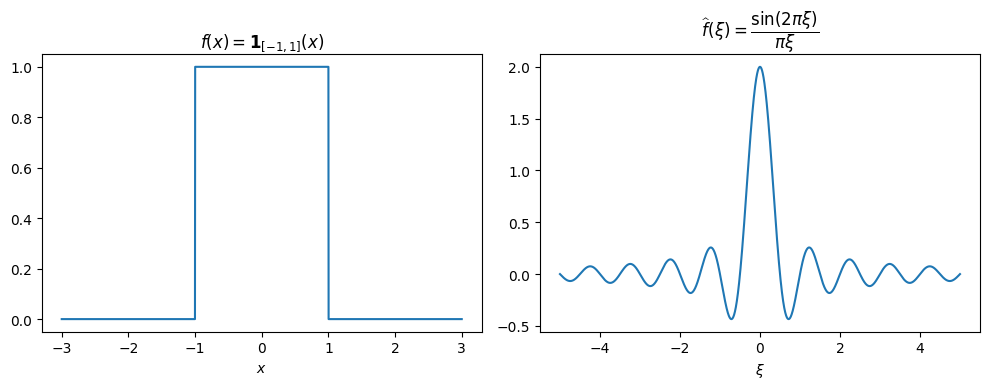
\includegraphics[width=0.7\textwidth]{transformada1.png}
  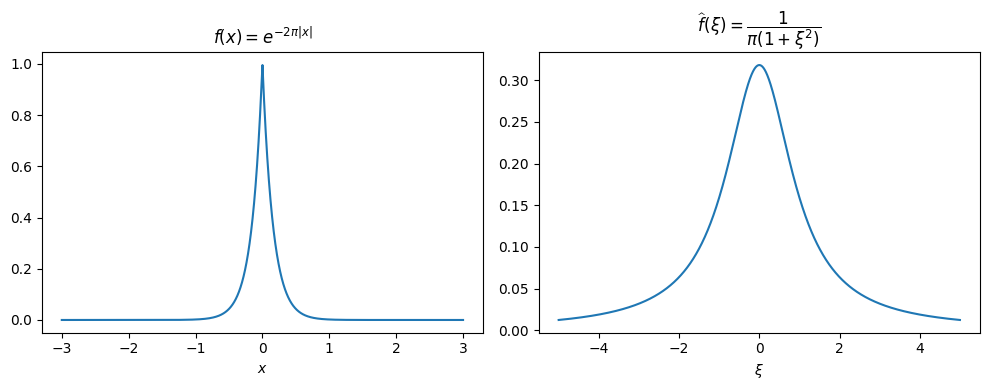
\includegraphics[width=0.7\textwidth]{transformada2.png}
  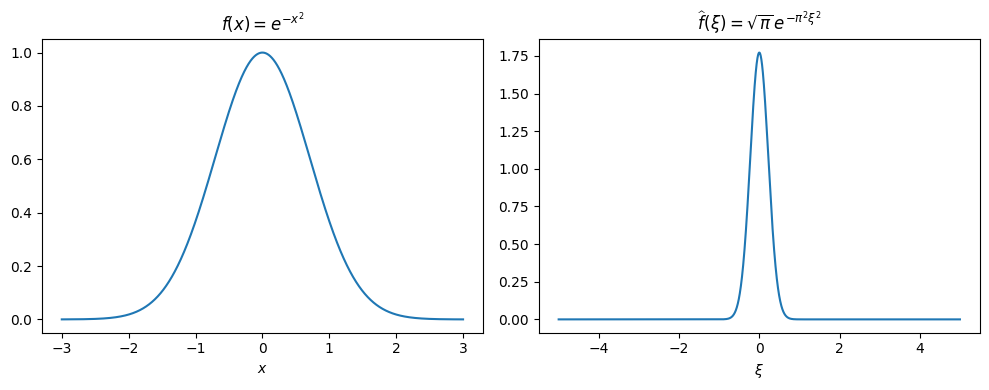
\includegraphics[width=0.7\textwidth]{transformada3.png}
  \caption{Gráficos de las funciones y sus transformadas en los ejemplos \ref{ej:indicadora}, \ref{ej:exponencial} y \ref{ej:gaussiana}.}
  \label{fig:transformadas}
\end{figure}

\section{Fórmula de inversión}

En esta sección daremos una demostración de la fórmula de inversión \eqref{fourier.inverse}. Este es el análogo para la transformada a los teoremas de convergencia de la serie de Fourier.

El objetivo de esta sección es probar el siguiente teorema:
\begin{teo}[Fórmula de inversión]
Sea $f\in L^1(\R)$ tal que $\hat f\in L^1(\R)$. Entonces
$$
f(x) = \int_{-\infty}^\infty \hat f(\xi)\, e^{2\pi i \xi x}\, d\xi
$$
en todo punto de continuidad de $f$.
\end{teo}

\begin{proof}
Hagamos primero la siguiente observación: Usando el Ejemplo \ref{ej:gaussiana} y el ítem 5 de la Proposición \ref{prop.algebraica}, tenemos que
\begin{equation}\label{gaussiana}
\widehat{e^{-\pi t^2\xi^2}}(y) = \tfrac{1}{t}e^{-\pi y^2/t^2}.
\end{equation}
Si ahora usamos el ítem 3 de la Proposición \ref{prop.algebraica} y el ítem 5 de la Proposición \ref{prop.analiticas} obtenemos
$$
\frac{1}{t} \int_{-\infty}^\infty f(x+y)\, e^{-\pi y^2/t^2}\, dy = \int_{-\infty}^\infty e^{-\pi t^2\xi^2} \hat f(\xi)\, e^{2\pi i\xi x}\, d\xi.
$$
Queremos ahora tomar límite cuando $t\to 0$ en esta igualdad.

Observemos que
$$
\lim_{t\to 0}\int_{-\infty}^\infty e^{-\pi t^2\xi^2} \hat f(\xi)\, e^{2\pi i\xi x}\, d\xi =  \int_{-\infty}^\infty \hat f(\xi)\, e^{2\pi i \xi x}\, d\xi
$$
que es el lado derecho de la fórmula de inversión. El paso al límite dentro de la integral se justifica fácilmente usando el Teorema de convergencia mayorada y que $\hat f\in L^1(\R)$.

Para la convergencia del otro término, primero observemos que, haciendo el cambio de variable $u=\sqrt{\pi}y/t$,
$$
\frac{1}{t}\int_{-\infty}^\infty e^{-\pi y^2/t^2}\, dy = \frac{1}{\sqrt{\pi}}\int_{-\infty}^\infty e^{-u^2}\, du =1,
$$
por el cálculo del Ejemplo \ref{ej:gaussiana}.

Luego
\begin{align*}
\frac{1}{t} \int_{-\infty}^\infty f(x+y)\, e^{-\pi y^2/t^2}\, dy - f(x) &= \frac{1}{t} \int_{-\infty}^\infty (f(x+y)- f(x))\, e^{-\pi y^2/t^2}\, dy\\
&= \int_{-\infty}^\infty (f(x+tu)-f(x)) e^{-\pi u^2}\, du
\end{align*}
Observemos que si $x$ es un punto de continuidad de $f$ el integrando tiende a 0 cuando $t\to 0$. Luego, podemos nuevamente usar el Teorema de convergencia mayorada para pasar al límite en la integral y concluir que
$$
\lim_{t\to 0}\frac{1}{t} \int_{-\infty}^\infty f(x+y)\, e^{-\pi y^2/t^2}\, dy = f(x),
$$
lo que culmina la demostración.
\end{proof}

\section{Transformada de Fourier y convolución}

Para terminar este capítulo, veamos cómo se comporta la transformada de Fourier con respecto a una operación central entre funciones integrables: el producto de convolución. Empecemos con la definición de convolución.
\begin{defi}
Si $f,g\in L^1(\R)$, definimos su convolución como
$$
(f*g)(x)=\int_{\R} f(x-y)\,g(y)\,dy.
$$
\end{defi}

Veamos que la convolución de dos funciones integrables, define una nueva función integrable.
\begin{lema}
Sean $f, g\in L^1(\R)$. Entonces $f*g\in L^1(\R)$ y tenemos
$$
\int_\R |(f*g)(x)|\, dx \le \int_\R |f(x)|\, dx \int_\R |g(x)|\, dx.
$$
\end{lema}

\begin{proof}
Observemos primero que
$$
|(f*g)(x)|\le \int_\R |f(x-y)|\, |g(y)|\, dy = (|f|*|g|)(x),
$$
luego, sin pérdida de generalidad podemos suponer que $f, g\ge 0$.

Ahora el resultado se desprende del Teorema de Fubini. En efecto,
\begin{align*}
\int_\R (f*g)(x)\, dx &= \int_\R \int_\R f(x-y)\, g(y)\, dy\, dx = \int_\R \int_\R f(x-y)\, g(y)\, dx\, dy\\
&= \int_\R g(y) \left(\int_\R f(x-y)\, dx\right)\, dy.
\end{align*}
La integral de $f$ es independiente del valor de $y\in\R$ por lo que obtenemos
$$
\int_\R (f*g)(x)\, dx = \left(\int_\R f(x)\, dx\right)\left(\int_\R g(y)\, dy\right),
$$
lo que finaliza la demostración.
\end{proof}

Ahora veamos cómo opera la transformada de Fourier con la convolución.

\begin{teo}[Teorema de la convolución]\label{trans.conv}
Sean $f,g\in L^1(\R)$, entonces
$$
\widehat{f*g}(\xi)=\hat f(\xi)\,\hat g(\xi) \quad\text{para todo }\xi\in\R.
$$
\end{teo}

\begin{proof}
Por definición,
$$
\widehat{f*g}(\xi) = \int_{\R}\int_{\R} f(x-y)\,g(y)\,e^{-2\pi i \xi x}\,dy\,dx.
$$
Usando Fubini y el cambio de variable $u=x-y$,
$$
\widehat{f*g}(\xi) = \int_{\R} g(y)\,e^{-2\pi i \xi y}\,dy \int_{\R} f(u)\,e^{-2\pi i \xi u}\,du = \hat f(\xi)\,\hat g(\xi).
$$
\end{proof}

Veremos en lo que resta de las notas varias aplicaciones de este resultado.

\section{El Teorema de Plancherel}

Hasta el momento hemos estudiado la transformada de Fourier para funciones integrables, es decir, pertenecientes a $L^1(\R)$. En ese contexto vimos que la transformada está bien definida y satisface propiedades fundamentales como la linealidad, la inversión y la transformación de derivadas en multiplicaciones. Sin embargo, en numerosas aplicaciones —particularmente en ecuaciones diferenciales, procesamiento de señales y mecánica cuántica— resulta natural trabajar con funciones que poseen energía finita, es decir, funciones pertenecientes a $L^2(\R)$, aun cuando no sean integrables.

El resultado central que permite extender la transformada de Fourier a este espacio es el teorema de Plancherel. Este establece que la transformada preserva exactamente la norma $L^2$, es decir,
$$
\|f\|_{L^2(\R)} = \|\widehat f\|_{L^2(\R)}.
$$
En otras palabras, la transformada de Fourier no altera la energía de una función, sino que simplemente la expresa en el dominio de las frecuencias. Desde un punto de vista geométrico, esto significa que la transformada es una isometría de $L^2(\R)$, propiedad que constituye uno de los pilares del análisis de Fourier moderno y que será una herramienta fundamental en el estudio de las ecuaciones en derivadas parciales.

\begin{teo}[Teorema de Plancherel]\label{Plancherel}
Sea $f\in L^1(\R)\cap L^2(\R)$. Entonces $\hat f\in L^2(\R)$ y
$$
\|f\|_{L^2(\R)} = \|\hat f\|_{L^2(\R)}.
$$
En consecuencia, la transformada de Fourier, definida en el subespacio denso $L^1(\R)\cap L^2(\R)$, se extiende de manera única a una isometría de $L^2(\R)$ en $L^2(\R)$.
\end{teo}

\begin{proof}
Hacemos la demostración bajo la hipótesis adicional de que $\hat f\in L^1(\R)$, que es la que permite usar la fórmula de inversión; el caso general se obtiene por un argumento de aproximación que puede verse en \cite{Duoandikoetxea}.

Por la fórmula de inversión, $f(x) = \int_\R \hat f(\xi)e^{2\pi i\xi x}\,d\xi$ en casi todo punto (en todo punto de continuidad, y $f$ coincide en casi todo punto con la función continua del lado derecho). Entonces, usando el Teorema de Fubini (que se aplica porque $\hat f\in L^1$ y $f\in L^1$),
\begin{align*}
\int_\R |f(x)|^2\, dx &= \int_\R f(x)\overline{f(x)}\, dx = \int_\R \left(\int_\R \hat f(\xi)\, e^{2\pi i \xi x}\, d\xi\right)\overline{f(x)}\, dx\\
&= \int_\R \hat f(\xi)\left(\int_\R \overline{f(x)}\, e^{2\pi i\xi x}\, dx\right) d\xi
= \int_\R \hat f(\xi)\,\overline{\left(\int_\R f(x)\, e^{-2\pi i\xi x}\, dx\right)}\, d\xi\\
&= \int_\R \hat f(\xi)\,\overline{\hat f(\xi)}\, d\xi = \int_\R |\hat f(\xi)|^2\, d\xi.
\end{align*}
La extensión a todo $L^2(\R)$ es consecuencia de que $L^1\cap L^2$ es denso en $L^2$ y de que una aplicación lineal que preserva la norma en un subespacio denso se extiende, de manera única y preservando la norma, a todo el espacio.
\end{proof}

\begin{obs}
Con el mismo argumento se prueba la \emph{identidad de Parseval}: si $f,g\in L^1(\R)\cap L^2(\R)$,
$$
\int_\R f(x)\overline{g(x)}\, dx = \int_\R \hat f(\xi)\overline{\hat g(\xi)}\, d\xi .
$$
La transformada de Fourier preserva no sólo la ``energía'' sino el producto interno: es la versión continua de la ortogonalidad de las exponenciales que usamos en las series de Fourier.
\end{obs}



\chapter{La transformada de Fourier discreta}\label{chap:DFT}

\section{Introducción}
En los capítulos anteriores estudiamos la transformada de Fourier en un marco continuo, tanto para funciones periódicas (series de Fourier) como para funciones definidas en todo $\R$. Sin embargo, en la práctica, los datos con los que se trabaja en aplicaciones reales son necesariamente discretos y finitos: señales muestreadas en el tiempo, imágenes digitales, registros experimentales o salidas de simulaciones numéricas.

La transformada de Fourier discreta (DFT, por sus siglas en inglés) surge como el análogo natural de la transformada de Fourier continua cuando se considera una señal dada por una cantidad finita de muestras igualmente espaciadas. Desde el punto de vista matemático, la DFT puede interpretarse como una expansión de un vector complejo en una base ortogonal de exponenciales discretas. Desde el punto de vista computacional, constituye la herramienta central para el análisis espectral de datos discretos.

En este capítulo introduciremos la definición de la transformada de Fourier discreta, discutiremos sus propiedades fundamentales y su relación con la transformada de Fourier continua. Prestaremos especial atención a su interpretación algebraica y geométrica, así como a los efectos del muestreo y la periodicidad implícita que introduce la discretización.

Finalmente, presentaremos la transformada rápida de Fourier (FFT), un algoritmo que permite calcular la DFT de manera eficiente y que resulta indispensable en aplicaciones modernas de procesamiento de señales, análisis de datos y simulación numérica.

\section{Definición y propiedades elementales}


Consideraremos funciones definidas sobre un conjunto finito discreto $0\le k\le N-1$ a valores en $\C$. Esto significa que tendremos elementos en $\C^N$, pero para mantener una analogía con lo que estudiamos en el caso continuo notaremos a estas funciones como $f[k]$. Resulta conveniente extender estas funciones periódicamente a $k\in\Z$ de la forma $f[k+N]=f[k]$ para todo $k$.

La transformada de Fourier discreta asocia a cada $f$ otra función $\hat f$ definida como
\begin{equation}\label{DFT}
\hat f[k] = \sum_{j=0}^{N-1} f[j]\, e^{-2\pi i jk/N}.
\end{equation}
Observemos que con esta definición tenemos que $\hat f[k+N] = \hat f[k]$ para todo $k$, es decir que podemos considerar a $\hat f$ como un elemento de $\C^N$ o como una sucesión periódica de período $N$.

Veamos la propiedades elementales de la transformada discreta.
\begin{prop}
Sea $f\in \C^N$ y $\hat f$ la transformada discreta dada por \eqref{DFT}. Entonces
\begin{enumerate}
\item La transformada discreta es una transformación lineal de $\C^N$ en $\C^N$.

\item \textbf{Traslación en el tiempo:} Si $g[k] = f[k-n]$, entonces $\hat g[k] = \hat f[k]\, e^{-2\pi ikn/N}$.

\item \textbf{Traslación en frecuencia:} Si $g[k] = f[k]\, e^{2\pi i kn/N}$, entonces $\hat g[k] = \hat f[k-n]$.
\end{enumerate}
\end{prop}
La demostración de esta proposición es elemental y queda de ejercicio al lector.

\section{Representación matricial de la transformada discreta}\label{sec:matricial}

Llamemos $\omega = e^{-2\pi i/N}$. Entonces $\bar \omega = \omega^{-1}$. Además tenemos que $\omega^j$ son raíces $N-$ésimas de la unidad para todo $j\in\N$, i.e. $\omega^{jN}=1$. Adicionalmente, tenemos que
$$
1+\omega^j + \omega^{2j} + \cdots + \omega^{(N-1)j} = \begin{cases}
N & \text{si $j$ es un múltiplo de $N$},\\
0 & \text{en otro caso}.
\end{cases}
$$
Esta es una consecuencia directa de la factorización 
$$
1-x^N = (1-x)(1+x+x^2+\cdots+x^{N-1}).
$$

Con esta notación, la transformada discreta \eqref{DFT} se escribe como
$$
\hat f[k] = \sum_{j=0}^{N-1} f[j] \omega^{jk}.
$$
Como la transformada discreta es una transformación lineal de $\C^N$ en $\C^N$, la misma tiene una representación matricial. Llamemos $\ff = (f[0],\dots,f[N-1])^t$ y $\hat \ff = (\hat f[0],\dots,\hat f[N-1])^t$. Entonces \eqref{DFT} se escribe como
$$
\hat\ff = A(\omega)\ff,
$$
donde $A(\omega)\in \C^{N\times N}$ viene dada por
$$
A(\omega) = \begin{bmatrix}
1 & 1 & 1 & \cdots & 1\\
1 & \omega & \omega^2 & \cdots & \omega^{N-1}\\
1 & \omega^2 & \omega^4 & \cdots & \omega^{2(N-1)}\\
\vdots & \vdots & \vdots & \ddots & \vdots\\
1 & \omega^{N-1} & \omega^{2(N-1)} & \cdots & \omega^{(N-1)(N-1)}
\end{bmatrix}.
$$
La matriz $A(\omega)$ es una matriz de Vandermonde asociada a las raíces $N$-ésimas de la unidad y codifica el cambio de coordenadas entre la base canónica y la base de exponenciales discretas.


\section{Transformada discreta inversa}

Observemos que, dado que $\bar \omega = \omega^{-1}$ es fácil ver que 
$$
A(\omega)A(\bar\omega) = A(\bar\omega)A(\omega) = N I_N,
$$
donde $I_N$ es la matriz identidad. Entonces
$$
\ff = \frac{1}{N} A(\bar\omega)\hat \ff,
$$
en otras palabras,
\begin{equation}\label{inversion.discreta}
f[k] = \frac{1}{N}\sum_{j=0}^{N-1} \hat f[j] \, \omega^{-jk} = \frac{1}{N}\sum_{j=0}^{N-1} \hat f[j] \, e^{2\pi i jk/N},
\end{equation}
que es la fórmula de inversión discreta.

\section{Transformada discreta en señales continuas}

Supongamos que tenemos una función $f$ definida periódica de período $T$ y queremos representarla en el intervalo $[0,T]$ por un polinomio trigonométrico de la forma
$$
p(x) = \sum_{j=0}^{N-1} c_j\, e^{2\pi i jx/T}.
$$
Al tener $N$ coeficientes, podemos hacerlo coincidir con la función $f$ en $N$ puntos (es decir, buscamos que $p$ interpole $f$ en $N$ puntos). Supongamos que los elegimos equiespaciados, es decir $x_k = kT/N$ con $k=0,1,\dots,N-1$, los coeficientes $c_j$ se determinan resolviendo el sistema
$$
f(\tfrac{kT}{N}) = \sum_{j=0}^{N-1} c_j\, e^{2\pi i jk/N}.
$$
Entonces, si llamamos $f[k]=f(\tfrac{kT}{N})$, la fórmula de inversión \eqref{inversion.discreta} nos da
$$
c_j = \frac{\hat f[j]}{N}.
$$

\section{Propiedades adicionales}

Veamos que la transformada discreta \eqref{DFT} verifica la identidad de Plancherel que vimos para series de Fourier (Corolario \ref{plancherel}).

Para eso necesitamos un pequeño lema cuya demostración queda para el lector.
\begin{lema}
Para $k,l\in\{0,\dots,N-1\}$ se cumple
$$
\sum_{j=0}^{N-1} e^{2\pi i j(k-l)/N} = 
\begin{cases}
N & \text{si } k=l,\\
0 & \text{si } k\neq l.
\end{cases}
$$
\end{lema}
Esto muestra que las exponenciales discretas forman una familia ortogonal en $\C^N$.

\begin{teo}
La transformada discreta de Fourier verifica
$$
\sum_{k=0}^{N-1} f[k]\, \overline{g[k]} = \frac{1}{N}\sum_{k=0}^{N-1} \hat f[k]\, \overline{\hat g[k]}.
$$
En particular
$$
\sum_{k=0}^{N-1} |f[k]|^2 = \frac{1}{N}\sum_{k=0}^{N-1} |\hat f[k]|^2.
$$
\end{teo}

\begin{proof}
Usemos la notación matricial de la Sección \ref{sec:matricial}. Observemos que $A(\omega)$ es simétrica y que $\overline{A(\omega)} = A(\bar \omega)$. 

Sean $\ff = (f[0],\dots, f[N-1])^t$ y $\gb = (g[0],\dots,g[N-1])^t$. Luego,
$$
\frac{1}{N}\sum_{k=0}^{N-1} \hat f[k]\, \overline{\hat g[k]} = \frac{1}{N}\hat \ff^t \overline{\hat \gb} = \frac{1}{N} (A(\omega)\ff)^t \overline{A(\omega)\gb} = \frac{1}{N} \ff^t A(\omega)A(\bar\omega)\bar\gb = \ff^t\gb = \sum_{k=0}^{N-1} f[k]\, \overline{g[k]} 
$$
\end{proof}

\begin{obs}
La identidad de Plancherel muestra que, salvo una constante de normalización, la DFT preserva el producto interno en $\C^N$.
\end{obs}
Para terminar veamos la versión discreta de la convolución y como es el comportamiento de la transformada discreta respecto a la misma. Comparar con el Teorema \ref{trans.conv}.


\begin{defi}
Sean $\ff, \gb\in\C^N$. Definimos la convolución $\ff*\gb$ como
$$
(f*g)[k] = \sum_{j=0}^{N-1} f[j]\, g[k-j]
$$
donde asumimos a $\gb$ extendida por periodicidad.
\end{defi}

Tenemos entonces
\begin{teo}
Sean $\ff, \gb\in\C^N$. Entonces
$$
\widehat{(f*g)}[k] = \hat f[k]\, \hat g[k].
$$
\end{teo}

\begin{proof}
La demostración es una aplicación directa de las definiciones. En efecto,
\begin{align*}
\widehat{(f*g)}[k] &= \sum_{j=0}^{N-1} (f*g)[j]\, \omega^{jk} = \sum_{j=0}^{N-1}\left(\sum_{l=0}^{N-1} f[l]\, g[j-l]\right) \omega^{jk}\\ 
&= \sum_{j=0}^{N-1} \sum_{l=0}^{N-1} f[l]\, \omega^{lk}\, g[j-l]\, \omega^{(j-l)k}\\
&= \hat f[k]\, \hat g[k].
\end{align*}
\end{proof}

\section{Periodicidad, muestreo y aliasing}

Un aspecto fundamental de la transformada de Fourier discreta es que introduce, de manera implícita, dos hipótesis estructurales sobre la señal analizada: \emph{periodicidad} y \emph{muestreo uniforme}. Estas hipótesis, si bien naturales desde el punto de vista computacional, tienen consecuencias importantes que deben ser tenidas en cuenta al interpretar los resultados de la DFT.

En primer lugar, al trabajar con una sucesión finita $f[0],\dots,f[N-1]$ y extenderla periódicamente mediante la convención $f[k+N]=f[k]$, se está asumiendo que la señal original es periódica de período $N$. En consecuencia, la DFT no analiza una señal aislada, sino una repetición infinita de la misma. Esta periodicidad implícita se
manifiesta, por ejemplo, en el hecho de que la convolución discreta definida en la Sección anterior es una \emph{convolución circular}.

En segundo lugar, la DFT puede interpretarse como el análisis espectral de una señal continua que ha sido muestreada en $N$ puntos equiespaciados. Desde este punto de vista, las frecuencias accesibles quedan restringidas a un conjunto finito de valores discretos. Frecuencias más altas que cierto umbral no pueden distinguirse de otras frecuencias más bajas, ya que producen las mismas muestras discretas. Este fenómeno se conoce como \emph{aliasing}.

De manera informal, el aliasing ocurre cuando la tasa de muestreo no es suficientemente alta para capturar las oscilaciones presentes en la señal original. Como consecuencia, componentes de alta frecuencia ``se pliegan'' sobre el espectro de bajas frecuencias, distorsionando la información espectral obtenida mediante la DFT. Este efecto no es un artefacto numérico, sino una limitación estructural del proceso de muestreo.

El estudio detallado de estas cuestiones conduce al teorema de muestreo de Nyquist--Shannon, que establece condiciones bajo las cuales una señal continua puede ser reconstruida a partir de sus muestras discretas sin pérdida de información. Si bien no desarrollaremos este resultado en estas notas, es importante tener en cuenta que la interpretación correcta de la DFT requiere comprender las hipótesis de periodicidad y muestreo que la subyacen, así como los posibles efectos de aliasing asociados a ellas.

En la Figura~\ref{fig:aliasing} se ilustra el fenómeno de aliasing. Los puntos negros representan una señal discreta obtenida mediante muestreo uniforme. Se muestran dos señales continuas distintas que interpolan exactamente los mismos datos discretos.
\begin{figure}[ht]
\centering
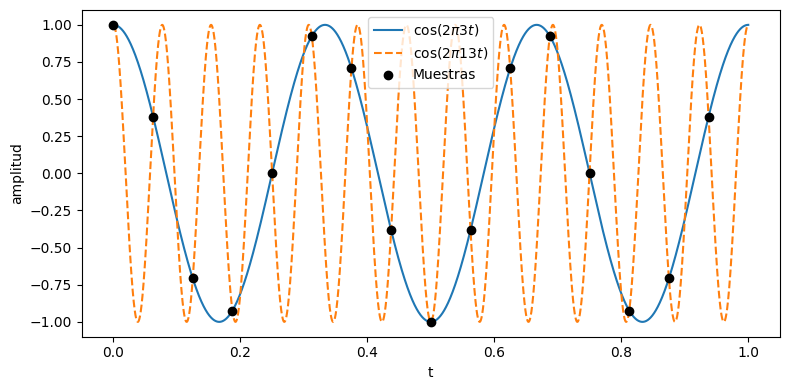
\includegraphics[width=0.8\textwidth]{aliasing.png}
\caption{Ejemplo de aliasing: dos señales continuas con distintas frecuencias producen las mismas muestras discretas cuando la tasa de muestreo es insuficiente.}
\label{fig:aliasing}
\end{figure}

Como la transformada de Fourier discreta sólo depende de los valores muestreados, no es posible distinguir cuál de las dos señales fue la original. Este ejemplo muestra que el aliasing no es un problema numérico, sino una consecuencia estructural del muestreo insuficiente.

\subsection*{La grilla de frecuencias y la frecuencia de Nyquist}

Conviene tener a mano el diccionario entre los índices de la DFT y las frecuencias físicas. Si la señal continua se muestrea durante un tiempo total $T$ con $N$ muestras equiespaciadas (paso $\Delta t = T/N$, tasa de muestreo $f_s = 1/\Delta t = N/T$), el coeficiente $\hat f[k]$ corresponde a la frecuencia
$$
\xi_k = \frac{k}{T} = \frac{k f_s}{N},\qquad k=0,1,\dots,N-1 .
$$
Dos consecuencias:
\begin{itemize}
\item La \emph{resolución} en frecuencia es $1/T$: para distinguir dos frecuencias que difieren en $\Delta\xi$ hay que observar la señal durante un tiempo $T\ge 1/\Delta\xi$. No importa cuán rápido se muestree; lo que da resolución es la duración del registro.
\item Por la periodicidad $\hat f[k+N]=\hat f[k]$ y, para señales reales, la simetría $\hat f[N-k] = \overline{\hat f[k]}$, los índices $k>N/2$ no traen información nueva: corresponden a las frecuencias negativas $\xi_k - f_s$. La frecuencia más alta que la DFT puede representar es
$$
\xi_{N/2} = \frac{f_s}{2},
$$
la \emph{frecuencia de Nyquist}. Una componente de la señal continua con frecuencia $\xi>f_s/2$ no desaparece: aparece en el espectro discreto en la frecuencia $|\xi - m f_s|$ más cercana a cero (para algún entero $m$), ``disfrazada'' de una frecuencia baja. Eso es el aliasing de la Figura~\ref{fig:aliasing}: allí la tasa de muestreo es $f_s=16$, y la frecuencia $13$ se pliega sobre $|13-16| = 3$.
\end{itemize}
La regla práctica es la del \emph{teorema de muestreo de Nyquist--Shannon}: para capturar sin distorsión una señal cuyas frecuencias no superan $\xi_{\max}$, hay que muestrear a más del doble, $f_s>2\xi_{\max}$. Si no se puede, hay que filtrar la señal (eliminar las frecuencias altas) \emph{antes} de muestrearla, porque después ya no se puede distinguir lo verdadero de lo plegado.

\begin{volvemos}{la señal de temperatura}
Un año de mediciones horarias tiene $N=8760$ muestras, $T=1$ año y $f_s = 8760$ ciclos por año ($24$ por día). La resolución es $1$ ciclo por año: el ciclo anual es el índice $k=1$ y el ciclo diario el índice $k=365$; sus armónicos (por ejemplo, el de $12$ horas, $k=730$) también son accesibles. La frecuencia de Nyquist es $12$ ciclos por día: cualquier variación más rápida que dos horas se pliega sobre frecuencias más bajas. Si en cambio tuviéramos una medición diaria a las 15 h, $f_s = 365$ ciclos por año, y el ciclo diario, de frecuencia $365$, quedaría plegado exactamente sobre la frecuencia $0$: se vería como un desplazamiento de la media (la temperatura a las 15 h es más alta que la media diaria) y no como una oscilación. Esto responde la tercera pregunta de la Sección \ref{sec:conductor-senal}: muestrear una vez por día no ``pierde'' el ciclo diario, lo \emph{confunde} con la media.
\end{volvemos}

\section{Transformada rápida de Fourier}

Desde la sección anterior vimos cómo el muestreo de una señal continua conduce naturalmente a la transformada discreta de Fourier (DFT), y discutimos el fenómeno de \emph{aliasing} como una consecuencia inevitable de trabajar con un número finito de muestras. En particular, observamos que la DFT no ``descubre'' frecuencias intrínsecas de la señal original, sino que organiza la información contenida en los datos muestreados de acuerdo con la escala temporal impuesta por el paso de muestreo.

Desde el punto de vista computacional, sin embargo, la definición directa de la DFT presenta una dificultad adicional: su evaluación requiere del orden de $N^2$ operaciones para una señal de longitud $N$. Este costo resulta prohibitivo en aplicaciones modernas, donde $N$ puede ser muy grande.

Afortunadamente, la DFT posee una estructura algebraica muy rica. En particular, las propiedades de las raíces de la unidad permiten factorizar recursivamente la matriz asociada a la DFT y reorganizar el cálculo de manera mucho más eficiente.

En este capítulo mostraremos que, explotando esta estructura, es posible computar la DFT en un tiempo del orden de $N \log N$. El algoritmo resultante, conocido como \emph{transformada rápida de Fourier} (FFT), constituye una de las herramientas fundamentales del análisis numérico moderno y es central en el procesamiento de señales, la ciencia de datos y numerosas aplicaciones científicas.

La transformada rápida de Fourier (FFT) adquirió su forma moderna a mediados del siglo XX, a partir del trabajo seminal de J. W. Cooley y J. W. Tukey, publicado en 1965 \cite{CooleyTukey}. En ese artículo, los autores mostraron que la transformada discreta de Fourier podía computarse de manera eficiente mediante un procedimiento recursivo que explota la factorización del tamaño de la señal y las propiedades de las raíces de la unidad. Este resultado redujo drásticamente el costo computacional de la DFT, de orden $N^2$ a orden $N \log N$, y tuvo un impacto inmediato en áreas como el procesamiento digital de señales, la física computacional y, más tarde, la ciencia de datos.

Sin embargo, el núcleo matemático del algoritmo es considerablemente más antiguo. Ya a comienzos del siglo XIX, Carl Friedrich Gauss había desarrollado un método esencialmente equivalente para calcular de manera eficiente coeficientes asociados a series trigonométricas, en el contexto de sus trabajos sobre interpolación y astronomía \cite{Gauss1805, Heideman}. Estas ideas permanecieron en gran medida desconocidas fuera de círculos especializados durante más de un siglo. El trabajo de Cooley y Tukey no sólo redescubrió y sistematizó estas técnicas, sino que las presentó en un lenguaje algorítmico acorde a la computación moderna, lo que explica su enorme difusión e influencia.

\subsection{El algoritmo}

Asumamos que $N$ es par. Entonces la idea es organizar el cálculo de la DFT de forma de que se realicen dos transformadas discretas en $\C^{N/2}$ y combinarlas adecuadamente para calcular la DFT en $\C^N$. Esto reduce el número de operaciones aproximadamente a la mitad. Luego, sucesivamente, se va iterando este proceso y al final el número de operaciones se reduce considerablemente. Esta es la idea de la FFT.

Antes de ver el caso general, veamos el caso $N=4$. Entonces $\omega=-i$ y la transformada es
$$
\begin{bmatrix}
\hat f[0]\\
\hat f[1]\\
\hat f[2]\\
\hat f[3]
\end{bmatrix}
= 
\begin{bmatrix}
1 & 1 & 1 & 1\\
1 & -i & -1 & i\\
1 & -1 & 1 & -1\\
1 & i & -1 & -i
\end{bmatrix}
\begin{bmatrix}
f[0]\\
f[1]\\
f[2]\\
f[3]
\end{bmatrix}.
$$

Escribamos este producto permutando las filas del lado derecho de manera tal que aparezcan primero los índices pares y luego los impares.
$$
\begin{bmatrix}
\hat f[0]\\
\hat f[1]\\
\hat f[2]\\
\hat f[3]
\end{bmatrix}
= 
\begin{bmatrix}
1 & 1 & 1 & 1\\
1 & -1 & -i & i\\
1 & 1 & -1 & -1\\
1 & -1 & i & -i
\end{bmatrix}
\begin{bmatrix}
f[0]\\
f[2]\\
f[1]\\
f[3]
\end{bmatrix}.
$$

Observemos que si llamamos $\ff_p = (f[0], f[2])$ a las coordenadas pares y $\ff_i = (f[1], f[3])$ a las impares, entonces esta última igualdad se puede escribir como
$$
\begin{bmatrix}
\hat f[0]\\
\hat f[1]
\end{bmatrix}
=
\begin{bmatrix}
1 & 1\\
1 & -1 
\end{bmatrix}
\begin{bmatrix}
f_p[0]\\
f_p[1]
\end{bmatrix}
+
\begin{bmatrix}
1 & 0\\
0 & -i 
\end{bmatrix}
\begin{bmatrix}
1 & 1\\
1 & -1 
\end{bmatrix}
\begin{bmatrix}
f_i[0]\\
f_i[1]
\end{bmatrix}
$$
y
$$
\begin{bmatrix}
\hat f[2]\\
\hat f[3]
\end{bmatrix}
=
\begin{bmatrix}
1 & 1\\
1 & -1 
\end{bmatrix}
\begin{bmatrix}
f_p[0]\\
f_p[1]
\end{bmatrix}
+
\begin{bmatrix}
-1 & 0\\
0 & i 
\end{bmatrix}
\begin{bmatrix}
1 & 1\\
1 & -1 
\end{bmatrix}
\begin{bmatrix}
f_i[0]\\
f_i[1]
\end{bmatrix}.
$$

Observemos que
$$
\begin{bmatrix}
1 & 1\\
1 & -1 
\end{bmatrix}
\begin{bmatrix}
f_p[0]\\
f_p[1]
\end{bmatrix}
=
\begin{bmatrix}
\hat f_p[0]\\
\hat f_p[1]
\end{bmatrix}\quad \text{y}\quad
\begin{bmatrix}
1 & 1\\
1 & -1 
\end{bmatrix}
\begin{bmatrix}
f_i[0]\\
f_i[1]
\end{bmatrix}
=
\begin{bmatrix}
\hat f_i[0]\\
\hat f_i[1]
\end{bmatrix},
$$
luego
\begin{align*}
\hat f[0] &= \hat f_p[0] + \hat f_i[0]\\
\hat f[1] &= \hat f_p[1] -i \hat f_i[1]\\
\hat f[2] &= \hat f_p[0] - \hat f_i[0]\\
\hat f[3] &= \hat f_p[1] + i \hat f_i[1].
\end{align*}

Es decir, redujimos el problema de calcular una DFT de dimensión 4 en el cálculo de 2 DFT de dimensión 2.

Veamos ahora el caso general, asumiendo que $N$ es par. El procedimiento es bastante similar, sólo que la notación se vuelve más complicada.

La primera parte consiste en reordenar el vector $\ff$ poniendo las coordenadas pares primero y las coordenadas impares después. Así tenemos $\ff_p = (f_p[0],\dots,f_p[N/2-1])^t = (f[0], f[2],\dots,f[N-2])^t$ y $\ff_i = (f_i[0],\dots,f_i[N/2])^t = (f[1], f[3], \dots, f[N-1])^t$. Luego escribimos
$$
\hat \ff = \begin{bmatrix}
\hat f[0]\\
\hat f[1]\\
\vdots\\
\hat f[\tfrac{N}{2}-1]\\
\hat f[\tfrac{N}{2}]\\
\hat f[\tfrac{N}{2}+1]\\
\vdots \\
\hat f[N-1]
\end{bmatrix} = 
A(\omega)\ff = 
R(\omega) \begin{bmatrix}
\ff_p\\
\ff_i
\end{bmatrix} = 
R(\omega) \begin{bmatrix}
f[0]\\
f[2]\\
\vdots\\
f[N-2]\\
f[1]\\
f[3]\\
\vdots\\
f[N-1]
\end{bmatrix},
$$
donde la matriz $R(\omega)$ viene dada por
$$
R(\omega)= \begin{bmatrix}
1 & 1 & \cdots & 1 & 1 & 1 & \cdots & 1\\
1 & \omega^2 & \cdots & \omega^{N-2} & \omega & \omega^3 & \cdots & \omega^{N-1}\\
\vdots & \vdots & \ddots & \vdots & \vdots & \vdots & \ddots & \vdots\\
1 & \omega^{N-2} & \cdots & \omega^{(\frac{N}{2}-1)^2} & \omega^{\frac{N}{2}-1} & \omega^{3(\frac{N}{2}-1)} & \cdots &\omega^{(\frac{N}{2}-1)\frac{N}{2}}\\
1 & 1 & \cdots & 1 & -1 & -1 & \cdots & -1\\
1 & \omega^2 & \cdots & \omega^{N-2} & -\omega & -\omega^3 & \cdots & -\omega^{N-1}\\
\vdots & \vdots & \ddots & \vdots & \vdots & \vdots & \ddots & \vdots\\
1 & \omega^{N-2} & \cdots & \omega^{(\frac{N}{2}-1)^2} & -\omega^{\frac{N}{2}-1} &- \omega^{3(\frac{N}{2}-1)} & \cdots & -\omega^{(\frac{N}{2}-1)\frac{N}{2}}
\end{bmatrix}.
$$
Para deducir la expresión para $R(\omega)$ se usa que $\omega^N=1$ en las primeras $N/2$ columnas y que $\omega^{N/2}=-1$ en las segundas $N/2$ columnas.

Observemos que la matriz $R(\omega)$ es una matriz de 4 bloques de $(N/2)\times(N/2)$ de la forma
$$
R(\omega) = \left[
\begin{array}{c|c}
A_{N/2}(\omega) & D_{N/2}(\omega)A_{N/2}(\omega) \\ \hline
A_{N/2}(\omega) & -D_{N/2}(\omega)A_{N/2}(\omega)
\end{array}
\right],
$$ 
donde
$$
A_{N/2}(\omega) = \begin{bmatrix}
1 & 1 & \cdots & 1\\
1 & \omega^2 & \cdots & \omega^{N-2}\\
\vdots & \vdots & \ddots & \vdots\\
1 & \omega^{N-2} & \cdots & \omega^{(\frac{N}{2}-1)^2} 
\end{bmatrix}
$$
que es la matriz de DFT en dimensión $N/2$ y 
$$
D_{N/2}(\omega) = \begin{bmatrix}
1 & 0 & \cdots & 0\\
0 & \omega & \cdots & 0\\
\vdots & \vdots & \ddots & \vdots\\
0 & 0 & \cdots & \omega^{\frac{N}{2}-1}
\end{bmatrix},
$$
es decir una matriz diagonal con entradas $\omega^j$.

Luego, como 
$$
A_{N/2}(\omega)\ff_p = \hat \ff_p \quad \text{y}\quad A_{N/2}(\omega)\ff_i = \hat \ff_i,
$$
al igual que en el caso $N=4$, llegamos a
$$
\hat f[j] = \hat f_p[j] + \omega^j \hat f_i[j]\quad \text{y}\quad \hat f[\tfrac{N}{2}+j] = \hat f_p[j] - \omega^j \hat f_i[j],
$$
para $j=0,\dots,\tfrac{N}{2}-1$.

Luego, hemos reducido el problema del cálculo de una DFT en dimensión $N$ al clálculo de la misma en dimensión $N/2$. Si ahora $N/2$ es nuevamente par podemos volver a aplicar el mismo argumento y reducir el cálculo a transformadas en dimensión $N/4$ y así sucesivamente.


\chapter{Aplicaciones del análisis de Fourier}\label{chap:aplicaciones}

En los capítulos anteriores desarrollamos el análisis de Fourier desde un punto de vista
teórico y algorítmico, culminando con la transformada discreta de Fourier y su cálculo
eficiente mediante la FFT. En este capítulo presentamos dos aplicaciones representativas
que ilustran cómo estas herramientas permiten extraer información relevante de datos
reales y simplificar su tratamiento.

El objetivo no es describir aplicaciones exhaustivas ni abordar modelos basados en
ecuaciones diferenciales parciales —que serán tratados más adelante—, sino mostrar
cómo la representación frecuencial permite separar escalas, filtrar información no
deseada y reducir la complejidad de los datos sin perder sus características esenciales.

Nos concentraremos en dos ejemplos clásicos: el filtrado de ruido en señales
unidimensionales y la compresión de imágenes mediante análisis espectral.

\section{Filtrado de ruido en señales unidimensionales}

Consideremos una señal unidimensional que resulta de la superposición de un número
finito de oscilaciones armónicas. Es decir, una señal de la forma
\[
s(t) = \sum_{j=1}^m a_j \cos(2\pi f_j t + \varphi_j),
\]
donde las frecuencias $f_j$ y amplitudes $a_j$ están bien separadas y representan el
contenido determinista de la señal.

En un contexto experimental, la señal observada rara vez coincide exactamente con
$s(t)$. En su lugar, se registra una señal perturbada por ruido,
\[
u(t) = s(t) + \eta(t),
\]
donde $\eta(t)$ modela ruido aleatorio, que idealizaremos como ruido blanco. Ver Figura \ref{fig:señal}.
\begin{figure}[ht]
  \centering
  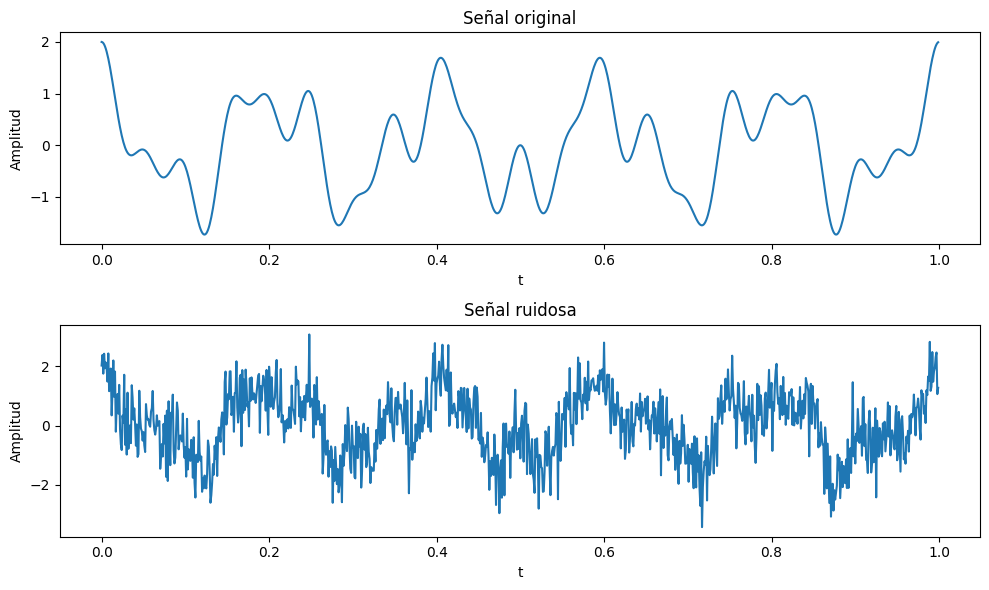
\includegraphics[width=0.7\textwidth]{señal1.png}
  \caption{Señal original y señal ruidosa.}
  \label{fig:señal}
\end{figure}

\subsection{Análisis espectral}

Al calcular la transformada discreta de Fourier de la señal observada $u(t)$, se obtiene
una representación espectral que combina dos comportamientos cualitativamente distintos.
Por un lado, las componentes armónicas de $s(t)$ se manifiestan como picos bien localizados
en frecuencias específicas. Por otro lado, el ruido blanco presenta un espectro distribuido
de manera aproximadamente uniforme sobre todo el rango de frecuencias.

Esta separación en el dominio frecuencial es la clave que permite distinguir señal de
ruido. Ver Figura \ref{fig:espectro-señal}.
\begin{figure}[ht]
  \centering
  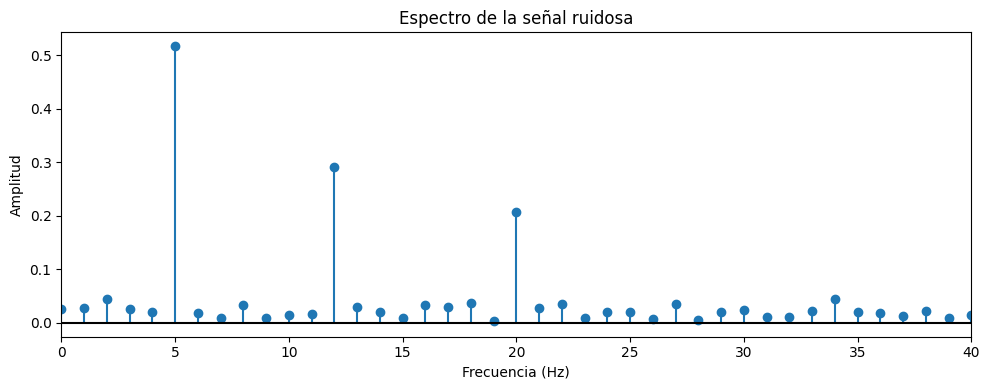
\includegraphics[width=0.7\textwidth]{espectro-señal.png}
  \caption{Análisis espectral de la señal ruidosa}
  \label{fig:espectro-señal}
\end{figure}



\subsection{Filtrado en el dominio de Fourier}

Una vez identificadas las frecuencias relevantes, es posible construir un filtro que
atenúe o elimine las componentes espectrales asociadas al ruido. En su forma más simple,
esto consiste en definir una función de transferencia $H(k)$ tal que
\[
\widehat{u}_{\mathrm{filtrada}}(k) = H(k)\,\hat u(k),
\]
donde $H(k)$ vale uno en un conjunto de frecuencias seleccionadas y cero fuera de él.

Aplicando luego la transformada inversa de Fourier, se obtiene una señal filtrada en el
dominio del tiempo que conserva las oscilaciones principales y elimina gran parte del
ruido. Este procedimiento ilustra cómo el análisis de Fourier permite diseñar filtros de
manera conceptualmente simple y computacionalmente eficiente. Ver la Figura \ref{fig:espectro-filtrado} para ver el filtro usado y la Figura \ref{fig:señal-filtrada} para ver la señal filtrada obtenida.
\begin{figure}[ht]
  \centering
  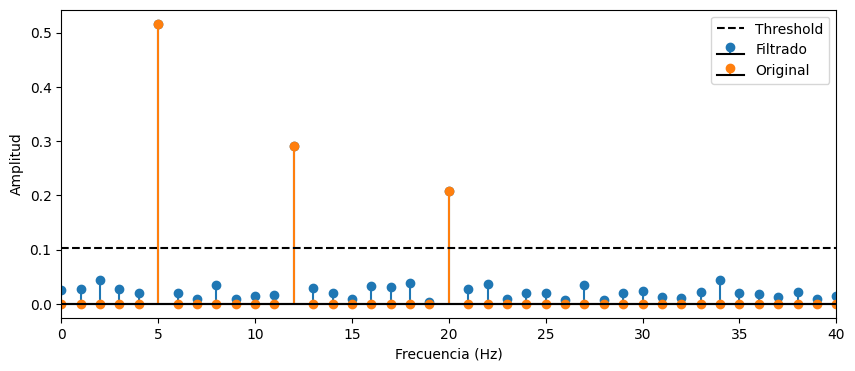
\includegraphics[width=0.7\textwidth]{espectro-filtrado.png}
  \caption{Filtro usado}
  \label{fig:espectro-filtrado}
\end{figure}
\begin{figure}[ht]
  \centering
  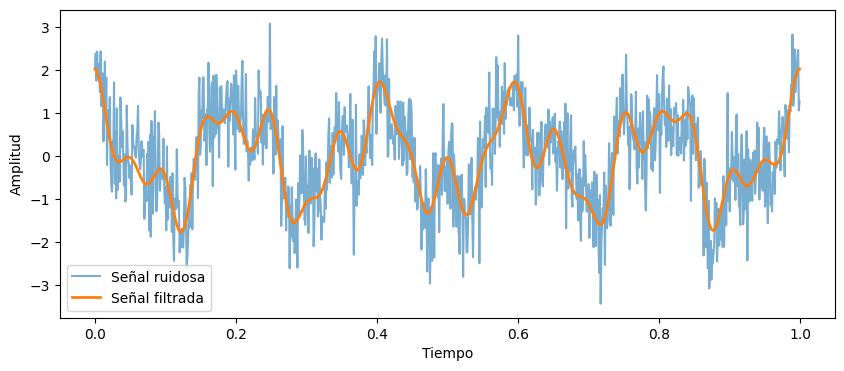
\includegraphics[width=0.7\textwidth]{señal-filtrada.png}
  \caption{Señal filtrada}
  \label{fig:señal-filtrada}
\end{figure}


\subsection{Aspectos prácticos: ventanas y espectro de potencia}

Dos observaciones prácticas sobre el análisis espectral de señales reales.

\paragraph{Fuga espectral y ventanas.} La DFT supone que la señal es periódica de período $T$ (la duración del registro). Una señal real casi nunca lo es: el valor final no coincide con el inicial y, al ``pegar'' periódicamente el registro, se introduce un salto. Ese salto tiene un espectro que decae lentamente (como $1/k$, por la discusión del Capítulo \ref{chap:conv.Fourier}), y contamina todas las frecuencias: un pico puro se ve rodeado de ``faldas'' que pueden tapar picos más débiles. Este efecto se llama \emph{fuga espectral} (\emph{leakage}). El remedio habitual es multiplicar la señal por una \emph{ventana} $w[j]$ que valga cero (o casi) en los extremos y uno en el centro (por ejemplo, la ventana de Hann, $w[j] = \frac12(1-\cos(2\pi j/N))$) antes de calcular la DFT. La señal ventaneada sí se pega bien periódicamente. El precio es una pérdida de resolución: el pico se ensancha. En el laboratorio se comparan varias ventanas.

\paragraph{Espectro de potencia.} Cuando la señal contiene ruido, la fase de los coeficientes $\hat u[k]$ es esencialmente aleatoria y lo que se estudia es su módulo al cuadrado, $|\hat u[k]|^2$, que por la identidad de Plancherel discreta representa la ``energía'' que la señal tiene en la frecuencia $\xi_k$. Normalizado adecuadamente se lo llama \emph{periodograma} o \emph{espectro de potencia}. El ruido blanco tiene un espectro de potencia aproximadamente plano, y una señal periódica, picos: es lo que muestra la Figura~\ref{fig:espectro-señal}. Para señales largas conviene además promediar los periodogramas de tramos sucesivos de la señal (método de Welch), lo que reduce la varianza del espectro estimado a costa de resolución.

\begin{volvemos}{la señal de temperatura}
Con la DFT y el espectro de potencia se responde la primera pregunta de la Sección \ref{sec:conductor-senal} de manera cuantitativa: los picos en $k=1$ y $k=365$ (y sus armónicos) dan las amplitudes de los ciclos anual y diario, y la fracción de la energía total (fuera de la media) contenida en esos picos dice cuánto de la variabilidad explican los ciclos; el resto es la parte irregular. La segunda pregunta se responde con un filtro: conservar sólo los coeficientes de los picos y antitransformar da la ``temperatura regular'', y la diferencia con la señal original es la parte irregular, cuyo espectro se puede analizar a su vez (¿es blanco, o tiene una estructura de escalas de días, que corresponde a los frentes meteorológicos?). La cuarta pregunta es la de la sección siguiente, aplicada a una señal en lugar de a una imagen: ¿con cuántos coeficientes se reconstruye la serie con un error del $5\%$?
\end{volvemos}

\section{Compresión de imágenes mediante análisis espectral}

Las imágenes digitales pueden interpretarse como funciones definidas sobre una grilla
bidimensional finita. Matemáticamente, una imagen en escala de grises puede modelarse
como una matriz $I \in \R^{N\times N}$, donde cada entrada representa la intensidad de un
píxel.

Desde el punto de vista computacional, esta información puede reorganizarse como un
vector en $\R^{N^2}$, lo que permite aplicar directamente las herramientas desarrolladas
para la transformada discreta de Fourier unidimensional. Si bien esta representación
pierde la estructura bidimensional explícita de la imagen, resulta suficiente para
poner de manifiesto fenómenos fundamentales vinculados a la distribución espectral de
la información.

\subsection{Contenido frecuencial de una imagen}

En el dominio de Fourier, las bajas frecuencias están asociadas a variaciones suaves de
intensidad, mientras que las altas frecuencias corresponden a cambios abruptos, bordes
y detalles finos.

En muchas imágenes naturales, los valores de intensidad presentan una fuerte correlación
espacial, lo que se traduce en una concentración muy marcada de la energía espectral en
un subconjunto reducido de coeficientes de Fourier. En consecuencia, la mayor parte del
espectro tiene amplitud muy pequeña y contribuye de manera marginal a la percepción
visual global de la imagen.

Este fenómeno se observa claramente al analizar el módulo de la transformada discreta
de Fourier del vector asociado a la imagen, donde sólo unos pocos coeficientes dominan
en magnitud.

\subsection{Compresión por truncamiento espectral}

Esta concentración espectral puede explotarse con fines de compresión. La idea básica
consiste en calcular la transformada de Fourier de la imagen, conservar únicamente un
cierto porcentaje de los coeficientes de mayor magnitud y anular el resto. A partir de
este espectro truncado, se reconstruye una imagen aproximada mediante la transformada
inversa.

Los ejemplos presentados muestran que, para imágenes naturales, incluso conservando una
fracción extremadamente pequeña de los coeficientes —del orden del $10^{-2}\%$ o menos—
la imagen reconstruida preserva la estructura visual global y resulta claramente
reconocible. Sólo cuando el porcentaje de coeficientes retenidos desciende aún más,
comienzan a aparecer distorsiones perceptibles. En la Figura \ref{fig:imagen-original} se puede ver la imagen original en escala de grises y en la Figura \ref{fig:compresion-imagen} se pueden ver las diferentes compresiones conservando el 3\%, 1\%, 0.1\% y 0.01\% de las frecuencias más relevantes en la descomposición de Fourier.

\begin{figure}[ht]
\centering
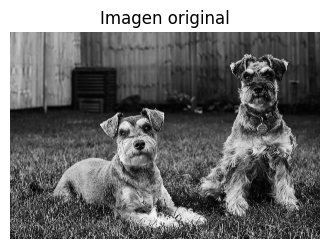
\includegraphics[width=0.45\textwidth]{imagen-original.png}
\caption{Imagen original en escala de grises.}
\label{fig:imagen-original}
\end{figure}

Este comportamiento pone de manifiesto que la información visual relevante se encuentra
altamente concentrada en el dominio frecuencial, y explica por qué los métodos de
compresión basados en transformadas, como los utilizados en el procesamiento digital de
imágenes, resultan tan eficaces.

\begin{figure}[ht]
\centering
\begin{tabular}{cc}
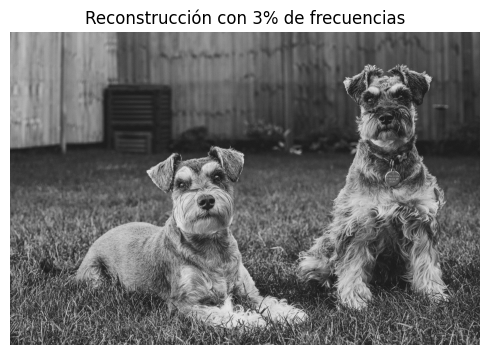
\includegraphics[width=0.4\textwidth]{imagen-3.png} &
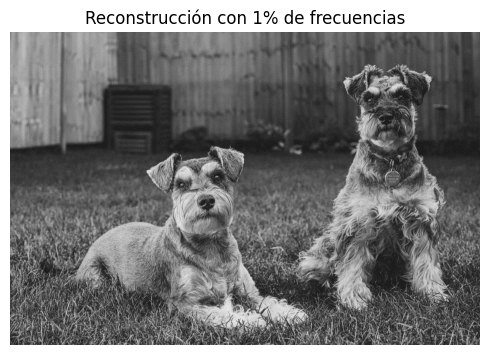
\includegraphics[width=0.4\textwidth]{imagen-1.png} \\
(a) 3\% de coeficientes &
(b) 1\% de coeficientes \\[0.5em]
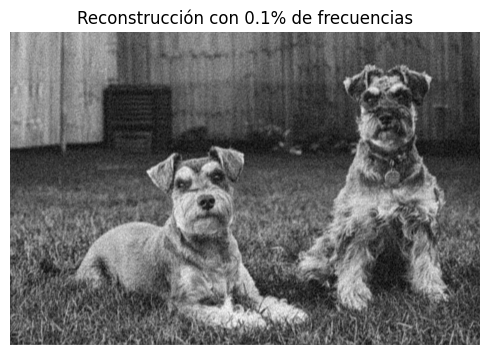
\includegraphics[width=0.4\textwidth]{imagen-01.png} &
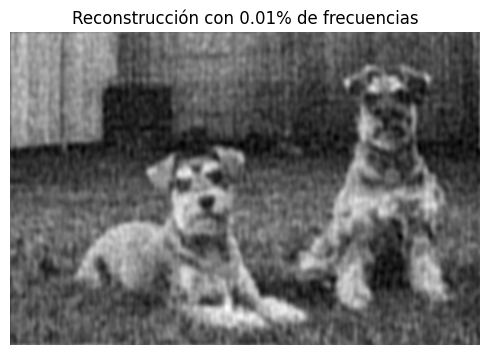
\includegraphics[width=0.4\textwidth]{imagen-001.png} \\
(c) 0.1\% de coeficientes &
(d) 0.01\% de coeficientes
\end{tabular}
\caption{Reconstrucción de la imagen mediante truncamiento espectral, conservando distintos porcentajes de los coeficientes de Fourier de mayor magnitud.}
\label{fig:compresion-imagen}
\end{figure}



\chapter{Ejercicios}
\section{Ejercicios teóricos}



\subsection*{Cálculo de series de Fourier y propiedades elementales}

\begin{ejer} \label{ejemplos}
Calcular los coeficientes de Fourier de las funciones periódicas de periodo $2\pi$ que siguen. Indicar en qué casos el criterio de Weierstrass permite asegurar la convergencia uniforme de las series que resultan:
\begin{enumerate}
\item $f(x)=x^2$ en $(-\pi,\pi)$;
 
\item $f(x)=x^2$ en $(0,2\pi)$;

\item $f(x) = |\sin x|$ en $(-\pi,\pi)$;

\item $f(x) = e^{ax}$ en $(-\pi,\pi)$ con $a\neq 0$;

\item $f(x) = \cos ax$ en $(-\pi,\pi)$ con $a$ no entero; 

\item $f(x) = \sin ax$ en $(-\pi,\pi)$ con $a$ no entero;

\item $f(x) = (\pi-x)\sin x$ en $(-\pi,\pi)$;

\item $f(x) =\begin{cases}
0 & \text{si } x \in (-\pi,0),\\ 
x & \text{si } x\in (0,\pi);
\end{cases}$

\item $f(x) = \begin{cases}
-e^{-x} & \text{si } x\in (-\pi, 0),\\
e^x & \text{si } x\in (0,\pi).
\end{cases}$
\end{enumerate}
\end{ejer}

\begin{ejer}
Escribir la serie de Fourier de la función periódica $f(x) =\left|\cos \frac{\pi x}{\ell}\right|$.
\end{ejer}

\begin{ejer}
Obtener los coeficientes de Fourier de la función
$$
f_\delta(x) = \begin{cases}
0 & \text{si } x \in (-\pi, \delta),\\
1/\delta & \text{si } x\in (-\delta, \delta),\\
0 & \text{si } x\in (\delta, \pi),
\end{cases}
$$
y calcular $\lim_{\delta\to 0} a_n(f_\delta)$ y $\lim_{\delta\to 0} b_n(f_\delta)$.
\end{ejer}

\begin{ejer}
Escribir la serie de Fourier de senos de la función $f(x) = \cos x$ en $(0, \pi)$.
\end{ejer}

\begin{ejer}
Escribir la serie de Fourier de cosenos de la función
$$
f(x) = \begin{cases}
1 & \text{si } x \in (0,h),\\
0 & \text{si } x\in (h,\pi).
\end{cases}
$$
\end{ejer}

\begin{ejer}
Escribir la serie de Fourier de senos y de cosenos de la función
$$
f(x)=\begin{cases}
\pi/3 & \text{si } x\in (0,\pi/3),\\
0 & \text{si } x\in (\pi/3, 2\pi/3),\\
-\pi/3 & \text{si } x\in (2\pi/3,\pi).
\end{cases}
$$
\end{ejer}


\begin{ejer}
\begin{enumerate}
\item Probar que si $f$ es una función $2\pi-$periódica de clase $C^1$ se tiene que los coeficientes de Fourier de $f$ y de $f'$ se relacionan mediante las expresiones
$$
a_k(f) = -\frac{b_k(f')}{k},\quad b_k(f) = \frac{a_k(f')}{k},\quad k=1,2,\dots
$$
Comprobar que es suficiente asumir que $f'$ exista y sea continua a trozos.

\item Supongamos que $f$ es continua excepto en el punto $x_0$ (y sus trasladados en múltiplos de $2\pi$) en el que tiene una discontinuidad de salto. Supongamos además que $f$ es derivable a trozos y que $f'$ es continua a trozos, ¿cuál es la relación entre los coeficientes de Fourier de $f$ y $f'$?
\end{enumerate}
\end{ejer}

 \begin{ejer}[Series de Fourier en forma compleja]
En este ejercicio relacionamos la forma real y la forma compleja de una serie de Fourier.

\begin{enumerate}
 \item Se considera el polinomio trigonométrico
 $$
 p_N(x)= \frac{a_0}{2} + \sum_{k=1}^N (a_k \cos kx + b_k \sin kx).
 $$
 Sustituyendo $\cos kx$ y $\sin kx$ por exponenciales complejas, verificar que se puede escribir de la forma
 $$
 p_N(x) = \sum_{k=-N}^N c_k e^{ikx},
 $$
 y expresar los coeficientes $c_k$ en términos de $a_k$ y $b_k$, y recíprocamente.
 
 \item Si los valores de $a_k$ y $b_k$ son todos reales, el polinomio $p_N$ toma sólo valores reales para $x\in\R$. Escribir una condición sobre los coeficientes $c_k$ para que $p_N(x)\in \R$ si $x\in\R$.

\item Calcular las integrales en $(-\pi,\pi)$ de los productos de funciones $e^{inx}$ y $e^{imx}$. Deducir las relaciones de ortogonalidad de la familia $\{e^{ikx}, k\in\Z\}$.

\item Supongamos que la función $f$ de período $2\pi$ se representa por la serie trigonométrica
 $$
 f(x) = \sum_{k=-\infty}^\infty c_k e^{ikx},
 $$
y que ésta es uniformemente convergente. A partir de las relaciones de ortogonalidad del ítem anterior, encontrar la expresión del {\em $k-$ésimo coeficiente de Fourier} $c_k$,
$$
c_k = \frac{1}{2\pi} \int_{-\pi}^\pi f(x)e^{-ikx}\, dx.
$$

\item Deducir las siguientes propiedades para los coeficientes $c_k$ análogas a las de los coeficientes $a_k$ y $b_k$:
\begin{enumerate}
\item $|c_k|\le \frac{1}{2\pi} \int_{-\pi}^\pi |f(x)|\, dx$, donde $|c_k|$ es el módulo del número complejo $c_k$;
\item $c_k(f')=ik c_k(f)$.
\end{enumerate}

\item Obtener la desigualdad de Bessel
$$
\sum_{k=-\infty}^\infty |c_k|^2 \le \frac{1}{2\pi} \int_{-\pi}^\pi |f(x)|^2\, dx,
$$
razonando igual a como lo hicimos para polinomios trigonométricos reales.
\end{enumerate}
\end{ejer}

\subsection*{Convergencia de la serie de Fourier}

\begin{ejer}
Estudiar si las funciones del ejercicio \ref{ejemplos} verifican alguna de las hipótesis que garantizan la convergencia de las series de Fourier asociadas.
\end{ejer}

\begin{ejer}
Calcular la serie de Fourier de $f(x)=Ax^2+Bx$ definida para $x\in (0,2\pi)$ y utilizarla para calcular las siguientes sumas:
$$
\sum_{k=1}^\infty \frac{\sin kx}{k},\quad \sum_{k=1}^\infty \frac{\cos kx}{k^2},\quad \sum_{k=1}^\infty \frac{1}{k^2}(\cos kx - k\pi \sin kx).
$$
\end{ejer}

\begin{ejer}
Comprobar que de la serie de Fourier de $\operatorname{sg} x$ se obtiene la de $|x|$ por integración término a término.
\end{ejer}

\begin{ejer}
Integrando la serie de Fourier de $f(x)=x$ en $(-\pi, \pi)$ demostrar que para $-\pi\le x\le \pi$, se tiene
$$
x^2 = \frac{\pi^2}{3} - 4 \left(\frac{\cos x}{1^2} - \frac{\cos 2x}{2^2} + \frac{\cos 3x}{3^2} - \cdots \right)
$$
y, a partir de esta, demostrar que para $-\pi\le x\le \pi$,
$$
x(\pi - x)(\pi + x) = 12 \left(\frac{\sin x}{1^3} - \frac{\sin 2x}{2^3} + \frac{\sin 3x}{3^3}-\cdots\right),
$$
con convergencia uniforme en ambos casos.
\end{ejer}

\begin{ejer}
Verificar las siguientes expansiones
$$
x=2\left(\sin x - \frac{\sin 2x}{2} + \frac{\sin 3x}{3} - \cdots \right)
$$
y 
$$
x^2 = \frac{\pi^2}{3} - 4\left(\cos x - \frac{\cos 2x}{2^2} + \frac{\cos 3x}{3^2} - \cdots\right)
$$
y usar la identidad de Plancherel para deducir las sumas
$$
\sum_{k=1}^\infty \frac{1}{k^2} = \frac{\pi^2}{6} \quad \text{y}\quad \sum_{k=1}^\infty \frac{1}{k^4} = \frac{\pi^4}{90}.
$$
\end{ejer}

\begin{ejer}
Escribir la identidad de Plancherel para la función
$$
f(x) = \begin{cases}
1 & \text{si } |x|<\alpha,\\
0 & \text{si } \alpha < |x| < \pi.
\end{cases}
$$
Calcular las sumas de las series
$$
\sum_{k=1}^\infty \frac{\sin^2 k\alpha}{k^2} \quad \text{y}\quad \sum_{k=1}^\infty \frac{\cos^2 k\alpha}{k^2}.
$$
\end{ejer}

\subsection*{La transformada de Fourier}

\begin{ejer}
Dos maneras de calcular la integral de $e^{-\pi x^2}$ en $(0,\infty)$.
\begin{enumerate}
\item Multiplicando la integral por sí misma se tiene una integral en el plano, que se puede escribir como integral doble utilizando el teorema de Fubini. Pasando a coordenadas polares esta integral sale directamente.

\item Aplicar el teorema de Fubini a la función $f(x, y)=ye^{-\pi(x^2+1)y^2}$ en $(0, \infty)\times(0, \infty)$. En un sentido la integral se calcula directamente, en el otro conduce a la que buscamos.
\end{enumerate}
\end{ejer}

\begin{ejer}
Dos métodos adicionales para calcular la transformada de Fourier de la función $f(x)=e^{-\pi x^2}$.
\begin{enumerate}
\item Utilizando el desarrollo en serie de Taylor de la función exponencial se tiene
$$
\hat f(\xi) = \int_{-\infty}^\infty e^{-\pi x^2} e^{-2\pi ix\xi}\, dx = \int_{-\infty}^\infty e^{-\pi x^2} \sum_{n=0}^\infty \frac{(-2\pi i x\xi)^n}{n!}\, dx
$$
y se puede integrar término a término. Las integrales para $n$ impar son nulas (pues el integrando es impar) y para $n$ par se pueden obtener por recurrencia.

\item Completando un cuadrado se puede escribir
$$
\hat f(\xi) = e^{-\pi \xi^2} \int_{-\infty}^\infty e^{-\pi (x+i\xi)^2}\, dx
$$
y llamando $h(\xi)$ a la integral del segundo miembro tenemos
$$
h'(\xi)=-2\pi i\int_{-\infty}^\infty (x+i\xi) e^{-\pi (x+i\xi)^2}\, dx = i \int_{-\infty}^\infty \frac{d}{dx} e^{-\pi (x+i\xi)^2}\, dx=0.
$$
Entonces $h(\xi)$ es contante y su valor se calcula haciendo $\xi=0$.
\end{enumerate}
\end{ejer}

\begin{ejer}
Probar que si $f$ es una función real, la fórmula de inversión se puede escribir como
$$
f(x) = 2\int_0^\infty \int_{-\infty}^\infty \hat f(y) \cos 2\pi (x-y)\xi\, dy\, d\xi.
$$
\end{ejer}

\begin{ejer}
Determinar las condiciones que debe cumplir $f$ para que $\hat f$ sea real y para que sea imaginaria pura (recordar que $f$ puede tomar valores complejos).
\end{ejer}

\begin{ejer}
Calcular las transformadas de Fourier de las funciones
$$
\text{(a) } xe^{-|x|}, \qquad \text{(b) } xe^{-x^2},\qquad \text{(c) } (4x^2-2) e^{-x^2}.
$$
\end{ejer}

\subsection*{Transformada de Fourier discreta}

\begin{ejer}
Probar que si $f$ es real (toma valores reales) su transformada de Fourier satisface $\overline{\hat f[k]} = \hat f[-k]$. Probar que si además $f$ es par, $\hat f$ es real y par. (Que $f$ sea par se entiende sobre su extensión periódica, i.e. $f[j] = f[N-j]$.)
\end{ejer}

\begin{ejer}
Calcular la transformada discreta de Fourier de $(1,1,1,1)$ y de $(1,-i,-1,i)$ como elementos de $\C^4$.
\end{ejer}

\begin{ejer}
Sea $N=8$ y $f$ definida por $f[0] = f[1] = 1$ y $f[j]=0$ para $j=2,3,\dots,7$. Calcular $\hat f$.
\end{ejer}

\begin{ejer}
Aplicar la transformada rápida de Fourier al caso $N=8$ y mostrar cómo se obtiene a partir de cuatro transformadas discretas de Fourier en $\C^2$.
\end{ejer}

\begin{ejer}
Usar el resultado del problema anterior para calcular la transformada de Fourier discreta de la función $f[j]=1$ si $j=0,\dots,5$, $f[6]=6$, $f[7]=7$.
\end{ejer}

\subsection*{Suavidad y decaimiento de los coeficientes}

\begin{ejer}[Predecir el decaimiento]\label{ejer:decaimiento}
Sin calcular ningún coeficiente, y usando sólo la Proposición \ref{prop.coef} y el Lema de Riemann--Lebesgue, predecir cómo decaen los coeficientes $|c_k|$ cuando $k\to\infty$ para cada una de las siguientes funciones $2\pi$-periódicas: (a) la función signo; (b) $|t|$ en $(-\pi,\pi)$; (c) $t^2$ en $(-\pi,\pi)$; (d) $(\pi^2-t^2)^2$ en $(-\pi,\pi)$; (e) $e^{\cos t}$. Ordenarlas de la menos regular a la más regular y explicar qué propiedad de cada una (¿salto?, ¿pico?, ¿derivada continua?) determina el decaimiento. Luego calcular numéricamente los coeficientes y verificar la predicción en un gráfico log-log de $|c_k|$ contra $k$.
\end{ejer}

\begin{ejer}
Probar que si $f$ es $2\pi$-periódica y de clase $C^m$, entonces $|c_k(f)|\le C/|k|^m$, y que si $f$ es analítica (por ejemplo, $e^{\cos t}$) los coeficientes decaen exponencialmente. Recíprocamente, probar que si $\sum |k|^m|c_k|<\infty$ entonces la serie de Fourier define una función de clase $C^m$. Interpretar: ``la regularidad de una señal se lee en la velocidad a la que decae su espectro''.
\end{ejer}

\subsection*{Energía, aproximación y compresión}

\begin{ejer}[¿Cuántos armónicos alcanzan?]
Para la onda triangular y para la onda cuadrada de amplitud $1$, usar la identidad de Plancherel para calcular la fracción de la energía $\frac1L\int|f|^2$ contenida en los primeros $N$ armónicos. ¿Cuántos armónicos hacen falta para retener el $99\%$ de la energía en cada caso? Relacionar la respuesta con el Ejercicio \ref{ejer:decaimiento}. ¿Qué tiene que ver con la compresión de imágenes del Capítulo \ref{chap:aplicaciones}?
\end{ejer}

\begin{ejer}[Mínimos cuadrados y Fourier]
Sea $f$ una señal $L$-periódica conocida en $N$ puntos equiespaciados $t_j = jL/N$, y supongamos que queremos ajustarle, por mínimos cuadrados, un modelo de la forma
$$
g(t) = \frac{a_0}{2} + \sum_{k=1}^{K} \bigl(a_k\cos(\tfrac{2k\pi}{L}t) + b_k\sin(\tfrac{2k\pi}{L}t)\bigr),\qquad K<N/2,
$$
es decir, minimizar $\sum_j |f(t_j)-g(t_j)|^2$ sobre los coeficientes $a_k,b_k$.
\begin{enumerate}
\item Escribir el problema como un problema de mínimos cuadrados lineal $\min\|A\cc - \ff\|^2$ e identificar la matriz $A$.
\item Probar que las columnas de $A$ son ortogonales (usar la ortogonalidad discreta del Capítulo \ref{chap:DFT}) y deducir que la solución es explícita: los $a_k,b_k$ óptimos son los coeficientes de Fourier discretos de los datos.
\item Concluir que ``ajustar sinusoides por mínimos cuadrados'' y ``calcular la DFT'' son la misma operación, y que el Lema \ref{mejor.aprox} es la versión continua de esta afirmación.
\item Aplicarlo a la serie de temperatura de la Sección \ref{sec:conductor-senal} con $K=2$ (ciclo anual y su primer armónico). ¿Qué fracción de la varianza explica el ajuste?
\end{enumerate}
\end{ejer}

\subsection*{Muestreo y filtrado}

\begin{ejer}[Aliasing]
Una rueda con una marca gira a $\nu$ vueltas por segundo y se la filma a $24$ cuadros por segundo.
\begin{enumerate}
\item ¿Para qué valores de $\nu$ la rueda parece quieta en la película? ¿Para cuáles parece girar al revés?
\item Formalizar: la posición de la marca es $e^{2\pi i\nu t}$, muestreada en $t_n = n/24$. ¿Qué frecuencia ``ve'' la DFT de las muestras?
\item Una señal contiene componentes de $50$, $120$ y $400$ Hz y se la muestrea a $300$ Hz. ¿En qué frecuencias aparecen los picos del espectro discreto? ¿Cómo habría que muestrear para no confundirlas?
\end{enumerate}
\end{ejer}

\begin{ejer}[Filtrar y ver el precio]
Sea $f$ la función signo en $(-1,1)$ extendida periódicamente. Consideramos dos maneras de ``suavizarla'': (a) el filtro pasabajos ideal, que conserva los armónicos $|k|\le N$ y anula el resto (es decir, $S_N[f]$); (b) el promedio móvil $M_hf(t) = \frac{1}{2h}\int_{t-h}^{t+h}f(s)\,ds$.
\begin{enumerate}
\item Calcular los coeficientes de Fourier de $M_hf$ en términos de los de $f$ y verificar que $M_h$ actúa multiplicando $c_k$ por $\frac{\sin(2k\pi h/L)}{2k\pi h/L}$ (su \emph{respuesta en frecuencia}). Graficarla junto con la del filtro ideal.
\item Graficar $S_N[f]$ y $M_hf$ para varios $N$ y $h$. ¿Cuál presenta el fenómeno de Gibbs y cuál no? ¿Por qué?
\item ¿Qué filtro conviene si lo que importa es no distorsionar los bordes de la señal? ¿Y si lo que importa es eliminar completamente una frecuencia?
\end{enumerate}
\end{ejer}

\begin{ejer}[Derivar con Fourier]
Sea $f$ una función $2\pi$-periódica suave, muestreada en $N$ puntos.
\begin{enumerate}
\item Probar que, si $f$ coincide con su serie de Fourier, entonces $f'$ tiene coeficientes $ik\,c_k$. Deducir un algoritmo para aproximar $f'$ en los puntos de muestreo: calcular la DFT, multiplicar el coeficiente $k$-ésimo por $ik$ (con la convención de frecuencias negativas para $k>N/2$) y antitransformar.
\item Comparar numéricamente, para $f(t) = e^{\sin t}$, el error de este método con el de las diferencias finitas centradas $\frac{f(t+h)-f(t-h)}{2h}$, en función de $N$. ¿Cuál converge más rápido y por qué? (Este método, llamado \emph{espectral}, es la base de una familia de métodos numéricos para EDPs.)
\item Repetir para la onda triangular. ¿Qué pasa ahora y por qué?
\end{enumerate}
\end{ejer}

\subsection*{Transformada de Fourier y ecuaciones diferenciales}

\begin{ejer}
Considerar la ecuación de Schrödinger
$$
\begin{cases}
i u_t - u_{xx} = 0 & x\in\R, t>0,\\
u(x,0)=f(x) & x\in\R.
\end{cases}
$$
Comprobar que si $u$ es la solución obtenida por la transformada de Fourier, entonces se cumple que $u(x,t)\to f(x)$ cuando $t\to 0$ (en media cuadrática) y que $\int_{-\infty}^\infty |u(x,t)|^2\, dx$ es independiente de $t$. Comparar con la ecuación del calor, que se estudia en la Parte III: ¿qué le hace cada ecuación a las frecuencias altas del dato inicial?
\end{ejer}

\begin{ejer}
Usar la transformada de Fourier para resolver la ecuación $-u'' + u = f$ en $\R$, con $f\in L^1(\R)$. Escribir la solución como una convolución $u = G*f$ y calcular $G$ explícitamente (usar el Ejemplo \ref{ej:exponencial}). Interpretar $G$ como la respuesta a una fuente puntual.
\end{ejer}

\section{Ejercicios de laboratorio}

\subsection*{Serie de Fourier}

\begin{ejer}\label{ej:DFT} Escribir una función que reciba como argumento un vector $x$ de longitud $N$ y calcule la transformada de Fourier discreta, dada por el vector $X$:
\[X_k = \sum_{n=0}^{N-1}x_n\,e^{-i\frac{2\pi kn}{N}},\qquad k=0,\dots,N-1 .\]
Implementarla primero con dos ciclos \lstinline{for} y luego en forma matricial (construyendo la matriz $A(\omega)$ de la Sección \ref{sec:matricial} con \lstinline{numpy}). Comparar los resultados con \lstinline{numpy.fft.fft}.
\end{ejer}

\begin{ejer} Generar la onda que resulta de la suma de tres senos, con frecuencias $1,4$ y $7$Hz, amplitudes $3, 1$ y $0.5$ y fase nula. Samplearla a una frecuencia de $100$Hz y aplicarle la función del ejercicio anterior. Graficar la onda y  el resultado de la función.
\end{ejer}

\begin{ejer} Testear la función del Ejercicio \ref{ej:DFT} con varias frecuencias de sampleo ($10,100,1000,10000$). Calcular el tiempo que demora el cálculo de la transformada (implementación directa y \lstinline{numpy.fft.fft}) y graficarlo en función de $N$ en escala log-log. Verificar los órdenes $N^2$ y $N\log N$.
\end{ejer}

\begin{ejer}\label{series-sin-cos}
Verificar mediante simulación las siguientes series de Fourier trigonométricas, escritas en la forma $f(t) = \frac{a_0}{2} + \sum_{n=1}^{\infty} \left(a_n \cos(n\omega_0 t) + b_n \sin(n\omega_0 t)\right)$ con $\omega_0 = 2\pi/T$, considerando una cantidad finita $N$ de armónicos. En todos los casos $f$ tiene período $T$ y está definida en $(-T/2,T/2)$.
\begin{enumerate}
    \item \textbf{Pulsada}: $f(t)=A$ si $|t|<dT/2$ y $0$ en el resto (ciclo de trabajo $d\in(0,1)$): $a_0=2Ad$, $a_n=\dfrac{2A}{n\pi}\sin(n \pi d)$, $b_n=0$.
    \item \textbf{Cuadrada (par)}: $f(t)=A$ si $|t|<T/4$ y $-A$ si $T/4<|t|<T/2$: $a_0=0$, $a_n=\dfrac{4A}{n\pi}\sin(n \pi/2)$, $b_n=0$.
    \item \textbf{Diente de sierra}: $f(t)=2At/T$: $a_n=0$, $b_n=\dfrac{2A}{n\pi}(-1)^{n+1}$.
    \item \textbf{Triangular}: $f(t)=A(1-4|t|/T)$: $a_0=0$, $a_n=\dfrac{8A}{(n\pi)^2}$ para $n$ impar y $0$ para $n$ par, $b_n=0$.
    \item Graficar la señal en el tiempo y los coeficientes de la serie. Verificar numéricamente los coeficientes calculando las integrales con \lstinline{scipy.integrate.quad}.
\end{enumerate}
\end{ejer}

\begin{ejer}\label{series-exp}
Hallar los coeficientes equivalentes del problema anterior para la serie de Fourier con exponenciales complejas, $f(t) = \sum_n c_n e^{i n\omega_0 t}$, y repetir considerando una cantidad finita $N$ de armónicos.
\end{ejer}

\begin{ejer}\label{parseval}
Dadas las señales del problema anterior:
\begin{enumerate}
\item Calcular la potencia promedio de las señales en el tiempo y a partir del desarrollo en Serie de Fourier.
\item Considerar los primeros 5 armónicos de cada una y calcule la distorsión armónica total (THD).
\end{enumerate}
\end{ejer}

\begin{ejer}
Considerar la transformada de Fourier de la señal cuadrada.
\begin{enumerate}
    \item Calcular la transformada discreta de Fourier por medio de la FFT.
    \item Graficar y comparar con los coeficientes de la Serie de Fourier.
\end{enumerate}

\end{ejer}

\begin{ejer}[Fenómeno de Gibbs]\label{gibbs}
% Fenómeno de Gibbs-Wilbraham
Considerar el desarrollo en serie de una onda cuadrada de periodo $T=1~\text{s}$.
\begin{enumerate}
    \item Sumar los primeros $N$ armónicos ($f=1/T, 2/T, 3/T, \dots$) ¿Qué observa en las discontinuidades? ¿qué sucede a medida que aumenta la cantidad de armónicos $N$? % el rizado se va comprimiendo hacia la discontinuidad a medida que aumenta N pero su amplitud no disminuye. 
    \item Calcular la proporción que representa la amplitud del rizado con respecto a la amplitud de la discontinuidad ¿cambia a medida que considera más armónicos?
\end{enumerate}
\end{ejer}

% \begin{ejer}\label{funciones-ortonormales}
% Problema 3.66 Oppenheim. Considerar de forma práctica utilizar una base de funciones periódicas pero distintas a senos y cosenos.
% \end{ejer}

\subsection*{Filtrado}
%%%%%%%%%%%%%%%%%%%%%%%%%%%%%%%%%
% FILTRADO

\begin{ejer}
Sea una señal cuadrada periódica de amplitud $A=1$ y frecuencia $f=1~\text{Hz}$. Diseñar un filtro para quedarnos solamente con el primer armónico.
\begin{enumerate}
\item Discutir ¿qué tipo de filtro se necesita?¿a partir de qué frecuencia debería filtrar?
\item Diseñar un filtro con la frecuencia de corte elegida. 
\item Graficar supuerpuestas las señales original y filtrada.
\item Graficar la respuesta en frecuencia de este filtro.
\end{enumerate}
\end{ejer}


\subsection*{Laboratorio: la señal de temperatura}

\begin{ejer}[Espectro de la serie de temperatura]\label{lab:temperatura}
Se provee (con el notebook correspondiente) una serie de temperatura horaria de varios años de una estación meteorológica.
\begin{enumerate}
\item Graficar la serie completa y un zoom de dos semanas. Calcular la media y la varianza.
\item Calcular la DFT de un año de datos (restando primero la media) y graficar el espectro de potencia $|\hat u[k]|^2$ en función de la frecuencia en ciclos por día, en escala logarítmica. Identificar los picos del ciclo anual, del ciclo diario y de sus armónicos. ¿Aparece algún otro pico? ¿Qué forma tiene el espectro entre los picos?
\item Calcular la amplitud y la fase del ciclo anual y del diario. ¿En qué fecha cae el máximo del ciclo anual? ¿A qué hora el del ciclo diario? ¿Cambia la amplitud del ciclo diario según la estación? (Sugerencia: calcular el espectro por separado de un mes de verano y uno de invierno.)
\item ¿Qué fracción de la varianza total explican los ciclos anual y diario (con sus dos primeros armónicos)?
\item Repetir el cálculo con la ventana de Hann y comparar los espectros cerca de los picos. ¿Qué cambia?
\item Submuestrear la serie a una medición por día (a las 15 h) y recalcular el espectro. ¿Dónde fue a parar el ciclo diario? Comparar la media de la serie submuestreada con la de la serie original.
\end{enumerate}
\end{ejer}

\begin{ejer}[Filtrado y compresión de la señal]
Con la serie del ejercicio anterior:
\begin{enumerate}
\item Construir un filtro que conserve sólo los picos de los ciclos anual y diario (y sus armónicos) y antitransformar. Graficar la ``temperatura regular'' obtenida junto con la original. Calcular el residuo (original menos regular) y su espectro de potencia. ¿Es ruido blanco? ¿En qué escalas de tiempo tiene más energía?
\item Comparar con un promedio móvil de $24$ horas y con uno de $7$ días. ¿Qué elimina cada uno?
\item Ordenar los coeficientes por módulo decreciente y reconstruir la señal con el $1\%$, el $0.1\%$ y el $0.01\%$ de los coeficientes. Graficar el error relativo en norma $2$ en función de la fracción conservada. ¿Cuántos coeficientes hacen falta para un error del $5\%$? Comparar con lo que ocurre con la imagen del Capítulo \ref{chap:aplicaciones}.
\item Escribir un párrafo con las conclusiones: qué información contiene esta serie, en cuántos números se la puede resumir y qué se pierde al hacerlo.
\end{enumerate}
\end{ejer}

\begin{ejer}[Espectrograma]
Cuando el contenido de frecuencias de una señal cambia con el tiempo (una nota musical que sube, la amplitud del ciclo diario que cambia con la estación), un único espectro no lo muestra. El \emph{espectrograma} consiste en calcular el espectro de potencia de ventanas sucesivas de la señal y graficarlo como una imagen (tiempo en el eje horizontal, frecuencia en el vertical, potencia en color).
\begin{enumerate}
\item Implementar el espectrograma con ventanas de $30$ días para la serie de temperatura y observar la variación estacional de la amplitud del ciclo diario.
\item Aplicarlo a un archivo de audio corto (una escala tocada en un instrumento, grabada con el teléfono). Identificar las notas.
\item Discutir el compromiso entre resolución temporal y resolución en frecuencia: ¿qué pasa con ventanas muy cortas? ¿Y muy largas?
\end{enumerate}
\end{ejer}

\subsection*{Separación de variables}

%%%%%%%%%%%%%%%%%%%%%%%%%%%%%%%%
% RESOLUCIÓN DE ODEs, SEPARACIÓN DE VARIABLES

\begin{ejer}\label{ej:griffiths}
Sean dos placas metálicas infinitas conectadas a tierra ubicadas paralelas al plano $xz$, en $y=0$ e $y=a$ (Figura~\ref{fig:griffiths}). El extremo izquierdo, en $x=0$, se cierra con una franja infinita aislada de las dos placas y mantenida a un potencial determinado $V_0(y)$. 
\begin{enumerate}
\item Hallar el potencial dentro de esta \textit{ranura} resolviendo la Ecuación de Laplace utilizando el método de separación de variables.
\item Graficar el potencial en el plano $xy$ para $V_0=1~\text{V}$ y $a=1~\text{m}$.
\end{enumerate}
\begin{figure}[ht]
    \centering
    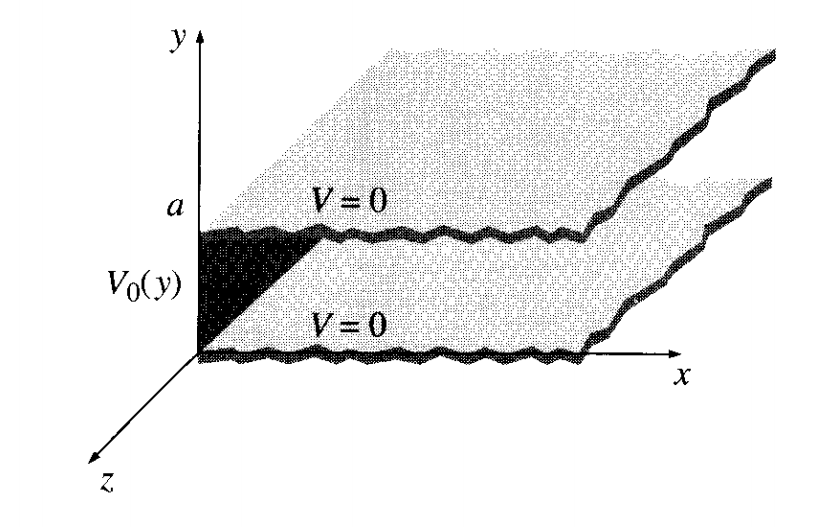
\includegraphics[width=0.6\textwidth]{ejemplo3-3-griffiths.png}
    \caption{Ejercicio \ref{ej:griffiths}. (Figura tomada de \cite{Griffiths}; a reemplazar por un esquema propio.)}
    \label{fig:griffiths}
\end{figure}
\end{ejer}



\part{Ecuaciones en derivadas parciales}
\chapter{Introducción}\label{cap:intro-III}

Hasta ahora, en el curso hemos estudiado distintos modelos de evolución temporal basados en ecuaciones diferenciales ordinarias, sistemas dinámicos y modelos continuos sencillos. En todos esos casos, el estado del sistema se describe mediante un número finito de variables que dependen del tiempo.

Las \emph{ecuaciones en derivadas parciales} (EDPs) aparecen cuando el estado del sistema depende de variables continuas adicionales, típicamente el espacio y el tiempo. En lugar de describir la evolución de unos pocos números, las EDPs gobiernan la evolución de funciones:
$$
u = u(x,t), \qquad u = u(x,y,t), \quad \text{o más generalmente } u = u(\xx,t).
$$
Desde el punto de vista del modelado continuo, las EDPs constituyen el lenguaje natural para describir fenómenos distribuidos en el espacio, como la difusión de calor o de contaminantes, la propagación de ondas, la evolución de densidades y numerosos procesos de transporte.

\section{Dos problemas conductores}\label{sec:conductores-III}

En esta parte los problemas conductores se desarrollan principalmente en el laboratorio; en el texto los planteamos, y volvemos sobre ellos cada vez que la teoría permite decir algo nuevo.

\subsection*{La temperatura del suelo}\label{sec:conductor-suelo}

En la Parte II estudiamos la temperatura del aire, que oscila con un ciclo diario y uno anual. Esa temperatura es la que ``ve'' la superficie del suelo, y el calor se difunde desde allí hacia abajo. Las estaciones meteorológicas miden la temperatura del suelo a varias profundidades (típicamente $5$, $10$, $20$, $50$ y $100$ cm), y los registros muestran algo notable: a medida que se baja, la oscilación diaria se atenúa muy rápido (a medio metro ya casi no se nota), la oscilación anual se atenúa mucho más lentamente, y ambas llegan \emph{retrasadas}: el máximo diario a $20$ cm ocurre varias horas después que en la superficie, y el máximo anual a un metro de profundidad ocurre semanas después que en la superficie. A suficiente profundidad la temperatura es constante todo el año (es el principio de las bodegas y de los sótanos).

Las preguntas son:
\begin{enumerate}
\item ¿Qué ecuación describe la temperatura $u(x,t)$ a profundidad $x$ y tiempo $t$, y con qué condiciones de borde?
\item ¿Por qué el ciclo diario penetra menos que el anual? ¿Cuánto menos? ¿De qué depende la profundidad de penetración?
\item ¿Cuánto vale el retraso a cada profundidad?
\item Dadas mediciones a varias profundidades, ¿se puede estimar la difusividad térmica del suelo? ¿Y comprobar que el modelo es correcto?
\item ¿A qué profundidad hay que enterrar una cañería para que no se congele en invierno?
\end{enumerate}
El modelo es la ecuación del calor en el semieje $x>0$ con una condición de borde \emph{periódica en el tiempo} en $x=0$. Veremos que el estado al que converge la solución no es un equilibrio sino una oscilación, y que la teoría de convergencia al equilibrio del Capítulo \ref{ch:intro-heat} se aplica igual.

\figpendiente{Temperatura del suelo a varias profundidades}{Registro real (o simulado) de temperatura a $0$, $10$, $20$, $50$ y $100$ cm durante una semana y durante un año, mostrando la atenuación y el retraso de los ciclos.}

\subsection*{La cuerda vibrante}\label{sec:conductor-cuerda}

El segundo problema es el más antiguo de la física matemática: una cuerda tensa, fija en sus extremos, que se pulsa o se golpea (una guitarra, un piano). Las preguntas:
\begin{enumerate}
\item ¿Qué ecuación describe el desplazamiento $u(x,t)$ de la cuerda y por qué?
\item ¿A qué frecuencias vibra la cuerda? ¿Cómo dependen de su longitud, su tensión y su masa? (Esto es lo que afina un músico.)
\item ¿Por qué una misma nota suena distinto en una guitarra y en un piano, si la frecuencia fundamental es la misma? ¿Qué determina el \emph{timbre}?
\item Si grabamos el sonido de una cuerda y calculamos su espectro con las herramientas de la Parte II, ¿qué esperamos ver? ¿Y qué vemos en realidad? ¿Qué le falta al modelo?
\end{enumerate}
El modelo es la ecuación de ondas en un intervalo, y su solución por series de Fourier es una superposición de \emph{modos normales} con frecuencias múltiplos enteros de una fundamental. La comparación entre ese espectro ideal y el espectro medido de una cuerda real (que no es exactamente armónico, y cuyos armónicos decaen a distinta velocidad) es el tema del laboratorio.

\figpendiente{Espectro de una cuerda real}{Espectro de potencia de la grabación de una cuerda de guitarra pulsada, con las frecuencias $k f_1$ marcadas para comparar con la predicción del modelo.}

\section{EDPs y ciencias de datos}

Aunque las EDPs tienen su origen en la física y la ingeniería, hoy desempeñan un papel importante en muchos problemas vinculados a las ciencias de datos, tanto de manera explícita como implícita.

En primer lugar, muchos procesos sobre datos pueden interpretarse como dinámicas continuas. Por ejemplo, el suavizado de señales o datos ruidosos puede verse como la evolución de una función bajo una ecuación de difusión. De manera análoga, los procesos de difusión en grafos y los métodos espectrales admiten descripciones continuas en términos de ecuaciones tipo calor.

Por otro lado, las EDPs están estrechamente relacionadas con técnicas de regularización y aprendizaje. Muchos problemas de optimización variacional —frecuentes en interpolación, ajuste de datos y aprendizaje automático— conducen a ecuaciones elípticas como condición de optimalidad. En este sentido, las EDPs aparecen como el límite continuo de ciertos algoritmos de optimización y métodos de inferencia.

\section{Conexión con el análisis de Fourier}

Las ecuaciones en derivadas parciales lineales clásicas, como la ecuación del calor o la ecuación de ondas, se comprenden particularmente bien a través del análisis de Fourier. En el espacio de frecuencias, estas ecuaciones describen cómo cada modo espectral evoluciona de manera independiente en el tiempo, permitiendo interpretar la dinámica como un proceso de filtrado de frecuencias.

Desde esta perspectiva, una EDP puede entenderse como un operador que transforma datos, reforzando o atenuando ciertas escalas, de forma muy cercana a lo que ocurre en el procesamiento de señales y el análisis espectral de datos.

\section{EDPs, modelos y datos}

En el contexto actual de las ciencias de datos, también resulta relevante el problema inverso: a partir de observaciones o datos experimentales, se busca identificar o aprender el modelo continuo subyacente, que a menudo adopta la forma de una ecuación en derivadas parciales. Este enfoque da lugar a modelos híbridos que combinan información proveniente de los datos con principios de modelado físico o geométrico.

\section{Objetivos de parte del curso}

En esta parte del curso no se busca desarrollar una teoría exhaustiva de las ecuaciones en derivadas parciales, sino introducir sus ideas fundamentales desde una perspectiva de modelado. Nos concentraremos en:
\begin{itemize}
    \item comprender qué tipos de fenómenos describen las EDP,
    \item estudiar ecuaciones prototipo como la ecuación del calor, la ecuación de Laplace y la ecuación de ondas,
    \item interpretar cualitativamente sus soluciones y su comportamiento,
    \item y establecer conexiones con herramientas y conceptos habituales en las ciencias de datos.
\end{itemize}

El objetivo principal es incorporar a las ecuaciones en derivadas parciales como una herramienta conceptual más del modelado continuo, especialmente útil cuando se trabaja con datos distribuidos en el espacio y el tiempo.


\chapter{La ecuación de difusión}\label{ch:intro-heat}

La ecuación de difusión, también conocida como ecuación del calor, es uno de los modelos fundamentales del modelado continuo. Describe la evolución temporal de la temperatura —o, más generalmente, de una cantidad que se difunde— en un medio continuo. A pesar de su forma matemática simple, esta ecuación aparece en una enorme variedad de contextos: transferencia de calor, difusión de sustancias, propagación de probabilidades y suavizado de datos.

\section{El principio de conservación}

El punto de partida conceptual de este modelo es el principio de conservación de la energía. En palabras de Richard Feynman (ver \cite{Feynman}):

\begin{quote}
``Hay un hecho —o, si ustedes prefieren, una ley— que gobierna todos los fenómenos naturales conocidos hasta la fecha. No se conoce excepción a esta ley —es exacta hasta donde sabemos—. La ley se llama conservación de la energía. Establece que hay cierta cantidad que llamamos energía, que no cambia en los múltiples cambios que ocurren en la naturaleza. Esta es una idea muy abstracta, porque es un principio matemático; significa que hay una cantidad numérica que no cambia cuando algo ocurre.''

\hfill —R. Feynman
\end{quote}

Esta observación enfatiza que la energía no se introduce a partir de un mecanismo microscópico, sino como una magnitud que satisface una ley de balance. Esa idea será el punto de partida para la deducción de la ecuación del calor.

\subsection{Balance de energía en una región}

Consideremos una región fija $V \subset \mathbb{R}^n$. Denotemos por $Q(V,t)$ la cantidad total de energía térmica contenida en $V$ en el instante $t$. El principio de conservación establece que la variación temporal de $Q(V,t)$ se debe a dos mecanismos:

\begin{itemize}
    \item el flujo de energía a través de la frontera $\partial V$,
    \item la energía generada o absorbida dentro de $V$ (por ejemplo, debido a reacciones químicas).
\end{itemize}

En forma simbólica, esta ley de balance puede escribirse como
$$
\frac{d}{dt} Q(V,t) = -\Phi(\partial V,t) + F(V,t),
$$
donde $\Phi(\partial V,t)$ representa el flujo total saliente de energía a través de la frontera, y $F(V,t)$ la energía generada en el interior de la región por unidad de tiempo.

\subsection{Formulación en términos de densidades}

Para obtener una descripción local, suponemos que todas las cantidades anteriores admiten una representación en términos de densidades.

Sea:
\begin{itemize}
    \item $u(\xx, t)$ la densidad de energía térmica por unidad de volumen,
    \item $\mathbf{J}(\xx, t)$ el flujo de energía (energía por unidad de tiempo y de área),
    \item $f(\xx, t)$ la densidad de energía generada por unidad de volumen y por unidad de tiempo.
\end{itemize}

Entonces, las cantidades globales se escriben como
$$
Q(V,t) = \int_V u(\xx,t)\, d\xx,
$$
$$
\Phi(\partial V,t) = \int_{\partial V} \mathbf{J}(\xx,t)\cdot \n\, dS,
$$
$$
F(V,t) = \int_V f(\xx,t)\, d\xx,
$$
donde $\n$ denota la normal exterior a la frontera.

Sustituyendo estas expresiones en la ecuación de balance se obtiene
$$
\frac{d}{dt} \int_V u(\xx,t)\, d\xx = - \int_{\partial V} \mathbf{J}\cdot \n\, dS + \int_V f(\xx,t)\, d\xx.
$$

Aplicando el teorema de la divergencia al término de flujo, resulta
$$
\frac{d}{dt} \int_V u\, d\xx = - \int_V \nabla \cdot \mathbf{J}\, d\xx + \int_V f\, d\xx.
$$

Como la región $V$ es arbitraria, se obtiene la forma local de la ley de conservación, conocida como \emph{ecuación de continuidad}:
$$
\partial_t u + \nabla \cdot \mathbf{J} = f.
$$

Esta ecuación expresa que la variación local de la energía se debe a la divergencia del flujo y a la presencia de fuentes o sumideros en el interior del dominio.

\subsection{Difusión y ley de Fourier}

Para cerrar el modelo es necesario especificar la relación entre el flujo $\mathbf{J}$ y la densidad de energía $u$. En muchos procesos térmicos y difusivos, el flujo está gobernado por la ley de Fourier:
$$
\mathbf{J} = -D \nabla u,
$$
donde $D>0$ es el coeficiente de difusión.

En ausencia de fuentes internas ($f=0$), al sustituir esta relación en la ecuación de continuidad se obtiene
$$
\partial_t u = D \Delta u,
$$
que es la \emph{ecuación del calor} o \emph{ecuación de difusión}.

Este modelo describe cómo la energía térmica se redistribuye en el espacio, tendiendo a eliminar gradientes y a producir distribuciones cada vez más homogéneas con el paso del tiempo.

\subsection{Condición inicial y condiciones de contorno}\label{sec:contorno}

La ecuación de difusión describe la evolución temporal de la temperatura (o de una cantidad difusiva) en el interior de un dominio. Para que el modelo esté completamente determinado, no alcanza con especificar la ecuación diferencial: es necesario complementar el problema con información adicional.

\subsubsection*{Condición inicial}

Dado que la ecuación del calor describe una evolución en el tiempo, es necesario prescribir el estado inicial del sistema. Esto se hace especificando la distribución inicial de temperatura:
$$
u(\xx,0) = u_0(\xx), \qquad \xx \in \Omega,
$$
donde $\Omega$ es la región del espacio ocupada por el sistema. Esta condición inicial representa el estado térmico del sistema en el instante a partir del cual comienza la evolución.

\subsubsection*{Condiciones de contorno}

Cuando el dominio espacial $\Omega$ es una región acotada, la evolución de la temperatura en su interior está influenciada por lo que ocurre en la frontera $\partial \Omega$. Esta interacción se modela mediante condiciones de contorno, que expresan distintos mecanismos físicos de intercambio de energía con el entorno.

Las condiciones de contorno más habituales en el contexto de la ecuación del calor son las siguientes.

\paragraph{\underline{Condiciones de Dirichlet} (temperatura impuesta).}

En este caso se prescribe el valor de la temperatura en la frontera del dominio:
$$
u(\xx,t) = g(\xx,t), \qquad \xx \in \partial \Omega.
$$
Este tipo de condición modela situaciones en las que el sistema está en contacto con un reservorio térmico que mantiene la frontera a temperatura fija (por ejemplo, una pared en contacto con un baño térmico).

\paragraph{\underline{Condiciones de Neumann} (flujo impuesto).}

Aquí se prescribe el flujo térmico normal a la frontera:
$$
- k \nabla u(\xx,t)\cdot \n = h(\xx,t), \qquad \xx \in \partial \Omega,
$$
donde $\n$ es la normal exterior a la frontera y $k$ es la conductividad térmica. Este tipo de condición representa un intercambio de calor controlado, como una fuente o un aislante térmico. En particular, el caso $h=0$ corresponde a una frontera aislada, sin flujo de calor.

\paragraph{\underline{Condiciones de Robin o de radiación}}

Este tipo de condición combina las dos anteriores y modela procesos de intercambio de calor con el ambiente, como la radiación o la convección:
$$
- k \nabla u(\xx,t)\cdot \n = \alpha \bigl(u(\xx,t) - u_{\text{ext}}(\xx,t)\bigr), \qquad \xx \in \partial \Omega,
$$
donde $\alpha>0$ es un coeficiente de transferencia térmica y $u_{\text{ext}}$ representa la temperatura del medio externo.

Las condiciones de Robin interpolan entre los casos de Dirichlet y Neumann y permiten modelar de manera más realista el intercambio de energía entre el sistema y su entorno.

\medskip

La elección de las condiciones iniciales y de contorno es una parte esencial del proceso de modelado, ya que determina de manera decisiva el comportamiento de las soluciones y su interpretación física.

\section{Movimiento browniano, difusión y paseo al azar}

La ecuación de difusión no sólo surge como un modelo macroscópico basado en leyes de conservación, sino que también puede interpretarse como el resultado promedio de un comportamiento microscópico esencialmente aleatorio. Esta conexión fue establecida de manera fundamental por Albert Einstein en su estudio del movimiento browniano.

\subsection{Movimiento browniano}

El movimiento browniano se refiere al movimiento irregular y errático de partículas microscópicas suspendidas en un fluido, observado experimentalmente a comienzos del siglo XIX por Robert Brown en \cite{Brown}. Durante mucho tiempo, este fenómeno careció de una explicación teórica convincente. Ver Figura \ref{fig:Browniano} para observar una realización de una partícula que se mueve al azar.
\begin{figure}[ht]
\centering
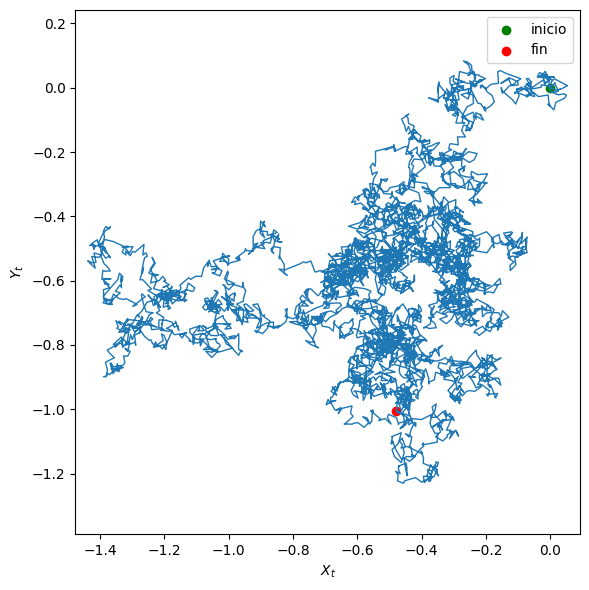
\includegraphics[width=0.5\textwidth]{Browniano.png}
\caption{Realización de una partícula en un movimiento Browniano.}
\label{fig:Browniano}
\end{figure}

En 1905, Albert Einstein proporcionó una descripción cuantitativa del movimiento browniano basada en la hipótesis de que las partículas visibles sufren una enorme cantidad de colisiones microscópicas con las moléculas del fluido. Estas colisiones, impredecibles a escala individual, producen un movimiento neto aleatorio que puede describirse estadísticamente.

En su artículo \cite{Einstein}, Einstein mostró que la evolución temporal de la densidad de probabilidad de encontrar una partícula browniana satisface la ecuación de difusión. Este resultado constituyó una de las primeras confirmaciones cuantitativas de la teoría molecular de la materia.

\subsection{Difusión como límite macroscópico}

Siguiendo a Einstein \cite{Einstein}, consideremos una gran cantidad de partículas idénticas que se mueven sobre una recta como resultado de un proceso microscópico aleatorio. En lugar de describir trayectorias individuales, nos concentramos en una descripción estadística.

Sea
$$
u(x, t)
$$
la densidad de partículas en la posición $x$ en el instante $t$, y sea
$$
\rho(y, \tau)
$$
la probabilidad de que una partícula se desplace una distancia $y$ durante un intervalo de tiempo $\tau$.

Suponemos que el proceso es homogéneo en el espacio y estacionario en el tiempo, de modo que la distribución de desplazamientos depende sólo de $y$ y de $\tau$, y no de la posición absoluta ni del instante inicial.

\medskip

La conservación del número total de partículas implica que la densidad en el instante $t+\tau$ puede obtenerse sumando las contribuciones de todas las partículas que, en el instante $t$, se encontraban en posiciones $x-y$ y se desplazaron una distancia $y$ durante el intervalo $\tau$. Esto conduce a la relación fundamental
$$
u(x,t+\tau) = \int_{\R} u(x-y, t)\,\rho(y, \tau)\,dy.
$$

Esta ecuación expresa que la densidad futura es el promedio, ponderado por la probabilidad de desplazamiento, de la densidad pasada.

\medskip

Suponemos ahora que los desplazamientos microscópicos son pequeños y simétricos. En particular, asumimos que $\rho$ satisface
$$
\int_\R \rho(y,\tau)\,dy = 1, \qquad \int_\R y\,\rho(y,\tau)\,dy = 0,
$$
y que el segundo momento es finito:
$$
\int_\R y^2\,\rho(y,\tau)\,dy = \sigma^2(\tau).
$$

Desarrollando $u(x-y,t)$ en serie de Taylor alrededor de $x$, se obtiene
$$
u(x-y,t) = u(x,t) - y\,\partial_x u(x,t) + \frac{y^2}{2}\,\partial_{xx} u(x,t) + \mathcal{O}(y^3).
$$

Sustituyendo este desarrollo en la ecuación integral y usando las propiedades de $\rho$, resulta
$$
u(x,t+\tau) = u(x,t) + \frac{\sigma^2(\tau)}{2}\,\partial_{xx} u(x,t) + \text{términos de orden superior}.
$$

Por otro lado, desarrollando el lado izquierdo en serie de Taylor respecto del tiempo,
$$
u(x,t+\tau) = u(x,t) + \tau\,\partial_t u(x,t) + \mathcal{O}(\tau^2).
$$

Comparando ambos desarrollos y despreciando términos de orden superior, se obtiene
$$
\partial_t u(x,t) = \frac{\sigma^2(\tau)}{2\,\tau}\,\partial_{xx} u(x,t).
$$

Definiendo el coeficiente de difusión como
$$
D = \frac{\sigma^2(\tau)}{2\,\tau},
$$
se llega finalmente a la ecuación de difusión
$$
\partial_t u = D\,\partial_{xx} u.
$$

\medskip

Este argumento muestra que la ecuación de difusión surge como una descripción macroscópica efectiva del movimiento aleatorio microscópico de las partículas. La dinámica determinista de la ecuación del calor aparece así como el límite continuo de un proceso fundamentalmente probabilístico.

\subsection{El paseo al azar y el paso al límite continuo}

Consideremos un modelo discreto del movimiento browniano en una dimensión. Dividimos el espacio en puntos igualmente espaciados
$$
x_j = j\,\Delta x, \qquad j \in \mathbb{Z},
$$
y el tiempo en instantes discretos
$$
t_n = n\,\Delta t, \qquad n \in \mathbb{N}.
$$

Sea $p_j^n$ la probabilidad de encontrar la partícula en el punto $x_j$ en el instante $t_n$. Supondremos que, en cada paso temporal, la partícula se desplaza una distancia $\Delta x$ hacia la derecha o hacia la izquierda con igual probabilidad $1/2$.

Bajo estas hipótesis, la evolución del paseo al azar está gobernada por la relación de recurrencia
$$
p_j^{\,n+1} = \frac{1}{2}\,p_{j-1}^{\,n} + \frac{1}{2}\,p_{j+1}^{\,n}.
$$

Esta ecuación expresa la conservación de la probabilidad: la probabilidad de estar en el sitio $j$ en el paso siguiente proviene de los sitios vecinos en el paso anterior.

Para conectar este modelo discreto con una descripción continua, introducimos una función $u(x,t)$ que representa una densidad de probabilidad en el espacio continuo. La relación entre $u$ y las probabilidades discretas se establece imponiendo que la probabilidad de encontrar la partícula en una celda espacial de tamaño $\Delta x$ alrededor de $x_j$ sea aproximadamente
$$
p_j^n \approx u(x_j,t_n)\,\Delta x.
$$

De manera equivalente, escribimos
$$
u(x_j,t_n) = \frac{p_j^n}{\Delta x}.
$$

Esta identificación asegura que la normalización de la probabilidad se preserve al pasar del modelo discreto al continuo:
$$
\sum_j p_j^n \approx \int_{\mathbb{R}} u(x,t_n)\,dx = 1.
$$


Sustituyendo $p_j^n = u(x_j,t_n)\,\Delta x$ en la relación de recurrencia se obtiene
$$
u(x_j,t_{n+1}) - u(x_j,t_n) = \frac{1}{2}\bigl[u(x_{j+1},t_n) - 2u(x_j,t_n) + u(x_{j-1},t_n)\bigr].
$$

Dividiendo ambos lados por $\Delta t$, resulta
$$
\frac{u(x_j,t_{n+1}) - u(x_j,t_n)}{\Delta t} = \frac{(\Delta x)^2}{2\,\Delta t} \, \frac{u(x_{j+1},t_n) - 2u(x_j,t_n) + u(x_{j-1},t_n)}{(\Delta x)^2}.
$$

El miembro izquierdo es una aproximación por diferencias finitas de la derivada temporal $\partial_t u$, mientras que el término de la derecha es una aproximación de la segunda derivada espacial $\partial_{xx} u$.


Tomando el límite $\Delta x \to 0$ y $\Delta t \to 0$ de manera que el cociente
$$
D = \frac{(\Delta x)^2}{2\,\Delta t}
$$
permanezca constante, se obtiene formalmente la ecuación de difusión
$$
\partial_t u = D\,\partial_{xx} u.
$$

Este procedimiento muestra cómo una ecuación diferencial parcial determinista surge como el límite continuo de un proceso aleatorio discreto. El coeficiente de difusión $D$ aparece como el parámetro que relaciona las escalas espaciales y temporales del paseo al azar.


\subsection{Paseo al azar asimétrico y ecuación de Fokker--Planck}

Consideramos un paseo al azar unidimensional definido sobre la red
$$
x_j = j\,\Delta x, \qquad t_n = n\,\Delta t.
$$
Denotamos por $p_j^n$ la probabilidad de encontrar la partícula en la posición $x_j$ al tiempo $t_n$.

A diferencia del paseo simétrico, suponemos ahora que las probabilidades de salto son distintas:
\begin{itemize}
  \item salto a la derecha con probabilidad $\alpha$,
  \item salto a la izquierda con probabilidad $\beta$,
\end{itemize}
con $\alpha+\beta=1$ y, en general, $\alpha\neq\beta$.

La ecuación de recurrencia para las probabilidades es entonces
\begin{equation}
p_j^{n+1} = \alpha\, p_{j-1}^n + \beta\, p_{j+1}^n.
\label{eq:rw_asim}
\end{equation}

Introducimos la densidad macroscópica $u(x,t)$ mediante la relación
$$
u(x_j,t_n) = \frac{p_j^n}{\Delta x},
$$
de modo que $u(x,t)\,dx$ representa la probabilidad de encontrar la partícula en un intervalo de longitud $dx$ alrededor de $x$.

Reescribiendo \eqref{eq:rw_asim} en términos de $u$, obtenemos
$$
u(x_j,t_{n+1}) = \alpha\,u(x_{j-1},t_n) + \beta\,u(x_{j+1},t_n).
$$

Desarrollando en series de Taylor alrededor del punto $(x_j,t_n)$,
\begin{align*}
u(x_j,t_{n+1}) &= u + \Delta t\,\partial_t u + o(\Delta t), \\
u(x_{j\pm1},t_n) &= u \pm \Delta x\,\partial_x u + \frac{(\Delta x)^2}{2}\,\partial_{xx}u + o((\Delta x)^2),
\end{align*}
y sustituyendo en la ecuación anterior, se obtiene
$$
\Delta t\,\partial_t u = (\beta-\alpha)\,\Delta x\,\partial_x u + \frac{(\Delta x)^2}{2}\,\partial_{xx}u + o(\Delta t,(\Delta x)^2).
$$

Dividiendo por $\Delta t$ y tomando el límite continuo $\Delta x,\Delta t\to0$, introducimos los parámetros macroscópicos
$$
v = \lim_{\Delta x,\Delta t\to0} \frac{(\alpha-\beta)\Delta x}{\Delta t}, \qquad D = \lim_{\Delta x,\Delta t\to0} \frac{(\Delta x)^2}{2\Delta t}.
$$

En este límite, la densidad $u(x,t)$ satisface la ecuación
\begin{equation}
\partial_t u = -v\,\partial_x u + D\,\partial_{xx}u,
\label{eq:fp_simple}
\end{equation}
que puede escribirse en forma conservativa como
$$
\partial_t u = -\partial_x(v\,u) + \partial_{xx}(D\,u).
$$

\subsubsection*{Interpretación de los coeficientes de deriva y difusión}

La ecuación de Fokker--Planck unidimensional
$$
\partial_t u = -v\,\partial_x u + D\,\partial_{xx} u
$$
describe la evolución temporal de la densidad de probabilidad $u(x,t)$ asociada a la posición de una partícula estocástica. Los coeficientes $v$ y $D$ admiten una interpretación directa en términos del movimiento microscópico subyacente.

\paragraph{Velocidad de deriva.}
El coeficiente $v$ representa la \emph{velocidad media de transporte} de la partícula. En el modelo de paseo al azar asimétrico, está dado por
$$
v = \lim_{\Delta t \to 0} \frac{\mathbb{E}[\Delta X]}{\Delta t} = \lim_{\Delta x,\Delta t\to 0} \frac{(\alpha-\beta)\Delta x}{\Delta t},
$$
donde $\mathbb{E}[\Delta X]$ es el desplazamiento medio en un intervalo de tiempo $\Delta t$. Un valor $v\neq 0$ indica la presencia de un sesgo sistemático en el movimiento, por ejemplo debido a una fuerza externa o a un gradiente del medio.

\paragraph{Coeficiente de difusión.}
El coeficiente $D$ mide la intensidad de las fluctuaciones aleatorias alrededor del movimiento medio. Más precisamente,
$$
D = \frac{1}{2}\lim_{\Delta t\to 0} \frac{\mathbb{E}\!\left[(\Delta X)^2\right]}{\Delta t},
$$
y está asociado al crecimiento lineal de la varianza $\mathrm{Var}[X(t)] = 2Dt$. En el paseo al azar discreto considerado,
$$
D = \lim_{\Delta x,\Delta t\to 0} \frac{(\Delta x)^2}{2\Delta t},
$$
independientemente del sesgo del movimiento.


La ecuación \eqref{eq:fp_simple} es un caso particular de la \emph{ecuación de Fokker--Planck}, introducida a comienzos del siglo XX en los trabajos de Fokker y Planck \cite{Fokker,Planck}.


%\chapter{La ecuación del calor y métodos de Fourier}
%
%En este capítulo estudiamos la ecuación del calor como modelo prototípico de difusión, y mostramos cómo puede resolverse explícitamente mediante herramientas de análisis espectral. En particular, presentamos dos enfoques complementarios: la separación de variables en dominios acotados y el uso de la transformada de Fourier en el espacio no acotado.

\section{La ecuación del calor en dimensión 1}\label{sec:heat.n=1}


Para empezar la discusión, nos centramos en el problema de difusión del calor en dimensión 1. Esto modela la difusión sobre una barra de longitud $L$ en donde las otras dimensiones pueden despreciarse. Entonces, la temperatura $u=u(x,t)$ debe satisfacer la ecuación
\begin{equation}
\partial_t u(x,t) = D\, \partial_{xx} u(x,t),\quad x\in [0,L],\ t>0.
\label{eq:heat}
\end{equation}

Como discutimos en el capítulo anterior, para poder resolver este problema, es necesario saber cómo era la distribución de temperatura al inicio del experimento y cómo es que la barra interactúa con el medio.

Consideremos que la barra está inicialmente a temperatura constante $u_0$. Se fija la temperatura en el extremo izquierdo a un valor constante $u_0$ y en el extremo derecho la temperatura es fijada un valor constante $u_L>u_0$. Luego, las condiciones iniciales y de contorno para $u$ resultan
\begin{equation}
u(x, 0) = u_0,\quad u(0,t)=u_0,\quad u(L, t)= u_L.
\label{eq:cond-contorno}
\end{equation}
Queremos saber cómo va a evolucionar la temperatura dentro de la barra.

Antes de realizar algún tipo de cálculo, tratemos de conjeturar qué es lo que sucede. Como $u_L>u_0$ el flujo de temperatura debe moverse del extremo derecho hacia el izquierdo. Por otro lado, el aumento de la temperatura interior producto del flujo debe compensarse con un flujo saliente del lado izquierdo que a la larga debe balancearse hasta que se llegue a un estado estacionario. Es interesante poder estimar el tiempo que se demora en llegar a ese estado estacionario.

Veamos que un análisis matemático riguroso de las ecuaciones \eqref{eq:heat}-\eqref{eq:cond-contorno} muestra exactamente ese comportamiento para la solución del problema.

Resulta conveniente empezar adimensionalizando el problema. Consideremos la variable adimensional
$$
y=\frac{x}{L}.
$$
Para adimensionalizar el tiempo, hacemos la siguiente observación. La constante de difusión $D$ tiene unidades de $m^2/s$, luego, la constante $\tau=L^2/D$ nos da una escala temporal característica para el problema de difusión. Esto sugiere introducir el tiempo adimensional como
$$
s = \frac{t}{\tau}.
$$
Finalmente, introducimos la temperatura adimensional
$$
v(y,s) = \frac{u(Ly, \tau s)-u_0}{u_L-u_0},
$$
que verifica:
\begin{align*}
v(y, 0) &= \frac{u(Ly, 0)-u_0}{u_L-u_0} = 0,\quad 0<y<1\\
v(0,s) & = \frac{u(0, \tau s)-u_0}{u_L-u_0} = 0,\quad v(1,s) = \frac{u(L, \tau s)-u_0}{u_L-u_0} = 1.
\end{align*}
Más aún,
$$
v_s - v_{yy} = \frac{1}{u_L-u_0}(\tau u_t(Ly, \tau s) - L^2 u_{xx}(Ly, \tau s)).
$$
Si recordamos que $\tau=L^2/D$, esta ecuación junto con \eqref{eq:heat} implica que
$$
v_s - v_{yy} = 0.
$$
Resumiendo, la temperatura adimensional $v$ en sus variables adimensionales $y, s$ verifica
\begin{equation}\label{eq:heat-adim}
\begin{cases}
v_s - v_{yy} = 0 & 0<y<1,\ s>0\\
v(0,s) = 0,\ v(1,s)=1\\
v(y, 0)=0
\end{cases}
\end{equation}

\subsection*{La solución estacionaria} 
Para resolver la ecuación \eqref{eq:heat-adim} resulta conveniente primero resolver el problema estacionario asociado. Esto es, buscamos una solución de la ecuación que no dependa de la variable temporal $s$. Esta función $v^*=v^*(y)$ debe satisfacer
$$
\begin{cases}
 v^*_{yy} = 0 & 0<y<1,\ s>0\\
v^*(0) = 0,\ v^*(1)=1,
\end{cases}
$$
es decir, $v^*(y) = y$. En términos de las variables originales, tenemos que la solución estacionaria es
$$
u^*(x) = u_0 + (u_L-u_0)\frac{x}{L}
$$
que corresponde a una distribución uniforme del flujo de calor a lo largo de la barra dado por la ley de Fourier
$$
\text{flujo} = -D\, u_x = -D\,\frac{u_L-u_0}{L}.
$$

\subsection*{El régimen transitorio}

Una vez que se conoce la solución estacionaria $v^*$, resulta conveniente introducir la función
$$
V(y, s) = v^*(y) - v(y, s) = y - v(y, s).
$$
Como esperamos que la solución $v(y, s)$ eventualmente alcance el estado estacionario, la función $V(y, s)$ representa el {\em régimen transitorio} que debe converger a cero cuando $s\to\infty$. Más aún, la tasa a la cual $V$ converge a cero nos da información de qué tan rápido la temperatura alcanza su distribución de equilibrio. La función $V$ satisface
\begin{align}\label{eq-transitorio}
&V_s - V_{yy} = 0,\qquad  0<y<1,\ s>0\\
\label{borde-transitorio}
&V(0,s) = 0,\ V(1,s)=0,\\
\label{inicial-transitorio}
&V(y, 0)=y.
\end{align}

\subsection*{Separación de variables}

Para hallar soluciones no triviales de \eqref{eq-transitorio}, buscamos soluciones especiales de la forma
$$
V(y, s) = w(y)z(s),
$$
con $w(0)=w(1)=0$. Sustituimos en \eqref{eq-transitorio} y obtenemos
$$
0 = V_s - V_{yy} = w(y)z'(s) - w''(y)z(s)
$$
y, reorganizando los términos,
$$
\frac{z'(s)}{z(s)} = \frac{w''(y)}{w(y)}.
$$
Como el lado izquierdo es una función de $s$ y el lado derecho es una función de $y$, la única posibilidad es que ambas expresiones sean constantes, digamos $\lambda\in\R$.

Luego, la función $w$ debe verificar:
\begin{equation}\label{autovw}
w''(y)-\lambda w(y) = 0,\quad w(0)=w(1)=0.
\end{equation}
Existen tres posibilidades para $\lambda$.
\subsubsection*{Caso 1: $\lambda=0$} En este caso, $w(y)=Ay+B$, pero las condiciones de contorno implican que $A=B=0$.

\subsubsection*{Caso 2: $\lambda=\mu^2>0$} En este caso
$$
w(y) = A e^{\mu y} + B e^{-\mu y}
$$
y nuevamente, las condiciones de contorno implican que $A=B=0$.

\subsubsection*{Caso 3: $\lambda=-\mu^2<0$}
En este caso
$$
w(y) = A\sin\mu y +  B\cos\mu y.
$$
Como $w(0)=0$ se tiene que $B=0$. Y de $w(1)=0$ obtenemos
$$
A\sin\mu = 0,
$$
de donde $A=0$ (solución trivial) o $\mu = k\pi$ con $k\in\N$.


Luego, las únicas soluciones no triviales de \eqref{autovw} son de la forma
$$
w_k(y) = A\sin k\pi y.
$$


Para estos valores de $\lambda_k = \pi^2 k^2$, podemos resolver para $z(s)$,
$$
z'(s) = -\lambda_k z(s),\Rightarrow z(s) = C e^{-\lambda_k s} = Ce^{-k^2\pi^2 s}.
$$

En conclusión, las soluciones fundamentales de \eqref{eq-transitorio}-\eqref{borde-transitorio} son
$$
V_k(y, s) = A_k e^{-k^2\pi^2 s}\sin(k\pi y).
$$

Observemos que  \eqref{eq-transitorio}-\eqref{borde-transitorio} es lineal, es decir que cualquier combinación lineal de las funciones $\{V_k(y, s)\}_{k\in\N}$ también va a resolver esas ecuaciones. Entonces para poder conseguir una solución de  \eqref{eq-transitorio}-\eqref{borde-transitorio} que además verifique la condición inicial \eqref{inicial-transitorio}, la buscamos en la forma
$$
V(y, s) = \sum_{k=1}^\infty A_k e^{-k^2\pi^2 s}\sin(k\pi y).
$$
Los coeficientes $A_k$ se calculan de forma tal que
\begin{equation}\label{V-inicial}
V(y, 0) = \sum_{k=1}^\infty A_k \sin(k\pi y) = y,\quad \text{para } 0<y<1.
\end{equation}

Como estamos buscando expandir a la función $f(y)=y$ como una serie de senos, resulta natural extender $f$ al intervalo $[-1,1]$ por imparidad (en este caso es simplemente extender $f(y)=y$ al intervalo $[-1,1]$). Como la función es real, su expansión resulta
$$
A_k = \int_{-1}^1 f(y)\sin(k\pi y)\, dy = 2\int_0^1 y\sin(k\pi y)\, dy = \frac{2(-1)^{k+1}}{k\pi},
$$
de donde 
\begin{equation}\label{eq:V}
V(y, s) = \sum_{k=1}^\infty \frac{2(-1)^{k+1}}{k\pi} e^{-k^2\pi^2 s}\sin(k\pi y).
\end{equation}
Ver la Figura \ref{fig:V-heat} para observar la evolución temporal de $V$.
\begin{figure}[ht]
\centering
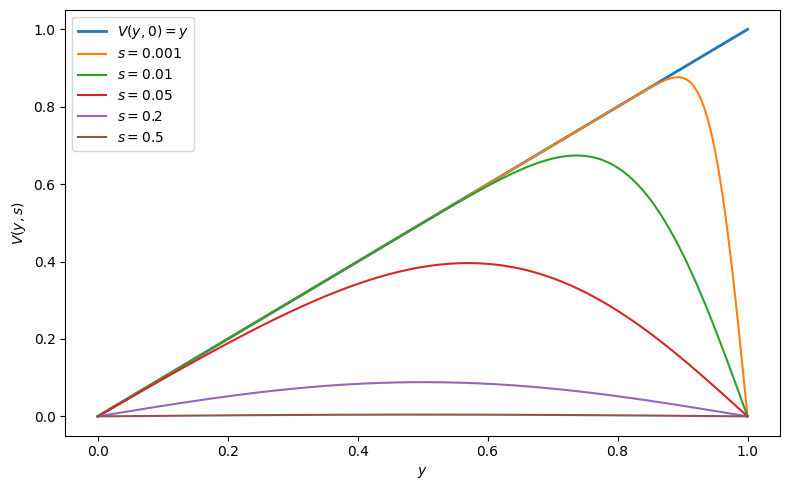
\includegraphics[width=0.6\textwidth]{V-heat.png}
\caption{Evolución temporal del régimen transitorio $V$.}
\label{fig:V-heat}
\end{figure}

\subsection*{Análisis del régimen transitorio}
Usando los resultados del Capítulo \ref{chap:conv.Fourier} (Teoremas \ref{teo.Dini} y \ref{teo.L2}), tenemos que la igualdad \eqref{V-inicial} se verifica puntualmente en todo $y\in [0, 1)$ y en sentido de media cuadrática, i.e.
$$
\lim_{N\to\infty} \int_0^1 \left|y-\sum_{k=1}^N \frac{2(-1)^{k+1}}{k\pi} \sin(k\pi y)\right|^2\, dy = 0.
$$

Veamos ahora que efectivamente \eqref{eq:V} define una función que es regular en el dominio $[0,1]\times(0, \infty)$, que verifica \eqref{eq-transitorio}-\eqref{borde-transitorio} y que alcanza la condición inicial \eqref{inicial-transitorio} cuando $s\downarrow 0$.

Para esto usaremos el siguiente resultado:
\begin{lema}\label{conv.f'}
Sean $f_k\colon [a, b]\to\R$, $k\in\N$, funciones de clase $C^1$ y sean $f, g\colon [a, b]\to\R$ continuas tales que
$$
f_k(x)\to f(x) \text{ para todo }x\in[a,b] \quad \text{y}\quad f_k'\rightrightarrows g \text{ uniformemente en } [a, b].
$$
Entonces $f$ es de clase $C^1$ y $g=f'$.
\end{lema}

\begin{proof}
Como $f_k$ es de clase $C^1$, podemos usar el Teorema Fundamental del Cálculo y escribir
$$
f_k(x) = f_k(a) + \int_a^x f'_k(y)\, dy,\quad x\in [a, b].
$$
Como $f_k'\rightrightarrows g$ y $f_k\to f$, podemos pasar al límite ($k\to\infty$) y obtenemos
$$
f(x) = f(a) + \int_a^x g(y)\, dy,
$$
de donde se concluye lo deseado.
\end{proof}

\begin{cor}\label{coro-reg}
Sean $f_k\colon[a, b]\to \R$, $k\in\N$, funciones de clase $C^1$ tales que $|f_k(x)|\le M_k$ y $|f'_k(x)|\le N_k$ con $\sum_{k=1}^\infty (M_k + N_k) < \infty$. Entonces la función
$$
f(x) = \sum_{k=1}^\infty f_k(x)
$$
es de clase $C^1$ en $[a, b]$ y 
$$
f'(x) = \sum_{k=1}^\infty f_k'(x).
$$
Es decir, la derivada de la serie se calcula derivando término a término la serie.
\end{cor}

\begin{proof}
La demostración es una combinación del criterio $M$ de Weierstrass (Teorema \ref{MdeW}) y del Lema \ref{conv.f'}. En efecto, para cada $N\in\N$ definimos
$$
S_N(x) = \sum_{k=1}^N f_k(x),
$$
entonces $S_N$ es de clase $C^1$,
$$
S_N'(x) = \sum_{k=1}^N f'_k(x)
$$
y, por el criterio $M$ de Weierstrass tenemos que
$$
S_N\rightrightarrows f\qquad \text{y}\qquad S_N'\rightrightarrows g,
$$
donde
$$
g(x) = \sum_{k=1}^\infty f_k'(x)
$$
Usamos ahora el Lema \ref{conv.f'} y se concluye lo deseado.
\end{proof}

Volviendo a la fórmula \eqref{eq:V}, usando el Corolario \ref{coro-reg}, debemos ver que si 
$$
V_k(y, s) = \frac{2(-1)^{k+1}}{k\pi} e^{-k^2\pi^2 s}\sin(k\pi y),
$$
entonces existen $M_k^{(0)}$, $M_k^{(1)}$, $M_k^{(2)}$ y $M_k^{(3)}$ tales que
$$
|V_k(y,s)|\le M_k^{(0)},\quad |\partial_y V_k(y,s)|\le M_k^{(1)},\quad |\partial_{yy} V_k(y,s)|\le M_k^{(2)},\quad |\partial_s V_k(y,s)|\le M_k^{(3)}
$$
y
$$
\sum_{k=1}^\infty M_k^{(i)}<\infty,\quad i=0,1,2,3.
$$
Es fácil ver que si $y\in [0,1]$ y $s\in [\delta, \infty)$ entonces
$$
M_k^{(i)}\le 2k\pi e^{-k^2\pi^2\delta},\quad i=0,1,2,3
$$
y como
$$
\sum_{k=1}^\infty ke^{-ak^2} < \infty, \quad \text{para } a>0,
$$
obtenemos que $V(y, s)$ es de clase $C^{2,1}$ (i.e. dos veces diferenciable en $y$ y diferenciable en $s$ con derivadas continuas) y sus derivadas se calculan derivando término a término la serie, de donde
$$
\partial_s V - \partial_{yy} V = 0 \quad \text{en } [0,1]\times [\delta, \infty),
$$
para todo $\delta>0$, luego satisface \eqref{eq-transitorio}.

Como $V$ resulta continua para $y\in [0,1]$ podemos evaluar \eqref{eq:V} en $y=0$ y en $y=1$ y obtenemos \eqref{borde-transitorio}.

Veamos que $V$ satisface \eqref{inicial-transitorio}. Haremos la cuenta en media cuadrática, y queda de ejercicio al lector verificar que $V(y,s)\to y$ cuando $s\downarrow 0$ puntualmente para $y\in [0, 1)$.

Usando la identidad de Plancherel, Corolario \ref{plancherel}, tenemos que
$$
\int_0^1 |y - V(y,s)|^2\, dy = \frac{4}{\pi^2} \sum_{k=1}^\infty \frac{\left(e^{-k^2\pi^2 s} - 1\right)^2}{k^2}.
$$
Observemos que, para $s>0$, 
$$
\frac{\left(e^{-k^2\pi^2 s} - 1\right)^2}{k^2}\le \frac{1}{k^2}
$$
y como la serie $\sum_{k=1}^\infty 1/k^2$ converge, podemos pasar al límite en la sumatoria obteniendo
$$
\int_0^1 |y - V(y,s)|^2\, dy\to 0 \quad \text{cuando }s\downarrow 0.
$$

\subsection*{Unicidad del régimen transitorio}
Veamos que, efectivamente, $V$ es la única solución de \eqref{eq-transitorio}-\eqref{inicial-transitorio}. Supongamos que $W(y,s)$ es otra solución, entonces si llamamos $w(y, s) = V(y, s) - W(y, s)$ tenemos que $w$ verifica
$$
\begin{cases}
w_s - w_{yy} = 0 & \text{en } [0,1]\times (0,\infty)\\
w(0,s) = w(1,s)=0\\
w(y, 0)=0
\end{cases}
$$

Multiplicamos esta ecuación por $w$ e integramos en $[0,1]$ para $s>0$ y obtenemos
$$
\int_0^1 w w_s\, dy - \int_0^1 w w_{yy}\, dy = 0.
$$
Observemos que $w w_s = \frac12 (w^2)_s$, de donde
$$
\int_0^1 w w_s\, dy = \frac12\frac{d}{ds}\int_0^1 w^2\, dy.
$$

Ahora, usando la fórmula de integración por partes y observando que $w(0,s)=w(1,s)=0$,
$$
\int_0^1 w w_{yy}\, dy = - \int_0^1 (w_y)^2\, dy \le 0.
$$
Combinando estas estimaciones, llegamos a
$$
\frac12\frac{d}{ds}\int_0^1 w^2\, dy\le 0.
$$
Es decir que si llamamos
$$
e(s) = \int_0^1 w(y,s)^2\, dy,
$$
tenemos que $e(0)=0$, $e(s)\ge 0$ para $s\ge 0$ y $e'(s)\le 0$. Esto implica que $e(s)=0$ para todo $s$ y por ende $w=0$. Es decir $V=W$ como queríamos ver.

\subsection*{Vuelta a las variables originales}

En términos de las variables originales, la solución queda expresada como
$$
u(x, t) = u_0 + (u_L-u_0)\frac{x}{L} - (u_L-u_0)\sum_{k=1}^\infty (-1)^{k+1}\frac{2}{k\pi} e^{-\frac{k^2\pi^2 D}{L^2} t} \sin\frac{k\pi}{L}x.
$$
\begin{figure}[ht]
\centering
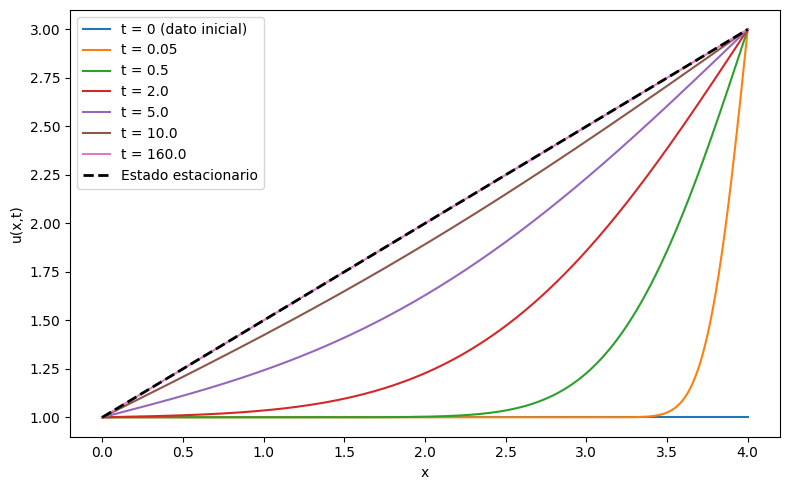
\includegraphics[width=0.6\textwidth]{u-heat.png}
\caption{Evolución temporal la solución $u(x,t)$ de \eqref{eq:heat}-\eqref{eq:cond-contorno}. En este ejemplo, $L=4$, $D=0.1$; entonces $L^2/D=160$.}
\label{fig:u-heat}
\end{figure}
En la Figura \ref{fig:u-heat} se puede ver la solución del problema original \eqref{eq:heat}-\eqref{eq:cond-contorno}. Observar como inmediatamente la solución toma los valores iniciales lo que genera una discontinuidad en $x=L$ para $t=0$. 

De la expresión obtenida para $u(x, t)$ se confirma nuestra suposición original sobre la evolución temporal de la temperatura hacia el estado estacionario. Efectivamente, cada uno de los términos de la sumatoria converge exponencialmente rápido a cero cuando $t\to\infty$ y $u(x, t) \to  u_0 + (u_L-u_0)\frac{x}{L}$ cuando $t\to\infty$.

Adicionalmente, observemos que entre los términos de la serie, el primero (que corresponde a $k=1$) decae mucho más lento que los otros e inmediatamente determina el desvío de $u$ con el equilibrio y este desvío es {\em independiente de la condición inicial}. Este término principal corresponde a una sinusoide amortiguada
$$
\frac{2}{\pi}e^{-\frac{\pi^2 D}{L^2}t} \sin\frac{\pi}{L}x.
$$
Observemos que en este modo, la concentración del calor ocurre en $x=L/2$, donde la temperatura alcanza su amplitud máxima de $\tfrac{2}{\pi}\exp(-\tfrac{\pi^2 D}{L^2}t)$. A tiempo $t=L^2/D$, la amplitud decae a $\tfrac{2}{\pi}\exp(-\pi^2)\simeq 3.3\times 10^{-5}$. Este cálculo sencillo nos indica que se necesita un tiempo aproximado de $L^2/D$ para llegar al estado estacionario. Observar la figura \eqref{fig:u-heat} donde se ve que a ese tiempo característico la solución es indistinguible del estado estacionario.

\section{La ecuación del calor en la recta}

La ecuación del calor en la recta real $\R$ viene dada por
\begin{equation}\label{heat-R}
\begin{cases}
u_t - D u_{xx} = 0, & x\in\R,\ t>0,\\
u(x,0) = g(x).
\end{cases}
\end{equation}

Cuando se quiere resolver la ecuación del calor en toda la recta real $\R$, el método utilizado en la sección anterior ya no es suficiente. Como vimos allí, al trabajar en la recta no es posible descomponer una función como una suma de un conjunto discreto de frecuencias (series de Fourier); en su lugar, la herramienta natural es la transformada de Fourier.

En la Proposición~\ref{prop.analiticas} vimos que la transformada de Fourier posee la propiedad de transformar derivadas en el espacio físico en productos en el espacio de frecuencias. Esta propiedad permite, como veremos a continuación, reducir el problema de resolver una ecuación en derivadas parciales para $u$ a resolver una ecuación diferencial ordinaria para su transformada $\hat u$.

En efecto, si aplicamos la transformada de Fourier a la ecuación~\eqref{heat-R} y usamos la linealidad de la transformada, obtenemos
\[
\widehat{u_t} - D\,\widehat{u_{xx}} = 0.
\]
Usando la Propiedad~2 de la Proposición~\ref{prop.analiticas}, se tiene
\[
\widehat{u_{xx}}(\xi) = -4\pi^2\xi^2\,\hat u(\xi).
\]
Por otro lado,
\[
\widehat{u_t}(\xi)
= \int_{-\infty}^{\infty} u_t(x,t)\,e^{-2\pi i x\xi}\,dx
= \frac{d}{dt}\int_{-\infty}^{\infty} u(x,t)\,e^{-2\pi i x\xi}\,dx
= \frac{d}{dt}\hat u(\xi,t),
\]
donde hemos intercambiado derivación e integración, lo cual es válido bajo hipótesis razonables de regularidad.

Por lo tanto, la función $\hat u=\hat u(\xi,t)$ satisface la ecuación
\[
\frac{d}{dt}\hat u(\xi,t) + 4\pi^2 D\xi^2\,\hat u(\xi,t) = 0.
\]
Fijando $\xi$ y definiendo $v(t)=\hat u(\xi,t)$, obtenemos la ecuación diferencial ordinaria
\[
v'(t) + 4\pi^2 D\xi^2\,v(t) = 0.
\]
Se trata de una ecuación lineal de primer orden con coeficientes constantes, cuya solución general es
\[
v(t) = C\,e^{-4\pi^2 D\xi^2\,t}.
\]

Para determinar la constante $C$, observamos que
\[
C = v(0) = \hat u(\xi,0)
= \int_{-\infty}^{\infty} u(x,0)\,e^{-2\pi i x\xi}\,dx
= \int_{-\infty}^{\infty} g(x)\,e^{-2\pi i x\xi}\,dx
= \hat g(\xi).
\]
Concluimos entonces que
\begin{equation}\label{hatheat}
\hat u(\xi,t) = \hat g(\xi)\,e^{-4\pi^2 D\xi^2\,t}.
\end{equation}

Esta expresión muestra que, en el espacio de frecuencias, la solución de la ecuación del calor en $\R$ hace decaer exponencialmente las frecuencias del dato inicial: cuanto mayor es la frecuencia, más rápido es su decaimiento. La ecuación del calor es un \emph{filtro pasabajos} que se vuelve cada vez más severo con el tiempo.

\begin{obs}[Irreversibilidad]
La misma fórmula muestra por qué la ecuación del calor \emph{no se puede correr hacia atrás}. Si quisiéramos recuperar el dato $g$ a partir de la solución en un tiempo $t>0$, tendríamos que multiplicar $\hat u(\xi,t)$ por $e^{4\pi^2D\xi^2t}$, que amplifica sin límite las frecuencias altas: un error de medición arbitrariamente chico en $u(\cdot,t)$, si contiene frecuencias altas, se traduce en un error arbitrariamente grande en $g$. El problema de reconstruir el pasado de un proceso difusivo (o de ``desenfocar'' una imagen que fue suavizada) está \emph{mal planteado}, y sólo puede tratarse con información adicional sobre la solución buscada (regularización). Este tipo de problemas inversos es central en ciencia de datos.
\end{obs}

La fórmula~\eqref{hatheat}, sin embargo, no es completamente satisfactoria, ya que lo que deseamos es una expresión explícita para $u(x,t)$.

Para ello, recordamos que, usando el Ejemplo~\ref{ej:gaussiana} y el ítem~5 de la Proposición~\ref{prop.algebraica}, se tiene
\[
e^{-4\pi^2 D\xi^2\,t}
= \mathcal F\!\left[\frac{1}{\sqrt{4\pi Dt}}
e^{-\frac{x^2}{4Dt}}\right](\xi).
\]
Aplicando entonces el Teorema~\ref{trans.conv}, obtenemos
\[
\hat u(\xi,t)
= \widehat{(g*\Phi)(\cdot,t)}(\xi),
\]
donde
\[
\Phi(x,t) = \frac{1}{\sqrt{4\pi Dt}}\,e^{-\frac{x^2}{4Dt}}.
\]

En consecuencia,
\[
u(x,t)
= (g*\Phi)(x,t)
= \int_{-\infty}^{\infty} g(y)\,\Phi(x-y,t)\,dy
= \frac{1}{\sqrt{4\pi Dt}}
\int_{-\infty}^{\infty} g(y)\,e^{-\frac{(x-y)^2}{4Dt}}\,dy.
\]

\begin{obs}
La función
\[
\Phi(x,t)=\frac{1}{\sqrt{4\pi Dt}}\,e^{-\frac{x^2}{4Dt}}
\]
coincide con la densidad de una distribución normal centrada en $0$, de varianza $2Dt$. En consecuencia, la solución
\[
u(x,t)=(g*\Phi)(x,t)
\]
puede interpretarse como un promedio ponderado del dato inicial $g$, donde los valores de $g$ cercanos a $x$ tienen mayor peso, y la ponderación viene dada por una distribución gaussiana.

A medida que $t$ crece, la varianza de esta distribución aumenta (ver Figura \ref{fig:sol-fundamental}), lo que implica que el promedio se realiza sobre regiones cada vez más amplias del espacio. Desde este punto de vista, la ecuación del calor actúa como un mecanismo de suavizado que difunde la información inicial, eliminando gradualmente las oscilaciones finas y haciendo que la solución se vuelva cada vez más regular.
\end{obs}
\begin{figure}[ht]
\centering
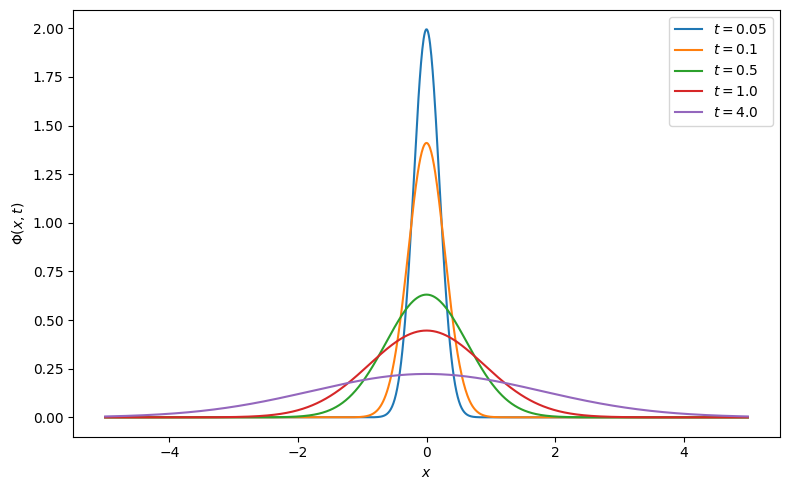
\includegraphics[width=0.5\textwidth]{sol-fundamental.png}
\caption{Distribución $\Phi(x,t)$ para distintos valores de $t$.}
\label{fig:sol-fundamental}
\end{figure}

\subsection*{Conservación de la masa}

Una propiedad fundamental de la ecuación del calor en la recta es la conservación de la masa total. Más precisamente, si $u$ es la solución de \eqref{heat-R} asociada al dato inicial $g$, entonces
\[
\int_{\R} u(x,t)\,dx = \int_{\R} g(x)\,dx \qquad \text{para todo } t>0.
\]

En efecto, usando la representación explícita de la solución como convolución con el núcleo del calor, obtenemos
\[
\int_{\R} u(x,t)\,dx
= \int_{\R} \int_{\R} g(y)\,\Phi(x-y,t)\,dy\,dx.
\]
Intercambiando el orden de integración y usando que $\Phi(\cdot,t)$ es una densidad de probabilidad, es decir,
\[
\int_{\R} \Phi(x-y,t)\,dx = 1,
\]
se concluye que
\[
\int_{\R} u(x,t)\,dx
= \int_{\R} g(y)\left( \int_{\R} \Phi(x-y,t)\,dx \right)dy
= \int_{\R} g(y)\,dy.
\]

Este resultado muestra que, si bien la ecuación del calor difunde y suaviza el dato inicial, redistribuyendo la masa en el espacio, la cantidad total de calor permanece constante a lo largo del tiempo.


\section{La ecuación del calor en dimensión \texorpdfstring{$n>1$}{n>1}}

Como vimos en el Capítulo \ref{ch:intro-heat}, el problema de difusión en dimensión $n>1$ está gobernado por la ecuación del calor
\begin{equation}\label{eq:u}
\begin{cases}
u_t = D\Delta u + f & \text{en } Q_T\\
u(\xx, 0) = g(\xx) & \text{en } \overline{\Omega}\\
\text{+ condiciones de contorno} & \text{en } \partial\Omega\times(0,T]
\end{cases}
\end{equation}
donde $\Omega\subset \R^n$, $T>0$, $Q_T = \Omega\times(0, T)$. Ver Figura \ref{fig:QT}.
\begin{figure}[ht]
\centering
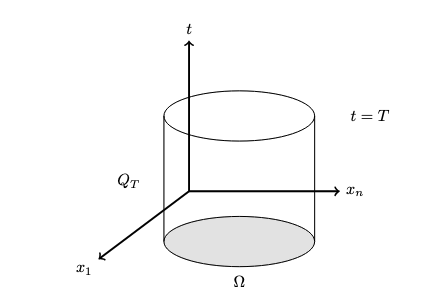
\includegraphics[width=0.5\textwidth]{QT.png}
\caption{Cilindro espacio-temporal $Q_T=\Omega\times(0,T)$.}
\label{fig:QT}
\end{figure}
Las condiciones de contorno fueron discutidas en la sección \ref{sec:contorno} y pueden ser
\begin{itemize}
\item Dirichlet:
$$
u = h,
$$
\item Neumann:
$$
\partial_\n u = \nabla u\cdot \n = h,\quad \text{($\n$ es la normal exterior unitaria a $\Omega$)}
$$
\item Robin o radiación: 
$$
\partial_\n u + \alpha u = h \quad (\alpha>0),
$$
\item mixtas:
$$
u=h_1\text{ en }\partial_D\Omega,\quad \partial_\n u = h_2\text{ en }\partial_N\Omega
$$
donde $\partial\Omega = \partial_D\Omega\cup\partial_N\Omega$ es una partición de la frontera.
\end{itemize}

\subsection{Unicidad}\label{sec:unicidad}
Veamos que usando métodos similares a como probamos la unicidad del régimen transitorio en la sección anterior, podemos probar unicidad de soluciones para \eqref{eq:u}.

Efectivamente, supongamos que $u_1$ y $u_2$ son dos soluciones de \eqref{eq:u} y llamemos $w=u_1-u_2$. Entonces, $w$ satisface
\begin{equation}\label{eq:w}
\begin{cases}
w_t = D\Delta w & \text{en } Q_T\\
w(\xx, 0) = 0 & \text{en } \overline{\Omega}\\
\text{+ condiciones de contorno homogéneas} & \text{en } \partial\Omega\times(0,T]
\end{cases}
\end{equation}
es decir, $w$ va a verificar el mismo tipo de condiciones de contorno que $u_1, u_2$ pero con $h=0$.

Multiplicamos la ecuación por $w$ e integramos para obtener
\begin{equation}\label{test.w}
\int_\Omega w w_t\, d\xx = D\int_\Omega w \Delta w\, d\xx.
\end{equation}
Al igual que antes, observamos que
$$
\int_\Omega w w_t\, d\xx = \frac12\frac{d}{dt}\int_\Omega w^2\, d\xx.
$$
Para tratar el otro término, debemos usar la {\em fórmula de integración por partes} en $\R^n$. Esta fórmula es una consecuencia del {\em Teorema de la divergencia de Gauss}.
\begin{teo}[Teorema de la divergencia de Gauss]\label{Gauss}
Sea $F\colon \R^n \to\R^n$ un campo de clase $C^1$. Entonces
$$
\int_\Omega \div F\, d\xx = \int_{\partial\Omega} F\cdot\n\, dS,
$$
donde $\n$ es la normal exterior unitaria a la superficie $\partial\Omega$.
\end{teo}
Este teorema, en $\R^3$ se estudia en Análisis 2 y pueden repasar su demostración, por ejemplo, en \cite{Tromba}. Recordemos que si $F = (f_1,\dots,f_n)$, entonces
$$
\div F = \nabla \cdot F = \partial_{x_1}f_1 + \cdots + \partial_{x_n} f_n.
$$
Como un corolario inmediato de este resultado tenemos la siguiente fórmula de integración por partes,
\begin{teo}[Fórmula de integración por partes]\label{partes}
Sean $u\colon \R^n\to\R$  de clase $C^1$ y $v\colon \R^n\to\R$ de clase $C^2$. Entonces
$$
\int_\Omega u\Delta v\, d\xx = -\int_\Omega \nabla u\cdot\nabla v\, d\xx + \int_{\partial\Omega} u \nabla v\cdot\n\, dS.
$$
\end{teo}

\begin{proof}
La demostración es inmediata. En efecto, llamemos $F = u\nabla v$. Entonces $F$ es un campo vectorial de clase $C^1$ y
$$
\div F = \nabla u\cdot\nabla v + u\Delta v.
$$
Aplicando entonces el Teorema \ref{Gauss}, obtenemos
$$
\int_\Omega (\nabla u\cdot\nabla v + u\Delta v)\, d\xx = \int_\Omega \div F\, d\xx = \int_{\partial\Omega} F\cdot\n\, dS =  \int_{\partial\Omega} u \nabla v\cdot\n\, dS.
$$
Esto culmina la demostración.
\end{proof}

Apliquemos ahora el Teorema \ref{partes} para tratar el segundo término en \eqref{test.w}
$$
\int_\Omega w\Delta w\, d\xx = -\int_\Omega |\nabla w|^2\, d\xx + \int_{\partial\Omega} w\nabla w\cdot\n\, dS.
$$
La integral de superficie vale 0 si se consideran condiciones de Dirichlet, Neumann o mixtas. En el caso de las condiciones de Robin, se obtiene
$$
\int_{\partial\Omega} w\nabla w\cdot\n\, dS = -\alpha\int_{\partial\Omega} w^2\, dS\le 0.
$$
Es decir que en cualquiera de estas situaciones tenemos que
$$
\int_\Omega w\Delta w\, d\xx\le 0.
$$
En consecuencia, de \eqref{test.w} obtenemos que
$$
\frac{d}{dt}\int_\Omega w^2\, d\xx \le 0.
$$
Entonces, llamando
$$
E(t) = \int_\Omega w^2\, d\xx 
$$
tenemos que $E(0)=0$, $E(t)\ge 0$ y $E'(t)\le 0$. Todas estas condiciones implican que $E(t)=0$ para todo $t$ de donde se deduce que $w=0$ como queríamos ver.

\subsection{Principio del máximo}

El hecho de que el calor fluya desde regiones de mayor temperatura hacia regiones de menor temperatura implica que una solución de la ecuación del calor homogénea alcanza sus valores máximo y mínimo sobre el borde parabólico $\partial_p Q_T = \partial\Omega\times (0, T]\cup \overline\Omega\times\{0\}$. Este resultado se conoce como el {\em principio del máximo}.

Además, la ecuación refleja la {\em irreversibilidad temporal} de los fenómenos que describe, en el sentido de que el futuro no puede influir sobre el pasado (principio de causalidad). En otras palabras, el valor de una solución $u$ en el tiempo $t$ es independiente de cualquier cambio en los datos posterior a $t$.

El principio del máximo, formulado precisamente, dice lo siguiente:
\begin{teo}[Principio del máximo]\label{ppio.maximo}
Sea $\Omega\subset\R^n$ acotado y sea $u\in C^{2,1}(Q_T)\cap C(\overline{Q}_T)$ una función que verifica
$$
u_t - D\Delta u = f\le 0 \quad \text{en } Q_T.
$$
Entonces $u$ alcanza su máximo en $\partial_p Q_T$, i.e.
$$
\max_{\overline{Q}_T} u = \max_{\partial_p Q_T} u.
$$
En particular, si $u$ es negativa en $\partial_p Q_T$, entonces es negativa en todo $Q_T$.
\end{teo}

\begin{proof}
Supongamos primero que $f<0$ en $Q_T$.

Supongamos que existe $(x_0, t_0)\in Q_T$ tal que $u(x_0, t_0)=\max_{\overline{Q}_T} u$. Entonces, se tiene que
$$
u_{x_i}(x_0, t_0)=0\qquad\text{y}\qquad u_{x_i x_i}(x_0, t_0)\le 0,\qquad 1\le i\le n.
$$
Por otro lado, si $t_0<T$,
$$
u_t(x_0, t_0) = 0
$$
y si $t_0=T$,
$$
u_t(x_0, t_0)\ge 0.
$$
Juntando estas estimaciones, obtenemos que
$$
u_t(x_0, t_0) - D\Delta u(x_0, t_0) = \underbrace{u_t(x_0, t_0)}_{\ge 0} - D\sum_{i=1}^n \underbrace{u_{x_i x_i}(x_0, t_0)}_{\le 0} \ge 0,
$$
lo que contradice el hecho de que $f<0$. Luego, $\max_{\overline{Q}_T} u = \max_{\partial_p Q_T} u$ en este caso.

Veamos ahora el caso general en que $f\le 0$ en $Q_T$. 

Sea $\ve>0$ y definimos $u_\ve(x, t) = u(x, t)-\ve t$. Entonces, $u_\ve$ verifica
$$
(u_\ve)_t - D\Delta u_\ve = u_t - D\Delta u - \ve = f - \ve< 0.
$$
Luego, por el caso anterior,
$$
\max_{\overline{Q}_T} u_\ve = \max_{\partial_p Q_T} u_\ve.
$$
Como $u_\ve\rightrightarrows u$, el teorema sigue tomando límite cuando $\ve\to 0$.
\end{proof}

Tenemos los siguientes corolarios.

\begin{cor}
Sea $u\colon \R^n\times[0, \infty)\to\R$ tal que
$$
u_t - D\Delta u = 0\quad \text{en } Q_T.
$$
Entonces
$$
\min_{\partial_p Q_T} u \le u(\xx, t)\le \max_{\partial_p Q_T} u\quad \text{para todo }(\xx, t)\in Q_T.
$$
\end{cor}

\begin{proof}
Aplicar el Teorema \ref{ppio.maximo} a $u$ y $-u$. Los detalles quedan para el lector.
\end{proof}

\begin{cor}[Comparación y estabilidad]
Sean $u, v\colon \R^n\times[0,\infty)\to\R$ tales que
$$
u_t - D\Delta u = f_1\qquad \text{y}\qquad v_t - D\Delta v = f_2.
$$
Entonces
\begin{enumerate}
\item Comparación: Si $u\ge v$ en $\partial_p Q_T$ y $f_1\ge f_2$ en $Q_T$, entonces $u\ge v$ en $Q_T$.

\item Estabilidad: Tenemos la siguiente estimación
$$
\max_{\overline Q_T} |u-v|\le \max_{\partial_p Q_T} |u-v| + T\max_{\overline Q_T} |f_1 - f_2|.
$$
\end{enumerate}
\end{cor}

\begin{proof}
Los detalles quedan para el lector. Damos sólo unas breves sugerencias:
\begin{enumerate}
\item Aplicar el Teorema \ref{ppio.maximo} a la función $w=v-u$.

\item Considerar $w=v-u$, $M=\max_{\overline Q_T} |f_1 - f_2|$ y aplicar el Teorema \ref{ppio.maximo} a las funciones $z_{\pm} = \pm w - Mt$.
\end{enumerate}
\end{proof}

\subsection{Convergencia al equilibrio}\label{sec:convergencia.equilibrio}

Consideremos el problema de difusión
\begin{equation}\label{eq:heat-n}
\begin{cases}
u_t - D\Delta u = f(\xx) & \text{en } Q_T = \Omega\times (0,T)\\
u(\xx, 0) = g(\xx) & \text{en } \Omega\\
u(\xx, t) = h(\xx) & \text{en }\partial\Omega\times (0,T)
\end{cases}
\end{equation}

Para simplificar, asumimos que tanto la fuente $f$ como el dato de contorno $h$ son independientes del tiempo.

La pregunta que queremos responder es ¿qué sucede con la distribución de temperatura $u$ cuando $t\to\infty$?

El problema lo hemos estudiado en el caso de dimensión 1 y vimos que $u$ converge al estado estacionario $u^*$ que es la solución del problema
\begin{equation}\label{eq:est-n}
\begin{cases}
-D\Delta u^* = f & \text{en }\Omega\\
u^* = h & \text{en }\partial\Omega
\end{cases}
\end{equation}


Veamos que el mismo fenómeno se produce también en el caso $n$-dimensional. Para esto vamos a asumir que el problema \eqref{eq:est-n} admite una única solución. Este problema (llamado el problema de Poisson) será estudiado con detalle en el capítulo siguiente.

Para analizar este comportamiento, conviene introducir el \emph{régimen transitorio}, definido como la diferencia entre la solución $u$ de \eqref{eq:heat-n} y el estado estacionario $u^*$:
$$
v(\xx, t) = u(\xx, t)-u^*(\xx).
$$
Observemos que el régimen transitorio $v$ verifica
$$
\begin{cases}
v_t - D\Delta v = 0 & \text{en } Q_T\\
v = 0 & \text{en } \partial\Omega\times (0,T)\\
v(\xx, 0 ) = \bar g(\xx) & \text{en }\Omega,
\end{cases}
$$
donde $\bar g(\xx) = g(\xx)-u^*(\xx)$. Veamos que el régimen transitorio $v$ tiende a 0 independientemente del dato inicial $\bar g$.

Ahora, si llamamos
$$
E(t) = \frac12\int_\Omega v^2(\xx, t)\, d\xx,
$$
argumentando de manera análoga a lo hecho en la sección \ref{sec:unicidad}, tenemos que
\begin{equation}\label{energia1}
E'(t) + D\int_\Omega |\nabla v(\xx, t)|^2\, d\xx \le 0.
\end{equation}

En esta ocasión, queremos ir un paso más allá, no nos alcanza con la estimación trivial
$$
\int_\Omega |\nabla v(\xx, t)|^2\, d\xx\ge 0
$$
sino que queremos una estimación que relacione el tamaño de $v$ con el de su gradiente.

Esa estimación nos la da el siguiente resultado.
\begin{teo}[Desigualdad de Poincaré]\label{teo:Poincare}
Sea $\Omega\subset\R^n$ un dominio acotado de diámetro $d$ y sea $w\colon \overline{\Omega}\to\R$ una función de clase $C^1$ tal que $w=0$ en toda la frontera $\partial\Omega$. Entonces
$$
\frac{\pi^2}{d^2} \int_\Omega w^2\, d\xx \le \int_\Omega |\nabla w|^2\, d\xx.
$$
\end{teo}

\begin{obs}
La desigualdad de Poincaré puede verse como una versión ``en integral'' del teorema del valor medio que ya conocen de Análisis 1.

Recordemos el caso en una dimensión: si $f\colon [a,b]\to\R$ es derivable y $f(a)=0$, entonces por el teorema del valor medio existe algún punto $\xi$ entre $a$ y $x$ tal que
\[
f(x) = f'(\xi)(x-a),
\]
y por lo tanto
\[
|f(x)| \le (b-a) \max_{[a,b]} |f'|.
\]
Es decir: si la función es cero en un extremo del intervalo, su valor en cualquier punto está controlado por el tamaño de su derivada y por la longitud del intervalo.

La desigualdad de Poincaré generaliza esta idea a dominios en varias dimensiones. Si $w=0$ en toda la frontera de $\Omega$, entonces el ``tamaño promedio'' de $w$ (medido por la integral de $w^2$, es decir, su norma $L^2$) está controlado por el ``tamaño promedio'' de su gradiente (la integral de $|\nabla w|^2$). La constante sólo depende de la geometría del dominio.
\end{obs}

La demostración se apoya en el caso unidimensional, que se resuelve con las series de Fourier de la Parte II.

\begin{lema}[Desigualdad de Wirtinger]\label{lema:wirtinger}
Sea $\varphi\colon[a,b]\to\R$ de clase $C^1$ con $\varphi(a)=\varphi(b)=0$. Entonces
$$
\int_a^b \varphi(x)^2\, dx \le \frac{(b-a)^2}{\pi^2}\int_a^b \varphi'(x)^2\, dx .
$$
\end{lema}

\begin{proof}
Podemos suponer $[a,b]=[0,\ell]$. Extendemos $\varphi$ a $[-\ell,\ell]$ como función impar y luego a toda la recta como función $2\ell$-periódica; como $\varphi(0)=\varphi(\ell)=0$, la extensión es continua y $C^1$ a trozos, y su serie de Fourier es una serie de senos, $\varphi(x) = \sum_{k\ge 1} b_k\sin(k\pi x/\ell)$. Por la Proposición \ref{prop.coef}, ítem 3, la extensión de $\varphi'$ (que es par) tiene coeficientes $\frac{k\pi}{\ell}b_k$ en la base de cosenos. La identidad de Plancherel (Corolario \ref{plancherel}) aplicada a ambas da
$$
\int_0^\ell \varphi^2\, dx = \frac{\ell}{2}\sum_{k\ge1} b_k^2,\qquad
\int_0^\ell (\varphi')^2\, dx = \frac{\ell}{2}\sum_{k\ge1} \Bigl(\frac{k\pi}{\ell}\Bigr)^2 b_k^2 \ge \frac{\pi^2}{\ell^2}\,\frac{\ell}{2}\sum_{k\ge1} b_k^2 ,
$$
que es la desigualdad buscada. La igualdad vale exactamente para $\varphi(x) = \sin(\pi x/\ell)$: la constante es óptima.
\end{proof}

\begin{proof}[Demostración del Teorema \ref{teo:Poincare}]
Sea $w\colon \overline{\Omega}\to\R$ de clase $C^1$ tal que $w=0$ en $\partial\Omega$; la extendemos por cero fuera de $\Omega$. Fijemos una dirección, digamos $x_1$, y escribamos $\xx = (x_1,\xx')$ con $\xx'\in\R^{n-1}$. Para cada $\xx'$ fijo, la recta $\{(x_1,\xx')\colon x_1\in\R\}$ corta a $\Omega$ en una unión de intervalos abiertos, cada uno de longitud a lo sumo $d$, y $w(\cdot,\xx')$ se anula en los extremos de cada uno de ellos. Aplicando el Lema \ref{lema:wirtinger} en cada intervalo y sumando,
$$
\int_{\R} w(x_1,\xx')^2\, dx_1 \le \frac{d^2}{\pi^2}\int_\R (\partial_{x_1}w(x_1,\xx'))^2\, dx_1 \le \frac{d^2}{\pi^2}\int_\R |\nabla w(x_1,\xx')|^2\, dx_1 .
$$
Integrando en $\xx'$ se obtiene el resultado.
\end{proof}

\begin{obs}\label{obs:poincare-optima}
La mejor constante posible en la desigualdad de Poincaré, es decir
$$
\lambda_1(\Omega) = \min\left\{\frac{\int_\Omega|\nabla w|^2}{\int_\Omega w^2}\colon w\neq 0,\ w=0 \text{ en }\partial\Omega\right\},
$$
es el \emph{primer autovalor} del operador $-\Delta$ con condiciones de Dirichlet en $\Omega$, y el mínimo se alcanza en la primera autofunción. El Teorema \ref{teo:Poincare} dice que $\lambda_1(\Omega)\ge \pi^2/d^2$. Para el intervalo $(0,\ell)$ es exactamente $\pi^2/\ell^2$ (el $k=1$ de la separación de variables de la Sección \ref{sec:heat.n=1}). Para el cuadrado $[0,1]^2$, la autofunción es $\sin(\pi x)\sin(\pi y)$ y $\lambda_1 = 2\pi^2$, mientras que la cota del teorema, con $d=\sqrt2$, da $\pi^2/2$: la cota general es correcta pero grosera, porque sólo usa el diámetro y no la forma del dominio.
\end{obs}

Si volvemos a la estimación \eqref{energia1} y usamos la desigualdad de Poincaré con la mejor constante $\lambda_1 = \lambda_1(\Omega)$, se obtiene la cota
\begin{equation}\label{energia2}
E'(t) + 2\lambda_1 D\, E(t)\le 0 .
\end{equation}
Multiplicamos esta desigualdad por el factor integrante $e^{2\lambda_1 D t}$ y obtenemos
$$
\frac{d}{dt}\bigl(e^{2\lambda_1 Dt} E(t)\bigr) = e^{2\lambda_1 Dt}\bigl(E'(t) + 2\lambda_1 D E(t)\bigr)\le 0,
$$
de donde
$$
e^{2\lambda_1 D t} E(t)\le E(0) = \frac12\int_\Omega (\bar g(\xx))^2\, d\xx.
$$
Es decir
\begin{equation}\label{eq:decaimiento-L2}
\|v(\cdot,t)\|_{L^2(\Omega)} = \left(\int_\Omega v^2(\xx,t)\, d\xx\right)^{1/2}\le \|\bar g\|_{L^2(\Omega)}\; e^{-\lambda_1 D t},
\end{equation}
con lo que el régimen transitorio decae exponencialmente, en norma $L^2$, a una tasa $\lambda_1 D$ (y su cuadrado, la energía, a tasa $2\lambda_1 D$). Usando la cota del Teorema \ref{teo:Poincare}, la tasa es al menos $\pi^2 D/d^2$, donde $D$ es la difusividad y $d$ es el diámetro del dominio $\Omega$. Comparar con lo obtenido en el análisis en dimensión 1: allí $\lambda_1 = \pi^2/L^2$ y la tasa $\pi^2D/L^2$ es exactamente la del primer término de la serie.

Observemos que la escala de tiempo de la relajación es, otra vez, del orden de $d^2/D$: a tiempo $t=3\,d^2/(\pi^2 D)$ el régimen transitorio ya se encuentra por debajo del 5\% de su tamaño original, medido en norma $L^2$.

Para ilustrar el resultado, consideremos el problema definido en
\(\Omega = [0,1] \times [0,1] \subset \mathbb{R}^2\) con \(f(x,y)=1\),
condiciones de borde homogéneas (\(u=0\) en \(\partial \Omega\)), dato
inicial \(g=0\) y coeficiente de difusión \(D=0.4\).

La solución estacionaria del problema se muestra en la Figura~\ref{fig:estacionaria-heat}.

\begin{figure}[ht]
\centering
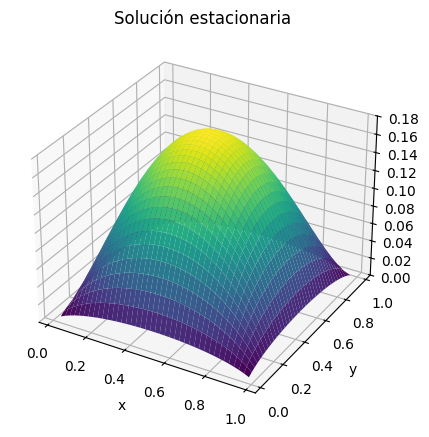
\includegraphics[width=0.5\textwidth]{estacionaria-heat.png}
\caption{Estado estacionario \(u^*\) de la ecuación \(-D\Delta u^* = f\)
con condiciones de borde homogéneas.}
\label{fig:estacionaria-heat}
\end{figure}

La evolución temporal de la solución de la ecuación del calor \(u_t - D\Delta u = f\) se observa en la Figura~\ref{fig:heat2d} para diferentes instantes de tiempo.

\begin{figure}[ht]
\centering
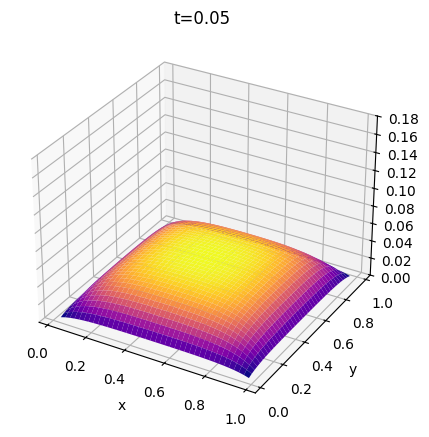
\includegraphics[width=0.4\textwidth]{heat2d-1.png}
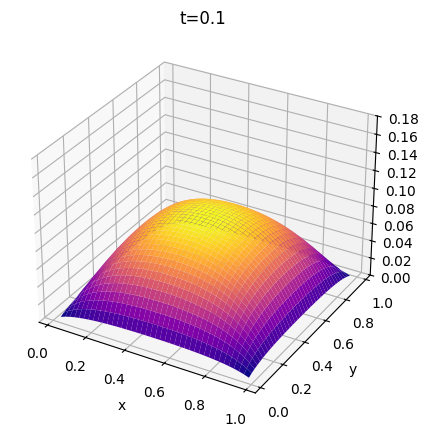
\includegraphics[width=0.4\textwidth]{heat2d-2.png}
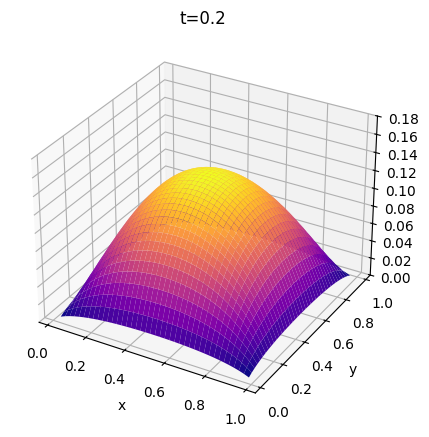
\includegraphics[width=0.4\textwidth]{heat2d-3.png}
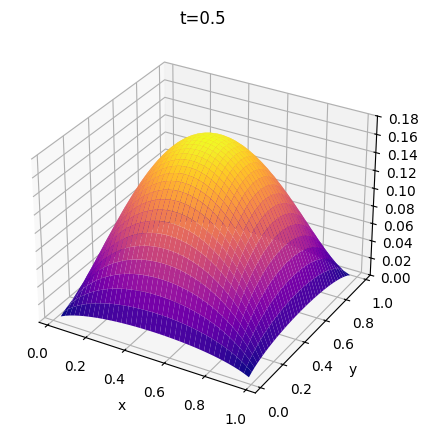
\includegraphics[width=0.4\textwidth]{heat2d-4.png}
\caption{Snapshots de la solución \(u(x,y,t)\) en diferentes tiempos,
mostrando la convergencia hacia el estado estacionario.}
\label{fig:heat2d}
\end{figure}

La Figura~\ref{fig:errores-heat} muestra la evolución de la
norma \(\|u(\cdot,t) - u^*\|_2\) en función del tiempo, ilustrando la
convergencia de la solución temporal hacia el estado estacionario.

\begin{figure}[ht]
\centering
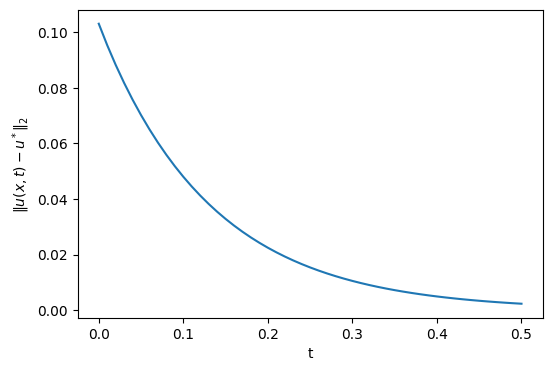
\includegraphics[width=0.5\textwidth]{errores-heat.png}
\caption{Evolución temporal de la norma \(\|u(\cdot,t) - u^*\|_2\),
indicando la convergencia hacia el estado estacionario.}
\label{fig:errores-heat}
\end{figure}

En la Figura~\ref{fig:errores-heat-log} se muestra el gráfico en escala
logarítmica de la norma $\|u(\cdot,t)-u^*\|_2$, que exhibe un decaimiento
exponencial. El ajuste lineal confirma una tasa de decaimiento constante.
\begin{figure}[ht]
\centering
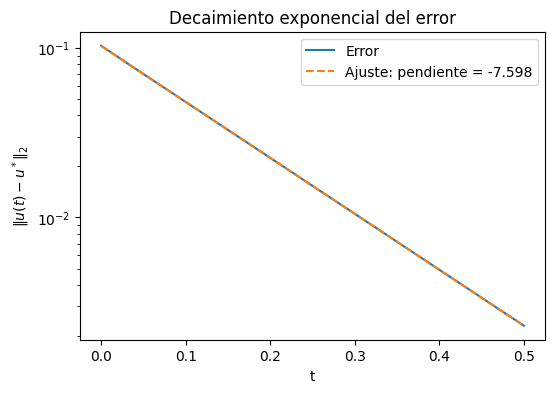
\includegraphics[width=0.5\textwidth]{errores-heat-log.png}
\caption{Gráfico semilogarítmico del error $\|u(\cdot,t)-u^*\|_{L^2(\Omega)}$. La pendiente de la recta ajustada numéricamente representa la tasa de decaimiento exponencial.}
\label{fig:errores-heat-log}
\end{figure}

\subsubsection*{Comparación entre la tasa teórica y la numérica}

Recordemos que, a partir de \eqref{eq:decaimiento-L2}, el régimen transitorio verifica
\[
\|u(\cdot,t)-u^*\|_{L^2(\Omega)}
\;\le\;
\|g-u^*\|_{L^2(\Omega)}\, e^{-\lambda_1 D\, t},
\]
donde $\lambda_1 = \lambda_1(\Omega)$ es la mejor constante de la desigualdad de Poincaré y $D$ es el coeficiente de difusión.

En el dominio considerado, $\Omega = [0,1]\times[0,1]\subset\R^2$, el diámetro es $d=\sqrt{2}$ y en el experimento numérico tomamos $D=0.4$. Usando la cota general $\lambda_1 \ge \pi^2/d^2 = \pi^2/2$ del Teorema~\ref{teo:Poincare}, se obtiene una tasa de decaimiento de al menos
\[
\lambda_1 D \ge 0.2\,\pi^2 \approx 1.97 .
\]
Por otra parte, el ajuste numérico del decaimiento del error (Figura \ref{fig:errores-heat-log}) arroja una tasa bastante mayor, del orden de $7.6$. Esto no contradice la teoría: la cota basada en el diámetro garantiza un decaimiento exponencial, pero no captura la forma del dominio, y por lo tanto no es óptima.

De hecho, para el cuadrado sabemos (Observación \ref{obs:poincare-optima}) que la constante óptima es $\lambda_1 = 2\pi^2$, que da la tasa
\[
\lambda_1 D = 0.8\,\pi^2 \approx 7.90,
\]
en excelente acuerdo con la pendiente $7.6$ observada numéricamente (la pequeña diferencia se debe al error de discretización y a que el ajuste incluye el transitorio inicial, donde contribuyen los modos superiores). En general, la tasa de convergencia al equilibrio de un proceso difusivo en un dominio $\Omega$ está dada por $D\lambda_1(\Omega)$: \emph{el primer autovalor del Laplaciano es la constante de tiempo del dominio}.

\section{Volvemos al problema: la temperatura del suelo}\label{sec:volvemos-suelo}

Consideremos ahora el primer problema conductor de la Sección \ref{sec:conductores-III}. Sea $x\ge 0$ la profundidad y $u(x,t)$ la temperatura del suelo, que suponemos homogéneo con difusividad térmica $D$. Si la temperatura en la superficie es una función conocida $T_s(t)$ (la temperatura del aire, en primera aproximación), el modelo es
\begin{equation}\label{eq:suelo}
\begin{cases}
u_t = D u_{xx}, & x>0,\ t>0,\\
u(0,t) = T_s(t), & t>0,\\
u \text{ acotada cuando } x\to\infty .
\end{cases}
\end{equation}
Por la Parte II sabemos escribir $T_s$ como una suma de oscilaciones: $T_s(t) = \bar T + \sum_k A_k\cos(\omega_k t + \phi_k)$ (con la convención de amplitud y fase de la Sección \ref{sec:ondas-fundamentales}), con $\omega_k$ las frecuencias del ciclo anual, del ciclo diario y de sus armónicos. Como la ecuación es lineal, alcanza con resolver el problema para un forzado de una sola frecuencia, $T_s(t) = \bar T + A\cos(\omega t)$, y superponer.

\subsection*{La solución periódica}

Busquemos una solución de \eqref{eq:suelo} que oscile con la misma frecuencia que el forzado. Con notación compleja, proponemos $u(x,t) = \bar T + \Re\bigl(U(x)e^{i\omega t}\bigr)$. Sustituyendo en la ecuación, $i\omega U = D U''$, cuya solución acotada es $U(x) = A e^{-\sqrt{i\omega/D}\,x}$. Como $\sqrt{i} = (1+i)/\sqrt2$,
$$
U(x) = A\, e^{-x/\delta}\, e^{-i x/\delta},\qquad \delta = \sqrt{\frac{2D}{\omega}},
$$
y tomando parte real obtenemos la \emph{solución periódica}
\begin{equation}\label{eq:suelo-periodica}
u_{per}(x,t) = \bar T + A\, e^{-x/\delta}\cos\Bigl(\omega t - \frac{x}{\delta}\Bigr) .
\end{equation}
La lectura es inmediata y responde las preguntas 2 y 3 de la Sección \ref{sec:conductores-III}:
\begin{itemize}
\item la oscilación se atenúa exponencialmente con la profundidad, con una \emph{profundidad de penetración} $\delta = \sqrt{2D/\omega}$: a profundidad $\delta$ la amplitud es $e^{-1}\simeq 37\%$ de la superficial, y a $3\delta$ es el $5\%$;
\item como $\delta\propto\omega^{-1/2}$, el ciclo anual ($\omega$ unas $365$ veces menor que el diario) penetra $\sqrt{365}\simeq 19$ veces más que el diario. Para un suelo típico, $D\simeq 5\times10^{-7}\,\mathrm{m^2/s}$, lo que da $\delta_{\text{diario}}\simeq 12$ cm y $\delta_{\text{anual}}\simeq 2.2$ m;
\item la oscilación llega con un \emph{retraso de fase} $x/\delta$, es decir un retraso temporal $x/(\delta\omega)$: a profundidad $\delta$ el retraso es $1/\omega$, es decir $1/(2\pi)$ del período (unas $4$ horas para el ciclo diario, unos $2$ meses para el anual). A profundidad $\pi\delta$ la oscilación está en contrafase con la superficie: cuando arriba es verano, ahí abajo es invierno.
\end{itemize}
\figpendiente{Solución periódica de la ecuación del calor en el suelo}{Perfiles $u_{per}(x,t)$ para varios instantes del ciclo (envolvente $e^{-x/\delta}$ marcada) y, en otro panel, la oscilación en función del tiempo a varias profundidades mostrando atenuación y retraso.}

\subsection*{Convergencia al estado periódico}

La función $u_{per}$ es \emph{una} solución de \eqref{eq:suelo}, pero el suelo tiene además una condición inicial $u(x,0)=g(x)$ que en general no coincide con $u_{per}(x,0)$. ¿Qué pasa con la solución verdadera? Acá interviene toda la teoría de este capítulo: la diferencia $v = u - u_{per}$ resuelve la ecuación del calor con condición de borde \emph{homogénea} $v(0,t)=0$ y dato inicial $g - u_{per}(\cdot,0)$. Es exactamente el régimen transitorio que estudiamos, y decae: la solución converge a $u_{per}$ cuando $t\to\infty$, cualquiera sea el dato inicial. En un dominio acotado (una capa de suelo de espesor $H$ sobre una roca a temperatura fija) el decaimiento es exponencial con tasa $D\lambda_1 = D\pi^2/H^2$, por \eqref{eq:decaimiento-L2}; en el semieje el decaimiento es más lento pero igualmente cierto.

Vale la pena detenerse en la moraleja. La ``convergencia al equilibrio'' del título de la sección anterior es, en realidad, convergencia al \emph{atractor} del problema: cuando los datos no dependen del tiempo, el atractor es un estado estacionario; cuando los datos son periódicos, es un estado periódico. En ambos casos el argumento es el mismo (restar el atractor y ver que el resto decae) y la tasa está dada por $D\lambda_1$. Es el mismo esquema que en la Parte I: un equilibrio estable o un ciclo límite estable, ahora en dimensión infinita.

En el laboratorio se ajusta $D$ a partir de registros reales de temperatura a varias profundidades (usando la atenuación y el retraso del ciclo diario) y se compara la predicción \eqref{eq:suelo-periodica} con los datos, lo que responde la pregunta 4. La pregunta 5 (la profundidad a la que enterrar una cañería) se responde con \eqref{eq:suelo-periodica} pidiendo que $\bar T - A e^{-x/\delta} > 0$ para el ciclo anual.

\chapter{La ecuación de Laplace/Poisson}

En este capítulo estudiaremos la ecuación de Laplace/Poisson
\[
-\Delta u = f.
\]
Cuando $f=0$ se la denomina \emph{ecuación de Laplace}, y a sus soluciones se las llama \emph{funciones armónicas}. Cuando $f\neq 0$, se la denomina \emph{ecuación de Poisson}.

Esta ecuación describe los estados estacionarios en la distribución de temperatura (o, más en general, de una sustancia sujeta a un proceso difusivo), pero también aparece en una enorme variedad de contextos físicos, geométricos y probabilísticos, algunos de los cuales iremos explorando a lo largo de este capítulo.

\section{Motivación}\label{sec:minimas}

Existen múltiples motivaciones para el estudio de las ecuaciones de Laplace y de Poisson. En esta sección nos detendremos en dos de ellas.

La primera proviene del estudio de la ecuación de difusión, analizada en el Capítulo \ref{ch:intro-heat}. Como vimos en la sección \ref{sec:heat.n=1} en dimensión uno, y en la sección \ref{sec:convergencia.equilibrio} en dimensiones más altas, en muchos casos la solución de la ecuación del calor converge, cuando $t\to\infty$, a una distribución de equilibrio.

Ese \emph{estado estacionario} es independiente del tiempo y, por lo tanto, debe satisfacer una ecuación elíptica. Más precisamente, verifica la ecuación de Laplace o la ecuación de Poisson, dependiendo de si la fuente $f$ es nula o no. Desde este punto de vista, la ecuación de Laplace/Poisson puede interpretarse como la descripción del equilibrio de un proceso dinámico gobernado por difusión.

Daremos ahora una segunda motivación para el estudio de la ecuación de Laplace, que proviene de un problema clásico de la geometría y del cálculo variacional: el estudio de las \emph{superficies mínimas}.

Supongamos que se tiene un anillo de alambre y se lo sumerge en agua jabonosa. Al retirarlo, se forma una película de jabón adherida al alambre. Una pregunta natural es: ¿cuál es la forma geométrica que adopta dicha película?

Para modelar este problema, asumimos que la película puede describirse como el gráfico de una función de la forma $z=u(x,y)$, con $(x,y)\in D\subset\R^2$, y tal que
\[
u(x,y)=g(x,y)\quad \text{para }(x,y)\in\partial D.
\]
Esta condición refleja el hecho de que la posición de la película en el borde está fijada por el anillo de alambre, cuya forma se supone conocida.

La teoría de superficies mínimas postula que la función $u$ que describe la película es aquella que minimiza el área entre todas las superficies que coinciden con $g$ en el borde.

Recordemos que el área del gráfico de una función $u$ se calcula mediante
\[
\A(u)=\int_D \sqrt{1+|\nabla u|^2}\,dA,
\]
donde $dA=dx dy$ es el diferencial de área.

El problema consiste entonces en encontrar una función $u$ que minimice el funcional $\A$ entre todas las funciones que coinciden con $g$ en $\partial D$ (ver Figura \ref{fig:sup-min}).

\begin{figure}[ht]
\centering
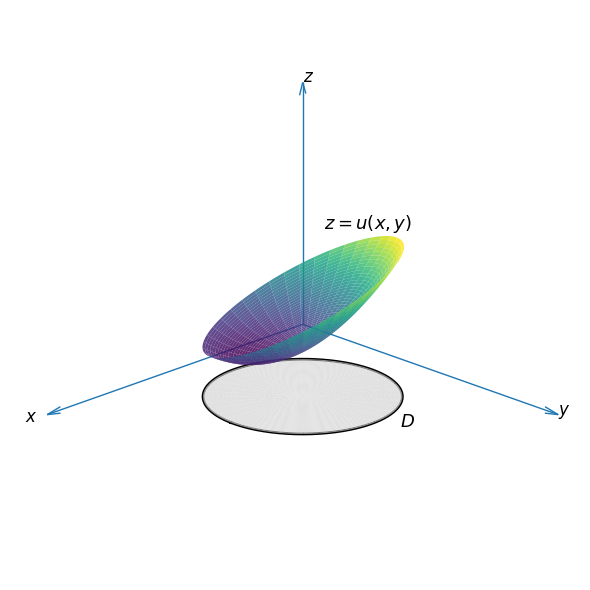
\includegraphics[width=0.4\textwidth]{sup-min1.png}
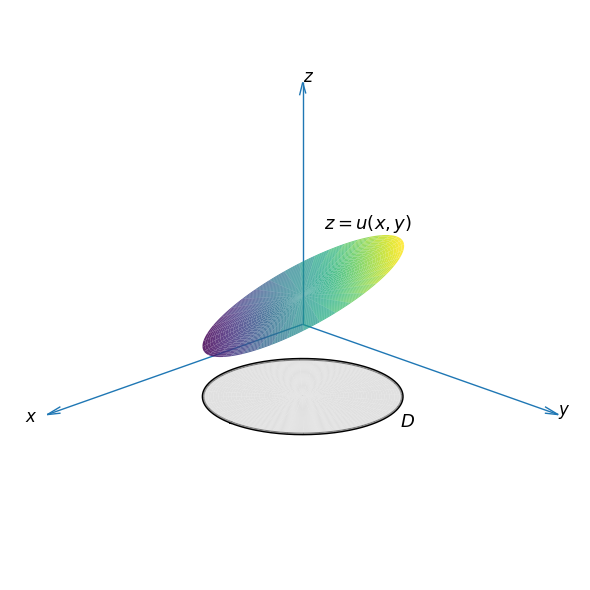
\includegraphics[width=0.4\textwidth]{sup-min2.png}
\caption{Dos superficies con igual condición de contorno. A la izquierda, una superficie arbitraria; a la derecha, una superficie mínima. (Figura a rehacer: en esta versión ambas superficies se ven iguales.)}
\label{fig:sup-min}
\end{figure}

Este problema es, en general, difícil de tratar de manera directa. Entre otras razones, el funcional $\A$ no es uniformemente convexo. Por este motivo, resulta conveniente considerar una aproximación linealizada del problema.

Usando el desarrollo en serie
\[
\sqrt{1+t^2}=1+\frac12 t^2+o(t^2),
\]
y suponiendo que la superficie no presenta oscilaciones grandes (es decir, que $|\nabla u|$ es pequeño), se obtiene la aproximación
\[
\A(u)\simeq \int_D \Big(1+\frac12|\nabla u|^2\Big)\,dA
= \text{área}(D)+\frac12\int_D |\nabla u|^2\,dA.
\]
De este modo, si definimos
\[
\J(u)=\frac12\int_D |\nabla u|^2\,dA,
\]
el problema se reduce a minimizar el funcional $\J$ entre todas las funciones que coinciden con $g$ en $\partial D$. A este funcional se lo denomina la \emph{integral de Dirichlet}.

Supongamos que existe una función $u$ que realiza el mínimo de $\J$ y sea $\phi\in C_c^1(D)$. Para todo $t\in\R$, la función $u+t\phi$ coincide con $g$ en $\partial D$, y por lo tanto
\[
\J(u)\le \J(u+t\phi)\quad \text{para todo }t\in\R.
\]
Definamos $j(t)=\J(u+t\phi)$. Entonces $j\colon\R\to\R$ tiene un mínimo en $t=0$, y en consecuencia $j'(0)=0$. Calculemos esta derivada:
\begin{align*}
j(t)
&=\frac12\int_D |\nabla u+t\nabla\phi|^2\,dA \\
&=\frac12\int_D |\nabla u|^2\,dA
+ t\int_D \nabla u\cdot\nabla\phi\,dA
+ \frac{t^2}{2}\int_D |\nabla\phi|^2\,dA.
\end{align*}
De aquí se deduce que
\[
0=j'(0)=\int_D \nabla u\cdot\nabla\phi\,dA.
\]
Usando el teorema de la divergencia y el hecho de que $\phi$ tiene soporte compacto en $D$, obtenemos
\[
\int_D \nabla u\cdot\nabla\phi\,dA
= -\int_D \Delta u\,\phi\,dA.
\]
Como $\phi\in C_c^1(D)$ es arbitraria, concluimos que
\[
\Delta u = 0 \quad \text{en } D,
\]
es decir, $u$ satisface la ecuación de Laplace.

En situaciones más realistas, la película de jabón no sólo está determinada por la minimización del área, sino que puede estar sometida a fuerzas externas. Un ejemplo típico es la acción de la gravedad, o bien la presencia de una carga distribuida que ejerce una fuerza sobre la superficie.

Supondremos que estas fuerzas son pequeñas y que actúan principalmente en la dirección vertical, es decir, en la dirección del eje $z$. Bajo esta hipótesis, el efecto de la fuerza puede modelarse mediante un término adicional que depende únicamente del valor de la función $u(x,y)$, y no de su gradiente.

Más precisamente, si $f(x,y)$ denota la intensidad de la fuerza (o carga) por unidad de área proyectada sobre el plano $xy$, el trabajo realizado por dicha fuerza puede aproximarse por el funcional
\[
\int_D f(x,y)\,u(x,y)\,dA.
\]
En este contexto, el funcional de energía total del sistema queda dado por
\[
\Ec(u)
= \frac12 \int_D |\nabla u|^2\,dA
- \int_D f(x,y)\,u(x,y)\,dA,
\]
donde el primer término corresponde a la energía asociada a la tensión de la película (integral de Dirichlet) y el segundo término representa el efecto de la fuerza externa.

El problema consiste entonces en encontrar una función $u$ que minimice el funcional $\Ec$ entre todas las funciones que coinciden con $g$ en el borde $\partial D$.

Supongamos que $u$ es un minimizador de $\Ec$ y sea $\phi\in C_c^1(D)$. Para todo $t\in\R$, la función $u+t\phi$ coincide con $g$ en $\partial D$, y por lo tanto
\[
\Ec(u)\le \Ec(u+t\phi).
\]
Definiendo $e(t)=\Ec(u+t\phi)$, la función $e\colon\R\to\R$ tiene un mínimo en $t=0$, lo que implica que $e'(0)=0$. Calculemos esta derivada:
\begin{align*}
e(t)
&= \frac12\int_D |\nabla u+t\nabla\phi|^2\,dA
- \int_D f(x,y)\,(u+t\phi)\,dA \\
&= \frac12\int_D |\nabla u|^2\,dA
+ t\int_D \nabla u\cdot\nabla\phi\,dA
+ \frac{t^2}{2}\int_D |\nabla\phi|^2\,dA \\
&\qquad
- \int_D f(x,y)\,u\,dA
- t\int_D f(x,y)\,\phi\,dA.
\end{align*}
Derivando respecto de $t$ y evaluando en $t=0$, se obtiene
\[
0=e'(0)
= \int_D \nabla u\cdot\nabla\phi\,dA
- \int_D f(x,y)\,\phi\,dA.
\]
Usando nuevamente el teorema de la divergencia y el hecho de que $\phi$ tiene soporte compacto en $D$, resulta
\[
\int_D \nabla u\cdot\nabla\phi\,dA
= -\int_D \Delta u\,\phi\,dA.
\]
Por lo tanto,
\[
\int_D (-\Delta u - f)\,\phi\,dA = 0
\quad\text{para toda }\phi\in C_c^1(D).
\]
Como $\phi$ es arbitraria, concluimos que $u$ satisface la ecuación de Poisson
\begin{equation}\label{eq:poisson}
-\Delta u = f \quad \text{en } D.
\end{equation}

Recíprocamente, supongamos que tenemos una solución de la ecuación de Poisson con condiciones de Dirichlet $u=g$ en $\partial D$. Veamos en entonces $u$ es un mínimo de $\Ec$. En efecto, sea $v$ una función arbitraria tal que $v=g$ en $\partial D$ y definamos $w = v-u$. Entonces $w|_{\partial D}=0$ y tenemos
\[
\begin{aligned}
\Ec(v) - \Ec(u) 
&= \frac12 \int_D |\nabla v|^2 - |\nabla u|^2 \, dA - \int_D f (v-u) \, dA \\
&= \int_D \nabla u \cdot \nabla w \, dA + \frac12 \int_D |\nabla w|^2 \, dA - \int_D f w \, dA.
\end{aligned}
\]

Integrando por partes (Teorema \ref{partes}) y usando que $w|_{\partial D}=0$, se obtiene
\[
\int_D \nabla u \cdot \nabla w \, dA = - \int_D (\Delta u) w \, dA = \int_D f w \, dA.
\]

Por lo tanto,
\[
\Ec(v) - \Ec(u) = \frac12 \int_D |\nabla w|^2 \, dA \ge 0,
\]
lo que muestra que $u$ es efectivamente un mínimo de $\Ec$ entre las funciones que coinciden con $g$ en $\partial D$.

\section{La ecuación de Laplace, juegos aleatorios y valor esperado}\label{sec:juego}

Existe una conexión profunda entre la ecuación de Laplace, los procesos aleatorios y la teoría de juegos, que resulta especialmente natural desde el punto de vista del modelado y del valor esperado.

Consideremos el siguiente juego. Tomamos el cuadrado unitario
\[
Q = [0,1]\times[0,1]\subset\R^2
\]
y lo discretizamos mediante una partición regular. Dado $n\in\N$, definimos
\[
x_i=\frac{i}{n}, \qquad y_j=\frac{j}{n}, \qquad i,j=0,\dots,n,
\]
y consideramos la grilla asociada.

Sea $g\in C(\partial Q)$ una función de pago definida sobre la frontera del cuadrado. Fijado un punto inicial $(x,y)$ de la grilla, el juego evoluciona de la siguiente manera: en cada paso, el jugador se mueve al azar a uno de los cuatro puntos vecinos (arriba, abajo, izquierda o derecha), cada uno con probabilidad $\frac14$. El juego continúa hasta que se alcanza un punto de la frontera $\partial Q$. En ese momento, el jugador cobra el valor $g$ en dicho punto (si $g$ es negativo, el jugador debe pagar).

La pregunta fundamental es: ¿cuál es el precio justo que debería pagarse para poder comenzar el juego en un punto interior $(x,y)$?

Para responderla, introducimos la función $u(x,y)$, definida como el valor esperado del pago final cuando el juego comienza en el punto $(x,y)$. En particular, si $(x,y)\in\partial Q$, el juego termina inmediatamente y
\[
u(x,y)=g(x,y).
\]

Si $(x,y)$ es un punto interior de la grilla, el primer movimiento es aleatorio y conduce, con igual probabilidad, a uno de los cuatro puntos vecinos. Por lo tanto, el valor esperado de comenzar en $(x,y)$ debe coincidir con el promedio de los valores esperados en dichos puntos. Si denotamos $h=\frac{1}{n}$, esta condición se escribe como
\[
u(x,y)
=\frac{u(x+h,y)+u(x-h,y)+u(x,y+h)+u(x,y-h)}{4}.
\]

Esta es una ecuación de equilibrio discreta: el valor del juego en un punto interior es el promedio de los valores en su vecindad inmediata (ver Figura \ref{fig:juego}).
\begin{figure}[ht]
\centering
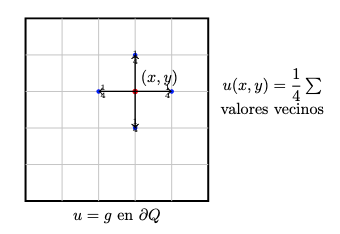
\includegraphics[width=0.4\textwidth]{juego.png}
\caption{Interpretación probabilística de la ecuación de Laplace.
El valor del juego en un punto interior es el promedio de los valores en los puntos vecinos, lo que en el límite continuo conduce a la ecuación $\Delta u = 0$.}
\label{fig:juego}
\end{figure}

Para interpretar esta ecuación en el límite continuo, suponemos que $u$ es una función suficientemente regular y desarrollamos en serie de Taylor alrededor del punto $(x,y)$:
\begin{align*}
u(x\pm h,y) &= u(x,y) \pm \partial_x u(x,y)\,h + \frac12 \partial_{xx}u(x,y)\,h^2 + o(h^2),\\
u(x,y\pm h) &= u(x,y) \pm \partial_y u(x,y)\,h + \frac12 \partial_{yy}u(x,y)\,h^2 + o(h^2).
\end{align*}
Sumando estas expresiones y dividiendo por $4$, obtenemos
\[
u(x,y)
= u(x,y) + \frac{h^2}{4}\,\Delta u(x,y) + o(h^2).
\]
Restando $u(x,y)$ de ambos lados, resulta
\[
0 = \frac{h^2}{4}\,\Delta u(x,y) + o(h^2).
\]
Dividiendo por $h^2$ y tomando el límite cuando $h\to0$, concluimos formalmente que la función $u$ satisface la ecuación de Laplace
\[
\Delta u = 0 \quad \text{en } Q,
\]
junto con la condición de borde de Dirichlet
\[
u = g \quad \text{en } \partial Q.
\]

Desde este punto de vista, las funciones armónicas aparecen naturalmente como funciones de valor esperado de un juego aleatorio: el principio del promedio no es una propiedad misteriosa, sino la traducción matemática del hecho de que no hay ganancia ni pérdida sistemática en el interior del dominio.

Si el juego se modifica introduciendo una ganancia o pérdida sistemática en cada paso —por ejemplo, pagando una pequeña cantidad proporcional a $f(x,y)$ cada vez que el jugador pasa por el punto $(x,y)$—, el balance esperado deja de ser neutro. En ese caso, el valor esperado del juego satisface una ecuación de equilibrio discreta con un término adicional, que en el límite continuo conduce a la ecuación de Poisson
\[
-\Delta u = f.
\]
De este modo, la ecuación de Poisson puede interpretarse como la descripción del valor esperado de un juego aleatorio en presencia de una fuente interna de ganancia o pérdida.

\section{Propiedades analíticas de las soluciones}

En esta sección estudiaremos algunas propiedades fundamentales de las soluciones de la ecuación de Laplace y de la ecuación de Poisson. Estas propiedades garantizan que los problemas que consideramos están bien planteados y, al mismo tiempo, brindan una comprensión cualitativa profunda del comportamiento de las soluciones y de la información que queda determinada por los datos de contorno.

\subsection{Unicidad y métodos integrales}

Comenzamos estudiando resultados de unicidad para soluciones de problemas elípticos bajo distintas condiciones de contorno. La idea central es que, bajo hipótesis naturales, el problema admite a lo sumo una solución, lo que asegura la consistencia del modelo.

Sea $\Omega\subset \R^n$ un dominio regular y consideremos el problema
\[
\begin{cases}
-\Delta u = f & \text{en } \Omega,\\
\mathcal{B}u = g & \text{en } \partial \Omega,
\end{cases}
\]
donde $\mathcal{B}$ denota una condición de contorno que puede ser de alguno de los tipos estudiados en el capítulo previo. En particular:
\begin{itemize}
\item condiciones de tipo Dirichlet,
\[
\mathcal{B}u = u,
\]
\item condiciones de tipo Robin,
\[
\mathcal{B}u = \partial_\n u + \alpha u,\qquad \alpha>0,
\]
\item condiciones mixtas,
\[
\mathcal{B}u =
\begin{cases}
u & \text{en } \partial_D \Omega,\\
\partial_\n u & \text{en } \partial_N \Omega.
\end{cases}
\]
\end{itemize}
Como veremos más adelante, las condiciones de Neumann puras presentan un comportamiento cualitativamente distinto.

La unicidad se prueba típicamente mediante \emph{métodos integrales}. En efecto, si $u_1$ y $u_2$ son dos soluciones del problema, su diferencia $v = u_1 - u_2$ satisface una ecuación homogénea con datos de contorno nulos, es decir,
\[
\begin{cases}
-\Delta v = 0 & \text{en } \Omega,\\
\mathcal{B}v = 0 & \text{en } \partial \Omega.
\end{cases}
\]
Multiplicando la ecuación por $v$ e integrando por partes (Teorema \ref{partes}), se obtiene
\[
0 = -\int_\Omega \Delta v\, v\, d\xx
   = \int_\Omega |\nabla v|^2\, d\xx
     - \int_{\partial\Omega} \partial_\n v\, v\, dS.
\]
Argumentando como en la Sección \ref{sec:unicidad}, se obtiene que
\[
\int_{\partial\Omega} \partial_\n v\, v\, dS = 0
\]
si $\mathcal{B}$ corresponde a condiciones de Dirichlet o mixtas, y que
\[
\int_{\partial\Omega} \partial_\n v\, v\, dS \le 0
\]
si $\mathcal{B}$ es de tipo Robin (acá se usa $\alpha>0$; con $\alpha<0$ la unicidad puede fallar).

En cualquiera de los casos, se concluye que
\[
\int_\Omega |\nabla v|^2\, d\xx \le 0,
\]
lo que implica que $\nabla v = 0$ en $\Omega$, y por lo tanto $v$ es constante (suponemos $\Omega$ conexo). Usando las condiciones de contorno ($v=0$ en una parte de la frontera en los casos Dirichlet y mixto; en el caso Robin, la desigualdad anterior obliga a $\int_{\partial\Omega}\alpha v^2\,dS = 0$, y entonces $v=0$ en el borde), se deduce finalmente que $v=0$, y por ende la solución es única.

Este razonamiento pone de manifiesto el rol central de la integral de Dirichlet como funcional de energía asociado al problema.

\subsection{Condiciones de Neumann y unicidad salvo constantes}

La situación cambia sustancialmente cuando se imponen condiciones de contorno de tipo Neumann,
\[
\partial_\n u = h \quad \text{en } \partial \Omega.
\]
En este caso, si $u$ es solución, entonces $u+C$ también lo es para cualquier constante $C$. En consecuencia, la unicidad sólo puede esperarse \emph{salvo una constante aditiva}.

Efectivamente, si $u_1$ y $u_2$ son dos soluciones del problema de Neumann
\[
-\Delta u = f \quad \text{en } \Omega,
\qquad
\partial_\n u = h \quad \text{en } \partial\Omega,
\]
y definimos $v = u_1 - u_2$, entonces $v$ satisface
\[
-\Delta v = 0 \quad \text{en } \Omega,
\qquad
\partial_\n v = 0 \quad \text{en } \partial\Omega.
\]
Aplicando el mismo argumento integral que en la subsección anterior, se obtiene que $\nabla v = 0$ en $\Omega$, y por lo tanto $v$ es constante. Sin embargo, en este caso no es posible usar la condición de contorno para concluir que dicha constante es nula, ya que cualquier función constante satisface $\partial_\n v = 0$.

Además, en el caso de la ecuación de Poisson con condiciones de Neumann, la existencia de solución requiere que los datos satisfagan una \emph{condición de compatibilidad}. En efecto, integrando la ecuación en el dominio y aplicando el teorema de la divergencia, se obtiene
\[
\int_\Omega f\, d\xx
= -\int_\Omega \Delta u\, d\xx
= -\int_{\partial\Omega} \nabla u \cdot \n\, dS
= -\int_{\partial\Omega} h\, dS.
\]

Esta condición tiene una interpretación física clara. Si $u$ representa la temperatura (o la concentración de una sustancia) en estado estacionario, entonces $f$ describe fuentes o sumideros distribuidos en el interior del dominio, mientras que $\partial_\n u$ representa el flujo de calor (o de materia) a través de la frontera. La condición de compatibilidad expresa que, en un régimen estacionario, la cantidad total producida o absorbida en el interior debe equilibrarse exactamente con el flujo neto a través del borde. Si este balance global no se cumple, no puede existir un estado estacionario.

\subsection{Principio del máximo}

Una de las propiedades más importantes de las funciones armónicas es el \emph{principio del máximo}. Este principio establece, en términos generales, que una función armónica en un dominio acotado alcanza su máximo y su mínimo en la frontera del dominio, y no en el interior (salvo que sea constante). 

\medskip

Comenzamos con una observación elemental.


\begin{obs}
Sea $u\in C^2(\Omega)$ y supongamos que $u$ alcanza un máximo local en un punto $x_0\in\Omega$. Entonces
\[
\partial_{x_i} u(x_0)=0
\qquad\text{y}\qquad
\partial_{x_i x_i} u(x_0)\le 0
\quad\text{para todo } i=1,\dots,n.
\]
En particular,
\[
\Delta u(x_0)=\sum_{i=1}^n \partial_{x_i x_i} u(x_0)\le 0.
\]
\end{obs}

Esta observación conduce inmediatamente al siguiente resultado.

\medskip

\begin{lema}\label{lem:maximo}
Sea $u\in C^2(\Omega)$. Si
\[
\Delta u > 0 \quad \text{en } \Omega,
\]
entonces $u$ no puede alcanzar un máximo en el interior de $\Omega$.
\end{lema}

\begin{proof}
Si $u$ alcanzara un máximo interior en algún punto $x_0\in\Omega$, por la observación anterior debería cumplirse $\Delta u(x_0)\le 0$, lo que contradice la hipótesis $\Delta u>0$ en $\Omega$. Por lo tanto, $u$ no puede tener máximos interiores.
\end{proof}

A partir de este lema se obtiene el principio del máximo para funciones armónicas mediante un argumento de perturbación.

\medskip

\begin{teo}[Principio del máximo]\label{thm:maximo}
Sea $\Omega\subset\R^n$ un abierto acotado y sea $u\in C^2(\Omega)\cap C(\overline{\Omega})$ que verifica
\[
\Delta u \ge 0 \quad \text{en } \Omega.
\]
Entonces
\[
\max_{\overline{\Omega}} u = \max_{\partial\Omega} u.
\]
\end{teo}

\begin{proof}
Sea $\varepsilon>0$ y definamos la función perturbada
\[
u_\varepsilon(x)=u(x)+\varepsilon |x|^2.
\]
Como
\[
\Delta u_\varepsilon = \Delta u + \varepsilon \Delta(|x|^2)\ge 2n\varepsilon >0
\quad \text{en } \Omega,
\]
la función $u_\varepsilon$ satisface las hipótesis del Lema \ref{lem:maximo}. En consecuencia, $u_\varepsilon$ no puede alcanzar un máximo en el interior de $\Omega$, y por lo tanto
\[
\max_{\overline{\Omega}} u_\varepsilon = \max_{\partial\Omega} u_\varepsilon.
\]

Como $u_\ve\rightrightarrows u$ uniformemente cuando $\ve\to 0$ podemos pasar al límite en la igualdad anterior y concluir el resultado deseado.
\end{proof}

Veamos ahora una serie de corolarios que se deducen del Principio del Máximo.

\begin{cor}[Principio del mínimo]\label{cor:minimo}
Sea $u \in C^2(\Omega) \cap C(\overline{\Omega})$ tal que
\[
\Delta u \le 0 \quad \text{en } \Omega.
\]
Entonces
\[
\min_{\overline{\Omega}} u = \min_{\partial \Omega} u.
\]
\end{cor}

\begin{proof}
Aplicamos el principio del máximo a la función $-u$, observando que
\[
\Delta(-u) = -\Delta u \ge 0.
\]
\end{proof}

\medskip

\begin{cor}
Sea $u \in C^2(\Omega) \cap C(\overline{\Omega})$ solución de
\[
-\Delta u = f \quad \text{en } \Omega,\qquad u=g\quad \text{en }\partial\Omega.
\]
Entonces:
\begin{itemize} 
\item Si $f\ge 0$, $u$ satisface el principio del mínimo, es decir,
\[
\min_{\overline{\Omega}} u = \min_{\partial \Omega} g.
\]
\item Si $f\le 0$, $u$ satisface el principio del máximo, es decir,
\[
\max_{\overline{\Omega}} u = \max_{\partial \Omega} g.
\]
\end{itemize}
\end{cor}

\begin{proof}
Inmediata del Teorema \ref{thm:maximo} y el Corolario \ref{cor:minimo}.
\end{proof}

\medskip

\begin{cor}[Principio de comparación]
Sean $u,v \in C^2(\Omega) \cap C(\overline{\Omega})$ tales que
\[
-\Delta u \le -\Delta v \quad \text{en } \Omega,
\qquad
u \le v \quad \text{en } \partial \Omega.
\]
Entonces
\[
u \le v \quad \text{en } \Omega.
\]
\end{cor}

\begin{proof}
Consideramos $w := u - v$. Entonces
\[
-\Delta w \le 0 \quad \text{en } \Omega,
\qquad
w \le 0 \quad \text{en } \partial \Omega.
\]
Por el principio del máximo, se deduce $w \le 0$ en $\Omega$.
\end{proof}

\medskip

\begin{cor}[Unicidad del problema de Dirichlet]
El problema de Dirichlet
\[
\begin{cases}
-\Delta u = f & \text{en } \Omega,\\
u = g & \text{en } \partial \Omega,
\end{cases}
\]
admite a lo sumo una solución en la clase $C^2(\Omega) \cap C(\overline{\Omega})$.
\end{cor}

\begin{proof}
Si $u_1$ y $u_2$ son dos soluciones, entonces $w := u_1 - u_2$ satisface
\[
-\Delta w = 0 \quad \text{en } \Omega,
\qquad
w = 0 \quad \text{en } \partial \Omega.
\]
Por el principio del máximo y del mínimo, se deduce $w \equiv 0$ en $\Omega$.
\end{proof}

\begin{obs}[Interpretación física del principio del máximo]
El principio del máximo tiene una interpretación física muy directa en términos de equilibrio y difusión. 
Si $u$ representa una magnitud que se difunde en el dominio $\Omega$ (por ejemplo, temperatura, potencial eléctrico o altura de una membrana elástica), la condición $\Delta u = 0$ expresa que el sistema se encuentra en equilibrio: no hay fuentes ni sumideros internos.

En este contexto, el valor de $u$ en un punto interior es el resultado de un balance local con su entorno inmediato. En particular, un punto interior no puede ``crear'' espontáneamente un valor mayor (o menor) que los impuestos en el borde, ya que ello requeriría una fuente interna que rompa el equilibrio. 
Por esta razón, los valores extremos de $u$ sólo pueden alcanzarse en la frontera del dominio.

Desde esta perspectiva, el principio del máximo formaliza una idea física elemental: 
en ausencia de fuentes internas, los estados de equilibrio no presentan picos ni valles aislados en el interior del sistema, y los valores extremos están completamente determinados por las condiciones de contorno.
\end{obs}


\subsection{La propiedad del valor medio}

El juego aleatorio de la Sección \ref{sec:juego} decía que el valor de $u$ en un punto es el promedio de sus valores en los cuatro vecinos. La versión continua de esa afirmación es la propiedad más característica de las funciones armónicas.

\begin{teo}[Propiedad del valor medio]\label{teo:valor-medio}
Sea $u\in C^2(\Omega)$ armónica en $\Omega\subset\R^n$. Entonces, para toda bola $B_r(\xx_0)$ con $\overline{B_r(\xx_0)}\subset\Omega$,
$$
u(\xx_0) = \frac{1}{|\partial B_r|}\int_{\partial B_r(\xx_0)} u\, dS = \frac{1}{|B_r|}\int_{B_r(\xx_0)} u\, d\xx :
$$
el valor en el centro es el promedio de los valores sobre cualquier esfera centrada en él, y también el promedio sobre la bola.
\end{teo}

\begin{proof}
Sea $\phi(r)$ el promedio de $u$ sobre la esfera de radio $r$. Con el cambio de variables $\xx = \xx_0 + r\zz$, $|\zz|=1$,
\begin{align*}
&\phi(r) = \frac{1}{|\partial B_1|}\int_{\partial B_1} u(\xx_0+r\zz)\, dS(\zz),\\
&\phi'(r) = \frac{1}{|\partial B_1|}\int_{\partial B_1} \nabla u(\xx_0+r\zz)\cdot\zz\, dS(\zz) = \frac{1}{|\partial B_r|}\int_{\partial B_r(\xx_0)} \partial_\n u\, dS.
\end{align*}
Por el Teorema de la divergencia (Teorema \ref{Gauss}), la última integral es $\int_{B_r(\xx_0)}\Delta u\, d\xx = 0$. Luego $\phi$ es constante, y como $\phi(r)\to u(\xx_0)$ cuando $r\to 0$ (por continuidad de $u$), $\phi(r) = u(\xx_0)$ para todo $r$. La igualdad con el promedio sobre la bola se obtiene integrando en $r$ (coordenadas polares).
\end{proof}

La propiedad del valor medio tiene consecuencias inmediatas. Da una segunda demostración del principio del máximo: si $u$ alcanzara su máximo $M$ en un punto interior $\xx_0$, el promedio de $u$ sobre una bola alrededor de $\xx_0$ sería $M$, lo que obliga a $u\equiv M$ en esa bola, y por conexión en todo $\Omega$ (\emph{principio del máximo fuerte}: una función armónica no constante no alcanza su máximo en el interior). Y explica la regularidad de las funciones armónicas: $u$ es en cada punto un promedio de sí misma, y promediar suaviza; de hecho toda función armónica es $C^\infty$ (y aun analítica). La misma idea en versión discreta es la que hace funcionar los métodos numéricos de la Sección \ref{sec:juego} (ejercicios de laboratorio) y los algoritmos de propagación de etiquetas en grafos.

\section{La solución fundamental y el principio de superposición}

En esta sección presentamos una herramienta conceptual que permite interpretar la ecuación de Poisson como la superposición de los efectos producidos por fuentes elementales. No entraremos en detalles técnicos, sino que nos concentraremos en su significado físico y geométrico.

Comencemos con un concepto fundamental: la ``función'' \emph{delta de Dirac} $\delta_0(\xx)$, introducida por Dirac en el estudio de mecánica cuántica \cite{Dirac}.

\begin{defi}[``función'' delta de Dirac]\label{def:dirac}
Se define informalmente la ``función'' delta de Dirac $\delta_0\colon \R^n\to\R$ como un objeto que verifica:
\begin{itemize}
\item $\delta_0(\xx) = 0$ si $\xx\neq 0$, y $\delta_0(0)$ es ``infinitamente grande''.
\item $\int_{\R^n} \delta_0(\xx)\, d\xx = 1$.
\item Para cualquier función continua y de soporte compacto $f\colon \R^n\to\R$, 
$$
\int_{\R^n} f(\xx)\,\delta_0(\xx)\, d\xx = f(0).
$$
\end{itemize}
\end{defi}

\begin{obs}
Esta definición es informal; basta pensar en $\delta_0$ como un símbolo con las propiedades anteriores. Dirac introdujo este concepto en mecánica cuántica (que le valió el premio Nobel en 1933), pero no fue sino hasta mediados del siglo XX que, con el desarrollo de la teoría de distribuciones por Schwartz \cite{Schwartz}, este concepto pudo ser formalizado matemáticamente; dicho trabajo le valió la Medalla Fields en 1950. Una definición más precisa, en el marco de la teoría de distribuciones, puede encontrarse en \cite{Bonder}.
\end{obs}

\medskip

Consideremos ahora el problema
\[
-\Delta \Phi = \delta_0 \quad \text{en } \R^n,
\]
donde \(\Phi\) se denomina \emph{solución fundamental} del Laplaciano. Intuitivamente, \(\Phi\) representa la respuesta de un sistema frente a una fuente puntual unitaria. Por ejemplo, en conducción de calor, corresponde a la temperatura estacionaria generada por una fuente infinitesimal en un punto; en electrostática, representa el potencial producido por una carga puntual. 

Sin entrar en derivaciones técnicas, las solución fundamental viene dada por
\[
\Phi(\xx) = 
\begin{cases}
-\frac{1}{2\pi} \log |\xx|, & n=2,\\[1em]
\frac{1}{n(n-2)\omega_n} \frac{1}{|\xx|^{n-2}}, & n\ge 3,
\end{cases}
\]
donde $\omega_n$ es el volumen de la esfera de radio 1 en dimensión $n$ (por ejemplo, $\omega_3 = \frac43\pi$). Estas funciones son suaves fuera del origen y presentan una singularidad donde se concentra la fuente. Ver \cite{Bonder} para una deducción de las mismas. 
\begin{figure}[h]
\centering
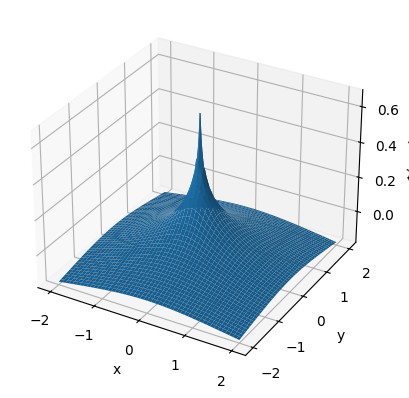
\includegraphics[width=0.4\textwidth]{sol-fundamental-lap.png}
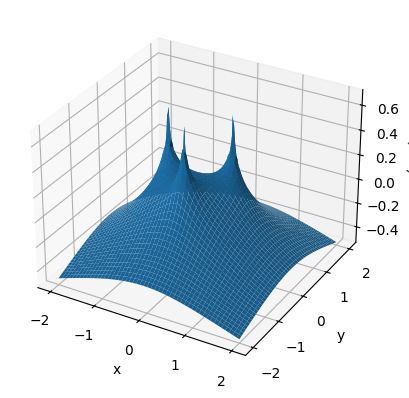
\includegraphics[width=0.4\textwidth]{superposicion.png}
\caption{A la izquierda, solución fundamental del Laplaciano en dimensión $2$ y a la derecha solución de la ecuación de Poisson asociada a tres cargas puntuales, obtenida por superposición de las soluciones fundamentales correspondientes.}
\label{fig:sol-fundamental2}
\end{figure}

Una consecuencia inmediata de esta interpretación es el principio de superposición. Si se consideran varias fuentes puntuales ubicadas en distintas posiciones, la respuesta total del sistema se obtiene sumando las contribuciones individuales. Desde el punto de vista físico, esto refleja que el efecto de varias cargas o fuentes se acumula linealmente. Ver Figura \ref{fig:sol-fundamental2}.

Este razonamiento puede extenderse a una distribución continua de fuentes. En ese caso, una fuente dada por una función \(f\) puede pensarse como la superposición de infinitas fuentes puntuales ponderadas por \(f\). Formalmente, esto se expresa como
\[
u(x) = \int_{\R^n} \Phi(x-y)\, f(y)\, dy,
\]
lo que implica que
\[
-\Delta u = f \quad\text{en } \R^n.
\]
Es decir, la solución se obtiene como la \emph{convolución} de \(f\) con la solución fundamental. Notemos que esta fórmula resuelve la ecuación en \emph{todo el espacio}: en un dominio acotado $\Omega$ la función $\Phi*f$ satisface $-\Delta u = f$ en $\Omega$ pero no cumple ninguna condición de borde prescripta, y hay que corregirla sumándole una función armónica adecuada (el mismo procedimiento que en la Sección \ref{sec:convergencia.equilibrio}, con el papel del estado estacionario invertido).

Desde esta perspectiva, el operador \emph{inverso} de $-\Delta$, es decir la convolución con $\Phi$, actúa como un operador suavizante: aun cuando la fuente presente irregularidades o ruido, la solución resultante es más regular y suave, ya que cada valor de \(u\) se obtiene como una media ponderada de la fuente en todo el dominio. Ver Figura \ref{fig:convolucion}. (El operador $-\Delta$ mismo hace lo contrario: deriva dos veces y amplifica las irregularidades; es su inversa la que suaviza, exactamente como en la Sección \ref{sec:convergencia.equilibrio} vimos que la ecuación del calor suaviza mientras que ``correrla hacia atrás'' amplifica.)

\begin{figure}[h]
\centering
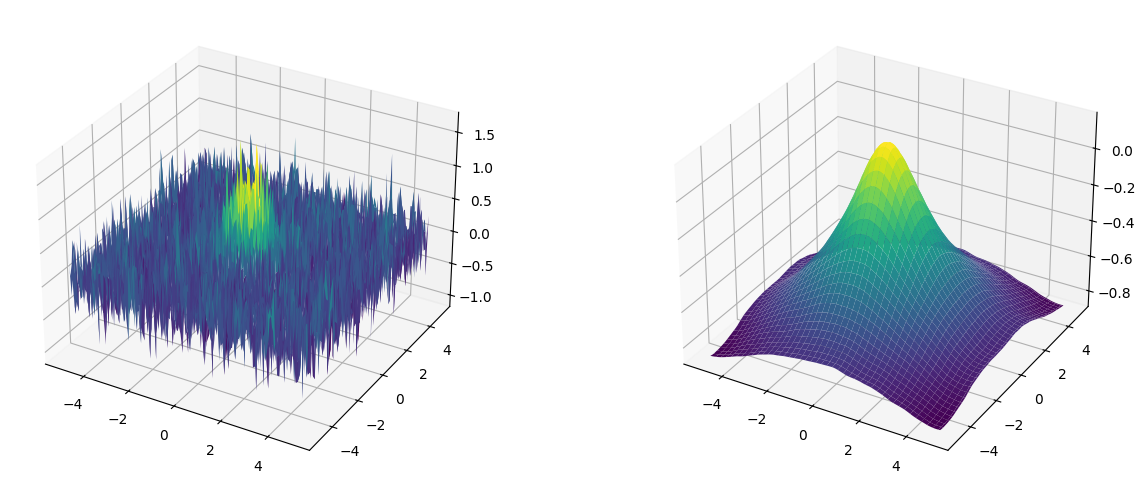
\includegraphics[width=0.8\textwidth]{convolucion.png}
\caption{Fuente $f$ ruidosa (izquierda) y solución de la ecuación de Poisson asociada (derecha) $u=\Phi*f$, ilustrando el efecto suavizante del operador Laplaciano.}
\label{fig:convolucion}
\end{figure}



\section{Resolución mediante series de Fourier en un rectángulo}

En esta sección mostramos cómo resolver explícitamente la ecuación de Poisson en un dominio rectangular utilizando series de Fourier. El procedimiento es una extensión directa del método visto anteriormente en una dimensión y se basa en una idea simple pero fundamental: si se dispone de una base ortogonal de $L^2$ en un intervalo, entonces se puede construir de manera natural una base ortogonal de $L^2$ en un rectángulo tomando productos de funciones.

\medskip

Recordemos primero el caso unidimensional. En el intervalo $(0,L)$, las funciones
\[
\phi_k(x) = \sin\!\Big(\frac{k\pi x}{L}\Big),
\qquad k\in\N,
\]
forman una base ortogonal de $L^2(0,L)$ y son autofunciones del operador $-\frac{d^2}{dx^2}$ con condiciones de contorno de Dirichlet homogéneas. En el capítulo anterior vimos cómo esta propiedad permite resolver la ecuación del calor en una dimensión descomponiendo las funciones involucradas en esta base.

La situación en dos dimensiones es conceptualmente análoga. Consideremos ahora el rectángulo
\[
\Omega = (0,L)\times(0,H)\subset\R^2.
\]
Si tomamos una base ortogonal de $L^2(0,L)$ y una base ortogonal de $L^2(0,H)$, entonces los productos de funciones de ambas bases generan una base ortogonal de $L^2(\Omega)$. En particular, las funciones
\[
\phi_{k,\ell}(x,y)
=
\sin\!\Big(\frac{k\pi x}{L}\Big)\,
\sin\!\Big(\frac{\ell\pi y}{H}\Big),
\qquad k,\ell\in\N,
\]
forman una base ortogonal de $L^2(\Omega)$ y se anulan sobre el borde del rectángulo, por lo que están naturalmente adaptadas a condiciones de contorno de Dirichlet homogéneas.

Además, esta base diagonaliza al operador Laplaciano. En efecto, cada función $\phi_{k,\ell}$ es una autofunción de $-\Delta$ y se tiene
\[
-\Delta \phi_{k,\ell}
=
\lambda_{k,\ell}\,\phi_{k,\ell},
\qquad
\lambda_{k,\ell}
=
\Big(\frac{k\pi}{L}\Big)^2
+
\Big(\frac{\ell\pi}{H}\Big)^2.
\]
Este hecho es crucial, ya que permite transformar una ecuación diferencial en una colección de ecuaciones algebraicas independientes.

\medskip

Consideremos entonces el problema de Poisson con condiciones de contorno de Dirichlet homogéneas
\[
\begin{cases}
-\Delta u = f & \text{en } \Omega,\\
u = 0 & \text{en } \partial \Omega.
\end{cases}
\]
Supondremos que la fuente $f$ pertenece a $L^2(\Omega)$ y la descomponemos en la base anterior:
\[
f(x,y)
=
\sum_{k,\ell\ge 1}
f_{k,\ell}\,\phi_{k,\ell}(x,y),
\]
donde los coeficientes de Fourier están dados por
\[
f_{k,\ell}
=
\frac{4}{LH}
\int_0^L\int_0^H
f(x,y)\,
\phi_{k,\ell}(x,y)\,dx\,dy.
\]

Buscamos una solución $u$ con un desarrollo análogo,
\[
u(x,y)
=
\sum_{k,\ell\ge 1}
u_{k,\ell}\,\phi_{k,\ell}(x,y).
\]
Al sustituir estas expresiones en la ecuación $-\Delta u = f$ y utilizar que el Laplaciano actúa de forma diagonal sobre la base $\{\phi_{k,\ell}\}$, obtenemos para cada par $(k,\ell)$ la ecuación algebraica
\[
\lambda_{k,\ell}\,u_{k,\ell} = f_{k,\ell}.
\]
De aquí se sigue inmediatamente que
\[
u_{k,\ell} = \frac{f_{k,\ell}}{\lambda_{k,\ell}},
\]
lo que determina completamente la solución.

\medskip

Este procedimiento permite interpretar la ecuación de Poisson de manera muy clara: resolver $-\Delta u = f$ equivale a descomponer la fuente en modos de Fourier y dividir cada modo por su autovalor correspondiente. Como los autovalores crecen con la frecuencia, los modos de alta frecuencia quedan fuertemente amortiguados, lo que explica una vez más el carácter suavizante del operador elíptico.

En la Figura~\ref{fig:poisson-fourier} se muestra una aproximación de la solución de la ecuación de Poisson con condiciones de Dirichlet homogéneas y fuente $f(x,y)=-x\,e^{x+y}$, obtenida truncando la serie de Fourier a los primeros 20 modos. Observamos que, dado que la fuente es negativa, el principio del máximo implica que la solución también es negativa, en completo acuerdo con la simulación numérica.

\begin{figure}[ht]
\centering
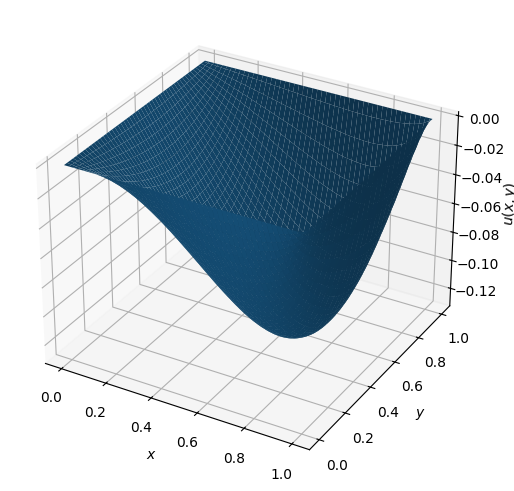
\includegraphics[width=0.4\textwidth]{poisson-fourier.png}
\caption{Aproximación de la solución de la ecuación de Poisson $\Delta u = f$ con condiciones de Dirichlet homogéneas mediante 20 nodos de la expansión en serie de Fourier. La fuente es $f(x,y)=-x\, e^{x+y}$.}
\label{fig:poisson-fourier}
\end{figure}



\chapter{Ecuaciones hiperbólicas: la ecuación de ondas}

Las \emph{ecuaciones hiperbólicas} modelan fenómenos donde la información o perturbaciones se propagan con velocidad finita a través de un medio. El ejemplo más clásico es la \emph{ecuación de ondas}, que describe cómo se propagan vibraciones en cuerdas, membranas, sólidos elásticos o incluso ondas sonoras y electromagnéticas. 

La ecuación de ondas fue uno de los primeros ejemplos de ecuaciones diferenciales parciales estudiadas de manera sistemática. En 1747, Jean le Rond d'Alembert \cite{dAlembert} introdujo el método de las características para resolver la ecuación de la cuerda vibrante en toda la recta, obteniendo una fórmula explícita que expresa la solución como la superposición de dos ondas viajeras. Este resultado, conocido hoy como la \emph{fórmula de d'Alembert}, constituye uno de los hitos fundacionales en la teoría de las ecuaciones en derivadas parciales.

En este capítulo primero discutiremos distintos tipos de ondas y sus propiedades, antes de deducir formalmente la ecuación de ondas y explorar métodos de resolución en una dimensión. 


\section{Tipos de ondas}

En la vida cotidiana nos encontramos con distintos tipos de ondas: ondas sonoras, ondas electromagnéticas (como ondas de radio o de luz), ondas en el agua (profundas o superficiales) y ondas elásticas en sólidos. Fenómenos oscilatorios aparecen también en contextos menos evidentes, como ondas de rarefacción o de choque en dinámica de tráfico, ondas electroquímicas en el sistema nervioso o en la regulación del latido cardíaco, e incluso, a escala cuántica, todo puede describirse mediante funciones de onda. Ver la figura pendiente al final de este párrafo.

\figpendiente{Distintos tipos de ondas}{Tres fotos o esquemas propios (cuerda, agua, onda electromagnética) en reemplazo de las imágenes de origen externo de la versión anterior.}


Aunque estos fenómenos comparten ciertas características, también presentan diferencias importantes. Por ejemplo, las ondas progresivas en el agua propagan una perturbación, mientras que las ondas estacionarias no. Las ondas sonoras requieren un medio material, mientras que las ondas electromagnéticas no. Las ondas electroquímicas suelen interactuar con el medio, modificándolo, mientras que las ondas en el agua no.

Por estas razones, es difícil dar una definición única de \emph{onda} que abarque todos los casos anteriores. Nos limitaremos a introducir terminología y conceptos generales, relacionados con tipos específicos de ondas, empezando por ondas unidimensionales.

\subsection*{Ondas viajeras o progresivas}
Son perturbaciones que se describen mediante una función de la forma
\[
u(x,t) = g(x - ct),
\]
donde $c$ es la velocidad de propagación. Para $t=0$, la función $u(x,0)=g(x)$ representa el perfil inicial de la perturbación, que se propaga sin deformarse con velocidad $|c|$ en la dirección positiva ($c>0$) o negativa ($c<0$) de $x$. Ver Figura \ref{fig:viajera}.
\begin{figure}[ht]
\centering
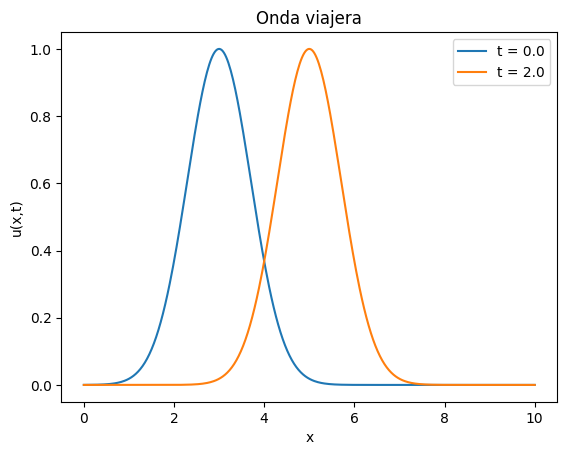
\includegraphics[width=0.5\textwidth]{viajera.png}
\caption{Una onda viajera en una dimensión. El perfil inicial se desplaza rigidamente en el espacio con velocidad constante, sin cambiar de forma.}
\label{fig:viajera}
\end{figure}

\subsection*{Ondas armónicas}
Son un caso particular de ondas progresivas:
\[
u(x,t) = A \cos(kx - \omega t),
\]
donde $A$ es la amplitud, $k$ el número de onda, $\omega$ la frecuencia angular y $\lambda = 2\pi/k$ la longitud de onda. La velocidad de fase es $c_p = \omega/k$. La notación compleja $u(x,t) = A e^{i(kx - \omega t)}$ puede simplificar los cálculos. Ver Figura \ref{fig:armonica}.
\begin{figure}[ht]
\centering
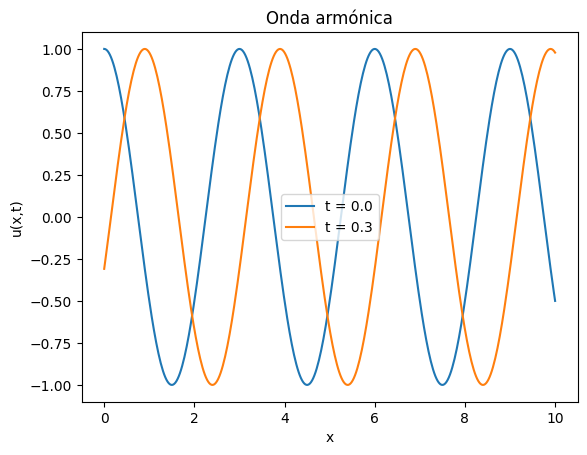
\includegraphics[width=0.5\textwidth]{armonica.png}
\caption{Dos instantáneas de una onda armónica en distintos instantes de tiempo. Se trata de un caso particular de onda viajera, caracterizado por una dependencia sinusoidal en el espacio.}
\label{fig:armonica}
\end{figure}

\subsection*{Ondas estacionarias}
Se pueden generar, por ejemplo, superponiendo dos ondas armónicas de igual amplitud que se propagan en direcciones opuestas:
\[
u(x,t) = A \cos(kx - \omega t) + A \cos(kx + \omega t) = 2 A \cos(kx) \cos(\omega t).
\]
Aquí, la onda básica $\cos(kx)$ se modula en el tiempo mediante $B \cos(\omega t)$. Ver Figura \ref{fig:estacionaria}.
\begin{figure}[ht]
\centering
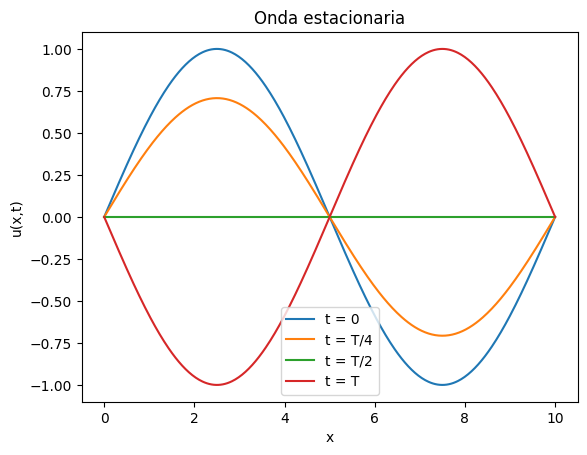
\includegraphics[width=0.5\textwidth]{estacionaria.png}
\caption{Instantáneas de una onda estacionaria en distintos instantes. La forma espacial permanece fija y la oscilación ocurre únicamente en el tiempo, sin transporte neto de la perturbación.}
\label{fig:estacionaria}
\end{figure}

\subsection*{Ondas en más de una dimensión}
\paragraph{\bf Ondas planas}
En dimensión $n>1$, una onda plana se puede escribir como
\[
u(\mathbf{x},t) = f(\mathbf{k}\cdot \mathbf{x} - \omega t),
\]
donde $\mathbf{k}$ es el vector de onda y $\mathbf{k}/|\mathbf{k}|$ indica la dirección de propagación. La velocidad de fase es $c_p = \omega/|\mathbf{k}|$. En el caso armónico:
\[
u(\mathbf{x},t) = A e^{i(\mathbf{k}\cdot \mathbf{x} - \omega t)}.
\]
Ver Figura \ref{fig:plana}.
\begin{figure}[ht]
\centering
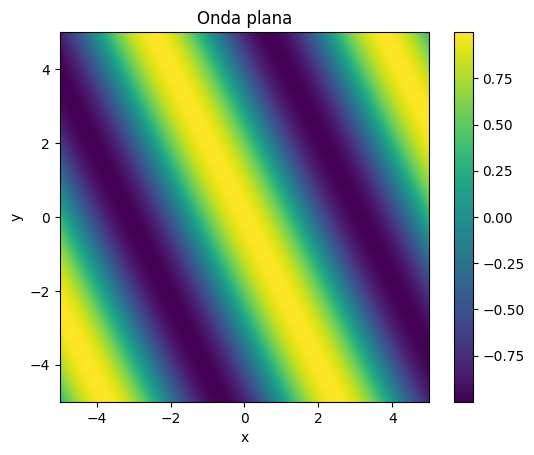
\includegraphics[width=0.5\textwidth]{plana.png}
\caption{Instantánea de una onda plana en dos dimensiones. Los frentes de onda son líneas paralelas, lo que indica una propagación en una dirección fija.}
\label{fig:plana}
\end{figure}

\paragraph{\bf Ondas esféricas}
Dependen únicamente de la distancia $r = |\mathbf{x} - \mathbf{x}_0|$ a un punto fijo $\mathbf{x}_0 \in \mathbb{R}^n$:
\[
u(\mathbf{x},t) = v(r,t).
\]
Por ejemplo, una onda esférica estacionaria puede escribirse $u(\mathbf{x},t) = e^{i\omega t} v(r)$, mientras que una onda esférica progresiva toma la forma $u(\mathbf{x},t) = v(r - ct)$, cuyas superficies de onda son esferas $r - ct = \text{constante}$. Ver Figura \ref{fig:esferica}.
\begin{figure}[ht]
\centering
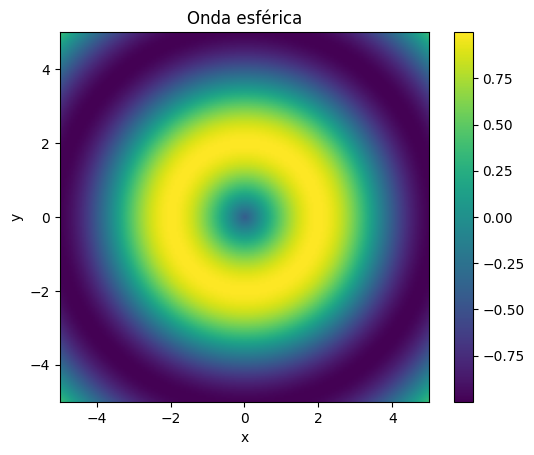
\includegraphics[width=0.5\textwidth]{esferica.png}
\caption{Instantánea de una onda esférica en dos dimensiones. La perturbación se propaga radialmente desde una fuente puntual, dando lugar a frentes de onda concéntricos.}
\label{fig:esferica}
\end{figure}

\section{Motivación}

La ecuación de ondas describe cómo se propaga una perturbación en un medio elástico. En una dimensión espacial, puede deducirse desde dos perspectivas complementarias: un modelo discreto de partículas conectadas por resortes, o un modelo continuo basado en el balance de fuerzas en una cuerda.



\subsection{Deducción a partir de partículas y resortes}

La ley de Hook modela el desplazamiento de una partícula sujeta a un resorte. Sea $x(t)$ el desplazamiento de una partícula de masa $m$ respecto de su posición de equilibrio. La fuerza que aplica el resorte es proporcional al desplazamiento y apunta en sentido opuesto:
\[
F = -\kappa x,
\]
donde $\kappa>0$ es la constante del resorte. La segunda ley de Newton ($F = ma$) da:
\[
m x''(t) + \kappa x(t) = 0.
\]

Ahora consideremos una cuerda como un arreglo de pequeñas masas $m$ conectadas por resortes sin masa de longitud $h$ y constante $\kappa$ (ver Figura \ref{fig:ondas-resorte}). Sea $u(x,t)$ el desplazamiento de la masa situada en $x$ a tiempo $t$. La fuerza resultante sobre esta partícula es
\[
F = \kappa [u(x+h,t)-u(x,t)] - \kappa [u(x,t)-u(x-h,t)] = \kappa [u(x+h,t)-2u(x,t)+u(x-h,t)].
\]

\begin{figure}[ht]
\centering
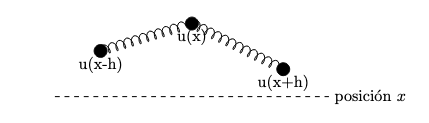
\includegraphics[width=0.5\textwidth]{ondas-resorte.png}
\caption{Esquema de una cuerda modelada como partículas unidas por resortes, con posiciones desplazadas para representar vibraciones.}
\label{fig:ondas-resorte}
\end{figure}


Por la ley de Newton,
\[
m u_{tt}(x,t) = \kappa [u(x+h,t)-2u(x,t)+u(x-h,t)].
\]

Si la cuerda tiene longitud $L=Nh$ y masa total $M=Nm$, y definimos la constante efectiva $k = \kappa/N$, la ecuación se puede escribir como
\[
u_{tt}(x,t) = \frac{L^2 k}{M} \frac{u(x+h,t)-2u(x,t)+u(x-h,t)}{h^2}.
\]

Finalmente, tomando el límite $h \to 0$ obtenemos la ecuación de ondas continua:
\begin{equation}\label{eq:ondas}
u_{tt}(x,t) = c^2 u_{xx}(x,t), 
\end{equation}
donde $c = \sqrt{\frac{L^2 k}{M}}$.

\subsection{Deducción de la ecuación de ondas mediante balance de tensiones}

Veamos otra deducción de la ecuación de ondas. Consideremos una cuerda de longitud $\ell$ y densidad lineal de masa $\rho=\rho(x)$ (constante si la cuerda es homogénea). Asumamos que la cuerda se mueve en la dirección transversal, pero no en la dirección longitudinal. Notemos por $u(x,t)$ el desplazamiento en la posición $x$ a tiempo $t$ en la dirección transversal de su equilibrio. La pendiente de la cuerda a tiempo $t$ en la posición $x$ se denota por $\partial_x u(x,t)$. Sea $T(x,t)$ la magnitud de la tensión (fuerza) tangencial aplicada sobre la cuerda a tiempo $t$ en la posición $x$ (ver Figura \ref{fig:ondas-tension}).
\begin{figure}[ht]
\centering
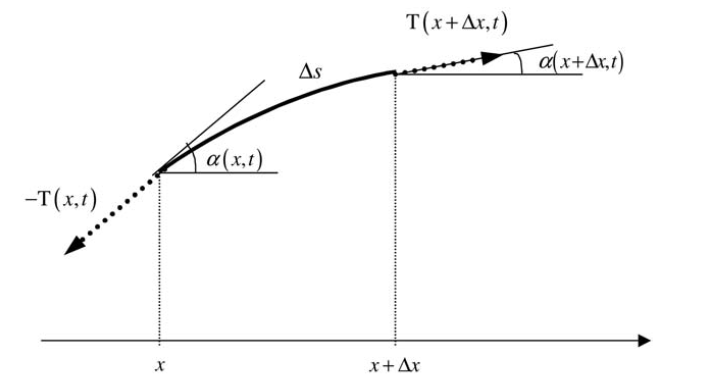
\includegraphics[width=0.6\textwidth]{ondas-tension.png}
\caption{Tensión en los puntos extremos de un segmento pequeño de una cuerda.}
\label{fig:ondas-tension}
\end{figure}

Consideremos la porción de la cuerda entre dos puntos próximos $x_1$ y $x_2$. La fuerza neta que actúa sobre la cuerda en la dirección longitudinal, notada por $F_1$, está dada por
\begin{align*}
F_1|_{x_1}^{x_2} &= T(x,t)\cos\theta \Big|_{x_1}^{x_2} = T(x,t) \frac{1}{\sqrt{1 + (\partial_x u)^2}}\Big|_{x_1}^{x_2} \\
&= T(x_2,t) \frac{1}{\sqrt{1 + (\partial_x u(x_2,t))^2}} - T(x_1,t) \frac{1}{\sqrt{1 + (\partial_x u(x_1,t))^2}}.
\end{align*}
Por hipótesis, la cuerda no se desplaza en la dirección longitudinal, por lo que la aceleración en esa dirección es cero. Entonces, usando la ley de Newton, $\mathbf F = m\mathbf a$, se obtiene
\begin{equation}\label{F.longitudinal}
F_1|_{x_1}^{x_2} = T(x_2,t) \frac{1}{\sqrt{1 + (\partial_x u(x_2,t))^2}} - T(x_1,t) \frac{1}{\sqrt{1 + (\partial_x u(x_1,t))^2}} = 0.
\end{equation}

En la dirección transversal, la fuerza que actúa sobre la cuerda entre los puntos $x_1$ y $x_2$, denotada por $F_2$, es
\begin{align*}
F_2|_{x_1}^{x_2} &= T(x,t)\sin\theta \Big|_{x_1}^{x_2} = T(x,t) \frac{\partial_x u}{\sqrt{1 + (\partial_x u)^2}}\Big|_{x_1}^{x_2} \\
&= T(x_2,t) \frac{\partial_x u(x_2,t)}{\sqrt{1 + (\partial_x u(x_2,t))^2}} - T(x_1,t) \frac{\partial_x u(x_1,t)}{\sqrt{1 + (\partial_x u(x_1,t))^2}}.
\end{align*}
Asumiendo que todo el desplazamiento ocurre en la dirección transversal, la ley de Newton nos da $F_2(x,t) = m a_2(x,t)$, donde $a_2(x,t)$ es la componente de la aceleración de la cuerda en la dirección transversal. Entre los puntos $x_1$ y $x_2$,
\[
F_2|_{x_1}^{x_2} = \int_{x_1}^{x_2} \rho(x) \partial_{tt} u(x,t)\, dx.
\]
Así, obtenemos
\begin{equation}\label{F.transversal}
T(x_2,t) \frac{\partial_x u(x_2,t)}{\sqrt{1 + (\partial_x u(x_2,t))^2}} - T(x_1,t) \frac{\partial_x u(x_1,t)}{\sqrt{1 + (\partial_x u(x_1,t))^2}} = \int_{x_1}^{x_2} \rho(x) \partial_{tt} u(x,t)\, dx.
\end{equation}

Si asumimos que $\partial_x u$ es pequeño (pequeñas vibraciones de la cuerda), se tiene
\[
\sqrt{1 + (\partial_x u)^2} \simeq 1,
\]
y de \eqref{F.transversal} se sigue
\[
T(x_2,t) \partial_x u(x_2,t) - T(x_1,t) \partial_x u(x_1,t) \simeq \int_{x_1}^{x_2} \rho(x) \partial_{tt} u(x,t)\, dx.
\]
Dividiendo entre $x_2 - x_1$ y tomando el límite $x_2 \to x_1$,
\begin{equation}\label{pre.ondas}
\partial_x(T \partial_x u) = \rho \partial_{tt} u.
\end{equation}

Por \eqref{F.longitudinal}, para valores pequeños de $\partial_x u$, se puede suponer que $T$ es independiente de $x$. Si además $T$ es constante en el tiempo y $\rho$ es constante, \eqref{pre.ondas} se simplifica a
\[
\partial_{tt} u = \frac{T}{\rho} \partial_{xx} u.
\]
Definiendo $c = \sqrt{\frac{T}{\rho}}$, se llega nuevamente a la ecuación \eqref{eq:ondas}.

\subsection*{Condiciones iniciales y de contorno}

Al igual que con la ecuación del calor y con las ecuaciones de Laplace y Poisson, cuando el dominio en el cual ocurre el fenómeno es acotado resulta necesario describir la interacción del sistema con el entorno. Esto se realiza mediante la imposición de condiciones de contorno.

Asumiremos en lo que sigue que estamos en el caso unidimensional y que la ecuación de ondas \eqref{eq:ondas} está planteada en el intervalo $(0,L)$. Existen distintos tipos de condiciones de contorno, según el tipo de interacción física que se modele.

\begin{itemize}
\item \textbf{Condiciones de Dirichlet.}  
En este caso se prescribe la posición de la cuerda en los extremos del intervalo:
\[
u(0,t)=a(t), \qquad u(L,t)=b(t).
\]
Físicamente, esto corresponde a suponer que los extremos de la cuerda están fijados y forzados a seguir trayectorias dadas por $a(t)$ y $b(t)$.  
Cuando $a=b=0$ se dice que la condición es \emph{homogénea}, y representa una cuerda fija en reposo en ambos extremos.

\item \textbf{Condiciones de Neumann.}  
En este caso se prescribe la derivada espacial de la solución en los extremos:
\[
- u_x(0,t) = \alpha(t), \qquad u_x(L,t) = \beta(t).
\]
Desde el punto de vista físico, estas condiciones representan la prescripción de la fuerza (o tensión) ejercida sobre los extremos de la cuerda. En particular, cuando $\alpha(t)=\beta(t)=0$, los extremos son libres, ya que no actúa ninguna fuerza externa sobre ellos.

\item \textbf{Condiciones de Robin.}  
Estas condiciones combinan las anteriores y tienen la forma
\[
- u_x(0,t) + \kappa u(0,t) = a(t), \qquad 
u_x(L,t) + \kappa u(L,t) = b(t),
\]
donde $\kappa>0$ es un parámetro.  
Desde el punto de vista físico, este tipo de condición modela un extremo de la cuerda conectado a un resorte: la fuerza ejercida sobre el extremo es proporcional a su desplazamiento. El término con $u_x$ representa la tensión de la cuerda, mientras que el término proporcional a $u$ representa la fuerza restauradora del resorte.
\end{itemize}

Por supuesto, estas condiciones pueden combinarse, imponiendo distintos tipos de condiciones en cada extremo del intervalo.


Además de las condiciones de contorno, para que el problema de la ecuación de ondas esté bien planteado es necesario prescribir el estado inicial del sistema. Esto se realiza mediante las \emph{condiciones iniciales}, que fijan la posición y la velocidad de la cuerda en el instante inicial $t=0$:
\[
u(x,0)=g(x), \qquad u_t(x,0)=h(x), \qquad x\in(0,L).
\]

Desde el punto de vista físico, la función $g(x)$ describe la forma inicial de la cuerda, es decir, su desplazamiento respecto de la posición de equilibrio en el instante $t=0$. La función $h(x)$ representa la velocidad transversal inicial de cada punto de la cuerda.

Estas dos funciones determinan completamente el estado inicial del sistema.


\section{Energía asociada a la ecuación de ondas}\label{sec:energia-ondas}

Consideremos la ecuación de ondas unidimensional
\[
u_{tt} - c^2 u_{xx} = 0
\]
en el intervalo $(0,L)$, con condiciones de borde tales que no haya flujo de energía a través de los extremos (por ejemplo, condiciones de Dirichlet homogéneas $u(0,t)=u(L,t)=0$).

Esta ecuación admite una interpretación energética natural. Definimos la \emph{energía cinética} asociada a la solución $u(x,t)$ como
\[
E_{\mathrm{cin}}(t) = \int_0^L \frac12 \, u_t(x,t)^2 \, dx,
\]
y la \emph{energía potencial} como
\[
E_{\mathrm{pot}}(t) = \int_0^L \frac{c^2}{2} \, u_x(x,t)^2 \, dx.
\]
La energía total del sistema se define entonces como
\[
E(t) = E_{\mathrm{cin}}(t) + E_{\mathrm{pot}}(t)
= \int_0^L \left( \frac12 u_t^2 + \frac{c^2}{2} u_x^2 \right) dx.
\]

Mostremos que esta energía se conserva en el tiempo. Derivando respecto de $t$, obtenemos
\[
\frac{dE}{dt}
= \int_0^L \left( u_t u_{tt} + c^2 u_x u_{xt} \right) dx.
\]
Integrando por partes el segundo término y usando que $u_t=0$ en el borde (como consecuencia de las condiciones de contorno), resulta
\[
\int_0^L c^2 u_x u_{xt} \, dx
= - \int_0^L c^2 u_{xx} u_t \, dx.
\]
Por lo tanto,
\[
\frac{dE}{dt}
= \int_0^L u_t \left( u_{tt} - c^2 u_{xx} \right) dx.
\]
Si $u$ satisface la ecuación de ondas, el integrando es idénticamente nulo y concluimos que
\[
\frac{dE}{dt} = 0.
\]
En consecuencia, la energía total $E(t)$ se conserva en el tiempo.

Esta identidad expresa el hecho de que la ecuación de ondas describe un sistema conservativo, en el cual la energía oscila entre energía cinética y potencial sin pérdidas.

Como una consecuencia inmediata de la conservación de energía se obtiene la unicidad del problema de Dirichlet para la ecuación de ondas.
\begin{cor}[Unicidad del problema de Dirichlet para la ecuación de ondas]
Sean $f \in C((0,L)\times(0,T))$, $a,b \in C([0,T])$, $g \in C^1([0,L])$ y $h \in C([0,L])$.
El problema
\[
\begin{cases}
u_{tt} - c^2 u_{xx} = f(x,t), & x\in(0,L),\ t>0,\\
u(0,t)=a(t),\quad u(L,t)=b(t), & t>0,\\
u(x,0)=g(x),\quad u_t(x,0)=h(x), & x\in(0,L),
\end{cases}
\]
admite a lo sumo una solución suficientemente regular.
\end{cor}

\begin{proof}
Supongamos que $u_1$ y $u_2$ son dos soluciones del problema y definamos
\[
w = u_1 - u_2.
\]
Entonces $w$ satisface
\[
\begin{cases}
w_{tt} - c^2 w_{xx} = 0, & x\in(0,L),\ t>0,\\
w(0,t)=0,\quad w(L,t)=0, & t>0,\\
w(x,0)=0,\quad w_t(x,0)=0, & x\in(0,L).
\end{cases}
\]

Consideremos la energía asociada a $w$,
\[
E(t) = \int_0^L \left( \frac12 w_t^2 + \frac{c^2}{2} w_x^2 \right) dx.
\]
Por el resultado anterior, esta energía se conserva en el tiempo. Además, usando las condiciones iniciales, se tiene
\[
E(0) = 0.
\]
Por lo tanto, $E(t)=0$ para todo $t\ge 0$, lo que implica que
\[
w_t(x,t)=0 \quad \text{y} \quad w_x(x,t)=0
\]
para todo $x\in(0,L)$ y $t>0$.

En particular, $w$ es constante en el espacio y en el tiempo. Como $w(0,t)=0$, se deduce que $w\equiv 0$, es decir,
\[
u_1 = u_2.
\]
Esto prueba la unicidad de la solución.
\end{proof}

Otra consecuencia importante de la conservación de la energía es la estabilidad de las soluciones con respecto a los datos iniciales. Este resultado es de fundamental importancia, ya que en la práctica no es posible conocer los datos de la ecuación con infinita precisión. En consecuencia, es necesario entender cómo los errores de medición en los datos iniciales se propagan en la solución.
 
\begin{prop}[Estabilidad respecto de los datos iniciales]
Consideremos la ecuación de ondas homogénea
\[
u_{tt} - c^2 u_{xx} = 0 \quad \text{en } (0,L),
\]
con condiciones de borde de Dirichlet homogéneas
\[
u(0,t)=u(L,t)=0.
\]
Sean $(g_1,h_1)$ y $(g_2,h_2)$ dos pares de datos iniciales, y denotemos por $u_1$ y $u_2$ las soluciones correspondientes, con
\[
u_i(x,0)=g_i(x), \qquad (u_i)_t(x,0)=h_i(x), \quad i=1,2.
\]
Entonces, para todo $t\ge 0$, se cumple la estimación
\[
\int_0^L \left( (u_1-u_2)_t^2 + c^2 (u_1-u_2)_x^2 \right)(x,t)\,dx
=
\int_0^L \left( (h_1-h_2)^2 + c^2 (g_1'-g_2')^2 \right)(x)\,dx.
\]
En particular, la solución depende continuamente de los datos iniciales en la norma de energía.
\end{prop}

\begin{proof}
Definimos nuevamente
\[
w = u_1 - u_2.
\]
Entonces $w$ satisface
\[
\begin{cases}
w_{tt} - c^2 w_{xx} = 0, & x\in(0,L),\ t>0,\\
w(0,t)=w(L,t)=0, & t>0,\\
w(x,0)=g_1(x)-g_2(x),\\
w_t(x,0)=h_1(x)-h_2(x).
\end{cases}
\]

Consideremos la energía asociada a $w$,
\[
E(t) = \int_0^L \left( \frac12 w_t^2 + \frac{c^2}{2} w_x^2 \right) dx.
\]
Por la conservación de la energía demostrada anteriormente, se tiene
\[
E(t) = E(0) \quad \text{para todo } t\ge 0.
\]
Evaluando en $t=0$, obtenemos
\[
E(0)
= \int_0^L \left( \frac12 (h_1-h_2)^2 + \frac{c^2}{2} (g_1'-g_2')^2 \right) dx.
\]
Multiplicando por $2$ se obtiene la identidad anunciada, lo que prueba la estabilidad del problema respecto de perturbaciones en los datos iniciales.
\end{proof}

\section{Resolución de la ecuación de ondas mediante series de Fourier}

Veamos ahora como es posible utilizar la descomposición en series de Fourier para construir una solución de la ecuación de ondas \eqref{eq:ondas} en un intervalo $(0,L)$.

Por simplicidad, asumamos que \eqref{eq:ondas} está complementada con condiciones de borde de Dirichlet homogéneas,
\[
u(0,t)=u(L,t)=0,
\]
y datos iniciales
\[
u(x,0)=g(x), \qquad u_t(x,0)=h(x).
\]

Como hemos visto en capítulos anteriores, en $L^2([0,L])$ el operador $-\frac{d^2}{dx^2}$ con condiciones de Dirichlet homogéneas admite una base ortonormal de autofunciones. Dicha base está dada por $\left\{\sin(\tfrac{k\pi}{L}x)\right\}_{k\in\N}.$

Luego, buscamos descomponer a la solución de \eqref{eq:ondas} de la forma
\[
u(x,t)=\sum_{k=1}^{\infty} c_k(t)\,\sin(\tfrac{k\pi }{L}x).
\]

Calculando $u_{tt}$ y $u_{xx}$ derivando término a término la serie, obtenemos
\[
u_{tt}(x,t)
=
\sum_{k=1}^{\infty} c_k''(t) \sin(\tfrac{k\pi}{L}x),
\]
\[
u_{xx}(x,t)
=
-\sum_{k=1}^{\infty}
\left(\tfrac{k\pi}{L}\right)^2 c_k(t)
\sin(\tfrac{k\pi}{L}x).
\]

Al sustituir en la ecuación de ondas \eqref{eq:ondas} e igualando término a término, resulta que cada coeficiente $c_k$ satisface la ecuación diferencial ordinaria
\[
c_k''(t)
+
\omega_k^2 c_k(t)=0,
\qquad
\omega_k = c \tfrac{k\pi}{L}.
\]

La solución general de esta ecuación viene dada por
\[
c_k(t)
=
A_k \cos(\omega_k t)
+
B_k \sin(\omega_k t).
\]
Por lo tanto, la solución general del problema toma la forma
\[
u(x,t)
=
\sum_{k=1}^{\infty}
\left(
A_k \cos(\tfrac{ck\pi}{L} t)
+
B_k \sin(\tfrac{ck\pi}{L} t)
\right)
\sin(\tfrac{k\pi}{L}x).
\]

Esta función obtenida $u(x,t)$ verifica tanto la ecuación de ondas \eqref{eq:ondas} como las condiciones de contorno Dirichlet homogéneas. Lo que resta es determinar las constantes $\{A_k\}_{k\in\N}$ y $\{B_k\}_{k\in\N}$ de manera tal que $u$ verifique las condiciones iniciales.

Observemos que
\[
g(x)
= u(x, 0) =
\sum_{k=1}^{\infty}
A_k
\sin(\tfrac{k\pi}{L}x)
\]
y
\[
h(x)
= u_t(x,0) =
\sum_{k=1}^{\infty}
\tfrac{ck\pi}{L} B_k
\sin(\tfrac{k\pi}{L}x).
\]

Es decir, los coeficientes $A_k$ y $B_k$ están dados por las series de Fourier seno de $g$ y $h$, respectivamente
\[
A_k
=
\frac{2}{L}
\int_0^L
g(x)\,
\sin(\tfrac{k\pi}{L}x)\,dx,
\]
y
\[
B_k
=
\frac{2}{ck\pi}
\int_0^L
h(x)\,
\sin(\tfrac{k\pi}{L}x)\,dx.
\]

\begin{obs}
La solución se escribe como una superposición de \emph{modos normales}.
Cada modo normal corresponde a una onda estacionaria que oscila de manera
independiente con frecuencia
\[
\omega_k = \tfrac{ck\pi}{L}.
\]
La energía total del sistema se reparte entre estos modos y permanece constante
en el tiempo, de acuerdo con la conservación de la energía demostrada anteriormente.

Esta descomposición explica la estabilidad del problema respecto de los datos
iniciales: cada coeficiente evoluciona como una oscilación armónica, sin
crecimiento ni amplificación de errores. Desde este punto de vista, resolver la ecuación de ondas equivale a descomponer el movimiento en osciladores armónicos independientes.
\end{obs}

\subsection*{La energía repartida entre los modos}

La afirmación de que la energía ``se reparte entre los modos'' se puede hacer precisa con la identidad de Plancherel (Corolario \ref{plancherel}), que en la base $\{\sin(k\pi x/L)\}$ de $L^2(0,L)$ se lee $\int_0^L |\sum_k \alpha_k\sin(k\pi x/L)|^2\,dx = \frac{L}{2}\sum_k\alpha_k^2$. Aplicándola a $u_t$ y a $u_x$ en la solución en serie se obtiene (ejercicio)
\begin{equation}\label{eq:energia-modos}
E = \sum_{k=1}^\infty E_k,\qquad E_k = \frac{L}{4}\,\omega_k^2\bigl(A_k^2+B_k^2\bigr),
\end{equation}
donde cada $E_k$ es la energía del $k$-ésimo oscilador armónico, y \emph{cada una se conserva por separado}. La energía no se transfiere entre modos: una cuerda ideal que se pulsa excitando ciertos armónicos los mantiene con la misma amplitud para siempre. Este es un buen momento para comparar con el calor: allí cada modo decae con tasa $D(k\pi/L)^2$, tanto más rápido cuanto mayor es $k$; acá ningún modo decae. La ecuación de ondas no suaviza.

\begin{volvemos}{la cuerda vibrante}
La solución en serie responde las preguntas 2 y 3 de la Sección \ref{sec:conductores-III}. Una cuerda de longitud $L$, tensión $T$ y densidad lineal $\rho$ vibra con las frecuencias (en ciclos por unidad de tiempo)
$$
f_k = \frac{\omega_k}{2\pi} = \frac{k}{2L}\sqrt{\frac{T}{\rho}},\qquad k=1,2,3,\dots
$$
Todas son \emph{múltiplos enteros} de la fundamental $f_1 = \frac{1}{2L}\sqrt{T/\rho}$: por eso el sonido de una cuerda tiene una altura definida, y por eso un músico afina subiendo la tensión o acorta la cuerda con los dedos para subir la nota (a la mitad de la cuerda, una octava). Las frecuencias $f_k$ con $k\ge 2$ son los \emph{armónicos}. El timbre es el reparto de energía \eqref{eq:energia-modos} entre los armónicos, que depende de cómo se excita la cuerda: los coeficientes $A_k,B_k$ están determinados por la forma inicial $g$ y la velocidad inicial $h$. Una cuerda pulsada en un punto $x_0$ (forma inicial triangular, velocidad nula) tiene $A_k\propto \sin(k\pi x_0/L)/k^2$: pulsarla en el medio anula todos los armónicos pares, y pulsarla cerca del puente (como se hace para un sonido ``brillante'') reparte más energía en los armónicos altos. Una cuerda golpeada (piano: forma inicial nula, velocidad concentrada en un punto) tiene $B_k\propto\sin(k\pi x_0/L)/k$, con armónicos que decaen más lento: por eso suena distinto. Los detalles quedan como ejercicio.

La pregunta 4 se contesta en el laboratorio: en el espectro de una cuerda real los picos están casi, pero no exactamente, en $kf_1$ (las cuerdas reales tienen rigidez, y eso corre los armónicos altos hacia arriba: \emph{inarmonicidad}), y su amplitud decrece con el tiempo, más rápido para los armónicos altos, porque hay fricción con el aire y disipación interna. Ambos efectos se pueden incorporar al modelo con términos adicionales, y ese es un buen ejercicio de modelado: ver qué agrega cada término al espectro y compararlo con lo medido.
\end{volvemos}

En la Figura \ref{fig:sol-ondas-20nodos} se muestran distintos instantes de la
solución de \eqref{eq:ondas}, obtenida mediante una truncación a $20$ modos de
Fourier. En la Figura \ref{fig:energia-ondas} se grafica la energía cinética, la
energía potencial y la energía total asociadas a dicha solución. Obsérvese cómo
se manifiesta la conservación de la energía demostrada en la sección anterior.
\begin{figure}[ht]
\centering
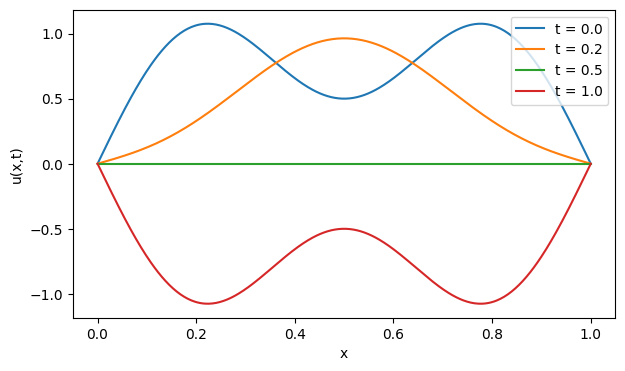
\includegraphics[width=0.6\textwidth]{sol-ondas-20nodos.png}
\caption{Solución de la ecuación de ondas en distintos instantes de tiempo,
obtenida mediante una truncación a $20$ modos normales.}
\label{fig:sol-ondas-20nodos}
\end{figure}
\begin{figure}[ht]
\centering
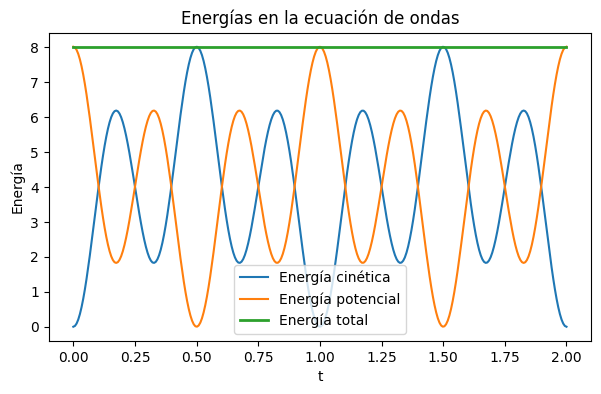
\includegraphics[width=0.6\textwidth]{energia-ondas.png}
\caption{Energía cinética, energía potencial y energía total de la solución de la
ecuación de ondas.}
\label{fig:energia-ondas}
\end{figure}


\section{La fórmula de d'Alembert}

Hasta ahora hemos estudiado la ecuación de ondas en dominios acotados, donde las
condiciones de contorno juegan un rol fundamental y la solución se construye
mediante series de Fourier. Veamos ahora el caso del dominio no acotado
$\R$, donde aparece una descripción particularmente simple de la solución.


Consideremos la ecuación de ondas en toda la recta
\begin{equation}\label{eq:ondasR}
u_{tt} - c^2 u_{xx} = 0,
\qquad x\in\R,\ t>0,
\end{equation}
con datos iniciales
\[
u(x,0)=g(x), \qquad u_t(x,0)=h(x).
\]

\subsection*{Cambio de variables característico}

Si introducimos las variables
\[
\xi = x - ct,
\qquad
\eta = x + ct,
\]
en estas coordenadas, un cálculo directo muestra que
\[
u_{tt} - c^2 u_{xx}
=
-4c^2\, u_{\xi\eta}.
\]
Por lo tanto, la ecuación de ondas \eqref{eq:ondasR} se reduce a
\[
u_{\xi\eta}=0.
\]
Esta ecuación tiene una solución inmediata de la forma
$$
u(\xi, \eta) = F(\xi) + G(\eta).
$$
donde $F$ y $G$ son funciones arbitrarias suficientemente regulares.

Si reescribimos esta solución en las variables originales, obtenemos
\[
u(x,t) = F(x-ct) + G(x+ct),
\]
Esta expresión muestra que toda solución es la superposición de dos ondas viajeras que se propagan sin deformarse, una hacia la derecha y otra hacia la izquierda, ambas con velocidad $c$.


\subsection*{Determinación de la solución a partir de los datos iniciales}

A partir de la forma general
\[
u(x,t)=F(x-ct)+G(x+ct),
\]
imponemos ahora las condiciones iniciales
\[
u(x,0)=g(x), \qquad u_t(x,0)=h(x).
\]

Evaluando en $t=0$ se obtiene
\[
F(x)+G(x)=g(x),
\]
mientras que derivando respecto del tiempo resulta
\[
u_t(x,t)=-cF'(x-ct)+cG'(x+ct),
\]
y por lo tanto
\[
-cF'(x)+cG'(x)=h(x).
\]

Derivando la primera igualdad obtenemos el siguiente sistema de ecuaciones para $F'(x)$ y $G'(x)$
\[
\begin{cases}
F'(x)+G'(x)=g'(x),\\[4pt]
-cF'(x)+cG'(x)=h(x),
\end{cases}
\]
del cual se deduce
\[
F'(x)=\frac12\Big(g'(x)-\frac{1}{c}h(x)\Big),
\qquad
G'(x)=\frac12\Big(g'(x)+\frac{1}{c}h(x)\Big).
\]

Integrando estas expresiones y absorbiendo las constantes de integración en la
definición de $F$ y $G$, se obtiene finalmente la \emph{fórmula de d'Alembert}:
\begin{equation}\label{eq:dalembert}
u(x,t)
=
\frac12\big(g(x-ct)+g(x+ct)\big)
+
\frac{1}{2c}
\int_{x-ct}^{x+ct} h(s)\,ds.
\end{equation}

\begin{obs}
La deducción de la fórmula de d’Alembert no sólo proporciona una representación explícita de la solución, sino que también implica la unicidad del problema de Cauchy, ya que cualquier solución suficientemente regular debe coincidir con dicha expresión.
\end{obs}

Una consecuencia inmediata de la fórmula de d'Alembert es la siguiente estimación de estabilidad
\begin{prop}[Estabilidad en norma supremo]
Sea $u$ la solución de la ecuación de ondas en $\R$ dada por la fórmula de
d'Alembert \eqref{eq:dalembert}, con datos iniciales
\[
u(x,0)=g(x), \qquad u_t(x,0)=h(x),
\]
donde $g,h\in L^\infty(\R)$. Entonces, para todo $T>0$ se verifica la estimación
\[
|u(x,t)| \le \|g\|_\infty + T\,\|h\|_\infty,
\qquad
\forall\,x\in\R,\ \forall\,t\in[0,T].
\]
\end{prop}

\begin{proof}
Por la fórmula de d'Alembert, la solución viene dada por
\[
u(x,t)
=
\frac12\bigl(g(x-ct)+g(x+ct)\bigr)
+
\frac{1}{2c}\int_{x-ct}^{x+ct} h(s)\,ds.
\]

Tomando valor absoluto y estimando término a término, obtenemos
\[
\left|\frac12\bigl(g(x-ct)+g(x+ct)\bigr)\right|
\le
\frac12\bigl(|g(x-ct)|+|g(x+ct)|\bigr)
\le
\|g\|_\infty,
\]
y
\[
\left|\frac{1}{2c}\int_{x-ct}^{x+ct} h(s)\,ds\right|
\le
\frac{1}{2c}\int_{x-ct}^{x+ct} |h(s)|\,ds
\le
\frac{1}{2c}(2ct)\,\|h\|_\infty
=
t\,\|h\|_\infty.
\]

Sumando ambas estimaciones se concluye que
\[
|u(x,t)| \le \|g\|_\infty + t\,\|h\|_\infty.
\]
Finalmente, como $0\le t\le T$, se deduce la cota uniforme
\[
|u(x,t)| \le \|g\|_\infty + T\,\|h\|_\infty,
\]
para todo $x\in\mathbb{R}$ y todo $t\in[0,T]$.
\end{proof}

\subsection*{Dominio de dependencia y rango de influencia}

Una de las consecuencias más importantes de la fórmula de d'Alembert es que
permite identificar de manera precisa qué parte de los datos iniciales influye
en el valor de la solución en un punto dado del espacio-tiempo.

En efecto, por la fórmula de d'Alembert \eqref{eq:dalembert}, la solución en un
punto $(x,t)$ viene dada por
\[
u(x,t)
=
\frac12\bigl(g(x-ct)+g(x+ct)\bigr)
+
\frac{1}{2c}
\int_{x-ct}^{x+ct} h(s)\,ds.
\]
De esta expresión se deduce inmediatamente que el valor de $u(x,t)$ depende
únicamente de los valores de los datos iniciales $g$ y $h$ en el intervalo
\[
[x-ct,\,x+ct].
\]

\medskip

\paragraph{Dominio de dependencia.}
Se dice que el \emph{dominio de dependencia} del punto $(x,t)$ es el conjunto de
puntos del eje inicial $\{t=0\}$ cuyos valores influyen en $u(x,t)$. En el caso
de la ecuación de ondas en $\R$, dicho dominio es el intervalo
\[
D(x,t)=\{(s,0)\in\R\times\{0\}:\ |s-x|\le ct\}.
\]
Geométricamente, este conjunto corresponde a la intersección del cono
característico con el eje $t=0$. Ver Figura \ref{fig:dominio-dependencia}.

\begin{figure}[ht]
\centering
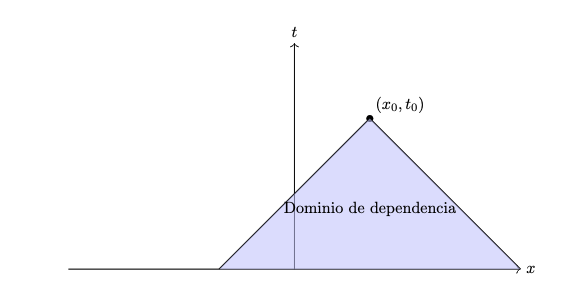
\includegraphics[width=0.6\textwidth]{dominio-dependencia.png}
\caption{Dominio de dependencia de un punto $(x_0,t_0)$ para la ecuación de ondas.
La solución en $(x_0,t_0)$ sólo depende de los valores iniciales dentro del intervalo
$[x_0-ct_0,x_0+ct_0]$.}
\label{fig:dominio-dependencia}
\end{figure}


\medskip

\paragraph{Rango de influencia.}
De manera dual, dado un punto $(x_0,0)$ del eje inicial, su \emph{rango de
influencia} es el conjunto de puntos $(x,t)$ tales que el valor de $u(x,t)$
depende del dato inicial en $(x_0,0)$. En este caso, dicho conjunto está dado por
\[
\{(x,t):\ |x-x_0|\le ct,\ t\ge 0\},
\]
que corresponde al cono característico con vértice en $(x_0,0)$. Ver Figura \ref{fig:rango-influencia}.

\begin{figure}[ht]
\centering
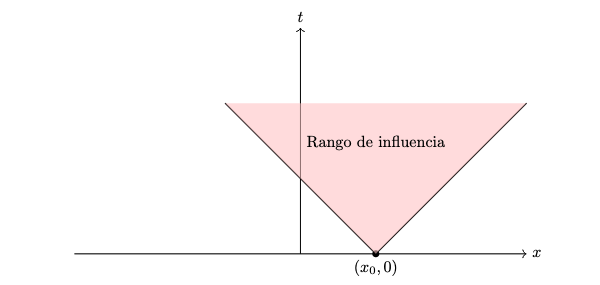
\includegraphics[width=0.6\textwidth]{rango-influencia.png}
\caption{Rango de influencia de un punto $(x_0,0)$ para la ecuación de ondas.
Una perturbación inicial localizada en $x_0$ sólo puede afectar a la solución
dentro del cono característico.}
\label{fig:rango-influencia}
\end{figure}

\medskip

Estas propiedades reflejan una característica fundamental de la ecuación de
ondas: la propagación de la información ocurre con velocidad finita $c$. En
particular, perturbaciones localizadas en los datos iniciales no se transmiten
instantáneamente a todo el espacio, en marcado contraste con lo que ocurre en
ecuaciones parabólicas como la ecuación del calor.

\begin{obs}
La existencia de dominios de dependencia y rangos de influencia finitos es una
manifestación de la naturaleza hiperbólica de la ecuación de ondas y está
íntimamente ligada a la unicidad y a la estabilidad del problema de Cauchy.
\end{obs}

\section{Dos descripciones de la misma solución}\label{sec:fourier-dalembert}

Tenemos dos fórmulas para la solución de la ecuación de ondas: la serie de Fourier en un intervalo y la fórmula de d'Alembert en la recta. No son dos teorías distintas: son la misma solución mirada de dos maneras.

Consideremos el problema en $(0,L)$ con condiciones de Dirichlet homogéneas y datos $g,h$, y extendamos $g$ y $h$ a toda la recta como funciones \emph{impares} y $2L$-periódicas (la extensión impar es la que se anula en $x=0$ y $x=L$). Sea $u$ la solución de d'Alembert \eqref{eq:dalembert} con esos datos extendidos. Entonces $u(\cdot,t)$ es impar y $2L$-periódica para todo $t$ (la fórmula preserva ambas simetrías; ejercicio), y por lo tanto $u(0,t)=u(L,t)=0$: la restricción de $u$ a $(0,L)$ es la solución del problema en el intervalo. Como por unicidad hay una sola, la serie de Fourier de la Sección anterior y esta $u$ coinciden.

La lectura física es transparente. Un pulso que viaja hacia la derecha sobre la cuerda llega al extremo fijo $x=L$, donde se encuentra con su ``imagen'' invertida que viene del intervalo $(L,2L)$ de la extensión impar: el resultado es que el pulso se \emph{refleja} en el extremo fijo con el signo cambiado. Una onda estacionaria (un modo normal) no es otra cosa que la superposición de dos ondas viajeras que se reflejan indefinidamente en los dos extremos. Recíprocamente, la fórmula $\sin(k\pi x/L)\cos(\omega_k t) = \frac12[\sin(k\pi(x-ct)/L) + \sin(k\pi(x+ct)/L)]$ muestra cada modo como suma de dos ondas viajeras.

\figpendiente{Reflexión de un pulso en un extremo fijo}{Instantes sucesivos de un pulso que viaja hacia el extremo fijo $x=L$ y se refleja invertido, junto con la extensión impar del dato inicial en $(L,2L)$ que ``explica'' la reflexión.}

Cada descripción es útil para algo distinto. La serie de Fourier hace evidentes las frecuencias, la energía por modo y el timbre; la fórmula de d'Alembert hace evidentes la velocidad finita de propagación, los dominios de dependencia y el hecho de que las singularidades del dato inicial \emph{viajan} sin suavizarse: si $g$ tiene un pico (una cuerda pulsada), $u(\cdot,t)$ tiene dos picos, en $x_0\pm ct$, para todo $t$. En la ecuación del calor, en cambio, todo pico desaparece instantáneamente. Esta es la diferencia cualitativa más profunda entre las ecuaciones parabólicas y las hiperbólicas, y conviene tenerla presente al elegir un modelo: si el fenómeno que se observa transporta perfiles sin deformarlos, el modelo es de ondas; si los borra, es de difusión.



\chapter{Ejercicios}

\section{Ejercicios teóricos}

\subsection*{Ecuación de difusión}


\begin{ejer} Sea $u$ una solución regular de $u_t - \Delta u = 0$ en
$\R^n\times (0,+\infty)$.
\begin{enumerate}
\item Mostrar que $u_{\lambda}(x,t)=u(\lambda x,\lambda^2 t)$ también
resuelve la ecuación del calor para cada $\lambda\in \R$.
\item Mostrar que $v(x,t)=x\cdot \nabla u(x,t) + 2tu_t(x,t)$ también
resuelve la ecuación del calor.
\end{enumerate}
\end{ejer}

\begin{ejer}
\begin{enumerate}
\item Si $\phi=\phi(x,t),\ x\in \R^3,\ t>0$, es una solución con
simetr\'\i a esférica de la ecuación del calor en $\R^3$ (i.e.
$\phi(x,t) = w(|x|,t)$ con $w:\R^2_+\to\R$), entonces $\phi$
satisface
\begin{equation}
\label{r}
\phi_{rr} + \frac{2}{r}\phi_r = \phi_t \quad t>0,\ r>0.
\end{equation}
\item Mostrar que la ecuación (\ref{r}) puede reducirse mediante el cambio
$\psi = r\phi$ a la ecuación del calor unidimensional.
\end{enumerate}
\end{ejer}

\begin{ejer}
Considerar el problema de la ecuación del calor con condiciones de tipo Neumann en el borde, es decir,
$$
\begin{cases}
u_t - u_{xx} = 0, & x\in (0,\pi),\ t>0,\\
u_x(0,t)=u_x(\pi, t)=0 & t>0,\\
u(x,0)=f(x) & x\in (0,\pi).
\end{cases}
$$
Encontrar la solución en forma de serie de Fourier.
\end{ejer}

%\begin{ejer} \emph{Solución fundamental}. Sea
%$$
%u(x,t) = \frac{1}{t^{\alpha}} v\left(\frac{x}{t^{\beta}}\right)\qquad (x\in \R^N,\ t>0),
%$$
%donde $\alpha$ y $\beta$ son constantes.
%\begin{enumerate}
%\item Verificar que $u$ satisface la ecuación del calor si y sólo si
%$v$ satisface
%$$\alpha t^{-(\alpha+1)}v(y) + \beta t^{-(\alpha+1)} y\cdot Dv(y) +
%t^{-(\alpha + 2\beta)} \Delta v(y) = 0,$$
%para $y = t^{-\beta} x$.
%\item Verificar que si $\beta = 1/2$, $v$ satisface
%$$\alpha v + \frac12 y\cdot Dv + \Delta v = 0.$$
%\item Verificar que si $v$ es radial, i.e. $v(y) = w(|y|)$ para
%$w:\R\to\R$, entonces $w$ satisface
%$$ \alpha w + \frac12 r w^\prime + w^{\prime\prime} + \frac{n-1}{r} w^\prime
%= 0,$$
%donde $r = |y|$, $ ^\prime = \frac{d}{dr}$.
%\item Tomar $\alpha = n/2$ y hallar la solución fundamental de la
%ecuación del calor.
%\end{enumerate}
%\end{ejer}

\begin{ejer}
Se quiere estudiar la evolución de la temperatura de una barra unidimensional de longitud $L$ que inicialmente está a temperatura constante $u_0>0$ y luego se mantiene uno de los extremos de la barra a temperatura constante $u_0$ mientras que el otro extremos se lo mantiene a temperatura constante $u_1>u_0$.

\begin{enumerate}
\item Observar que este problema se modela con la ecuación
$$
\begin{cases}
u_t - \kappa u_{xx} = 0, & x\in (0,L),\ t>0\\
u(x,0)=u_0, & x\in (0,L)\\
u(0,t)=u_0,\ u(L,t)=u_1
\end{cases}
$$

\item Antes de realizar cálculos especular con qué evolución se espera y cuál creen que será el estado final de la temperatura.

\item Considerar las variables adimensionales $y=x/L$ y $s=t/\tau$ donde $\tau = L^2/\kappa$ (recordar que las dimensiones del coeficiente de difusión $\kappa$ es $m^2/seg$).

Definir entonces la función rescalada 
$$
v(y,s)=\frac{u(Ly,\tau s)-u_0}{u_1-u_0}.
$$
Verificar que $v$ es solución del problema
$$\begin{cases}
v_s - v_{yy} = 0 & y\in (0,1),\ s>0\\
v(y,0)=0 & y\in (0,1)\\
v(0,t)=0, v(1,t)=1.
\end{cases}
$$

\item Calcular la solución estacionaria asociada al problema adimensional.

\item Si llamamos $v^*(y)$ a la solución estacionaria del ítem anterior, se define la función
$$
V(y,s) = v^*(y) - v(y,s)
$$ 
que mide el defecto de la solución del problema de evolución en alcanzar su estado estacionario. Verificar que $V$ es solución de la ecuación
$$\begin{cases}
V_s - V_{yy} = 0 & y\in (0,1),\ s>0\\
V(y,0)=y & y\in (0,1)\\
V(0,t)=0, V(1,t)=0.
\end{cases}
$$

\item Usar el método de separación de variables para calcular $V(y,s)$ para obtener la expresión
$$
V(y,s) = \sum_{j=1}^\infty (-1)^{j+1}\frac{2}{j\pi} e^{-j^2\pi^2 s} \sin(j\pi y).
$$

\item Volver a las variables originales y encontrar una expresión para $u(x,t)$. Observar que $u(x,t)$ converge, cuando $t\to\infty$ a la solución estacionaria asociada.

\item Observar que el término principal de la expresión obtenida para $u(x,t)$ es
$$
\frac{2}{\pi} e^{-\frac{\pi^2 \kappa t}{L^2}}\sin \frac{\pi}{L} x.
$$
Chequear que cuando $t\sim L^2/\kappa$ este término principal se redujo aproximadamente a un 0.005 \% de su amplitud original.

\item Concluir que el tiempo característico necesario para llegar al estado estacionario es del orden de $L^2/\kappa$.
\end{enumerate}
\end{ejer}

\begin{ejer}[Difusión con fuente de calor externa] La temperatura de una barra de longitud infinita con temperatura inicial $f$ y sujeta a una fuente de calor $g$ puede ser modelada por la ecuación:
$$\left\{\begin{array}{rcll}
u_t - k u_{xx} & = & g(x,t), & x\in \R,\ t>0,\\
u(x,0) & = & f(x), & x\in \R,\\
\end{array}\right.$$
donde $f$ y $g(\cdot,t)$ para cada $t$ fijo, son funciones de $\mathcal S$.

Usar la transformada de Fourier para resolver el problema.
\end{ejer}

\begin{ejer}[Difusión en barra semi-infinita] Encontrar la solución del problema
$$\left\{\begin{array}{rcll}
u_t & = & u_{xx}, & x>0,\ t>0,\\
u(x,0) & = & \varphi(x), & x\geq 0\\
u(0,t) & = & 0, & t> 0\\
\end{array}\right.$$
\end{ejer}

\begin{ejer} Sea $u(x,t)$ solución del problema
$$\left\{\begin{array}{rcll}
u_t & = & u_{xx}, & x\in \R,\ t>0,\\
u(x,0) & = & \varphi(x), & x\in \R\\
\end{array}\right.$$
dada por la convolución de $\varphi$ en la variable $x$ con la solución
fundamental. Probar que si $\varphi\in L^1(\R)$, entonces $u(\cdot,t)\in
L^1(\R)\ \forall t>0$ y
$$\int_{\R} u(x,t) dx = \int_{\R} \varphi(x) dx,\quad \forall t>0.$$
\end{ejer}


%\begin{ejer}
%Considerar la ecuación de Schr\"odinger
%$$
%\begin{cases}
%i u_t - u_{xx} = 0 & x\in\R, t>0,\\
%u(x,0)=f(x) & x\in\R.
%\end{cases}
%$$
%Comprobar que si $u$ es la solución obtenida por la transformada de Fourier, entonces se cumple que $u(x,t)\to f(x)$ cuando $t\to 0$ (en media cuadrática) y que $\int_{-\infty}^\infty |u(x,t)|^2\, dx$ es independiente de $t$.
%\end{ejer}


\subsection*{Transporte, reacción y difusión: el significado de cada término}

\begin{ejer}[Transporte]\label{ejer:transporte}
Consideramos la ecuación de difusión con transporte (o \emph{convección--difusión}) en la recta,
$$
u_t + v\,u_x = D\,u_{xx},\qquad x\in\R,\ t>0,\qquad u(x,0) = g(x),
$$
con $v\in\R$ y $D>0$.
\begin{enumerate}
\item Resolver primero el caso $D=0$: probar que $u(x,t) = g(x-vt)$. ¿Qué le hace el término $v u_x$ al perfil inicial? ¿Hacia dónde lo mueve si $v>0$?
\item Para $D>0$, hacer el cambio de variables $y = x-vt$, $w(y,t) = u(y+vt,t)$ y probar que $w$ resuelve la ecuación del calor. Deducir la solución explícita como convolución de $g$ con una gaussiana centrada en $vt$.
\item Graficar la solución para $g$ un pulso, con $v=1$ y $D=0.01$, $0.1$, $1$, en varios instantes. Describir en palabras qué hace cada término.
\item El cociente $\mathrm{Pe} = vL/D$ (el \emph{número de Péclet}) compara el transporte con la difusión en una escala espacial $L$. Verificar que es adimensional. Dar un ejemplo de fenómeno con $\mathrm{Pe}\gg 1$ y otro con $\mathrm{Pe}\ll 1$.
\item En dimensión $n$, con un campo de velocidades $\vv(\xx)$, hay dos formas de escribir el transporte: $\vv\cdot\nabla u$ y $\div(\vv u)$. Probar que coinciden si y sólo si $\div\vv = 0$, y que sólo la segunda conserva la masa total $\int u$ (cuando no hay flujo por el borde). ¿Cuál corresponde a un contaminante arrastrado por un fluido incompresible? ¿Y a una población que se mueve con velocidad dependiente de la posición?
\end{enumerate}
\end{ejer}

\begin{ejer}[Reacción]\label{ejer:reaccion}
Consideramos la ecuación de difusión con un término de reacción lineal,
$$
u_t = D\,u_{xx} + c\,u,\qquad c\in\R .
$$
\begin{enumerate}
\item Probar que si $u$ resuelve esta ecuación entonces $w = e^{-ct}u$ resuelve la ecuación del calor. Deducir que en la recta, $u(x,t) = e^{ct}(\Phi(\cdot,t)*g)(x)$. Interpretar: ¿qué hace el término $cu$ si $c>0$? ¿Y si $c<0$? Dar un ejemplo de cada caso (una población que se reproduce y se dispersa; una sustancia que se degrada mientras se difunde).
\item Mostrar que los tres efectos, difusión, transporte y reacción, se pueden desacoplar en el caso lineal: la solución de $u_t + vu_x = Du_{xx} + cu$ en $\R$ es $e^{ct}$ por la solución del calor evaluada en $x-vt$.
\item ¿Qué pasa con el cambio de variables del ítem 1 en un intervalo con condiciones de Dirichlet homogéneas? ¿Y con condiciones de Neumann? ¿Y de Robin?
\end{enumerate}
\end{ejer}

\begin{ejer}[Tamaño crítico de un hábitat]\label{ejer:habitat}
Una población que se reproduce con tasa $c>0$ y se dispersa con difusividad $D$ en un hábitat unidimensional $(0,L)$ rodeado de un ambiente hostil (donde muere instantáneamente) se modela con
$$
u_t = D\,u_{xx} + c\,u,\quad x\in(0,L),\qquad u(0,t)=u(L,t)=0,\qquad u(x,0)=g(x)\ge 0 .
$$
\begin{enumerate}
\item Resolver por separación de variables y escribir la solución en serie. Verificar que el modo $k$ evoluciona como $e^{(c - D k^2\pi^2/L^2)t}$.
\item Concluir que la población se extingue si $c<D\pi^2/L^2$ y crece exponencialmente si $c>D\pi^2/L^2$. Expresar el resultado como un \emph{tamaño crítico}: el hábitat sostiene a la población si y sólo si $L>L_c = \pi\sqrt{D/c}$.
\item Verificar que $L_c$ tiene unidades de longitud e interpretar: ¿por qué un hábitat más chico no alcanza, si la población se reproduce igual? ¿Qué papel juega $D$?
\item Comparar con el criterio de estabilidad del Capítulo \ref{ch:intro-heat}: el equilibrio $u\equiv 0$ es estable si y sólo si $c<D\lambda_1$, con $\lambda_1$ el primer autovalor de Dirichlet. Enunciar el resultado en un dominio $\Omega\subset\R^n$ cualquiera. ¿Cómo se relaciona con la bifurcación transcrítica de la Parte I?
\item El modelo lineal predice crecimiento exponencial sin límite. ¿Qué término habría que agregar para tener una capacidad de carga? (La ecuación resultante, $u_t = Du_{xx} + cu(1-u/K)$, se llama de Fisher--KPP.) ¿Cambia el tamaño crítico?
\end{enumerate}
\end{ejer}

\begin{ejer}[El operador general]
Sea $\LL u = D\Delta u - \vv\cdot\nabla u + cu$ en $\Omega\subset\R^n$. Para cada uno de los siguientes fenómenos, decir qué términos de $\LL$ intervienen, con qué signos, y qué condiciones de borde son razonables: (a) la temperatura de una barra con un extremo en un baño térmico y el otro al aire; (b) un contaminante vertido en un río; (c) un fármaco que se difunde en un tejido y es metabolizado; (d) una población de insectos en una isla; (e) el precio de una opción financiera (buscar la ecuación de Black--Scholes y reconocer los términos).
\end{ejer}

\subsection*{La temperatura del suelo}

\begin{ejer}[La solución periódica, paso a paso]\label{ejer:suelo-guiado}
Consideramos el problema \eqref{eq:suelo} con $T_s(t) = \bar T + A\cos(\omega t)$.
\begin{enumerate}
\item Verificar directamente que $u_{per}$ dado por \eqref{eq:suelo-periodica} resuelve la ecuación, la condición de borde y es acotada.
\item Probar que es la única solución acotada y periódica en $t$ (sugerencia: la diferencia $w$ de dos de ellas es acotada por $M$, periódica en $t$, se anula en $x=0$ y resuelve la ecuación del calor en el semieje; resolviendo desde el instante $t_0=-nT$ con la fórmula de la barra semi-infinita, $|w(x,t)|\le M\operatorname{erf}\bigl(x/\sqrt{4D(t-t_0)}\bigr)$, y esta cota tiende a cero cuando $n\to\infty$).
\item Calcular la profundidad a la que la amplitud del ciclo anual se reduce al $10\%$ y el retraso correspondiente, para $D = 5\times 10^{-7}$ m$^2$/s. ¿A qué profundidad la temperatura anual está en contrafase con la superficie?
\item Superponer los ciclos diario y anual y escribir $u_{per}$ para $T_s(t) = \bar T + A_1\cos(\omega_1 t) + A_2\cos(\omega_2 t + \phi)$.
\item ¿A qué profundidad hay que enterrar una cañería para que no se congele si la temperatura media anual es $12^\circ$C y la amplitud del ciclo anual en superficie es $15^\circ$C? ¿Cambia la respuesta si se considera además el ciclo diario?
\item Calcular el flujo de calor $-Du_x(0,t)$ en la superficie. ¿Está en fase con la temperatura? ¿Cuánto calor entra al suelo en verano y sale en invierno, por unidad de área?
\end{enumerate}
\end{ejer}

\subsection*{Ecuación de Laplace}

\begin{ejer}
Se considera el problema siguiente para la ecuación del potencial en el rectángulo $R=[0,a]\times[0,b]$:
$$
\begin{cases}
u_{xx} + u_{yy} = 0 & (x,y)\in R,\\
u(0,y)=u(a,y)=0, & y\in (0,b),\\
u(x,0)=f(x);\ u(x,b)=g(x) & x\in (0,a). 
\end{cases}
$$
Para cada $y$ fijo, se escribe $u(x,y)$ en serie de senos en el intervalo $(0,a)$ y se continúa como en los otros casos. Completar los cálculos.
\end{ejer}

\begin{ejer}
Buscamos funciones armónicas (i.e. que verifiquen $u_{xx} + u_{yy} = 0$) en el círculo unidad del plano conociendo su valor en la circunferencia. Escribiremos la solución en coordenadas polares, de modo que buscamos $u(r,\theta)$ para $0\le r<1$ y $0\le \theta\le 2\pi$. Verificar que el problema a resolver es
$$
\begin{cases}
u_{rr} + \frac{1}{r}u_r + \frac{1}{r^2}u_{\theta\theta} = 0 & 0\le r<1,\ 0\le \theta\le 2\pi,\\
u(1,\theta)=f(\theta) & 0\le \theta\le 2\pi.
\end{cases}
$$
Para cada $r$ fijo, desarrollamos $u(r,\theta)$ en serie de Fourier y tenemos
$$
u(r,\theta)= \frac{A_0(r)}{2} + \sum_{k=1}^\infty (A_k(r)\cos k\theta + B_k(r)\sin k\theta).
$$
Escribir las ecuaciones diferenciales ordinarias que deben satisfacer $A_k(r)$ y $B_k(r)$ y resolverlas; eliminar las soluciones que no sean continuas en el origen. Las constantes indeterminadas se obtienen a partir de $f$ y la solución obtenida debe ser
$$
\frac{a_0}{2} + \sum_{k=1}^\infty r^k (a_k\cos k\theta + b_k \sin k\theta),
$$
donde $a_k$ y $b_k$ son los coeficientes de Fourier de $f$.
\end{ejer}


\begin{ejer}[Efecto regularizante] 
Probar que si $u$ es armónica en $\Omega$, entonces las derivadas de cualquier orden de $u$ también son armónicas en $\Omega$.
\end{ejer}

\begin{ejer}[Problema de torsión] Si $\Omega\subset \R^2$ es un conjunto abierto y acotado y $v\in C^2(\Omega)\cap C^1(\overline\Omega)$ es solución del 
$$
\left\{
\begin{array}{rcll}
v_{xx} + v_{yy} & = & -2, & \text{ en } \Omega\\
v & = & 0, & \text{ en } \partial\Omega\\
\end{array}
\right.
$$
probar que $u=|\nabla v|^2$ alcanza su máximo en $\partial\Omega$.
\end{ejer}

%\item Sea $u\in C^2(B_1(0))\cap C(\overline{B_1(0)})$ una solución   de 
%$$
%\begin{cases}
%\Delta u = f & \text{en } B_1(0)\\
%u = g & \text{en } \partial B_1(0).
%\end{cases}
%$$
%Probar que existe una constante $C$, que depende sólo de la dimensión del espacio, tal que
%$$
%\max_{\overline{B_1(0)}}|u| \le C\left( \max_{\partial B_1(0)} |g| + \max_{\overline{B_1(0)}} |f| \right).
%$$
%?`Es cierta la conclusión del ejercicio si cambiamos $B_1(0)$ por $\Omega$ un dominio acotado cualquiera?
%


\begin{ejer}[Problema de Neumann]  Sea $\Omega$ un dominio con borde regular. Probar que si $u\in C^2(\Omega)\cap C^1(\bar{\Omega})$ es solución de
$$\begin{cases}
\Delta u = 0 & \text{en } \Omega,\\
\frac{\partial u}{\partial \nu}  = 0 & \text{en } \partial \Omega,
\end{cases}$$
entonces $u$ es constante.
\end{ejer}

\begin{ejer}[Problema de Neumann] Probar que si $\Omega$ es un abierto acotado de $\R^n$ y la ecuación
$$\begin{cases}
\Delta u = f & \text{en } \Omega, \\
\frac{\partial u}{\partial \nu} = g & \text{en } \partial \Omega,
\end{cases}$$
tiene una solución $u\in C^2(\Omega)\cap C^1(\bar{\Omega})$, entonces
$$
\int_{\Omega}f(x)dx=\int_{\partial \Omega}g(x)\, dS.
$$
\end{ejer}


 
 
%\medskip
%
%\item Sea $u$ una función armónica en un abierto y acotado $\Omega\subset\R^n$, y sea $x_0\in \Omega$. Probar que $u_{x_i}$ es armónica en $x_0$ para cada $1\leq i \leq n$ y que vale la estimación
%$$
%|\nabla u(x_0)| \leq n^\frac32 \frac{\sup_{x\in\Omega} |u|}{\inf_{y\in\partial\Omega} |x_0-y|}.
%$$

%\medskip
%
%\item Sea $\Omega\subset \R^n$ un abierto acotado y $u\in C^2(\Omega)\cap C(\overline\Omega)$ solución de 
%$$\begin{cases}
%\Delta u = u^3-u & \text{en } \Omega,\\
% u = 0 & \text{en } \partial \Omega,
%\end{cases}$$
%Mostrar que $-1\leq u(x)\leq 1$ para todo $x\in\Omega$.







\begin{ejer}[El esquema de cinco puntos es el juego]
Discretizamos el cuadrado $Q=[0,1]^2$ con paso $h=1/n$ y buscamos $U_{ij}\approx u(x_i,y_j)$ resolviendo el sistema lineal
$$
U_{ij} = \frac14\bigl(U_{i+1,j}+U_{i-1,j}+U_{i,j+1}+U_{i,j-1}\bigr)\ \text{ en los nodos interiores},\qquad U_{ij} = g(x_i,y_j) \ \text{ en el borde}.
$$
\begin{enumerate}
\item Verificar que este sistema es exactamente la ecuación del valor esperado del juego de la Sección \ref{sec:juego}, y también la discretización por diferencias centradas de $\Delta u = 0$ (Ejercicio \ref{ejer_dirichlet} en dos dimensiones).
\item Probar el \emph{principio del máximo discreto}: la solución $U$ alcanza su máximo y su mínimo en el borde. Deducir que el sistema tiene solución única.
\item Probar que la iteración $U^{(m+1)}_{ij} = \frac14\bigl(U^{(m)}_{i+1,j}+\cdots\bigr)$ (método de Jacobi) converge a la solución para cualquier $U^{(0)}$. Interpretarla como ``jugar un paso más''.
\end{enumerate}
\end{ejer}

\begin{ejer}[Laplace y los datos]
Los siguientes problemas de ciencia de datos son, en el fondo, la ecuación de Laplace o de Poisson.
\begin{enumerate}
\item \emph{Rellenar huecos (inpainting).} Una imagen $f$ en escala de grises tiene una región $\Omega$ dañada. Se propone rellenarla con la función $u$ armónica en $\Omega$ que coincide con $f$ en $\partial\Omega$. Explicar, usando la propiedad del valor medio y el principio del máximo, qué aspecto va a tener el relleno (¿puede crear un valor más claro que todo el borde?, ¿puede tener textura?). ¿Para qué tipo de regiones funciona bien y para cuáles no?
\item \emph{Propagación de etiquetas en un grafo.} Se tiene un grafo con $N$ nodos, de los cuales unos pocos están etiquetados con un valor $g_i\in\{0,1\}$. Se busca asignar a cada nodo no etiquetado el promedio de sus vecinos. Escribir el sistema lineal, compararlo con el juego de la Sección \ref{sec:juego} y probar que las etiquetas asignadas están en $[0,1]$. ¿Qué interpretación probabilística tiene $u_i$?
\item \emph{Suavizado variacional.} Dados datos ruidosos $d$ en $\Omega$, se busca $u$ que minimice $\frac12\int_\Omega|\nabla u|^2 + \frac{\mu}{2}\int_\Omega (u-d)^2$. Deducir, como en la Sección \ref{sec:minimas}, la ecuación de Euler--Lagrange $-\Delta u + \mu(u-d) = 0$ y la condición de borde natural ($\partial_\n u = 0$). ¿Qué hace el parámetro $\mu$? Resolver en un rectángulo con series de Fourier y mostrar que el método atenúa el modo $(k,\ell)$ por el factor $\mu/(\mu+\lambda_{k,\ell})$: es un filtro pasabajos.
\end{enumerate}
\end{ejer}

\subsection*{Ecuación de ondas}

\begin{ejer}
Utilizar la transformada de Fourier (en la variable $x$) para obtener la fórmula de d'Alembert para la ecuación de ondas en $\R$.
\end{ejer}

\begin{ejer}[Fórmula de D'Alambert] Verificar que el cambio de variables 
$$
\xi = x + ct,\qquad \eta = x - c t,
$$
transforma la ecuación de ondas $u_{tt} - c^2 u_{xx} = 0$ en
$$
\partial_\xi\partial_\eta u = 0.
$$
Usar este cambio de variables para hallar la fórmula de D'Alembert para la solución de la ecuación de ondas unidimensional.
\end{ejer} 


\begin{ejer}[Fuerzas externas]  El movimiento de una cuerda de longitud infinita que inicialmente está en reposo y se le aplica una fuerza externa dada por $h$ puede ser modelado de acuerdo a la siguiente ecuación:
$$
\begin{cases}
 u_{tt} - c^2  u_{xx} = h(x,t) & \text{en } \R \times(0,\infty),\\
u(x,0) =  u_t(x,0) = 0 & \text{en } \R.
\end{cases}
$$
Utilizar la transformada de Fourier para encontrar la solución.
\end{ejer}




\begin{ejer}[Cuerda semi-infinita] Consideramos una cuerda semi-infinita, esto es, situada sobre el semieje $x>0$ y amarrada al origen $x=0$. El movimiento de esta cuerda dada su posición inicial $g$ y su velocidad $h$ se puede modelar mediante la ecuación:
$$
\begin{cases}
 u_{tt} -  u_{xx} = 0 & x>0,\ t>0\\
u(0,t) = 0 & t>0\\
u(x,0) = g(x) & x>0\\
u_t(x,0) = h(x)& x>0.
\end{cases}
$$
Encontrar una fórmula explícita para la solución.
\end{ejer}

\begin{ejer}[La cuerda pulsada y la cuerda golpeada]\label{ejer:cuerda-guiado}
Consideramos la ecuación de ondas en $(0,L)$ con extremos fijos.
\begin{enumerate}
\item \emph{Cuerda pulsada.} Se suelta desde el reposo la forma inicial triangular $g(x) = a\,x/x_0$ para $x\le x_0$ y $g(x) = a\,(L-x)/(L-x_0)$ para $x\ge x_0$ (la cuerda tirada una distancia $a$ en el punto $x_0$). Calcular los coeficientes $A_k$ y verificar que $A_k = \frac{2aL^2}{\pi^2 x_0(L-x_0)}\,\frac{\sin(k\pi x_0/L)}{k^2}$. ¿Qué armónicos faltan si $x_0 = L/2$? ¿Y si $x_0=L/3$?
\item \emph{Cuerda golpeada.} La cuerda parte de la posición de equilibrio con velocidad inicial $h(x) = v_0$ en $(x_0-\epsilon,x_0+\epsilon)$ y cero en el resto. Calcular $B_k$ y su límite cuando $\epsilon\to 0$ con $2\epsilon v_0 = I$ fijo. Comparar el decaimiento de los coeficientes con el del ítem anterior y explicar por qué el piano tiene un sonido más ``rico'' en armónicos altos que la guitarra.
\item Verificar la fórmula \eqref{eq:energia-modos} y calcular la fracción de la energía en el modo fundamental en los dos casos anteriores, con $x_0 = L/5$.
\item Calcular la frecuencia fundamental de una cuerda de guitarra de $65$ cm y $3.5$ g/m sometida a una tensión de $70$ N. ¿Qué tensión hace falta para subirla un tono (un factor $2^{1/6}$)?
\end{enumerate}
\end{ejer}

\begin{ejer}[Amortiguamiento]
Consideramos la ecuación de ondas con fricción $u_{tt} + 2\gamma u_t = c^2u_{xx}$ en $(0,L)$ con extremos fijos, $\gamma>0$.
\begin{enumerate}
\item Probar que la energía $E$ de la Sección \ref{sec:energia-ondas} decrece: $E' = -2\gamma\int_0^L u_t^2\,dx$.
\item Separar variables y mostrar que el modo $k$ evoluciona como $e^{-\gamma t}\cos(\tilde\omega_k t - \phi_k)$ con $\tilde\omega_k = \sqrt{\omega_k^2-\gamma^2}$ (si $\gamma<\omega_k$). ¿Cambia la frecuencia? ¿Cambia el decaimiento de un modo a otro?
\item En una cuerda real los armónicos altos se apagan más rápido que los bajos. Proponer una modificación del término de fricción que reproduzca ese comportamiento (por ejemplo $-2\gamma u_t + \nu u_{xxt}$) y calcular la tasa de decaimiento de cada modo.
\item \emph{Inarmonicidad.} Una cuerda con rigidez a la flexión obedece $u_{tt} = c^2u_{xx} - \kappa u_{xxxx}$. Mostrar que los modos siguen siendo $\sin(k\pi x/L)$ pero las frecuencias pasan a ser $\omega_k = \frac{ck\pi}{L}\sqrt{1+\beta k^2}$ con $\beta = \kappa\pi^2/(c^2L^2)$. Los armónicos ya no son múltiplos enteros de la fundamental: ¿hacia dónde se corren? Esto se mide en el laboratorio.
\end{enumerate}
\end{ejer}

\begin{ejer}[Condición de Robin: un extremo atado a un resorte]
Consideramos la ecuación de ondas en $(0,L)$ con $u(0,t)=0$ y $u_x(L,t)+\kappa u(L,t) = 0$.
\begin{enumerate}
\item Separar variables y mostrar que las frecuencias propias son $\omega = c\mu$ donde $\mu$ resuelve $\tan(\mu L) = -\mu/\kappa$. Graficar ambos miembros y ubicar las raíces.
\item ¿Qué pasa con las frecuencias cuando $\kappa\to\infty$? ¿Y cuando $\kappa\to 0$? Interpretar físicamente ambos límites.
\item ¿Son los armónicos múltiplos enteros de la fundamental? ¿Suena ``afinada'' una cuerda así?
\end{enumerate}
\end{ejer}

\begin{ejer}[Equipartición de la energía]
Sea $u(x,t)$ la solución del problema de Cauchy para $u_{tt} - c^2u_{xx} = 0$ en $\R$ con datos $g,h$ suaves y de soporte compacto en $(a,b)$. Mostrar, usando la fórmula de d'Alembert, que existe $T$ tal que para $t\ge T$ la energía cinética $\int\frac12 u_t^2$ y la potencial $\int\frac{c^2}{2}u_x^2$ son iguales. Interpretar: para tiempos largos las dos ondas viajeras ya se separaron.
\end{ejer}

\begin{ejer}[Ondas viajeras y modos]
Verificar que, si $g$ y $h$ son las extensiones impares y $2L$-periódicas de datos en $(0,L)$, la fórmula de d'Alembert produce una función impar y $2L$-periódica en $x$ para todo $t$. Tomar $g(x) = \sin(\pi x/L)$, $h=0$, y comprobar que la fórmula de d'Alembert y la serie de Fourier dan la misma función. Repetir numéricamente con un pulso localizado y observar la reflexión en los extremos.
\end{ejer}

%\item \emph{Equiparación de la energía}. Sea $u(x,t)$ la solución de la ecuación de Cauchy  $u_{tt}-cu_{xx}=0$ con condición inicial $u(x,0)=g(x)$, $u_t(x,0)=h(x)$. Asumimos que $g$ y $h$ son funciones suaves con soporte compacto contenidos en el intervalo $(a,b)$. Mostrar que existe $T$ tal que, para $t\geq T$, 
%$$
%E_{cin}(t)=E_{pot}(t),
%$$
%donde las energías cinética y potencial se definen como
%$$
%E_{cin}(t)=\int_{-\infty}^\infty |u_t(x,t)|^2\,dx , \qquad E_{pot}(t)=\int_{-\infty}^\infty |u_x(x,t)|^2\,dx.
%$$
%
%\medskip

%\item \emph{Membrana circular. Tambor}. Una membrana elástica perfectamente flexible tiene la forma del círculo $B=\{(x,y)\colon x^2+y^2=1\}$. Si el borde de la membrana está fijo, y ésta tiene posición y velocidad inicial dadas por $g$ y $h$, respectivamente, entonces las vibraciones de la membrana están gobernadas por el siguiente sistema:
%$$
%\begin{cases}
% u_{tt} -  c^2(u_{rr} +\frac{1}{r}u_r + \frac{1}{r^2} u_{\theta\theta}) = 0 & 0<r<1, 0\leq \theta\leq 2\pi, t>0\\
%u(r,\theta,0) = g(r,\theta) & 0<r<1, 0\leq \theta\leq 2\pi\\
%u_t(r,\theta,0) = h(r,\theta) & 0<r<1, 0\leq \theta\leq 2\pi\\
%u(1,\theta,t)=0  & 0\leq \theta\leq 2\pi, t\geq0.
%\end{cases}
%$$
%\begin{enumerate}
%\item En el caso en que $h=0$ y $g=g(r)$, usar el método de separación de variables y probar que
%$$
%u(r,t)=\sum_{n=1}^\infty a_n J_0 (\lambda_n r)\cos \lambda_n t,
%$$
%donde $J_0$ es la función de Bessel de orden cero, $\lambda_1$, $\lambda_2, \ldots$ son los ceros de $J_0$ y el coeficiente $a_n$ está dado por
%$$
%a_n = \frac{2}{c_n^2}\int_0^1 sg(s)J_0(\lambda_n s)\,ds
%$$
%donde
%$$
%c_n = \sum_{k=1}^\infty \frac{(-1)^k}{k! (k+1)!}\left(\frac{\lambda_n}{2} \right)^{2k+1}.
%$$
%\end{enumerate}
%
%
%\end{enumerate} 
%
%
%\section*{Ecuación de transporte}
%
%\begin{enumerate}
%\item
%
%
%\newpage

\section{Ejercicios de laboratorio}

%1.---------
\begin{ejer}
Considerar los siguientes esquemas de diferenciación:
\begin{itemize}
  \item Diferencias forward: $u'(x) \sim \frac{u(x+h)-u(x)}{h}$.
  \item Diferencias backward: $u'(x) \sim \frac{u(x)-u(x-h)}{h}$.
  \item Diferencias centradas $u'(x) \sim \frac{u(x+h)-u(x-h)}{2h}$.
\end{itemize}
Implementar funciones que calculen matrices de diferenciación usando estos métodos:
\begin{itemize}
  \item Sobre un subconjunto adecuado de los nodos de una grilla de un cierto intervalo $[a,b]$,
  \item Sobre todos los nodos de la grilla, asumiendo condiciones de borde periódicas $u(a)=u(b)$. 
\end{itemize}
\end{ejer}

%----------------------------
%2.---------
\begin{ejer} Sea $u$ una función suficientemente suave. 
  \begin{enumerate}[label=(\alph*)]
    \item Calcular polinomios del grado adecuado que interpolen a $u$ en los nodos:
    \begin{itemize}
      \item $x-2h$, $x-h$ y $x$.
      \item $x-2h$, $x-h$, $x$, $x+h$ y $x+2h$.
    \end{itemize}
    \item Deducir fórmulas de diferencias finitas que aproximen $u'(x)$ utilizando esos nodos. 
    \item Implementar las matrices de diferenciación correspondientes asumiendo condiciones de contorno periódicas. 
  \end{enumerate}
\end{ejer}

%----------------------------
%3.---------
\begin{ejer} Evaluar numéricamente el orden de convergencia de los métodos de diferenciación de los ejercicios anteriores. Para ello, aplicar las matrices sobre una grilla con paso $h_i=2^{-i}$, $i=3,\dots,8$. Pueden utilizarse las siguientes funciones, en el intervalo $[0,1]$:
  \begin{itemize}
    \item $u(x) = \log(x+1)-\log(2)x$.
    \item $v(x) = e^{\cos(2\pi x)}$.
  \end{itemize}
Calcular el error en $\|\cdot\|_{\infty}$ y graficar el logaritmo del error en función del logaritmo de $h$ para estimar el orden de cada método. ¿Qué se observa cuando se aplican métodos que asumen condiciones de borde periódicas a la función $u$? ¿Por qué?
\end{ejer}

%----------------------------
%4.---------
\begin{ejer}[Condiciones de Dirichlet] \label{ejer_dirichlet}
Se desea resolver num\'ericamente la ecuaci\'on de Poisson en una dimensi\'on con
condiciones de borde de tipo Dirichlet
\begin{equation}
\label{laplaciano_dirichlet}
\left\lbrace
  \begin{array}{r l c}
      u_{xx}(x) = & f(x), & \mbox{para } x \in (0,1) \\
      u(0) = & \alpha & \\
      u(1) = & \beta. &
      \end{array}
    \right.
\end{equation}
Para ello se considera la malla uniforme $\{ x_j = hj, \; j=0,1,2,\dots m+1 \}$ con $h=1/(m+1)$.
Para los puntos de la malla $x_j \in (0,1)$ El esquema de diferencias centradas para
la derivada segunda:
\[
u''(x) \sim \frac{u(x+h)-2u(x)+u(x-h)}{h^2}.
\]
\begin{enumerate}[label=(\alph*)]
 \item Escribir un programa que resuelva el problema generando la matriz del  discreto con el comando \lstinline{np.diag}
 \item Repetir utilizando el comando \lstinline{scipy.sparse.spdiags}. 
 \item Comparar la performance de ambas resoluciones computando el tiempo de resolución (se puede usar el comando \lstinline{time.time()}) en función de $h$.
\end{enumerate}
\end{ejer}

\begin{ejer}[Capa l\'imite en el borde] \label{ejer_boundary_layer}
Considerar la ecuaci\'on
\begin{equation}
\label{boundary_layer}
 \varepsilon u_{xx} - u_{x} = f, \hspace{1cm} u(0)=\alpha \ \ \ u(1)=\beta.
\end{equation}
cuya soluci\'on exacta para el caso $f(x) = -1$ est\'a dada por
$$ u_{\varepsilon}(x) = \alpha + x + (\beta - \alpha -1) \left( \frac{e^{x/\varepsilon}-1 }{e^{1/\varepsilon}-1} \right)$$

\begin{enumerate}[label=(\alph*)]
\item Graficar la soluci\'on exacta para el caso $\alpha=1,\beta=3$ a medida que $\varepsilon \to 0$.
Interpretar el singnificado del t\'ermino \textit{capa l\'imite} que se suele aplicar al comportamiento
de $u_\varepsilon(x)$ para $x$ cerca del borde $\{ x=1 \}$ y $\varepsilon \to 0$.
¿De qu\'e tamaño es la \textit{capa l\'imite}?
\item Resuelva num\'ericamente la ecuación \eqref{boundary_layer} usando diferencias centradas para las
derivadas primera y segunda, y una malla de tamaño $h$. Grafique el error para distintos valores de $h$ y $\varepsilon$.
¿Qué ocurre si $h>>2\varepsilon$?
\end{enumerate}
\end{ejer}


%----------------------------
%5.---------
\begin{ejer}[Condiciones de Neumann] Se desea resolver num\'ericamente la ecuaci\'on de Poisson en una
dimensi\'on con condiciones de Neumann en $x=0$ y de Dirichlet en $x=1$,
\begin{equation}
\label{laplaciano_neumann}
\left\lbrace
  \begin{array}{r l r}
      u_{xx}(x) = & f(x), & \mbox{para } x \in (0,1) \\
      u_x(0) = & 0 & \\
      u(1) = & 0. &
      \end{array}
    \right.
\end{equation}
Obtener matrices para el problema discreto y resolver discretizando la condici\'on de Neumann $u_x(0)=0$ con las siguientes aproximaciones:
\begin{enumerate}[label=(\alph*)]
 \item $U_1 - U_0 = 0$ (diferencias forward)
 \item $U_1 - U_{-1} = 0$ (diferencias centradas y nodo ficticio)
 \item $\frac{3}{2}U_0 - 2U_1 + \frac{1}{2}U_2$ (diferencias forward de orden 2)
 \end{enumerate}
 \textbf{Sug.} Para el caso del nodo ficticio, añadir la ecuaci\'on $1/h^2\left(U_{-1} -2U_0 + U_{1}\right) = f(x_0)$.
 Comparar contra la soluci\'on exacta en el caso $f=\sin(2\pi x)$ y tomando $e_m = \| U - u \|_\infty$,
 estudiar num\'ericamente cu\'al es el orden de aproximaci\'on que se observa para la soluci\'on del problema en cada caso.
\end{ejer}

%----------------------------
%6.---------
\begin{ejer}\label{forward} Para aproximar la ecuaci\'on $U_t=\alpha U_{xx}$ se utiliza el esquema en
diferencias finitas que se obtiene al realizar una discretizaci\'on expl\'icita en la variable
temporal y diferencias centradas para la segunda derivada espacial:
\[ u_j^{n+1}=ru_{j-1}^n+(1-2r)u_j^n+ru_{j+1}^n \ \ \ \mbox{donde }r=\alpha\frac
{\Delta t}{(\Delta x)^2}=\alpha\frac{k}{h^2}.\]

\begin{enumerate}[label=(\alph*)]
\item Suponiendo que la solución  continua $U$ tiene derivadas continuas y acotadas de tanto orden como sea necesario, mostrar que para cualquier valor de $r>0$ fijo se tiene que: 
\[T_j^n:=\frac{U(x_j,t_{n+1}-U(x_j,t_n)}{k}-\alpha\frac{U(x_{j+1},t_n)-2U(x_j,t_n)+U(x_{j-1},t_n)}{h^2}\sim O(h^2)\]
Más aún: si se elige $r=\frac{1}{6}$ $T_j^n\sim O(h^4)$.
\item Mostrar que el error $e_j^{n}=U(x_j,t_n)-u_j^n$ satisface:
\[e_j^{n+1}=re_{j-1}^n+(1-2r)e_j^n+re_{j+1}^n +kT_j^n\]
Observar que el hecho de que $T_j^n\sim O(h^2)$ no garantiza la convergencia del método. 
\item Probar que  si $0<r\leq 1/2$ entonces el error global $E_n$ dado por
 $$ E_n=\max_{0\leq j \leq N} \{|e^n_j|\}, $$
 satisface la siguiente estimaci\'on en funci\'on del tiempo:
 $$ E_n\leq t M, $$
 donde $M$ es el valor m\'aximo de $|T|$. En particular, observe que
 si adem\'as $t\leq T_f$ y $U_{tt}$ y $U_{xxxx}$
 estan acotadas luego
 \begin{equation}\label{cota1}
 E_n\leq C T_f k
 \end{equation}
 para una constante $C$ independiente de $h$ y $k$.

\end{enumerate}
\end{ejer}

%-------------------------------
% Ejercicio 7
\begin{ejer} \label{programita}
El objetivo de este ejercicio es testear la necesidad de la condición $r<\frac{1}{2}$ obtenida en el ejercicio anterior. Escribir un programa para integrar con el m\'etodo expl\'{\i}cito del
ejercicio anterior la ecuaci\'on del calor $u_t=u_{xx}$ en el intervalo $[0,1]$ para un dato
inicial $u(x,0) = u_0(x)$ arbitrario y con condiciones de borde de tipo Dirichlet homogeneas.

\begin{enumerate}[label=(\alph*)]
 \item Resolver el caso $u_0(x) = x\chi_{[0,1/2]} + (1-x)\chi_{[1/2,1]}$.

 Para ello, considerar $h=0.05$,  $k=0.0012$, y $k=0.0013$. Avanzar por lo menos
50 pasos. ¿Qué sucede? Verificar el valor de $r$ en cada caso.

\item Ahora, tomando $k=0.0013$ resolver con dato inicial:
\begin{itemize}
\item $u(x,0)= x(1-x), $
\item $u(x,0)= \sin (\pi x). $
\end{itemize}

Observar que ambos casos resultan estables en los primeros 50
pasos. ¿Qu\'e ocurre con (i) para 100 pasos? \textquestiondown Y con (ii)? \textquestiondown
Por qu\'e resulta mucho m\'as estable este último caso?

\item Elegir uno de los casos anteriores y resolver anal\'iticamente.
Estudiar el error del m\'etodo contra la solucion exacta hasta el
tiempo $T_f=1$. Para ello, tomar $r=0.5$, diversos pasos de discretizaci\'on
$\Delta  t$ y $\Delta  x$, y graficar $\log(E_n)$ en cada paso de tiempo, donde
$E_n= \max_{ \{ 0\leq j \leq N \} } \{|e^n_j|\}$, $N=1/(\Delta x)$.

\textbf{Nota:} Observar que el error decrece a medida que el tiempo avanza lo que indica que la
cota \eqref{cota1} obtenida en el ejercicio anterior no es demasiado buena.
\end{enumerate}
\end{ejer}

%-------------------------------
% Ejercicio 7
\begin{ejer} Implementar el método implícito para la ecuación del Problema \ref{forward} (es decir: utilizando diferencias backward en el tiempo). Repetir el análisis del Problema \ref{programita}. ¿Qué se observa? 
\end{ejer}




\subsection*{Ecuación de ondas}

\begin{ejer}[Esquema explícito para la ecuación de ondas]\label{lab:leapfrog}
Para $u_{tt} = c^2u_{xx}$ en $(0,L)$ con extremos fijos se propone el esquema centrado en tiempo y espacio (\emph{leapfrog})
$$
u_j^{n+1} = 2u_j^n - u_j^{n-1} + r^2\bigl(u_{j+1}^n - 2u_j^n + u_{j-1}^n\bigr),\qquad r = \frac{c\,\Delta t}{\Delta x}.
$$
\begin{enumerate}
\item Deducirlo a partir de las diferencias centradas para $u_{tt}$ y $u_{xx}$. ¿Cómo se inicializa el primer paso a partir de $g$ y $h$?
\item Implementarlo para una cuerda pulsada y comparar con la solución en serie del Ejercicio \ref{ejer:cuerda-guiado} para $r = 0.5$, $r=1$ y $r=1.05$. ¿Qué se observa en cada caso? La condición $r\le 1$ (\emph{condición CFL}, de Courant, Friedrichs y Lewy) es necesaria para la estabilidad: explicarla en términos del dominio de dependencia (el esquema numérico debe ``ver'' al menos lo que ve la ecuación).
\item Calcular la energía discreta en cada paso y verificar que se conserva (aproximadamente) cuando $r<1$.
\item Simular la reflexión de un pulso en un extremo fijo y en un extremo libre ($u_x=0$). Comparar con la Sección \ref{sec:fourier-dalembert}.
\end{enumerate}
\end{ejer}

\subsection*{Laboratorio: los problemas conductores}

\begin{ejer}[La temperatura del suelo: ajuste de la difusividad]\label{lab:suelo}
Se proveen (con el notebook correspondiente) registros de temperatura del suelo a varias profundidades, tomados cada hora durante un año, junto con la temperatura del aire (o del suelo en superficie).
\begin{enumerate}
\item Graficar una semana de datos a todas las profundidades. Observar la atenuación y el retraso del ciclo diario.
\item Para cada profundidad $x$, calcular con la DFT la amplitud $A(x)$ y la fase $\phi(x)$ del ciclo diario y del ciclo anual (Parte II).
\item Según \eqref{eq:suelo-periodica}, $\ln A(x)$ y $\phi(x)$ son funciones lineales de $x$ con pendientes $-1/\delta$ y $1/\delta$. Ajustar ambas rectas por mínimos cuadrados y obtener dos estimaciones de $\delta$ (y por lo tanto de $D = \omega\delta^2/2$) para cada ciclo. ¿Coinciden las cuatro estimaciones? ¿Deberían?
\item Con el $D$ estimado, simular el problema \eqref{eq:suelo} con el esquema explícito del Ejercicio \ref{programita} usando la temperatura medida en superficie como condición de borde, y comparar con las mediciones a cada profundidad. Graficar los residuos. ¿Dónde y cuándo falla el modelo? (Pensar en la humedad del suelo, la lluvia, la nieve, la radiación.)
\item Repetir el ajuste usando sólo un mes de datos. ¿Cuánto cambia $D$? Discutir qué precisión es razonable esperar.
\end{enumerate}
\end{ejer}

\begin{ejer}[El espectro de una cuerda real]\label{lab:cuerda}
\begin{enumerate}
\item Grabar con un teléfono (o descargar) el sonido de una cuerda de guitarra pulsada, unos $3$ segundos, y cargar el archivo de audio en Python (\lstinline{scipy.io.wavfile}).
\item Calcular el espectro de potencia del primer medio segundo. Identificar la frecuencia fundamental $f_1$ y los picos siguientes. ¿Están en $kf_1$? Medir el corrimiento relativo $(f_k - kf_1)/(kf_1)$ y compararlo con la predicción de inarmonicidad del ejercicio de amortiguamiento: ¿crece como $k^2$?
\item Calcular el espectrograma (Parte II) y medir la tasa de decaimiento de cada armónico. ¿Decaen todos igual? Proponer un término de fricción en el modelo que reproduzca lo observado.
\item Repetir pulsando la cuerda en el medio y cerca del puente. Comparar el reparto de energía entre armónicos con la predicción del Ejercicio \ref{ejer:cuerda-guiado}.
\item Simular la cuerda con el esquema del Ejercicio \ref{lab:leapfrog} (agregando el término de fricción propuesto), ``escuchar'' la simulación (escribir el archivo de audio) y comparar su espectro con el real. Escribir un párrafo con la conclusión: qué predice bien el modelo de la cuerda ideal, qué le falta y qué le agregaría.
\end{enumerate}
\end{ejer}

\begin{ejer}[Laplace en 2D: cinco puntos contra Monte Carlo]
Consideramos el problema de Dirichlet $\Delta u = 0$ en el cuadrado unitario con un dato de borde $g$ a elección (por ejemplo $g=1$ en el lado superior y $0$ en los otros tres).
\begin{enumerate}
\item Resolver el sistema lineal del esquema de cinco puntos con $n = 20, 40, 80$ (usar matrices ralas, \lstinline{scipy.sparse}). Graficar la solución como mapa de color.
\item Resolver el mismo problema ``jugando'': desde cada nodo interior, simular $M$ paseos al azar hasta llegar al borde y promediar el pago $g$. Comparar con el ítem anterior para $M=10, 100, 1000$. ¿Cómo decrece el error con $M$? ¿Cuál método es más caro?
\item Agregar una fuente: $-\Delta u = f$. ¿Cómo se modifica el juego? Verificar numéricamente.
\item \emph{Inpainting.} Tomar una imagen en escala de grises, borrar una región y rellenarla resolviendo la ecuación de Laplace con el borde de la región como dato. Mostrar el resultado para una región chica sobre un fondo liso y para una región grande sobre una textura. Explicar lo que se observa con el principio del máximo.
\end{enumerate}
\end{ejer}


\bibliography{biblio}
\bibliographystyle{amsplain}
\end{document}
